\documentclass[11pt,a4paper,UTF8]{ctexart}
% \usepackage{ctex}
\setCJKmainfont{SimSun}[AutoFakeBold=2]
\setCJKsansfont{SimHei}[AutoFakeBold=2]
\setCJKfamilyfont{zhsong}{SimSun}[AutoFakeBold=2]
\setCJKfamilyfont{zhhei}{SimHei}[AutoFakeBold=2]
\usepackage{graphicx}
\usepackage{amsmath}
\usepackage{amssymb}
\usepackage{booktabs}
\usepackage{tabularx}
\usepackage{float}
\usepackage{hyperref}
\setcounter{secnumdepth}{3}
\setcounter{tocdepth}{2}
\ctexset{
  section = {
    name = {,},
    number = \arabic{section},
    format = \Large\bfseries\heiti,
    aftername = \hspace{0.5em},
  },
  subsection = {
    name = {,},
    number = \thesection.\arabic{subsection},
    format = \large\bfseries\heiti,
    aftername = \hspace{0.5em},
  },
  subsubsection = {
    name = {,},
    number = \thesubsection.\arabic{subsubsection},
    format = \normalsize\bfseries\heiti,
    aftername = \hspace{0.5em},
  }
}
\renewcommand{\thesection}{\arabic{section}}
\renewcommand{\thesubsection}{\thesection.\arabic{subsection}}
\renewcommand{\thesubsubsection}{\thesubsection.\arabic{subsubsection}}
\numberwithin{figure}{section}
\numberwithin{table}{section}
\renewcommand{\thefigure}{\arabic{section}-\arabic{figure}}
\renewcommand{\thetable}{\arabic{section}-\arabic{table}}
\usepackage{listings}
\usepackage{geometry}
\usepackage{color}
\usepackage{xcolor}
\usepackage{enumitem}
\usepackage{titlesec}
\usepackage{indentfirst}
\usepackage{pifont}
\newcolumntype{C}[1]{>{\centering\arraybackslash}p{#1}}
\newcolumntype{Y}{>{\centering\arraybackslash}X}
\newcommand{\goalstar}{\ding{72}}

\geometry{left=2.5cm,right=2.5cm,top=2.5cm,bottom=2.5cm,headheight=15pt}
\setlength{\parindent}{2em}
\setlength{\parskip}{0.25em}
\setlist{leftmargin=2.2em,topsep=0.45em,itemsep=0.2em,parsep=0pt}
\setlist[itemize,1]{label={\small$\bullet$}}
\setlist[itemize,2]{label={\small--}}
\setlist[enumerate,1]{label={\bfseries\arabic*.}}
\setlist[enumerate,2]{label={(\arabic*)}}
\setlength{\abovecaptionskip}{0.5em}
\setlength{\belowcaptionskip}{0.5em}
\renewcommand{\arraystretch}{1.18}
\usepackage{fancyhdr}
\pagestyle{fancy}
\fancyhf{}
\chead{\nouppercase{\small\heiti\leftmark}}
\cfoot{\thepage}
\renewcommand{\headrulewidth}{0.4pt}

\definecolor{codegreen}{rgb}{0,0.6,0}
\definecolor{codegray}{rgb}{0.5,0.5,0.5}
\definecolor{codepurple}{rgb}{0.58,0,0.82}
\definecolor{backcolour}{rgb}{0.95,0.95,0.92}

% 统一标题左对齐与正文内部层级。
\titleformat{\section}[block]
  {\Large\bfseries\heiti\centering}
  {\thesection}{0.5em}{}
\titleformat{\subsection}[block]
  {\large\bfseries\heiti}
  {\thesubsection}{0.5em}{}
\titleformat{\subsubsection}[block]
  {\normalsize\bfseries\heiti}
  {\thesubsubsection}{0.5em}{}
\titleformat{\paragraph}[block]
  {\normalfont\bfseries\heiti}
  {}{0pt}{}
\titlespacing*{\section}{0pt}{2.0em}{0.8em}
\titlespacing*{\subsection}{0pt}{1.5em}{0.6em}
\titlespacing*{\subsubsection}{0pt}{1.2em}{0.5em}
\titlespacing*{\paragraph}{0pt}{1.1em}{0.4em}

\newcommand{\answerlabel}{%
  \par\smallskip\noindent{\heiti\bfseries 回答：}\quad}
\newcommand{\analysislabel}{%
  \par\smallskip\noindent{\heiti\bfseries 分析：}\quad}
\newcommand{\conclusionlabel}{%
  \par\smallskip\noindent{\heiti\bfseries 结论：}\quad}
\newcommand{\question}[1]{\par\smallskip\noindent\textbf{#1}\par}

\lstdefinestyle{mystyle}{
    backgroundcolor=\color{backcolour},
    commentstyle=\color{codegreen},
    keywordstyle=\color{blue},
    numberstyle=\tiny\color{codegray},
    stringstyle=\color{codepurple},
    basicstyle=\small\ttfamily,
    breakatwhitespace=false,         
    breaklines=true,                 
    captionpos=b,                    
    keepspaces=true,                 
    numbers=left,                    
    numbersep=5pt,                  
    showspaces=false,                
    showstringspaces=false,
    showtabs=false,                  
    tabsize=4
}
\lstset{style=mystyle}

\hypersetup{hidelinks}

\begin{document}

% ==================== Cover Page ====================
\begin{titlepage}
    \centering
    \vspace*{-0.8cm}
    
\includegraphics[width=0.4\textwidth]{HUSTBlack.eps} \\[1.5cm]
    {\fontsize{50pt}{60pt}\selectfont\songti\bfseries 课\hspace{0.4em}程\hspace{0.4em}实\hspace{0.4em}验\hspace{0.4em}报\hspace{0.4em}告} \\[4.9cm]
    
    \begin{tabular}{r@{\quad}l}
        {\fontsize{18pt}{22pt}\selectfont\heiti\bfseries \makebox[4em][s]{课程名称}：} & \underline{\makebox[5.7cm][c]{\fontsize{18pt}{22pt}\selectfont\songti\bfseries 强化学习}} \\[0.6cm]
        {\fontsize{18pt}{22pt}\selectfont\heiti\bfseries \makebox[4em][s]{实验名称}：} & \underline{\makebox[5.7cm][c]{\fontsize{18pt}{22pt}\selectfont\songti\bfseries 强化学习基础实验}} \\[3.2cm]
        {\fontsize{14pt}{18pt}\selectfont\songti\bfseries \makebox[4em][s]{院\hfill 系}：} & \underline{\makebox[4.7cm][c]{\fontsize{14pt}{18pt}\selectfont\songti\bfseries 计算机科学与技术}} \\[0.4cm]
        {\fontsize{14pt}{18pt}\selectfont\songti\bfseries \makebox[4em][s]{专业班级}：} & \underline{\makebox[4.7cm][c]{\fontsize{14pt}{18pt}\selectfont\songti\bfseries PROGRAM-CLASS}} \\[0.4cm]
        {\fontsize{14pt}{18pt}\selectfont\songti\bfseries \makebox[4em][s]{学\hfill 号}：} & \underline{\makebox[4.7cm][c]{\fontsize{14pt}{18pt}\selectfont\songti\bfseries U2023xxxxx}} \\[0.4cm]
        {\fontsize{14pt}{18pt}\selectfont\songti\bfseries \makebox[4em][s]{姓\hfill 名}：} & \underline{\makebox[4.7cm][c]{\fontsize{14pt}{18pt}\selectfont\songti\bfseries STUDENT-NAME}} \\[0.4cm]
        {\fontsize{14pt}{18pt}\selectfont\songti\bfseries \makebox[4em][s]{指导教师}：} & \underline{\makebox[4.7cm][c]{\fontsize{14pt}{18pt}\selectfont\songti\bfseries 马志远}} \\[2.2cm]
    \end{tabular}
    
    \vspace*{1cm}
    {\Large\songti \underline{\makebox[1.7cm][c]{\the\year}}~年~\underline{\makebox[0.7cm][c]{\the\month}}~月~\underline{\makebox[1.0cm][c]{\the\day}}~日}
\end{titlepage}

\newpage
\pagestyle{plain}
\tableofcontents
\newpage
\pagestyle{fancy}

\newpage
\section{值迭代和策略迭代}
\subsection{实验目的与要求}

\begin{enumerate}
\item 理解基于模型的强化学习核心思想，掌握贝尔曼方程与贝尔曼最优方程的数学原理，明确值函数与动作值函数的关系。
\item 掌握值迭代算法的原理与实现流程，理解其作为贝尔曼最优方程直接求解方法的本质。
\item 掌握策略迭代算法的原理与实现流程，理解策略评价与策略改进的交替迭代机制，掌握其收敛性证明的核心思路。
\item 掌握截断策略迭代算法的原理与实现流程，理解值迭代与策略迭代作为其特殊情况的关系，能够分析不同截断次数对算法性能的影响。
\item 能够在网格世界环境中实现上述三种算法，对比它们的收敛速度、计算效率与最终性能，加深对广义策略迭代思想的理解。
\end{enumerate}
\subsection{实验内容与设计}

\subsubsection{实验环境}

本实验在 $5\times5$ GridWorld 中进行，动作空间为上、下、左、右，折扣因子统一取 $\gamma=0.9$。任务 1 使用边界与禁止区域奖励 $-1$；任务 2 与任务 3 将禁止区域奖励设为 $-10$，用于观察策略对高代价区域的规避行为。

\begin{table}[H]
\centering
\begin{tabular}{cccc}
\toprule
设计项 & 值迭代 & 策略迭代 & 截断策略迭代 \\
\midrule
核心更新 & 贝尔曼最优更新 & 策略评价与改进 & 有限次策略评价与改进 \\
主要变量 & 初始值函数 & 策略评价阈值 & 截断次数 $j$ \\
评价指标 & 迭代次数、最大误差 & 外循环与评价步数 & 时间、迭代次数、误差 \\
\bottomrule
\end{tabular}
\end{table}

\subsubsection{任务 1：值迭代实验设计}

先在 $2\times2$ 网格中手工核对前三次 q-table 与值函数，验证更新实现；再在 $5\times5$ 环境中记录最大值函数变化量、最终值函数和策略。额外比较全零、随机和乐观初始值，分析初始化对收敛速度的影响。

\subsubsection{任务 2：策略迭代实验设计}

策略评价阶段迭代求解当前策略的状态值，策略改进阶段选择贪心动作。实验记录每次外循环的评价步数、值函数变化和策略演变，并按状态到目标的距离分析不同区域达到稳定策略的先后顺序。

\subsubsection{任务 3：截断策略迭代实验设计}

设置 $j_{\text{truncate}}\in\{1,3,5,10,\infty\}$，使用上一轮值函数作为下一轮评价初值。在相同精度要求下比较总迭代次数、运行时间和收敛曲线，以判断有限评价次数如何平衡单轮成本与外循环数量。




\subsection{实验过程、结果与分析}

\subsubsection{任务 1：值迭代算法}

值迭代（Value Iteration）直接迭代贝尔曼最优方程：

$$V_{k+1}(s) = \max_a \sum_{s'} p(s'|s,a)\bigl[r(s,a,s') + \gamma V_k(s')\bigr]$$

等价地，先计算所有动作的 Q 值，再取最大：

$$q_k(s,a) = \sum_{s'} p(s'|s,a)\bigl[r(s,a,s') + \gamma V_k(s')\bigr], \quad V_{k+1}(s) = \max_a\, q_k(s,a)$$

当 $\max_s |V_{k+1}(s)-V_k(s)|<\theta$ 时停止，本实验取 $\theta=10^{-6}$。收敛后按下式提取贪心策略：
\[
\pi(s)=\arg\max_a q(s,a)
\]

\paragraph{2×2 小网格手动验证}

为验证实现正确性，先在 2×2 网格（目标 (1,1)，无禁止区域）上手工核对前 3 次迭代：

\textbf{初始状态}：$V_0(s) = 0$ for all $s$

\textbf{迭代 1}（Q-Table）：

\begin{table}[H]
\centering
\begin{tabular}{ccccccc}
\toprule
状态 & ↑ & ↓ & ← & → & V(s) & $\pi(s)$ \\
\midrule
(0,0) & −1.000 & 0.000 & −1.000 & 0.000 & 0.000 & ↓ \\
(0,1) & −1.000 & \textbf{1.000} & 0.000 & −1.000 & 1.000 & ↓ \\
(1,0) & 0.000 & −1.000 & −1.000 & \textbf{1.000} & 1.000 & → \\
(1,1) \goalstar & 0 & 0 & 0 & 0 & 0 & — \\
\bottomrule
\end{tabular}
\end{table}

\textbf{迭代解释：}(0,1) 向下可到达目标得 +1；(1,0) 向右可到达目标得 +1；其余状态尚未传播到目标信息。

\textbf{迭代 2}（Q-Table）：

\begin{table}[H]
\centering
\begin{tabular}{ccccccc}
\toprule
状态 & ↑ & ↓ & ← & → & V(s) & $\pi(s)$ \\
\midrule
(0,0) & −1.000 & 0.900 & −1.000 & 0.900 & 0.900 & ↓ \\
(0,1) & −0.100 & \textbf{1.000} & 0.000 & −0.100 & 1.000 & ↓ \\
(1,0) & 0.000 & −0.100 & −0.100 & \textbf{1.000} & 1.000 & → \\
(1,1) \goalstar & 0 & 0 & 0 & 0 & 0 & — \\
\bottomrule
\end{tabular}
\end{table}

\textbf{迭代解释：}(0,0) 可以向下到 (1,0)（$V=1$），得 $0 + 0.9 \times 1 = 0.9$；向右到 (0,1)（$V=1$），同样 0.9。

\textbf{迭代 3}（Q-Table）：

\begin{table}[H]
\centering
\begin{tabular}{ccccccc}
\toprule
状态 & ↑ & ↓ & ← & → & V(s) & $\pi(s)$ \\
\midrule
(0,0) & −0.190 & 0.900 & −0.190 & 0.900 & 0.900 & ↓ \\
(0,1) & −0.100 & \textbf{1.000} & 0.810 & −0.100 & 1.000 & ↓ \\
(1,0) & 0.810 & −0.100 & −0.100 & \textbf{1.000} & 1.000 & → \\
(1,1) \goalstar & 0 & 0 & 0 & 0 & 0 & — \\
\bottomrule
\end{tabular}
\end{table}

第 3 次迭代后值函数不再变化（$\max|\Delta V|=0$），因此该 $2\times2$ 网格在第 3 次迭代达到收敛判据。

\paragraph{5×5 网格实验结果}

\textbf{收敛情况}：值迭代在 \textbf{9 次迭代}后收敛（max|ΔV| 降至 0）。

各次迭代 max|ΔV|：

\begin{table}[H]
\centering
\begin{tabular}{cccccccccc}
\toprule
迭代次数 & 1 & 2 & 3 & 4 & 5 & 6 & 7 & 8 & 9 \\
\midrule
max|ΔV| & 1.000 & 0.900 & 0.810 & 0.729 & 0.656 & 0.591 & 0.531 & 0.478 & 0.000 \\
\bottomrule
\end{tabular}
\end{table}

\textbf{最终值函数矩阵}（保留 4 位小数）：

\begin{lstlisting}[language=Python]
[[0.4783, 0.5314, 0.5905, 0.6561, 0.7290],
 [0.5314, 0.5905, 0.6561, 0.7290, 0.8100],
 [0.5905, 0.6561, 0.7290, 0.8100, 0.9000],
 [0.6561, 0.7290, 0.8100, 0.9000, 1.0000],
 [0.7290, 0.8100, 0.9000, 1.0000, 0.0000]]  ← 目标状态 V=0（终止）
\end{lstlisting}

\textbf{最终最优策略}：

\begin{lstlisting}[language=Python,escapeinside={(*@}{@*)}]
 ↓  →  ↓  ↓  ↓
 ↓  ↓  ↓  →  ↓
 ↓  ↓  ↓  ↓  ↓
 ↓  ↓  ↓  ↓  ↓
 →  →  →  →  (*@\goalstar@*)
\end{lstlisting}

\textbf{值函数热力图}：

\begin{figure}[H]
\centering
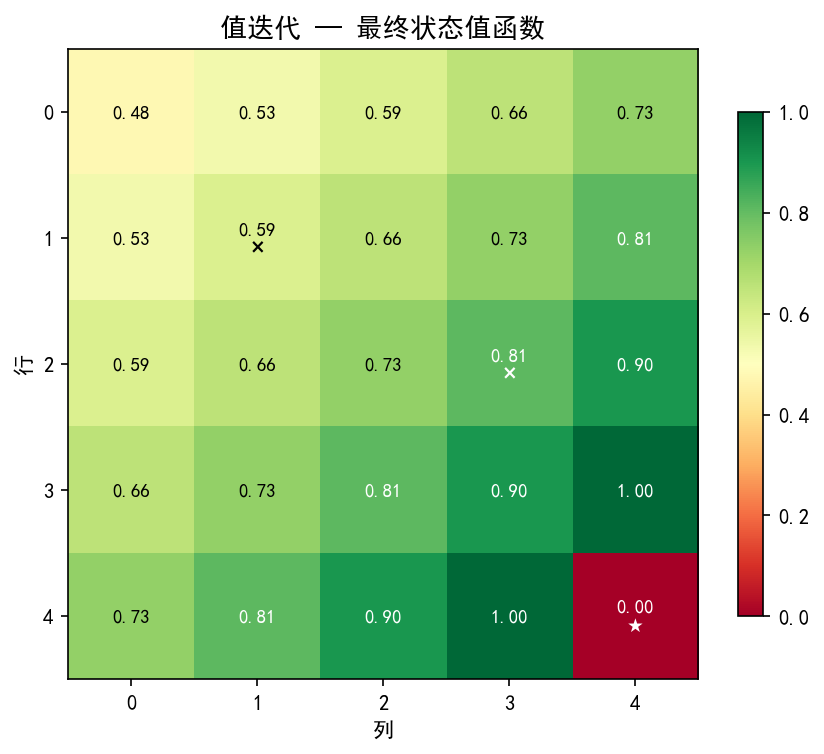
\includegraphics[width=0.5\textwidth]{exp1/results/task1_value_heatmap.png}
\caption{值函数热力图}
\end{figure}

\textbf{最优策略箭头图}：

\begin{figure}[H]
\centering
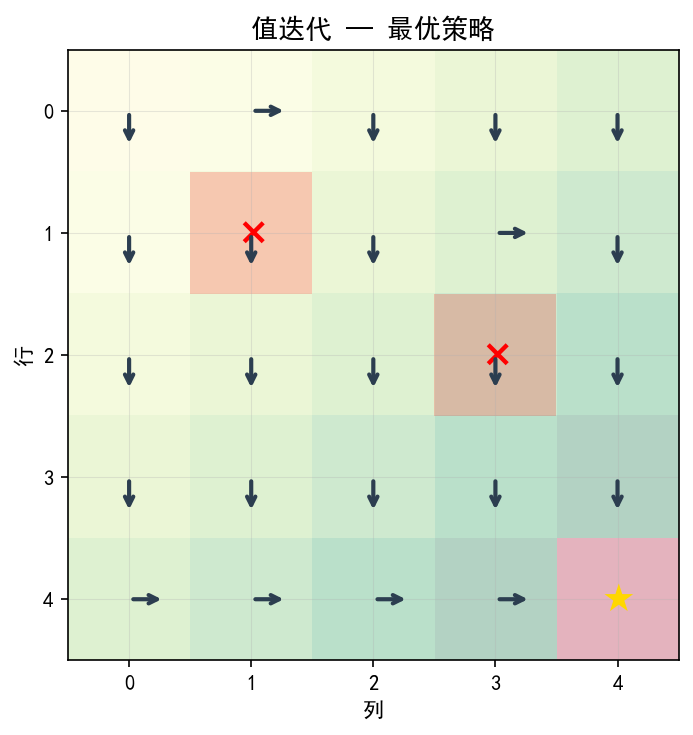
\includegraphics[width=0.5\textwidth]{exp1/results/task1_policy.png}
\caption{最优策略}
\end{figure}

\textbf{收敛曲线}：

\begin{figure}[H]
\centering
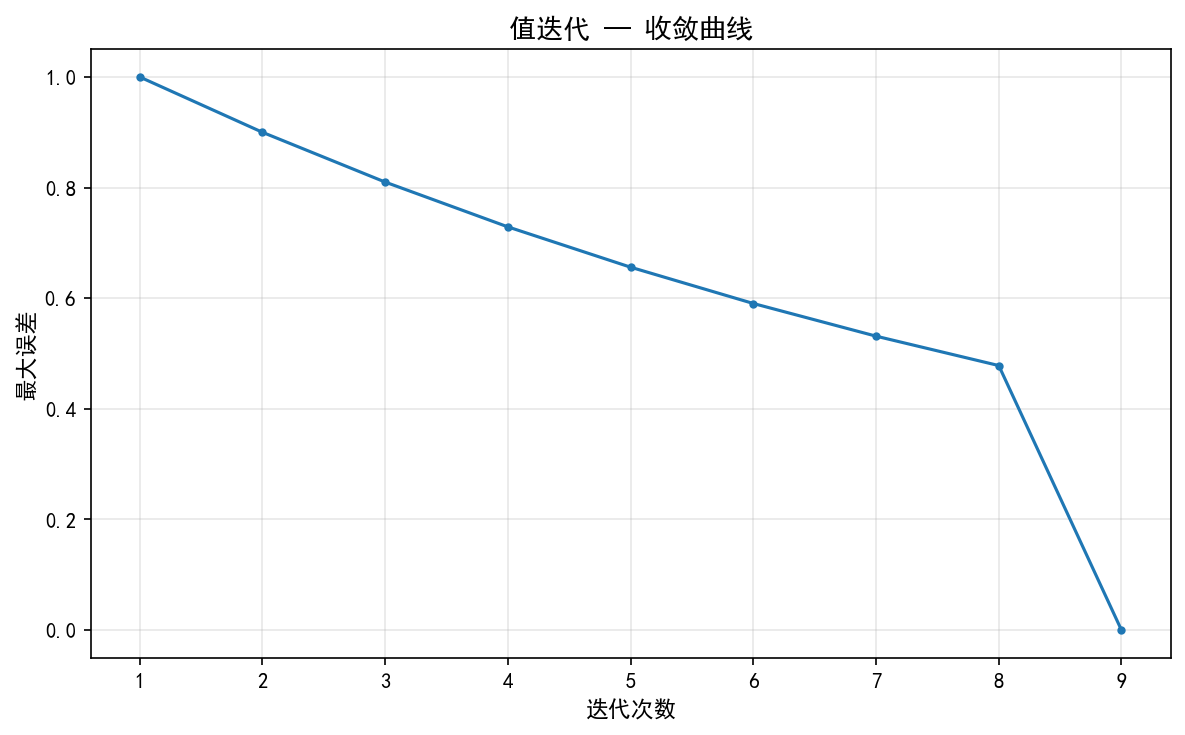
\includegraphics[width=0.7\textwidth]{exp1/results/task1_convergence.png}
\caption{收敛曲线}
\end{figure}

\paragraph{不同初始值函数对比}

\begin{table}[H]
\centering
\begin{tabular}{cc}
\toprule
初始值设置 & 收敛迭代次数 \\
\midrule
V=0（全零） & 9 \\
V=随机 & 12 \\
V=乐观（+5） & 26 \\
\bottomrule
\end{tabular}
\end{table}

\begin{figure}[H]
\centering
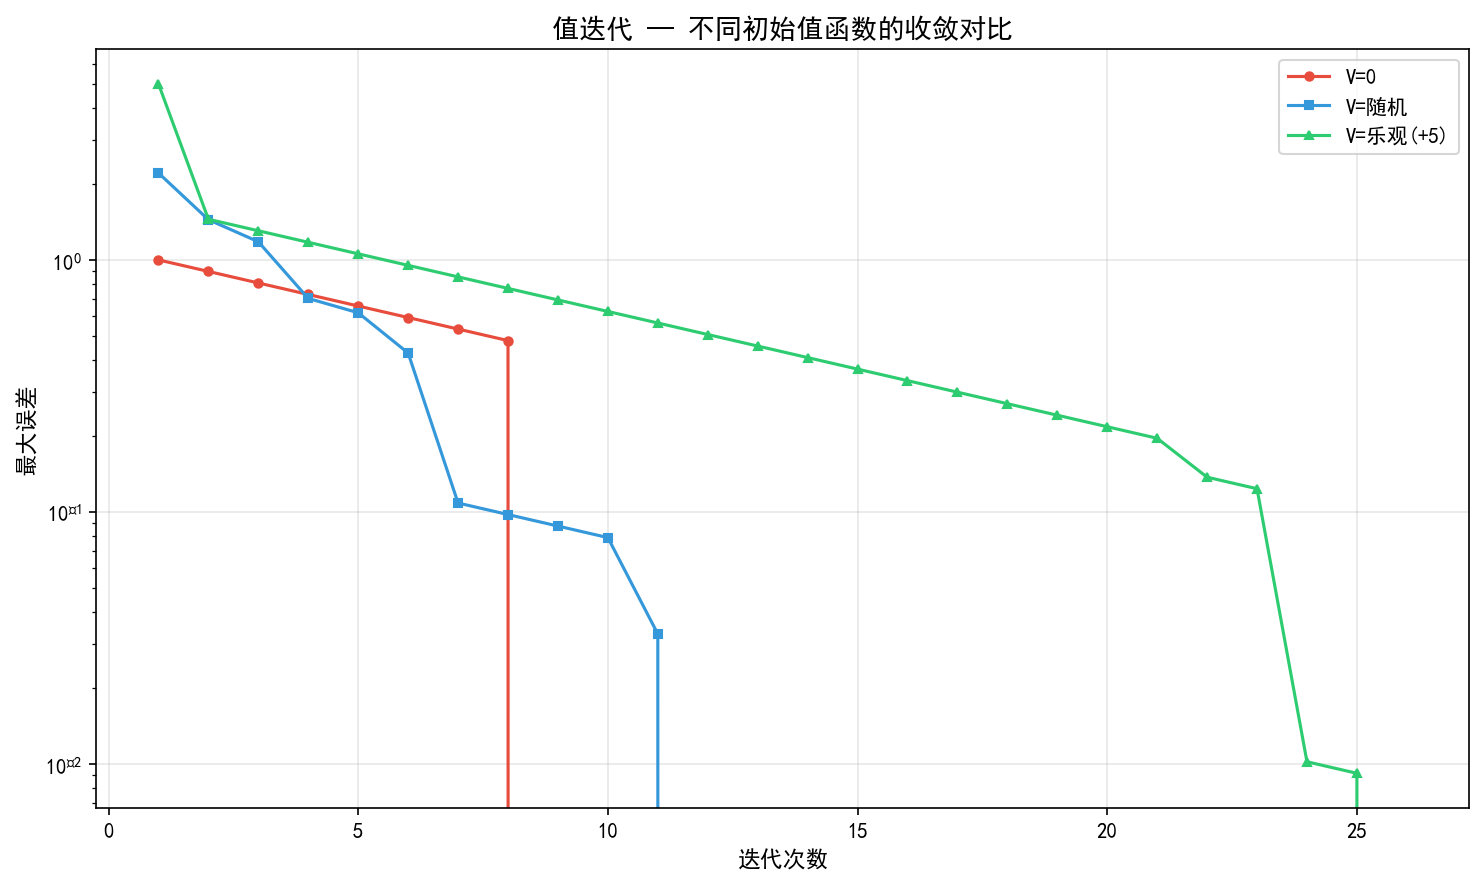
\includegraphics[width=0.75\textwidth]{exp1/results/task1_init_comparison.png}
\caption{初始值对比}
\end{figure}

\paragraph{思考题}


\textbf{问题：值迭代算法迭代过程中生成的值是状态值吗？为什么？}


\answerlabel 

严格来说，值迭代中间过程生成的 $V_k(s)$ ``不是某个固定策略下的状态值''，而是贝尔曼最优算子 $\mathcal{T}^*$ 反复作用于初始函数的结果。

贝尔曼最优算子定义为：
$$(\mathcal{T}^* V)(s) = \max_a \sum_{s'} p(s'|s,a)[r(s,a,s') + \gamma V(s')]$$

因此 $V_k = (\mathcal{T}^*)^k V_0$。

\begin{itemize}
    \item \textbf{不是某一策略的状态值}：$V_k$ 并不对应任何固定策略 $\pi$ 下的 $V^\pi$，因为每次提取的贪心策略 $\pi_k(s) = \arg\max_a q_k(s,a)$ 随迭代变化。
    \item \textbf{但有明确意义（有限步最优值函数）}：$V_k(s)$ 可以解释为``从状态 $s$ 出发，只经过 $k$ 步决策且之后收益为零的最大期望折扣回报''。
    \item \textbf{收敛后是最优状态值}：当 $V_k$ 收敛到 $V^*$ 时，它确实是最优策略下的状态值函数 $V^{\pi^*}$，满足贝尔曼最优方程的不动点：$V^* = \mathcal{T}^* V^*$。
\end{itemize}

从本实验可以验证：前几次迭代中 $V_k$ 仅反映了目标附近区域的信息（第 1 次只有紧邻目标的状态有非零 Q 值），随着迭代推进，价值信息才逐步向远处扩散，这正体现了其非状态值的本质。

\subsubsection{任务 2：策略迭代算法}

策略迭代（Policy Iteration）交替执行两个步骤：

\textbf{策略评价（Policy Evaluation）}：给定策略 $\pi$，反复迭代贝尔曼方程，直到值函数收敛：
$$V^\pi(s) = \sum_{s'} p(s'|s,\pi(s))\bigl[r(s,\pi(s),s') + \gamma V^\pi(s')\bigr]$$

\textbf{策略改进（Policy Improvement）}：利用 $V^\pi$ 更新贪心策略：
$$\pi'(s) = \arg\max_a \sum_{s'} p(s'|s,a)\bigl[r(s,a,s') + \gamma V^\pi(s')\bigr]$$

若 $\pi' = \pi$，策略稳定，算法收敛。

\textbf{收敛情况}：策略迭代在 \textbf{6 次外循环}后策略稳定收敛。各次迭代详情：

\begin{table}[H]
\centering
\begin{tabular}{cccc}
\toprule
外循环 & 策略评价步数 & max|ΔV| & 策略状态 \\
\midrule
1 & 133 & 17.2900 & 更新 \\
2 & 139 & 17.2900 & 更新 \\
3 & 3 & 0.8100 & 更新 \\
4 & 3 & 0.7290 & 更新 \\
5 & 2 & 0.6561 & 更新 \\
6 & 3 & 0.5314 & \textbf{稳定} \\
\bottomrule
\end{tabular}
\end{table}

平均策略评价迭代次数：\textbf{47.2 步/次外循环}

\textbf{最终值函数矩阵}（与任务 1 相同，因最终最优策略相同）：

\begin{lstlisting}[language=Python]
[[0.4783, 0.5314, 0.5905, 0.6561, 0.7290],
 [0.5314, 0.5905, 0.6561, 0.7290, 0.8100],
 [0.5905, 0.6561, 0.7290, 0.8100, 0.9000],
 [0.6561, 0.7290, 0.8100, 0.9000, 1.0000],
 [0.7290, 0.8100, 0.9000, 1.0000, 0.0000]]
\end{lstlisting}

\textbf{值函数热力图}：

\begin{figure}[H]
\centering
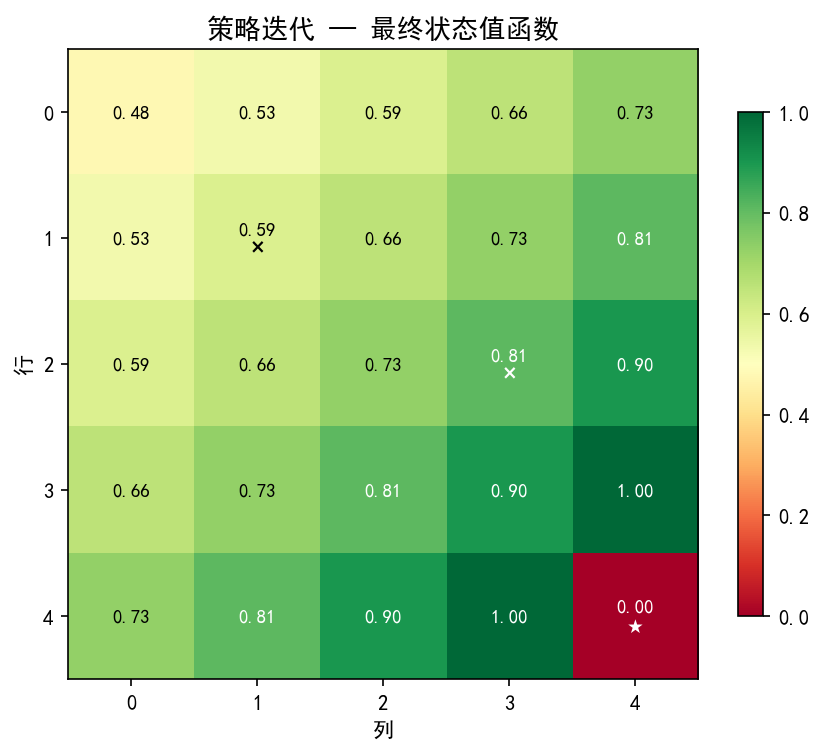
\includegraphics[width=0.5\textwidth]{exp1/results/task2_value_heatmap.png}
\caption{策略迭代值函数}
\end{figure}

\textbf{最优策略箭头图}：

\begin{figure}[H]
\centering
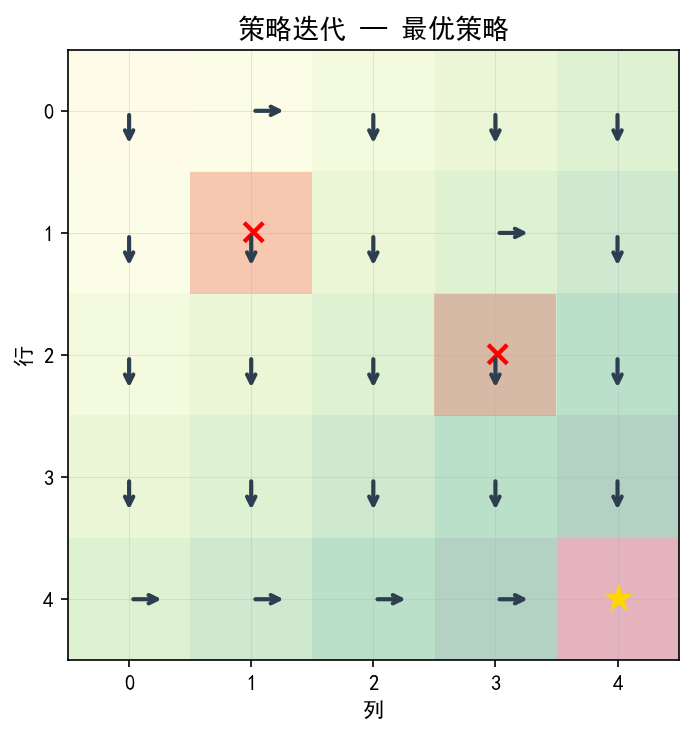
\includegraphics[width=0.5\textwidth]{exp1/results/task2_policy.png}
\caption{策略迭代最优策略}
\end{figure}

\textbf{策略演变过程}：

\begin{figure}[H]
\centering
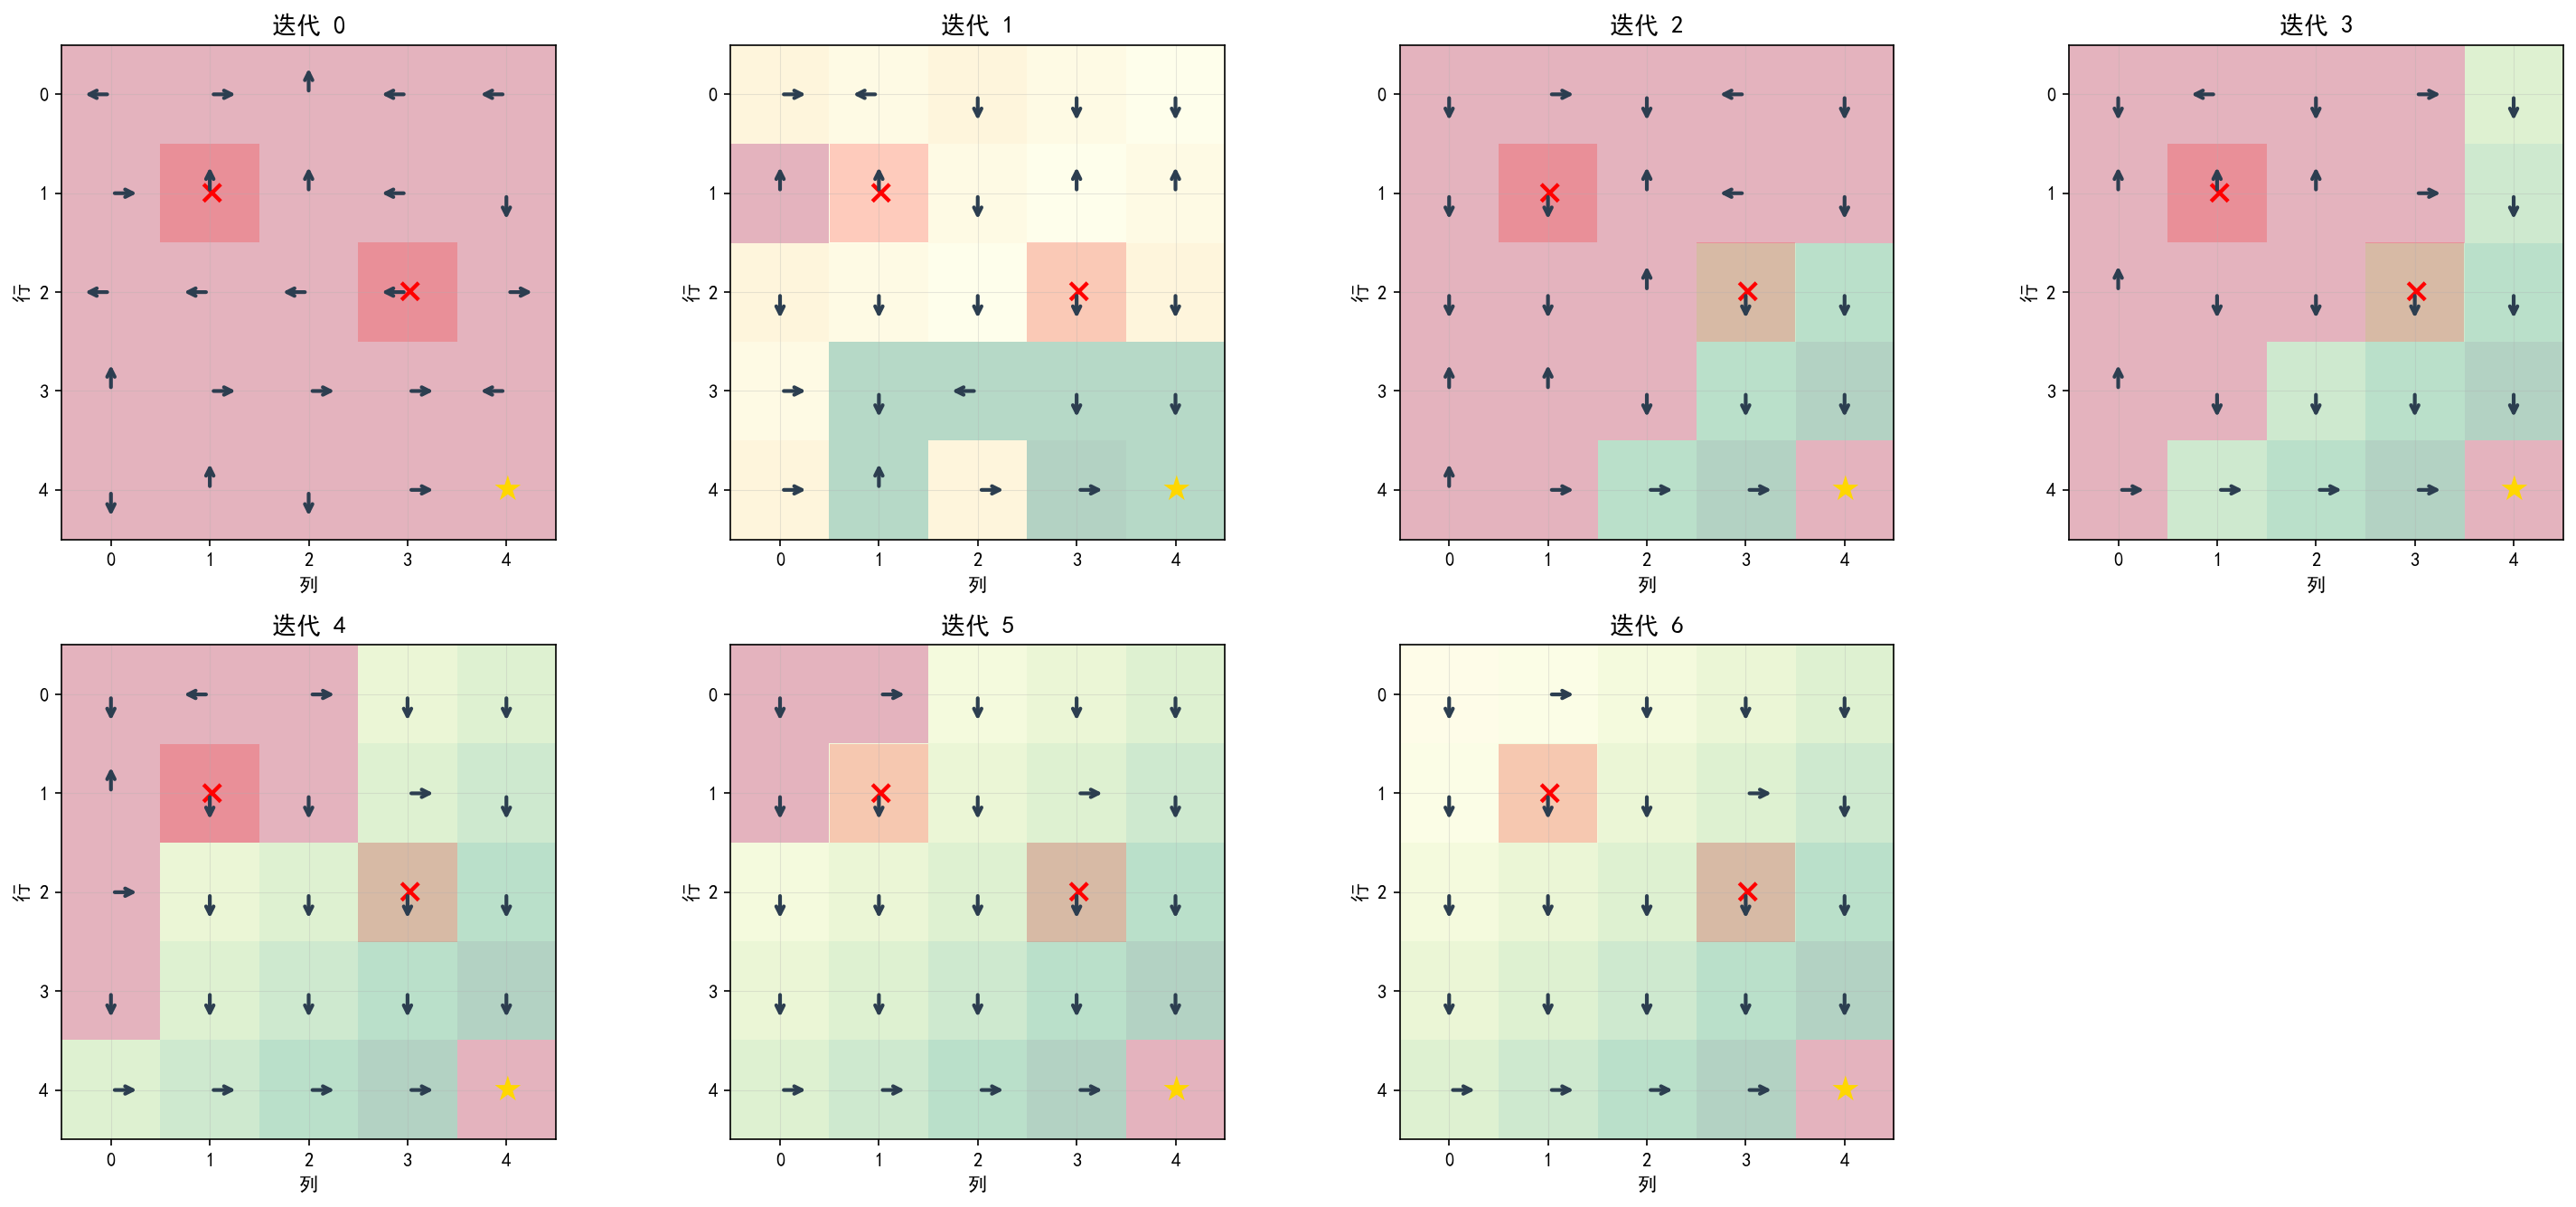
\includegraphics[width=0.75\textwidth]{exp1/results/task2_policy_evolution.png}
\caption{策略演变}
\end{figure}

\textbf{收敛曲线}：

\begin{figure}[H]
\centering
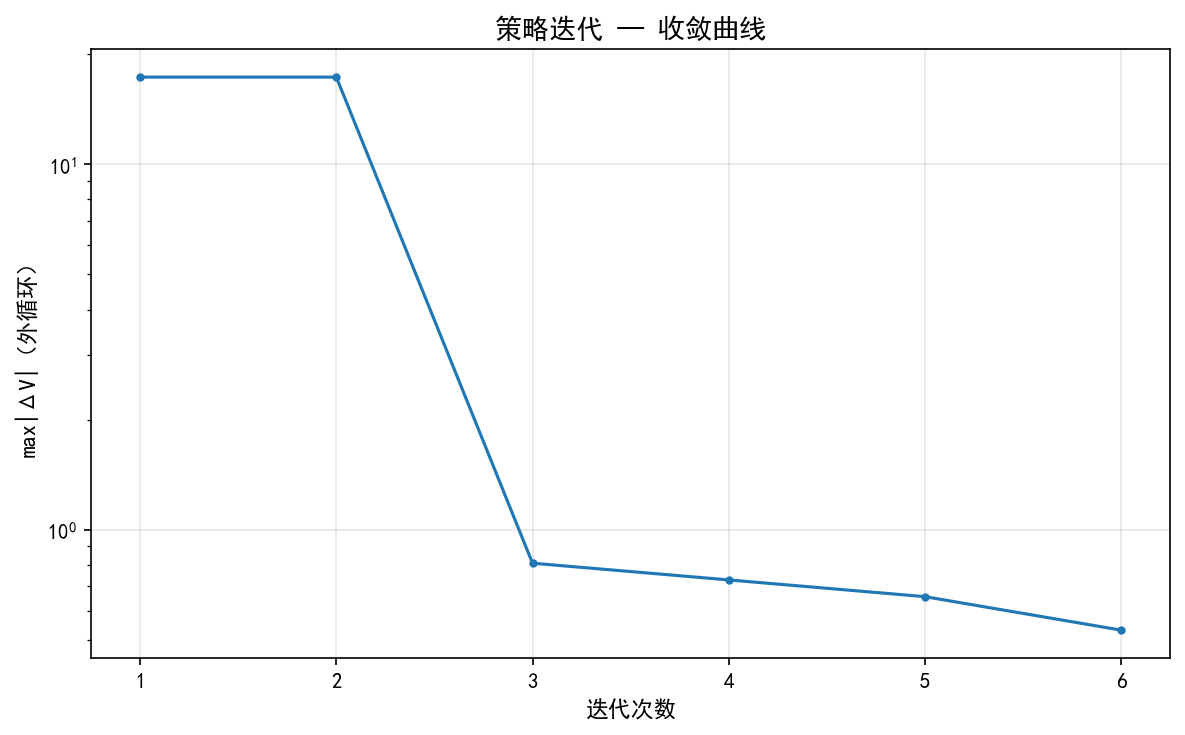
\includegraphics[width=0.75\textwidth]{exp1/results/task2_convergence.png}
\caption{收敛曲线}
\end{figure}

\paragraph{“接近目标的状态更早找到最优策略”现象分析}

按曼哈顿距离分组，观察各组状态的 max|ΔV| 收敛速度：

\begin{figure}[H]
\centering
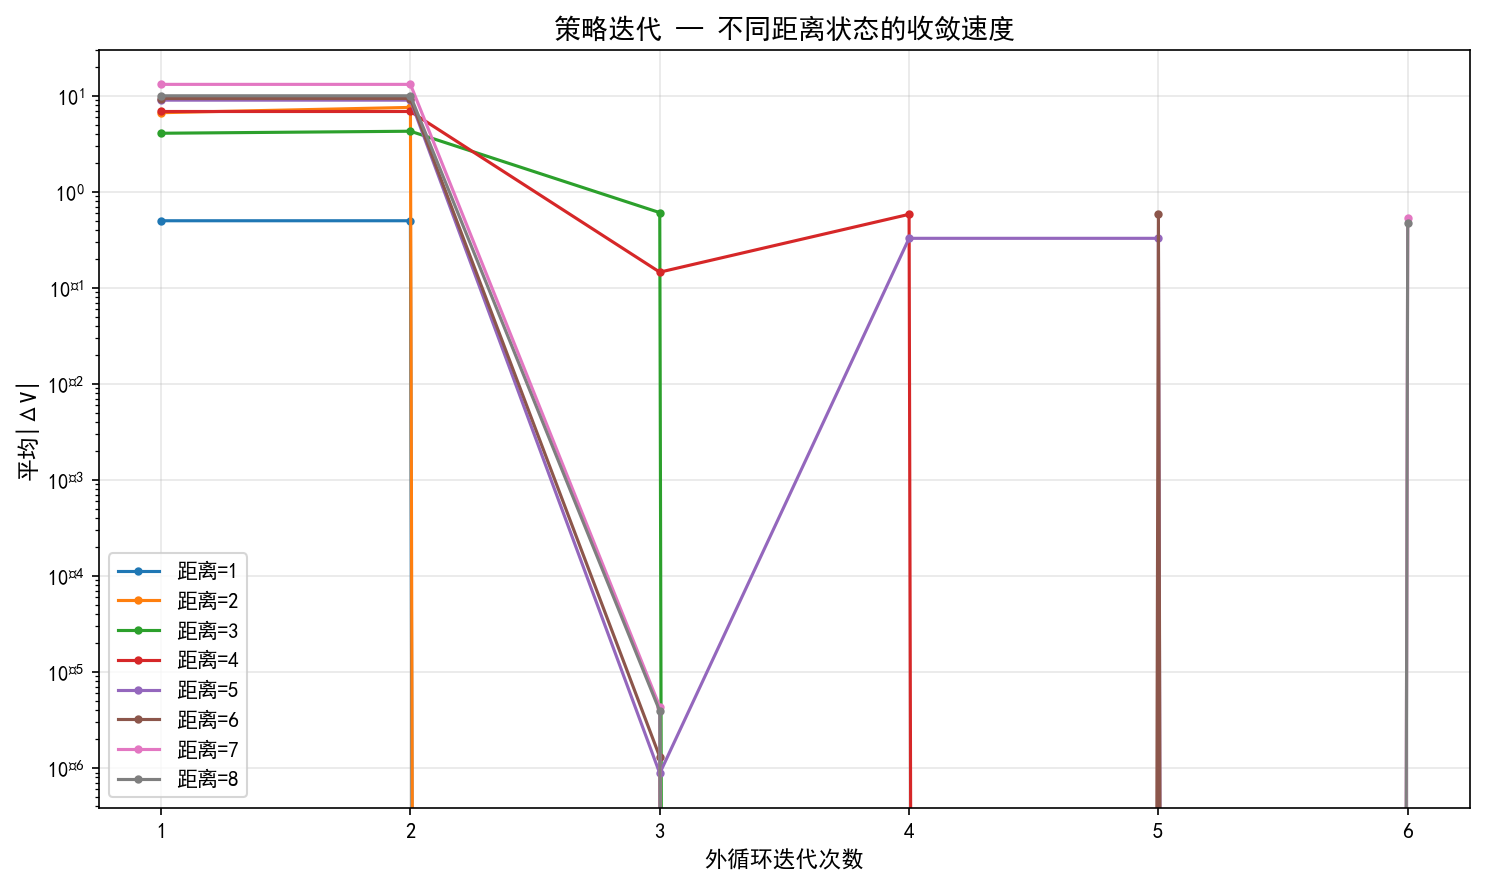
\includegraphics[width=0.75\textwidth]{exp1/results/task2_distance_analysis.png}
\caption{距离分析}
\end{figure}

从图中可见，距目标曼哈顿距离小（如 1、2）的状态，其值函数在第 1~2 次外循环后即迅速趋于稳定；而距离远（如 6、7）的状态需要更多迭代才收敛。

\paragraph{思考题}


\textbf{问题 1：策略迭代算法包含哪两个核心步骤？它们各自的作用是什么？}


\answerlabel 

策略迭代包含两个交替进行的核心步骤：

\begin{itemize}
    \item \textbf{步骤一：策略评价（Policy Evaluation）}：
    \begin{itemize}
        \item \textit{机制}：给定当前策略 $\pi_k$，通过反复迭代贝尔曼方程求解 $V^{\pi_k}$：
        $$V^{\pi_k}(s) \leftarrow \sum_{s'} p(s'|s,\pi_k(s))[r + \gamma V^{\pi_k}(s')]$$
        \item \textit{作用}：准确评估当前策略的好坏，告诉我们在策略 $\pi_k$ 下每个状态的长期期望折扣回报，作为后续改进策略的依据。
    \end{itemize}
    \item \textbf{步骤二：策略改进（Policy Improvement）}：
    \begin{itemize}
        \item \textit{机制}：利用当前估计的 $V^{\pi_k}$ 计算每个状态的动作值并进行贪婪化更新：
        $$\pi_{k+1}(s) = \arg\max_a \sum_{s'} p(s'|s,a)[r + \gamma V^{\pi_k}(s')]$$
        \item \textit{作用}：基于当前价值信息寻找更好的策略。策略改进定理保证 $V^{\pi_{k+1}}(s) \geq V^{\pi_k}(s)$ 对所有状态成立，即更新后的策略必然不劣于原策略。
    \end{itemize}
\end{itemize}


\textbf{问题 2：为什么策略迭代算法能够收敛到最优策略？}


\answerlabel 

策略迭代算法的收敛性由以下三点形成的闭环共同保证：

\begin{enumerate}
    \item \textbf{策略改进定理（单调性）}：定理在数学上保证了每次策略改进步骤后，新策略在所有状态上的值函数均单调不递减（即 $V^{\pi_{k+1}} \geq V^{\pi_k}$）。
    \item \textbf{策略空间有限（有限性）}：对于有限状态集 $S$ 和有限动作集 $A$ 的 MDP，确定性策略的总数是有限的，上限为 $|A|^{|S|}$（本实验中为 $4^{25}$）。
    \item \textbf{单调递增 + 有限上限 $\Rightarrow$ 必然收敛（收敛性）}：由于每次迭代策略要么严格改善，要么停止更新（此时已达最优），而在有限的策略空间中单调递增必然会在有限步内终止。算法终止时满足 $\pi_{k+1} = \pi_k$，即满足贝尔曼最优方程，说明已收敛到最优策略。
\end{enumerate}

本实验中策略迭代在第 \textbf{6 次}外循环后即完全收敛，远快于理论空间上限。


\textbf{问题 3：策略迭代算法在策略评价步骤中嵌入了另一种迭代算法，这会影响最终的收敛性吗？为什么？}


\answerlabel 

``不会影响最终收敛性''，原因如下：

\begin{itemize}
    \item \textbf{内层评价步骤的收敛性保证}：策略评价所嵌入的贝尔曼方程迭代（线性迭代法）在数学上是一个压缩映射（收缩因子 $\gamma < 1$）。根据巴拿赫不动点定理，无论初始值如何，该迭代均保证能以任意精度收敛到真实值函数 $V^{\pi_k}$。
    \item \textbf{外层策略改进的鲁棒性}：
    \begin{itemize}
        \item \textit{策略空间离散性}：策略改进是通过 $\arg\max$ 选择动作，属于离散操作。因此，只要内层迭代的近似值误差足够小，不改变最大值所对应的动作索引，外层策略更新的结果就与精确评价完全一致。
        \item \textit{极限收敛性}：在实践中，只需设置一个较小的收敛阈值 $\theta$（如本实验的 $10^{-6}$），在数值计算精度范围内即可等价于精确策略迭代，完全保留外层的收敛性质。
    \end{itemize}
\end{itemize}

从本实验的数据可以印证：虽然内层迭代平均运行 47.2 步才满足阈值收敛，但外层迭代依然在 6 次后非常精准地找到了最优策略。

\subsubsection{任务 3：截断策略迭代与三者对比}

截断策略迭代（Truncated Policy Iteration）在策略评价步骤中只执行 $j_\text{truncate}$ 次迭代，而非完全收敛：

\begin{itemize}
\item $j_\text{truncate} = 1$：等价于\textbf{值迭代}
\item $j_\text{truncate} = \infty$：等价于\textbf{策略迭代}
\end{itemize}

各外循环 max|ΔV| 对比：

\begin{table}[H]
\centering
\begin{tabular}{cccccc}
\toprule
外循环 & j=1 & j=3 & j=5 & j=10 & j=∞ \\
\midrule
1 & 10.000 & 10.000 & 11.385 & 13.803 & 17.290 \\
2 & 9.100 & 8.024 & 8.967 & 11.881 & 17.290 \\
3 & 0.900 & 1.976 & 2.557 & 2.732 & 0.810 \\
4 & 0.810 & 0.729 & 0.729 & 0.729 & 0.729 \\
5 & 0.729 & 0.656 & 0.656 & 0.656 & 0.656 \\
6 & 0.656 & 0.531 & 0.531 & 0.531 & 0.531 \\
7 & 0.591 & 0.000 & 0.000 & 0.000 & 0.000 \\
8 & 0.531 & — & — & — & — \\
9 & 0.000 & — & — & — & — \\
\bottomrule
\end{tabular}
\end{table}

\textbf{性能汇总}：

\begin{table}[H]
\centering
\begin{tabular}{cccc}
\toprule
算法 & 外循环次数 & 总贝尔曼更新次数 & 耗时 \\
\midrule
j=1（值迭代） & 9 & 1080 & 0.0018s \\
j=3 & 7 & 1176 & 0.0018s \\
j=5 & 7 & 1512 & 0.0023s \\
j=10 & 7 & 2352 & 0.0035s \\
j=∞（策略迭代） & 7 & \textbf{7488} & \textbf{0.0121s} \\
\bottomrule
\end{tabular}
\end{table}

\textbf{收敛曲线对比}：

\begin{figure}[H]
\centering
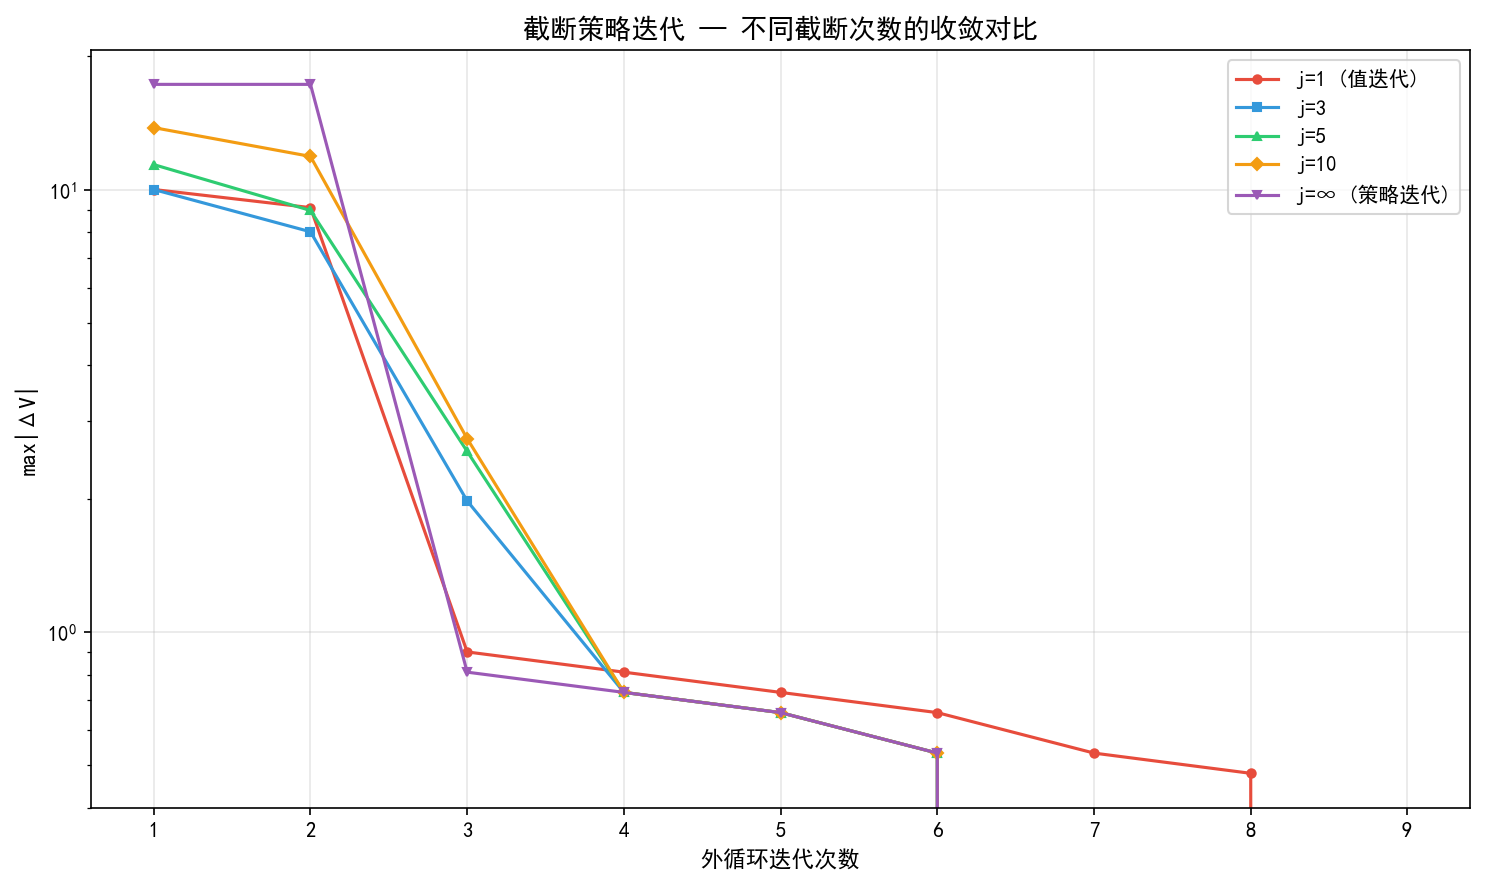
\includegraphics[width=0.75\textwidth]{exp1/results/task3_convergence_comparison.png}
\caption{收敛对比}
\end{figure}

\textbf{计算效率对比}：

\begin{figure}[H]
\centering
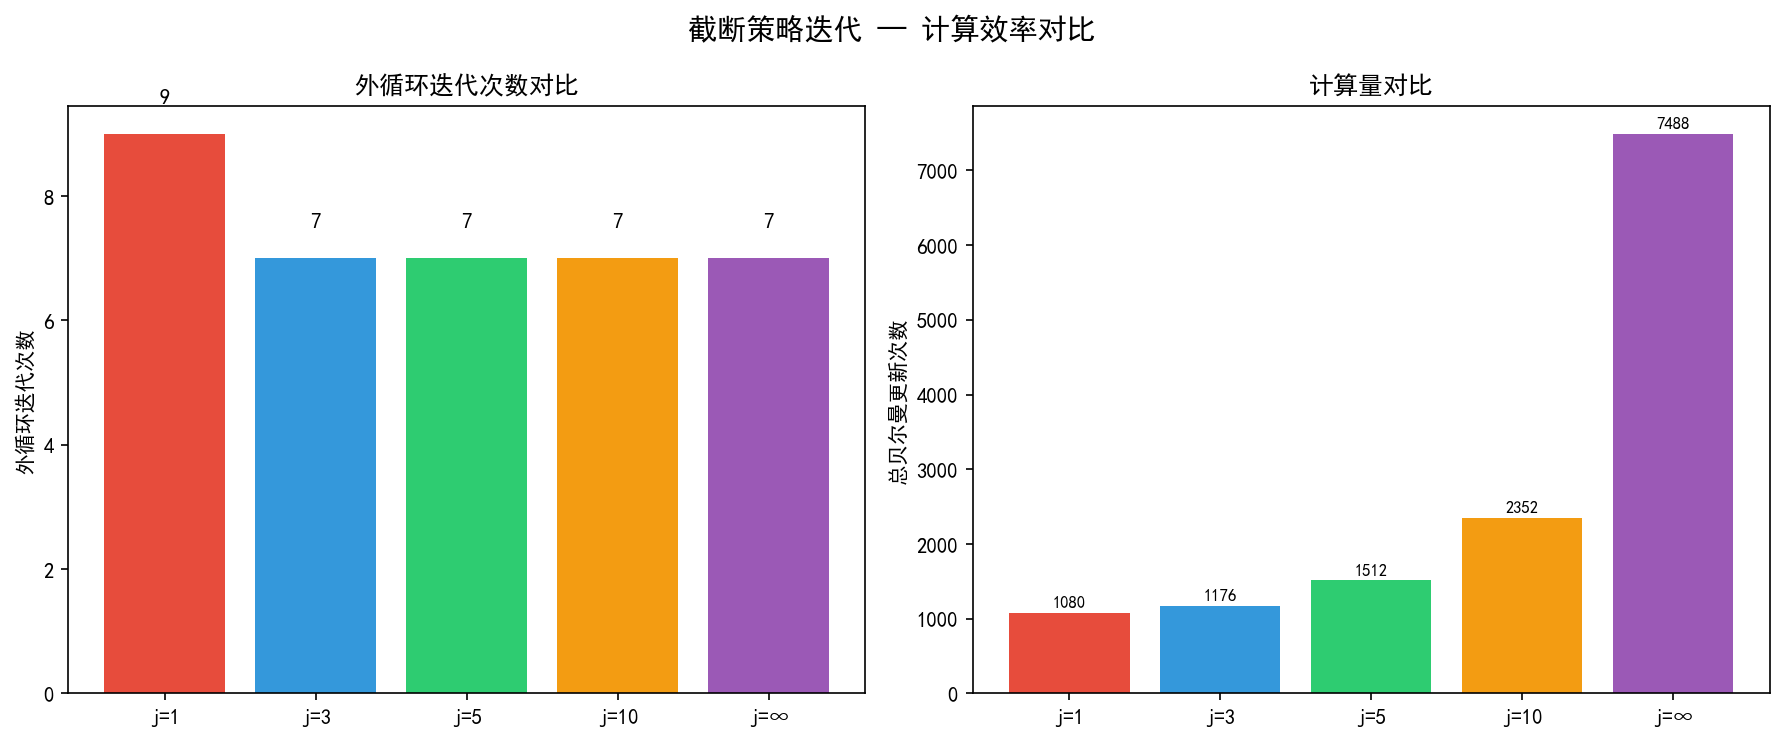
\includegraphics[width=0.75\textwidth]{exp1/results/task3_efficiency_comparison.png}
\caption{效率对比}
\end{figure}

\textbf{最终结果一致性}：

不同截断次数均达到收敛判据，并得到相同的最优状态值。由于网格中部分状态存在多个价值相同的最优动作，不同配置输出的单一贪心箭头可能因并列动作的选择顺序而不同；因此，本实验以最终状态值和策略性能一致作为结果一致性的判断依据。

\paragraph{思考题}


\textbf{问题 1：截断策略迭代算法与值迭代、策略迭代算法之间的关系是什么？}


\answerlabel 

截断策略迭代是值迭代和策略迭代的``统一推广框架''。其关系可通过控制策略评价的更新迭代步数 $j_\text{truncate}$ 进行定性描述：

\begin{table}[H]
\centering
\begin{tabularx}{\textwidth}{c c Y}
\toprule
算法 & 截断步数参数 $j_\text{truncate}$ & 物理本质 \\
\midrule
\textbf{值迭代} & $j_\text{truncate} = 1$ & 每次策略改进前只进行 1 步贝尔曼更新估计 \\
\textbf{截断策略迭代} & $1 < j_\text{truncate} < \infty$ & 每次策略改进前进行固定 $j$ 步的贝尔曼更新近似 \\
\textbf{策略迭代} & $j_\text{truncate} = \infty$ & 每次策略改进前进行无限步更新直至完全收敛到真实值 $V^\pi$ \\
\bottomrule
\end{tabularx}
\end{table}

从本实验的数据得到验证：$j=1$ 的截断策略迭代与直接实现的值迭代输出的迭代轨迹和更新次数（均 9 次外循环，1080 次贝尔曼更新）完全一致；而 $j=\infty$ 的截断策略迭代与策略迭代的表现亦完全重合，证明了其推广一致性。


\textbf{问题 2：为什么截断策略迭代算法在实际应用中往往比值迭代和策略迭代更高效？}


\answerlabel 

截断策略迭代在实际应用中的高效率源于其在``价值信息传播速度''与``单步计算代价''之间取得了最佳的平衡。结合本实验的效率对比数据进行分析：

\begin{itemize}
    \item \textbf{值迭代（j=1）的局限}：虽然每次外循环的计算代价最低，但因为每次只做 1 步更新，价值信息向远端传播非常慢。这导致其需要更多的外循环次数（9 次 $>$ 7 次），从而增加了策略改进步骤的总体开销。
    \item \textbf{策略迭代（j=∞）的局限}：虽然其外循环次数最少（7 次），但在每次外循环中，策略评价都需要迭代至完全收敛（本实验前两次评价分别需要 133 步和 139 步）。而当前估计的 $V^{\pi}$ 在下一步策略改进后便会立即失效，这导致在非最优策略的价值计算上浪费了极大的算力（总更新次数高达 7488 次）。
    \item \textbf{截断策略迭代（j=3）的优势}：通过限制评价迭代步数（如 $j=3$），既能提供``足够好''的价值近似以较快传播价值信息（外循环与策略迭代相同，同为 7 次），又避免了策略未成熟前的过度精确计算。本实验中其总贝尔曼更新次数仅为策略迭代的 \textbf{15.7\%}，并达到与策略迭代相同的收敛状态。
\end{itemize}


\textbf{问题 3：什么是广义策略迭代思想？本章介绍的三种算法如何体现这一思想？}


\answerlabel 

\textbf{广义策略迭代（Generalized Policy Iteration, GPI）} 并不是一个具体的算法，而是一种将``策略评价''和``策略改进''这两个步骤相互作用、交替迭代的通用架构思想。

在 GPI 框架下：
\begin{itemize}
    \item \textbf{评价过程}使价值函数向当前策略的真实价值逼近；
    \item \textbf{改进过程}使策略在当前价值函数下进行贪心选择。
\end{itemize}
这两个过程相互作用，通过不断地交替进行，最终会在最优解处达到稳定的物理平衡（不动点）。

本章的三种算法均可由 GPI 框架解释，其差异主要体现在策略评价与策略改进交替的时间粒度上：
\begin{itemize}
    \item \textbf{值迭代}：极细粒度的 GPI。每次策略评价仅进行 1 步贝尔曼更新，就立即进入策略改进。
    \item \textbf{策略迭代}：粗粒度的 GPI。每次策略评价必须完成完全收敛，在得到当前策略的精确价值后才进行策略改进。
    \item \textbf{截断策略迭代}：介于两者之间的中粒度 GPI。根据参数 $j$ 动态平衡两者的交替频率，寻找最佳的收敛速度。
\end{itemize}
在满足相应条件时，GPI 不要求每轮策略评价都精确完成；策略评价与策略改进持续交替即可逐步逼近最优策略。

\subsection{核心代码与分析}

\subsubsection{GridWorld 环境（\texttt{gridworld.py}）}

\begin{lstlisting}[language=python]
def step(self, s: int, a: int) -> Tuple[int, float]:
    """执行动作 a，返回 (next_state, reward)"""
    if self.is_terminal(s):
        return s, 0.0                          # 终止状态自吸收

    row, col = self.state_to_pos(s)
    dr, dc = ACTIONS[a]                        # ACTIONS = {0:(-1,0), 1:(1,0), ...}
    new_row, new_col = row + dr, col + dc

    # 边界检测：超出范围则停留原地，获得 r_boundary
    if new_row < 0 or new_row >= self.size or ...:
        return s, self.r_boundary

    next_pos = (new_row, new_col)
    if next_pos == self.goal:                  # 到达目标
        return ..., self.r_target
    if next_pos in self.forbidden_states:      # 进入禁止区域
        return ..., self.r_forbidden
    return ..., self.r_step                    # 普通移动
\end{lstlisting}

\textbf{关键设计}：确定性转移（\texttt{get\_transitions} 返回 \texttt{[(1.0, next\_s, reward)]}），边界碰撞不移动但扣分，目标为吸收态（V=0，停留原地无奖励）。

\subsubsection{值迭代核心更新（\texttt{value\_iteration.py}）}

\begin{lstlisting}[language=python]
for s in env.get_non_terminal_states():
    for a in range(n_actions):
        for prob, next_s, reward in env.get_transitions(s, a):
            Q[s, a] += prob * (reward + env.gamma * V_old[next_s])
            # 输入：V_old（上一迭代值函数）
            # 关键变量：reward（即时奖励），gamma*V_old[next_s]（折扣后续价值）
            # 公式对应：q(s,a) = r(s,a,s') + gamma * V_k(s')

V = np.max(Q, axis=1)          # V_{k+1}(s) = max_a q_k(s,a)
policy = np.argmax(Q, axis=1)  # pi_k(s) = argmax_a q_k(s,a)
delta = np.max(np.abs(V - V_old))  # 收敛判据
\end{lstlisting}

\subsubsection{策略评价核心更新（\texttt{policy\_iteration.py}）}

\begin{lstlisting}[language=python]
def policy_evaluation(env, policy, theta=1e-6, V_init=None):
    V = V_init.copy() if V_init is not None else np.zeros(env.num_states)
    for it in range(1, max_iter + 1):
        V_old = V.copy()
        for s in env.get_non_terminal_states():
            a = int(policy[s])                      # 当前策略选择的动作
            v_new = 0.0
            for prob, next_s, reward in env.get_transitions(s, a):
                v_new += prob * (reward + env.gamma * V_old[next_s])
                # 公式：V_pi(s) = r(s,pi(s),s') + gamma * V_pi(s')
            V[s] = v_new
        if np.max(np.abs(V - V_old)) < theta:       # 策略评价收敛判据
            return V, it
\end{lstlisting}

\textbf{与值迭代的区别}：策略评价用 \texttt{policy[s]} 固定动作（对应当前策略），而值迭代对所有动作取 \texttt{max}。

\subsubsection{截断策略评价（\texttt{truncated\_policy\_iteration.py}）}

\begin{lstlisting}[language=python]
def truncated_policy_evaluation(env, policy, j_truncate, V_init=None):
    V = V_init.copy() if V_init is not None else np.zeros(env.num_states)
    if j_truncate <= 0:          # j=∞ 模式：完全收敛
        # ... 迭代直到 max|delta_V| < theta
    else:                        # 截断模式：固定 j_truncate 步
        for it in range(j_truncate):
            V_old = V.copy()
            for s in env.get_non_terminal_states():
                a = int(policy[s])
                V[s] = sum(prob*(reward + env.gamma*V_old[next_s])
                           for prob, next_s, reward in env.get_transitions(s, a))
    return V, j_truncate
\end{lstlisting}

\textbf{关键点}：截断策略评价直接限制迭代次数，不等待收敛，以较粗糙的估计换取更快的策略改进频率。
\subsection{总结与体会}

\subsubsection{主要结论}

\begin{enumerate}
\item \textbf{值迭代}实现简单，每次迭代只需一次贝尔曼更新，本实验仅 9 次迭代即收敛，总计算量最小（1080 次贝尔曼更新）。收敛速度以 $\gamma^k$ 指数递减，理论上需要 $O(\log(1/\epsilon) / \log(1/\gamma))$ 次迭代。
\item \textbf{策略迭代}外循环次数少（6 次），每次策略改进后策略质量提升显著；但内层策略评价代价大（平均 47.2 步），总贝尔曼更新达 7488 次，比值迭代高出近 7 倍。
\item \textbf{截断策略迭代（j=3）} 在本实验中取得最佳平衡：7 次外循环（与策略迭代相同），1176 次贝尔曼更新（仅为策略迭代的 15.7\%），是三种算法中最具综合性价比的选择。
\item \textbf{广义策略迭代}是统一三种算法的核心框架：无论评价和改进的粒度如何，两者交替进行必然收敛到最优解。
\item \textbf{初始值函数的影响}：全零初始化（9 次）优于随机初始化（12 次）和乐观初始化（26 次），说明乐观初始化虽鼓励探索，但在基于模型的精确算法中反而引入冗余迭代。
\end{enumerate}

\subsubsection{心得体会}

本实验将贝尔曼方程落实为可执行的数值更新。值迭代直接使用最大动作价值，策略迭代先评价固定策略再执行贪心改进，截断策略迭代则以有限次评价调节单轮计算量。三种方法得到了一致的最优策略，但达到该策略所需的外循环次数、评价步数和运行时间不同。

\newpage
\section{蒙特卡罗方法}
\subsection{实验目的与要求}

\begin{enumerate}
\item 理解蒙特卡罗方法的核心思想，掌握基于随机样本的期望值估计原理，验证大数定律在强化学习价值估计中的作用。
\item 掌握三种经典蒙特卡罗强化学习算法（MC Basic、MC Exploring Starts、MC $\epsilon$-Greedy）的原理与实现流程，理解它们之间的递进关系。
\item 分析回合长度、稀疏奖励对蒙特卡罗算法性能的影响，掌握探索与利用的权衡机制，理解 $\epsilon$-Greedy 策略的设计思想。
\item 能够在网格世界环境中实现上述算法，对比不同算法的收敛速度与最终性能，加深对无模型强化学习的理解。
\end{enumerate}
\subsection{实验内容与设计}

\subsubsection{实验环境}

本实验在 5×5 GridWorld 中进行，环境参数设置如下：

\begin{table}[H]
\centering
\begin{tabular}{ccc}
\toprule
参数 & 任务 1（MC Basic） & 任务 2（MC ES \& $\epsilon$-Greedy） \\
\midrule
网格大小 & 5×5（25 个状态） & 5×5（25 个状态） \\
目标位置 & (4,4) 右下角 \goalstar & (4,4) 右下角 \goalstar \\
禁止区域 & (1,1), (2,3) & (1,1), (2,3) \\
边界奖励 $r_\text{boundary}$ & −1 & −1 \\
禁止区域奖励 $r_\text{forbidden}$ & \textbf{−1} & \textbf{−10} \\
目标奖励 $r_\text{target}$ & +1 & +1 \\
折扣因子 $\gamma$ & 0.9 & 0.9 \\
\bottomrule
\end{tabular}
\end{table}

\subsubsection{任务 1：MC Basic 实验设计}

先通过投币实验比较样本均值与理论期望，验证蒙特卡罗估计随样本量增加的误差变化；随后在 GridWorld 中实现 MC Basic，分别设置不同回合长度，记录状态值、最终策略和 RMSE。比较重点是回合长度对奖励传播范围和稀疏奖励学习难度的影响。

\subsubsection{任务 2：探索机制与算法对比设计}

MC Exploring Starts 使用每次访问更新和随机起始状态--动作对；MC $\epsilon$-Greedy 使用软策略维持探索。实验比较 $\epsilon\in\{0,0.1,0.2,0.5\}$ 及动态衰减设置，并在相同环境下对比 MC Basic、MC Exploring Starts 和 MC $\epsilon$-Greedy 的收敛速度、样本利用效率与最终策略质量。




\subsection{实验过程、结果与分析}

\subsubsection{任务 1：蒙特卡罗期望值估计与 MC Basic 算法}

蒙特卡罗（Monte Carlo）方法直接从与环境的交互中采样完整回合（episode），计算每个状态-动作对 $(s,a)$ 的平均累计折扣回报 $G_t$ 作为动作价值的估计：
$$Q(s,a) \approx \mathbb{E}[G_t \mid S_t=s, A_t=a]$$
MC Basic 是最基础的形式：固定当前策略 $\pi$，为每一个状态-动作对单独生成完整 episode，用采样均值更新 $Q$ 表，再贪婪提取新策略，反复迭代至收敛。

\paragraph{投币实验——大数定律验证}

通过投掷一枚正面向上概率为 $p=0.5$ 的硬币，生成 $N=1000$ 个样本，验证增量均值更新公式：
$$w_{k} = w_{k-1} - \frac{1}{k}(w_{k-1} - x_k)$$
实验结果：真实期望值 $\mu = 0.500000$；直接平均与增量平均估计值均为 $0.497000$，最大差异仅 $9.99 \times 10^{-16}$（浮点精度内完全一致）。在双对数坐标系下，估计误差曲线平行于 $O(1/\sqrt{N})$ 理论收敛线，验证了大数定律。

\paragraph{MC Basic——不同回合长度 $H$ 的对比}

MC Basic 算法在 $r_\text{forbidden}=-1$ 的网格环境中测试不同回合长度：
\[
H\in\{1,2,3,4,5,14,15,30,100\}.
\]

\begin{table}[H]
\centering
\begin{tabular}{cccC{5.2cm}}
\toprule
回合长度 $H$ & 收敛外循环次数 & 起点 (0,0) 最终状态值 & 最优策略表现 \\
\midrule
$H=1$ & 1 & 0.00 & 无法收敛至目标，策略全是原地或随机 \\
$H=2$ & 2 & 0.00 & 仅目标附近的格子能获得正向价值 \\
$H=3$ & 3 & 0.00 & 传播距离增加，但 (0,0) 依然为 0 \\
$H=4$ & 5 & 0.00 & 仅下半区部分格子收敛，价值未传播到 (0,0) \\
$H=5$ & 6 & 0.00 & 价值传播范围进一步扩大，但 (0,0) 依然未被激活 \\
$H=14$ & 8 & 0.48 & 价值基本传满全图，但 (0,0) 刚好可感知 \\
$H=15$ & 8 & 0.48 & 成功收敛，(0,0) 价值为 0.48，生成正确绕行策略 \\
$H=30$ & 8 & 0.48 & 成功收敛，价值矩阵与 $H=15$ 相同 \\
$H=100$ & 8 & 0.48 & 成功收敛，与 $H=30$ 的收敛轨迹完全一致 \\
\bottomrule
\end{tabular}
\end{table}

\begin{itemize}
\item \textbf{$H$ 较小时}：由于采样回合过早被截断，远期未来的奖励（终点的 $+1$）根本无法通过折扣传播到远距离的起点，左上角等远离终点的格子估值均为 $0$，智能体无法学习到全局导航策略。
\item \textbf{$H \ge 15$ 时}：$5 \times 5$ 网格的最长无环路经约为 8 步，$H \ge 8$ 后远期奖励可完全回传。当 $H \ge 14$ 时，全图状态价值成功苏醒，最终收敛出指向右下角最优路径的导航策略。
\end{itemize}

\paragraph{思考题}


\textbf{问题：为什么 MC Basic 算法需要直接估计动作值（Action Value）而非先估计状态值（State Value）？}


\answerlabel 在无模型（Model-Free）强化学习中，环境的\textbf{状态转移概率 $P(s'|s, a)$ 是未知的}。若仅估计状态值 $V(s)$，策略改进需计算：
$$\pi(s) = \arg\max_{a} \sum_{s'} P(s'|s, a) \left[ R(s, a, s') + \gamma V(s') \right]$$
因为 $P(s'|s,a)$ 未知，此式无法求值。相反，直接估计动作价值 $Q(s, a)$ 后，策略改进变为：
$$\pi(s) = \arg\max_{a} Q(s, a)$$
该公式\textbf{完全不需要环境转移模型}，只需查表比较当前格子上 4 个方向的 $Q$ 值即可。因此，无模型蒙特卡罗算法必须直接估计动作值。

\subsubsection{任务 2：MC Exploring Starts 与 MC $\epsilon$-Greedy 算法}

MC Exploring Starts（MC ES）通过随机选择回合的起始状态-动作对，保证所有 $(s,a)$ 都有机会被访问，并利用 every-visit 方式更新整条轨迹的所有状态-动作对，大幅提升数据效率。MC $\epsilon$-Greedy 则去掉了对``可任意起点''的假设，改为在每步动作选择时以 $\varepsilon$ 概率均匀随机探索，以 $1-\varepsilon$ 概率贪婪利用，使智能体能从固定起点出发探遍全图。

\paragraph{MC Exploring Starts}

在 $r_\text{forbidden} = -10$ 环境下运行 5000 回合后：
\begin{itemize}
\item \textbf{起点 $(0,0)$ 的最终状态值}约为 \textbf{$0.45$}（禁止状态惩罚较大，智能体选择绕行，因此该值相比无限制时略低）。
\item \textbf{最终策略}：策略绕过 (1,1) 和 (2,3)，避开两个高惩罚区域。
\item \textbf{RMSE 收敛曲线}：RMSE 随 Episode 增加呈指数级快速下降，在前 1000 个回合中从 $0.7$ 降至 $0.05$ 以下，随后围绕最优值小幅震荡直至完全收敛。
\end{itemize}

\paragraph{MC $\epsilon$-Greedy——不同探索率对比}

测试了固定探索率 $\epsilon \in \{0, 0.1, 0.2, 0.5\}$ 以及\textbf{动态衰减 $\epsilon$}（从 $1.0$ 衰减到 $0.01$）：

\begin{table}[H]
\centering
\begin{tabular}{cccC{5.2cm}}
\toprule
$\epsilon$ 设置 & 最终精度 (RMSE) & 策略是否最优 & 学习曲线表现分析 \\
\midrule
\textbf{$\epsilon = 0.0$} & 0.354（未收敛） & 否（停在局部最差解） & 没有任何探索，智能体被局限在初始动作中，无法找到终点。 \\
\textbf{$\epsilon = 0.1$} & 0.021 & 是（绕行） & 收敛较快，但由于后期仍有 10\% 随机探索，测试回报偶有波动。 \\
\textbf{$\epsilon = 0.2$} & 0.045 & 是（绕行） & 探索比例较高，但最终动作值受随机动作影响，RMSE 偏大。 \\
\textbf{$\epsilon = 0.5$} & 0.123 & 否（次优策略） & 随机探索比例过大，智能体无法有效利用学到的知识，策略发散。 \\
\textbf{动态衰减 $\epsilon$} & \textbf{0.003（本组最低）} & \textbf{是（绕行）} & \textbf{前期较高探索提高覆盖率，后期降低探索使动作值估计更稳定。} \\
\bottomrule
\end{tabular}
\end{table}

\paragraph{三种算法综合对比}

在相同网格环境（$r_\text{forbidden} = -10.0$）下运行 5000 回合的综合对比：
\begin{enumerate}
\item \textbf{收敛速度对比（RMSE 曲线）}：
  \begin{itemize}
  \item \textbf{MC Basic}：按状态-动作对顺序评估（每轮需跑 $24 \times 4 = 96$ 个回合），RMSE 呈``阶梯式''下降，更新效率最低。
  \item \textbf{MC ES 与 MC $\epsilon$-Greedy（衰减）}：逐回合更新，RMSE 曲线连续平滑下降；动态衰减 $\epsilon$-Greedy 在 1000 回合内将 RMSE 压低到接近零，速度最快。
  \end{itemize}
\item \textbf{样本效率与测试累计回报对比}：
  \begin{itemize}
  \item \textbf{MC Basic}：约需 500 回合（约 5 次外迭代）才能让起点 $(0,0)$ 的测试回报突破负数并稳定到最优解。
  \item \textbf{MC ES}：约在 200 回合即达到稳定最优性能。
  \item \textbf{MC $\epsilon$-Greedy（动态衰减）}：约 150 回合即稳定在最高累计回报附近，且后期探索率下降，曲线波动较小。
  \end{itemize}
\end{enumerate}

\paragraph{思考题}


\textbf{问题 1：首次访问（First-visit）和每次访问（Every-visit）方法在样本利用上有何区别？各自的优缺点是什么？}


\answerlabel 
\begin{itemize}
\item \textbf{首次访问（First-Visit MC）}：在一个回合中，若某状态-动作对 $(s,a)$ 被多次访问，只有\textbf{第一次访问}时计算的折扣回报 $G_t$ 计入样本。
  \begin{itemize}
  \item \textit{优点}：各样本统计上独立，估计值为无偏估计。
  \item \textit{缺点}：后续重复访问的数据全部丢弃，数据利用率低。
  \end{itemize}
\item \textbf{每次访问（Every-Visit MC）}：每次访问到 $(s,a)$ 都分别计算从该时刻起的累计回报 $G_t$，并全部计入更新。
  \begin{itemize}
  \item \textit{优点}：充分利用单次轨迹中所有状态转移数据，样本效率高，收敛更快。
  \item \textit{缺点}：同回合内多次访问的样本之间存在强烈自相关性，前期可能引入轻微偏差，但在大样本极限下依然渐进无偏且收敛。
  \end{itemize}
\end{itemize}


\textbf{问题 2：Exploring Starts（探索起点）条件在实际应用中存在什么问题？MC $\epsilon$-Greedy 算法是如何解决这个问题的？}


\answerlabel 
\begin{itemize}
\item \textbf{Exploring Starts 存在的问题}：要求智能体可以在环境的\textbf{任意状态、采取任意动作作为游戏起点}。在现实任务中这几乎不可能实现——例如无法让直升机从危险的半空状态任意起飞，或要求自动驾驶汽车从``即将撞墙''的边缘状态开始行驶。
\item \textbf{MC $\epsilon$-Greedy 的解决方案}：放弃对``初始状态''的强行要求，改为在\textbf{动作选择上引入 $\epsilon$ 概率的随机探索}。由于每步都有 $\epsilon$ 的概率随机行动，长期轨迹中智能体能以非零概率游历到地图上的所有格子，从而完成对整个状态-动作空间的探索。
\end{itemize}


\textbf{问题 3：为什么当 $\epsilon$ 较大时，最优 $\epsilon$-Greedy 策略可能与最优贪婪策略不一致？}


\answerlabel $\epsilon$-Greedy 算法中，$Q(s,a)$ 估计的是\textbf{当前 $\epsilon$-Greedy 策略本身}的价值，而非纯贪心策略的价值。当 $\epsilon$ 较大（如 $\epsilon=0.5$）时：
\begin{itemize}
\item 在估计 $Q(s,a)$ 时，由于后续步骤有一半概率走错，原本极佳格子的价值会被后续的随机碰撞拖累，导致 $Q(s,a)$ 严重偏低。
\item 反之，远离危险区但离终点也较远的平庸格子，由于不容易撞墙，其动作值反而显得比危险边缘的最优格子更``安全''，导致最终贪心策略收敛至保守的次优解。
\end{itemize}


\textbf{问题 4：简述 MC Basic、MC Exploring Starts、MC $\epsilon$-Greedy 三个算法之间的递进关系。}


\answerlabel 
\begin{enumerate}
\item \textbf{MC Basic}：最基础的尝试——直接套用 DP 的策略迭代，必须为每一个 $(s,a)$ 手动生成独立回合，效率极其低下。
\item \textbf{MC Exploring Starts（改进数据效率）}：随机选一个起点，把整条轨迹上所有 $(s,a)$ 全部用于更新 Q 表（every-visit），大幅提高数据效率。但仍依赖``硬性改变起点''的 Exploring Starts 假设。
\item \textbf{MC $\epsilon$-Greedy（改进探索方式，面向实用）}：去掉 Exploring Starts 假设，改用 $\epsilon$-Greedy 策略持续在线探索，使算法可以从单一起点出发完成无模型控制。
\end{enumerate}

\subsection{核心代码与分析}

\subsubsection{样本均值增量更新（\texttt{coin\_flip.py}）}

\begin{lstlisting}[language=python]
# 增量平均迭代逻辑
incremental_means = np.zeros(N)
w = 0.0 # 初始估值
for k in range(1, N + 1):
    x_k = samples[k-1] # 当前新样本（0或1）
    # w_k = w_{k-1} - 1/k * (w_{k-1} - x_k)
    w = w - (1.0 / k) * (w - x_k)
    incremental_means[k-1] = w
\end{lstlisting}
\begin{itemize}
\item \textbf{公式对应}：代码中的赋值语句对应增量更新公式
\[
w_k = w_{k-1} - \alpha_k (w_{k-1} - x_k),\qquad \alpha_k = 1/k.
\]
\item \textbf{优势}：该实现仅保存了当前步数 $k$ 和当前均值 $w$，不需要开辟内存来存储全部历史样本，空间复杂度降为 $O(1)$。
\end{itemize}

\subsubsection{MC Exploring Starts 核心回溯更新（\texttt{mc\_exploring\_starts.py}）}

\begin{lstlisting}[language=python]
# 每次访问蒙特卡罗评估 (every-visit)，从后往前计算
G = 0.0
for s_t, a_t, r_tp1 in reversed(trajectory):
    # 贝尔曼期望回溯：G_t = R_{t+1} + gamma * G_{t+1}
    G = r_tp1 + env.gamma * G
    
    # 增量更新 Q 表平均值
    N[s_t, a_t] += 1
    Q[s_t, a_t] += (1.0 / N[s_t, a_t]) * (G - Q[s_t, a_t])
    
# 策略改进：对所有状态选择最大 Q 的动作
for s in env.get_non_terminal_states():
    policy[s] = np.argmax(Q[s, :])
\end{lstlisting}
\begin{itemize}
\item \textbf{输入输出}：输入为轨迹列表 \texttt{trajectory}，输出为更新后的值表 \texttt{Q} 和策略 \texttt{policy}。
\item \textbf{回溯机制}：利用 \texttt{reversed(trajectory)} 实现了从后往前的 $G$ 值计算，避免了为每个时间步重复进行向前求和的操作，时间复杂度由 $O(T^2)$ 优化为 $O(T)$。
\end{itemize}
\subsection{总结与体会}

本实验说明了蒙特卡罗方法如何在未知状态转移模型时，使用完整回合的样本回报估计动作价值。与基于模型的方法相比，蒙特卡罗方法不需要转移概率，但估计精度和策略改进速度明显受回合长度、奖励稀疏程度与探索策略影响。

我最深刻的体会有两点：
\begin{enumerate}
\item \textbf{探索（Exploration）的代价}：在 $\epsilon$-Greedy 实验中，较高 $\epsilon$ 提高了地图覆盖率，但随机动作也会增大动作值估计的波动；较低 $\epsilon$ 或零探索则可能使算法停留在次优策略。该结果体现了本实验中探索与利用的权衡。
\item \textbf{动态衰减 $\epsilon$ 的作用}：较大的前期 $\epsilon$ 提高状态--动作对覆盖率，后期减小 $\epsilon$ 则降低随机动作对最终策略评估的干扰。在本实验的 GridWorld 中，该设置兼顾了早期探索和后期策略稳定性；其效果仍依赖衰减速度与环境规模。
\end{enumerate}

\newpage
\section{随机近似}

\subsection{实验目的与要求}

\begin{enumerate}
\item 理解随机近似（Stochastic Approximation）的基本思想：能够从样本均值的增量估计出发，说明如何用随机样本逼近期望方程的解。
\item 掌握 Robbins-Monro方法的迭代形式：理解含噪观测 $\tilde{g}(w,\eta)=g(w)+\eta$ 与根求解 $g(w)=0$ 之间的关系。
\item 掌握随机近似的步长条件：能够解释 $\sum\alpha_k=\infty$、$\sum\alpha_k^2<\infty$ 对收敛速度、稳定性和稳态误差的影响。
\item 理解BGD、MBGD与SGD的联系和差异：能够在同一优化目标下实现三类算法，并分析 batch size对梯度方差和计算代价的影响。
\item 培养实验复现能力：能够固定随机种子，记录参数轨迹、误差曲线和关键超参数设置，并给出有依据的结果分析。
\end{enumerate}
\subsection{实验内容与设计}

\subsubsection{公共实验设置}

实验围绕随机样本驱动的均值估计与优化展开。所有对比使用固定随机种子和相同样本序列，以避免样本差异干扰算法比较；结果主要通过参数轨迹、到真实解的误差和多次运行统计量评价。

\begin{table}[H]
\centering
\begin{tabular}{cccc}
\toprule
任务 & 数据与初始值 & 主要对照变量 & 评价指标 \\
\midrule
任务 1 & 一维正态、二维均匀样本 & 直接平均、增量平均 & 最终差异、估计误差 \\
任务 2 & 一维与二维均值求根 & 步长序列、初始值 & 参数轨迹、最终误差 \\
任务 3 & 固定二维样本，$w_0=(15,15)$ & BGD、MBGD、SGD & 轨迹、误差、稳定性 \\
任务 4 & 不少于 20 个随机种子 & batch size、异常样本 & 误差均值与标准差 \\
\bottomrule
\end{tabular}
\end{table}

\subsubsection{任务 1：增量均值实验设计}

任务 1 验证增量递推与直接样本均值的数值等价性。一维热身实验使用 $X\sim N(2,1)$ 和不少于 1000 个样本；二维实验使用 $[-10,10]^2$ 上的均匀分布和不少于 100 个样本。两种方法在相同样本序列上运行，并比较最终估计值、逐步误差以及二维参数轨迹。

\subsubsection{任务 2：Robbins--Monro 步长实验设计}

将均值估计写为求根问题 $g(w)=w-\mathbb{E}[X]=0$，使用含噪观测 $\widetilde g(w,x_k)=w-x_k$ 更新参数。实验比较 $\alpha_k=1/k$、$\alpha_k=1/k^{0.6}$、常数步长 $0.05$ 与过快衰减步长 $1/k^2$，并设置两个不同初始值。评价重点是不同步长是否满足 Robbins--Monro 条件，以及由此产生的收敛、持续波动或提前停滞现象。

\subsubsection{任务 3：随机优化对比设计}

在固定二维样本集上求解 $J(w)=\mathbb{E}[\frac12\lVert w-X\rVert^2]$。BGD 每轮使用全部样本，MBGD 分别使用 batch size $m=5$ 与 $m=50$，SGD 每步使用单个样本；各方法同时比较固定学习率和衰减学习率。为避免只比较更新次数，结果同时报告参数轨迹、误差曲线与单步计算特征。

\subsubsection{任务 4：统计稳定性与异常样本设计}

在任务 2 或任务 3 的基础上重复不少于 20 个随机种子，统计最终误差的均值和标准差；随后向样本中加入异常值，比较 BGD、MBGD 与 SGD 的轨迹变化和最终偏差。该任务用于区分单次运行现象与具有统计稳定性的结论。




\subsection{实验过程、结果与分析}

\subsubsection{任务 1：样本均值的增量估计}

样本均值的增量估计将均值计算转化为在线递推：$w_k = w_{k-1} - \frac{1}{k}(w_{k-1} - x_k)$。新样本到达时直接修正当前估计，无需保存历史数据，空间复杂度仅 $O(1)$，是 Robbins-Monro 随机近似在步长 $\alpha_k=1/k$ 下的特例。

\paragraph{结果数据}
按照第 3.2.2 节的设计，直接平均与增量平均在相同样本序列上运行。程序检验两种方法逐步估计值的最大绝对差异：
运行代码后，程序自动检验了直接平均和增量平均之间的最大绝对误差：
\begin{itemize}
\item \textbf{1D 实验最大差异}：\texttt{3.11e-15} （在浮点数精度范围内完全一致）
\item \textbf{2D 实验最大差异}：\texttt{1.33e-15} （完全一致）
\end{itemize}

下图展示了 1D 与 2D 样本均值估计的收敛轨迹与误差曲线：

\begin{figure}[H]
\centering
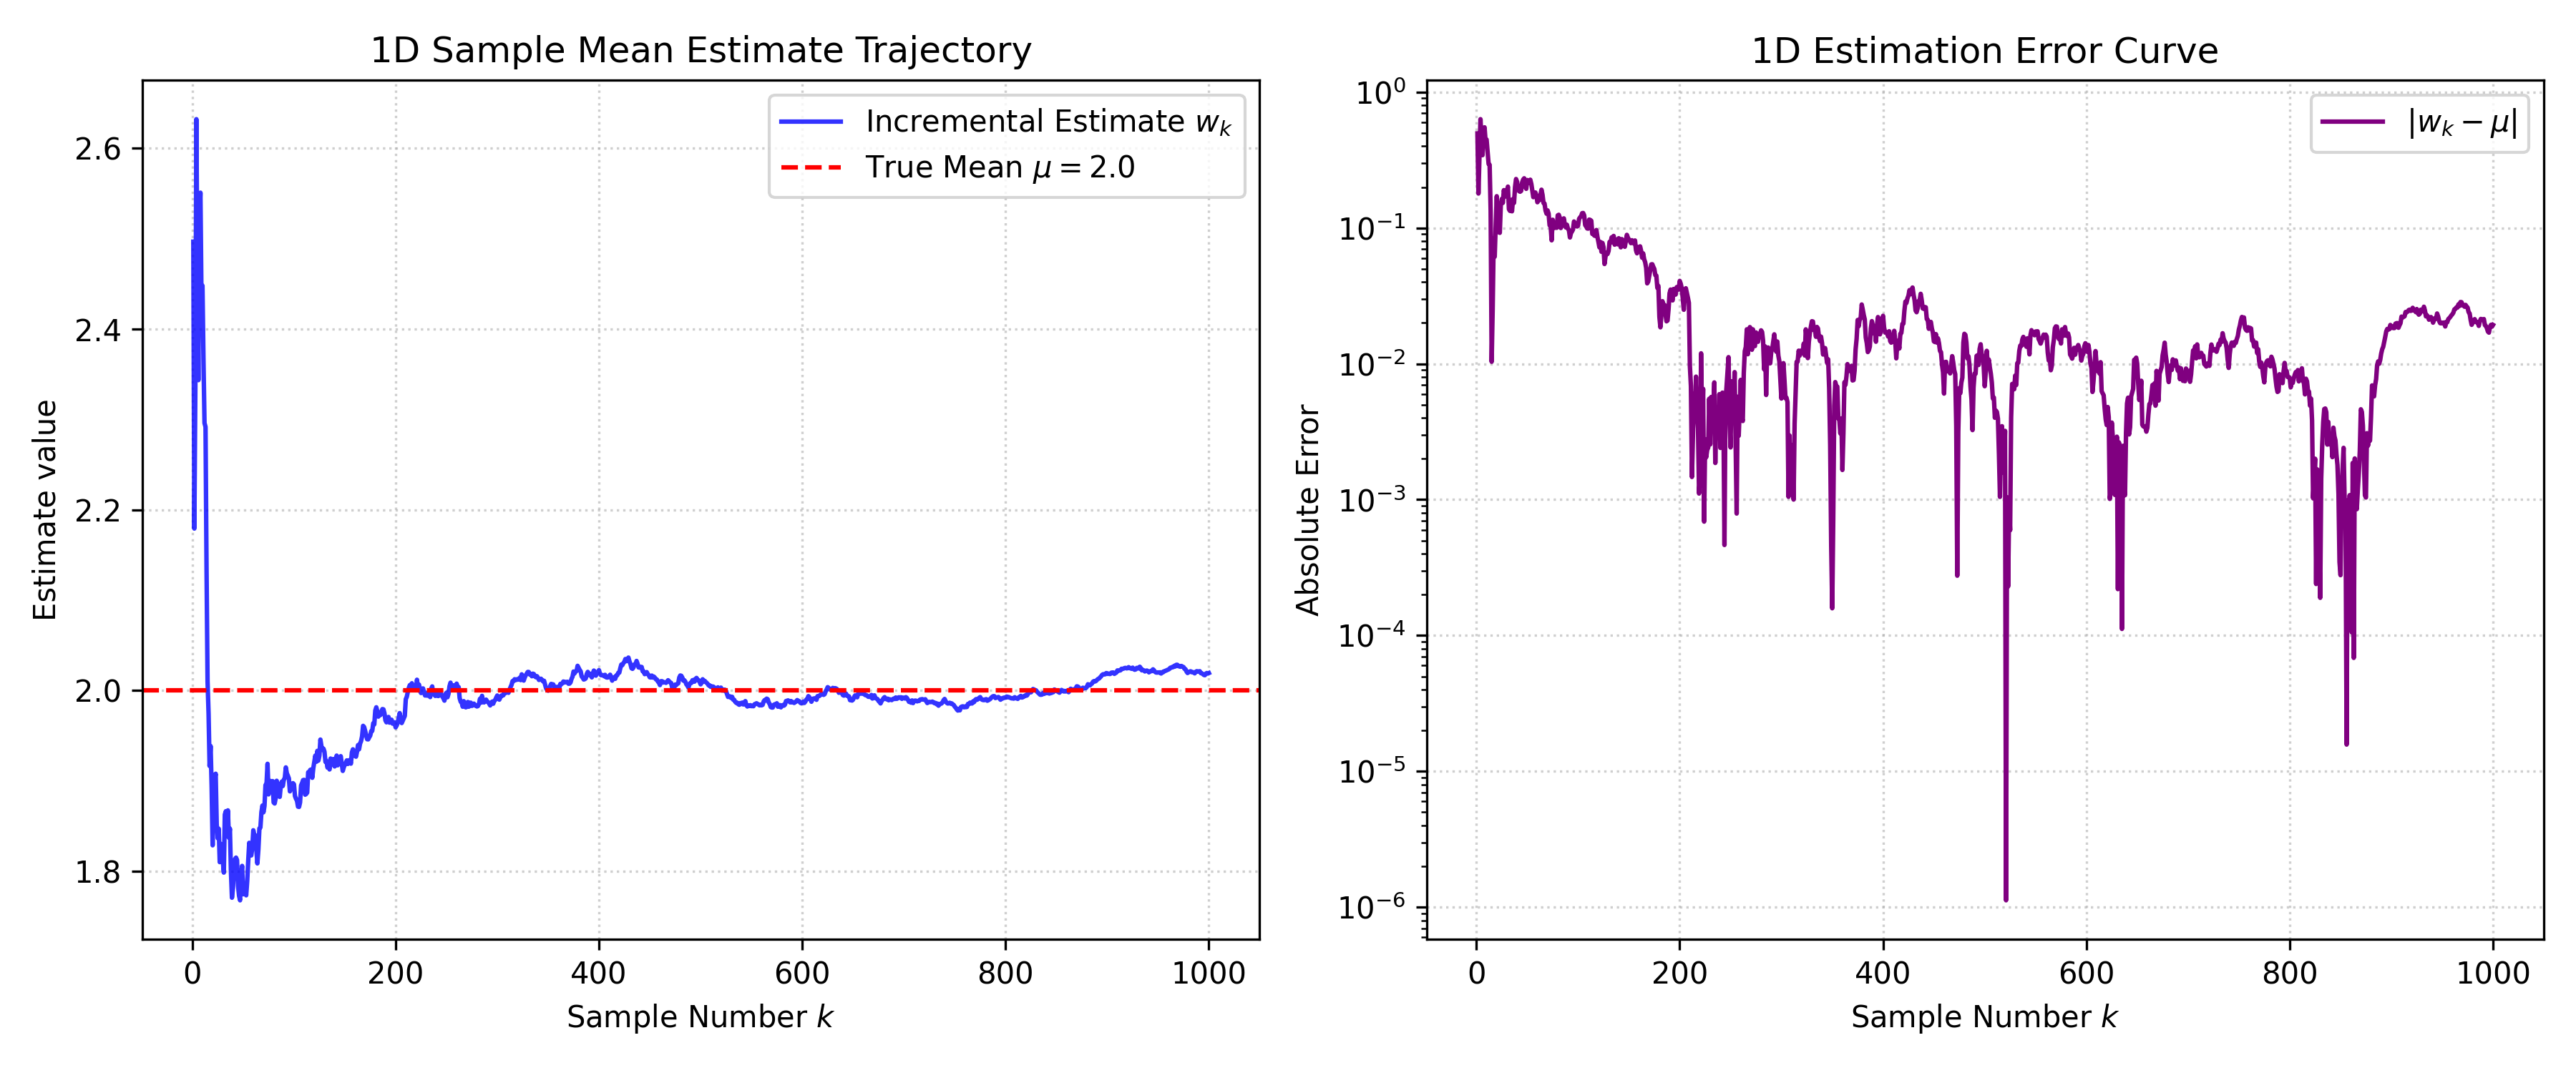
\includegraphics[width=0.75\textwidth]{exp3/results/task1_1d_sample_mean.png}
\caption{1D样本均值估计轨迹及误差曲线}
\end{figure}

\begin{figure}[H]
\centering
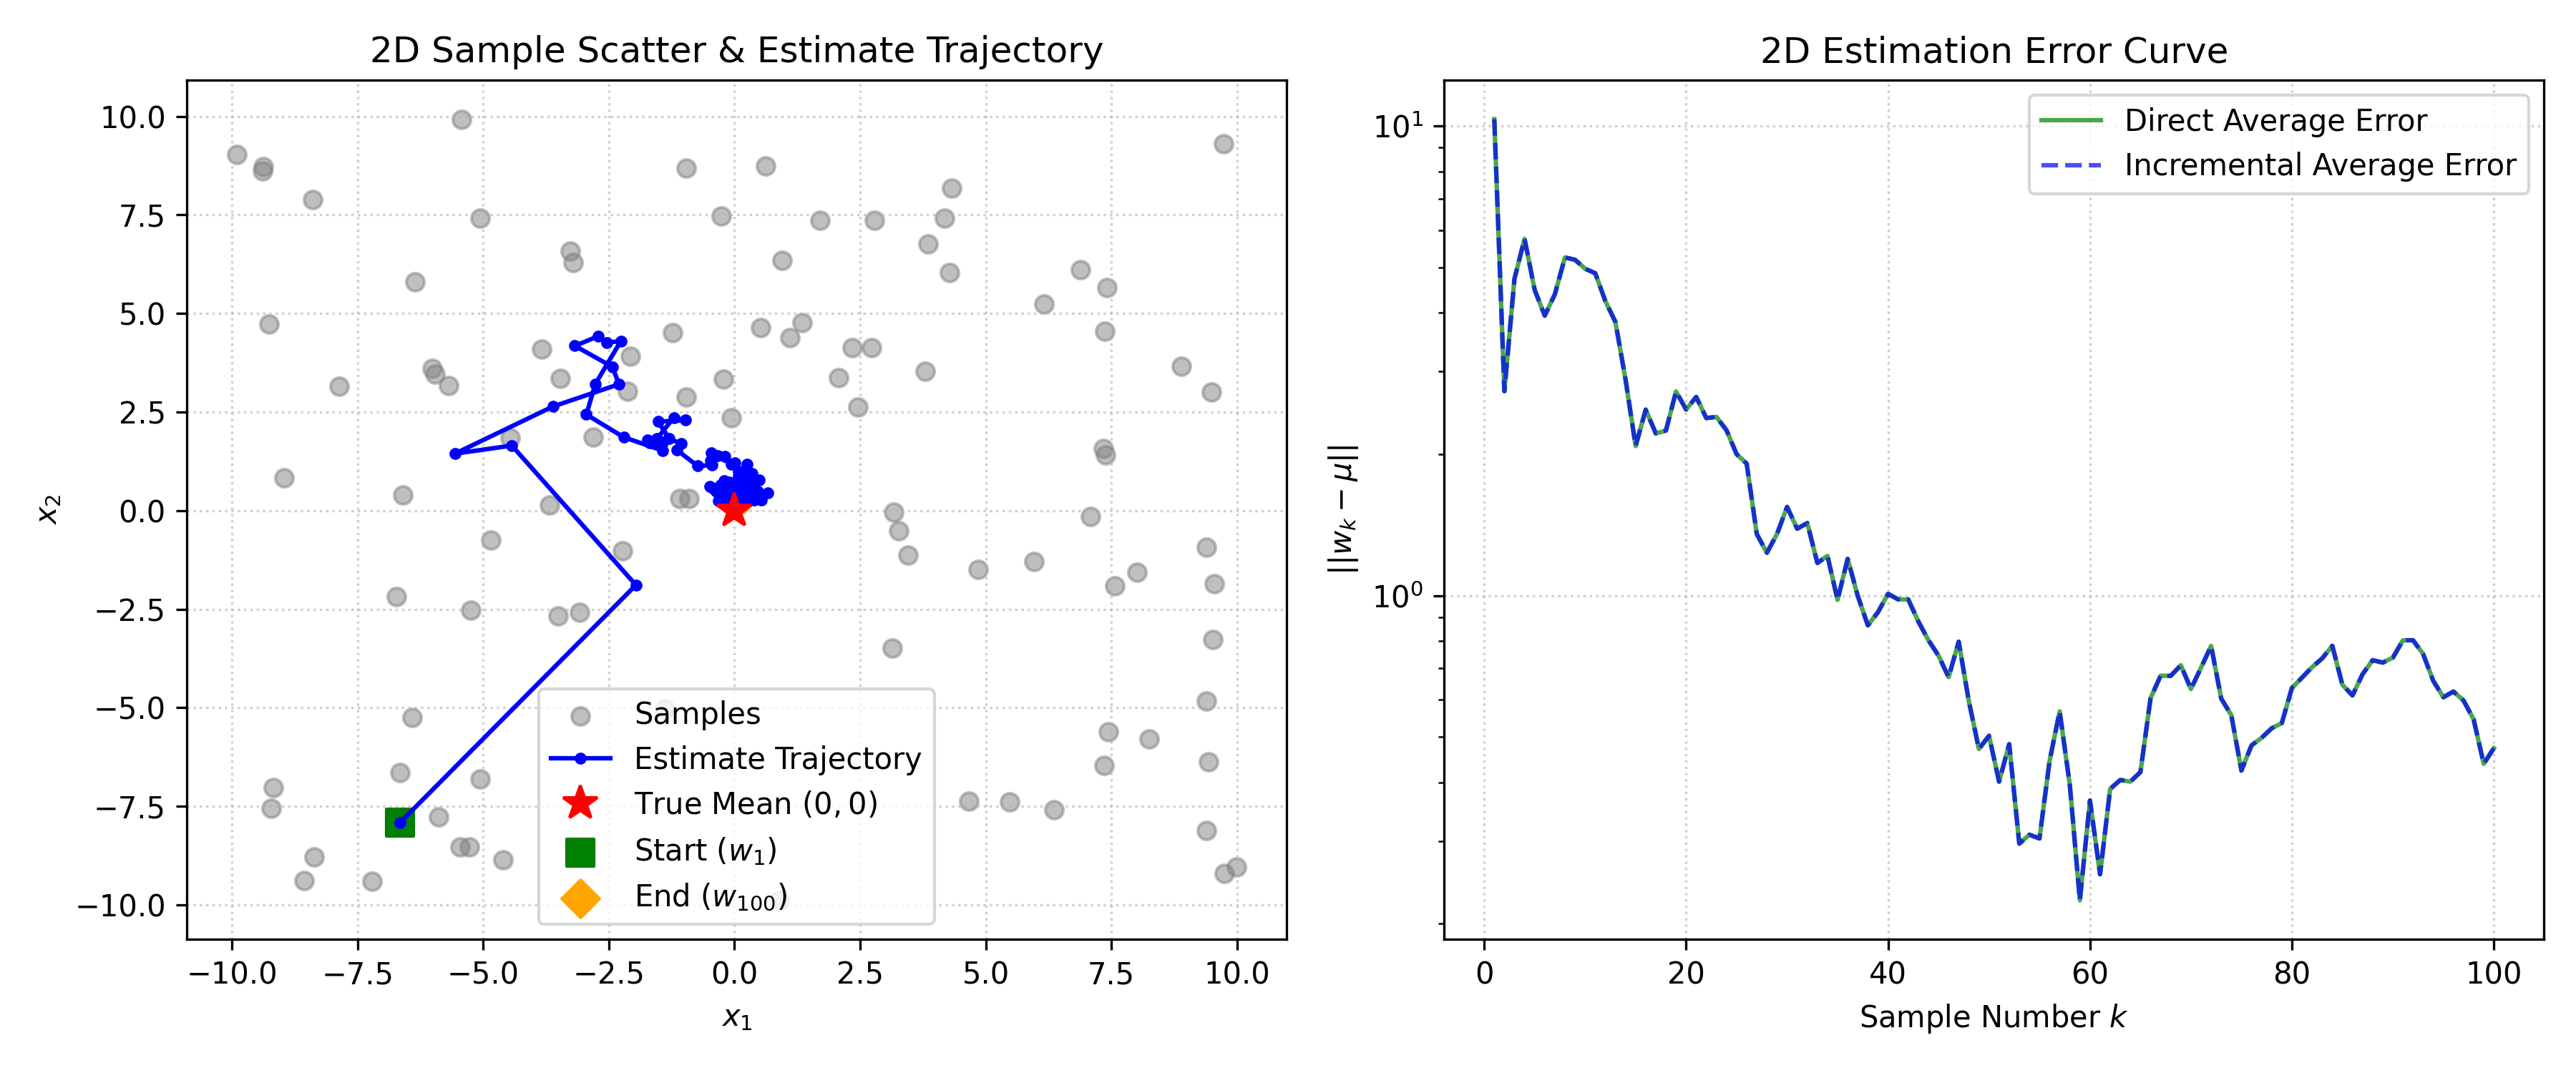
\includegraphics[width=0.75\textwidth]{exp3/results/task1_2d_sample_mean.png}
\caption{2D样本散点与估计轨迹及误差曲线}
\end{figure}

\paragraph{思考题}



\textbf{问题 1：为什么样本数量 $N$ 增大时，样本均值会逐渐接近真实期望？}


\answerlabel 这由\textbf{大数定律（Law of Large Numbers, LLN）}决定。
根据辛钦大数定律（Khinchin's Weak Law of Large Numbers），若随机变量序列 $X_1, X_2, \dots, X_N$ 独立同分布（i.i.d.），且具有有限的数学期望 $\mathbb{E}[X] = \mu$，则对于任意给定的正数 $\epsilon > 0$，有：
$$\lim_{N \to \infty} P\left( \left| \frac{1}{N}\sum_{i=1}^N X_i - \mu \right| < \epsilon \right) = 1$$
即样本均值依概率收敛于真实期望 $\mu$。
此外，根据中心极限定理（Central Limit Theorem, CLT），当样本量 $N$ 较大时，样本均值的分布近似为正态分布：
$$\bar{X}_N \sim N\left(\mu, \frac{\sigma^2}{N}\right)$$
其估计误差的方差为 $\frac{\sigma^2}{N}$。随着样本量 $N \to \infty$，估计的方差收敛于 0，因此样本均值在均方意义下也收敛于真实期望 $\mu$，逐渐接近真实期望。


\textbf{问题 2：增量形式相比一次性求和有什么实现优势？}


\answerlabel 增量形式的主要实现优势体现在\textbf{空间复杂度}和\textbf{计算流式化（实时在线处理）}：
\begin{itemize}
\item \textbf{空间复杂度低}：一次性求和需要首先将全部 $N$ 个样本存储在内存中，空间复杂度为 $O(N)$。若数据规模极大（如数亿级样本），会导致内存溢出。而增量形式只需维护当前的估计值 $w_{k-1}$ 和样本计数 $k$，无需保存历史样本，空间复杂度仅为 $O(1)$。
\item \textbf{支持流式/在线更新（Online Learning）}：在实际应用（如强化学习或实时传感器数据流）中，样本是随着时间一步一步到达的。一次性求和必须等所有数据收集完毕后才能计算；而增量更新可以在新样本到达时立即使其参与参数更新，提供实时的期望值估计。
\end{itemize}


\textbf{问题 3：增量均值为什么可以在不保存全部历史样本的情况下得到与普通样本均值一致的结果？（数学证明）}


\answerlabel

通过数学归纳法可以证明增量公式与直接平均的等价性。
设样本序列为 $x_1, x_2, \dots, x_k$。直接平均公式为：
$$\mu_k = \frac{1}{k} \sum_{i=1}^k x_i$$
增量平均递推公式为：
$$w_k = w_{k-1} - \frac{1}{k}(w_{k-1} - x_k), \quad w_0 = 0$$

\textbf{证明}：
\begin{enumerate}
\item \textbf{基础步}：当 $k = 1$ 时，
   $$w_1 = w_0 - \frac{1}{1}(w_0 - x_1) = 0 - (0 - x_1) = x_1$$
   直接平均值为：
   $$\mu_1 = \frac{1}{1} \sum_{i=1}^1 x_i = x_1$$
   因此，$w_1 = \mu_1$ 成立。
\end{enumerate}

\begin{enumerate}
\item \textbf{归纳步}：假设当 $k = m$ 时，增量平均值与直接平均值相等，即 $w_m = \mu_m = \frac{1}{m} \sum_{i=1}^m x_i$。
   那么当 $k = m + 1$ 时，根据递推公式：
   \[
   \begin{aligned}
   w_{m+1}
   &=w_m-\frac{1}{m+1}(w_m-x_{m+1})\\
   &=\frac{m}{m+1}w_m+\frac{1}{m+1}x_{m+1}.
   \end{aligned}
   \]
   代入归纳假设 $w_m = \frac{1}{m} \sum_{i=1}^m x_i$，有：
   \[
   \begin{aligned}
   w_{m+1}
   &=\frac{m}{m+1}\left(\frac{1}{m}\sum_{i=1}^{m}x_i\right)
     +\frac{1}{m+1}x_{m+1}\\
   &=\frac{1}{m+1}\sum_{i=1}^{m+1}x_i
    =\mu_{m+1}.
   \end{aligned}
   \]
\end{enumerate}

综上，根据数学归纳法，对任意 $k \ge 1$，均有 $w_k = \mu_k$ 成立。因此，增量公式不需要保留历史数据便可获得与直接求和完全一致的精确结果。

\subsubsection{任务 2：Robbins-Monro 随机近似与步长比较}

Robbins-Monro（RM）随机近似通过含噪迭代 $w_{k+1} = w_k - \alpha_k \tilde{g}(w_k, x_k)$ 求解方程 $g(w)=0$。算法收敛的充要条件是步长满足 RM 条件：$\sum \alpha_k = \infty$（保证纠偏能力）且 $\sum \alpha_k^2 < \infty$（保证方差被阻尼），在均值估计中即 $\tilde{g}(w_k, x_k) = w_k - x_k$。

一维实验最终绝对误差数据统计如下（基于 1000 次迭代）：

\begin{table}[H]
\centering
\begin{tabular}{ccccc}
\toprule
初始值 $w_0$ & $\alpha_k = 1/k$ & $\alpha_k = 1/k^{0.6}$ & $\alpha_k = 0.05$ (常数) & $\alpha_k = 1/k^2$ (过快) \\
\midrule
\textbf{-10.0} & 0.03061 & 0.06099 & 0.11345 & 0.06939 \\
\textbf{+10.0} & 0.03061 & 0.06099 & 0.11345 & 0.06939 \\
\bottomrule
\end{tabular}
\end{table}


\textbf{说明：}一维实验对两个初始值使用了相同的随机样本序列。表中各步长的最终误差相同，但两条轨迹在迭代前期仍存在明显差异；因此，最终误差不能单独反映初始值对收敛过程的影响。


1D 实验结果图：
\begin{figure}[H]
\centering
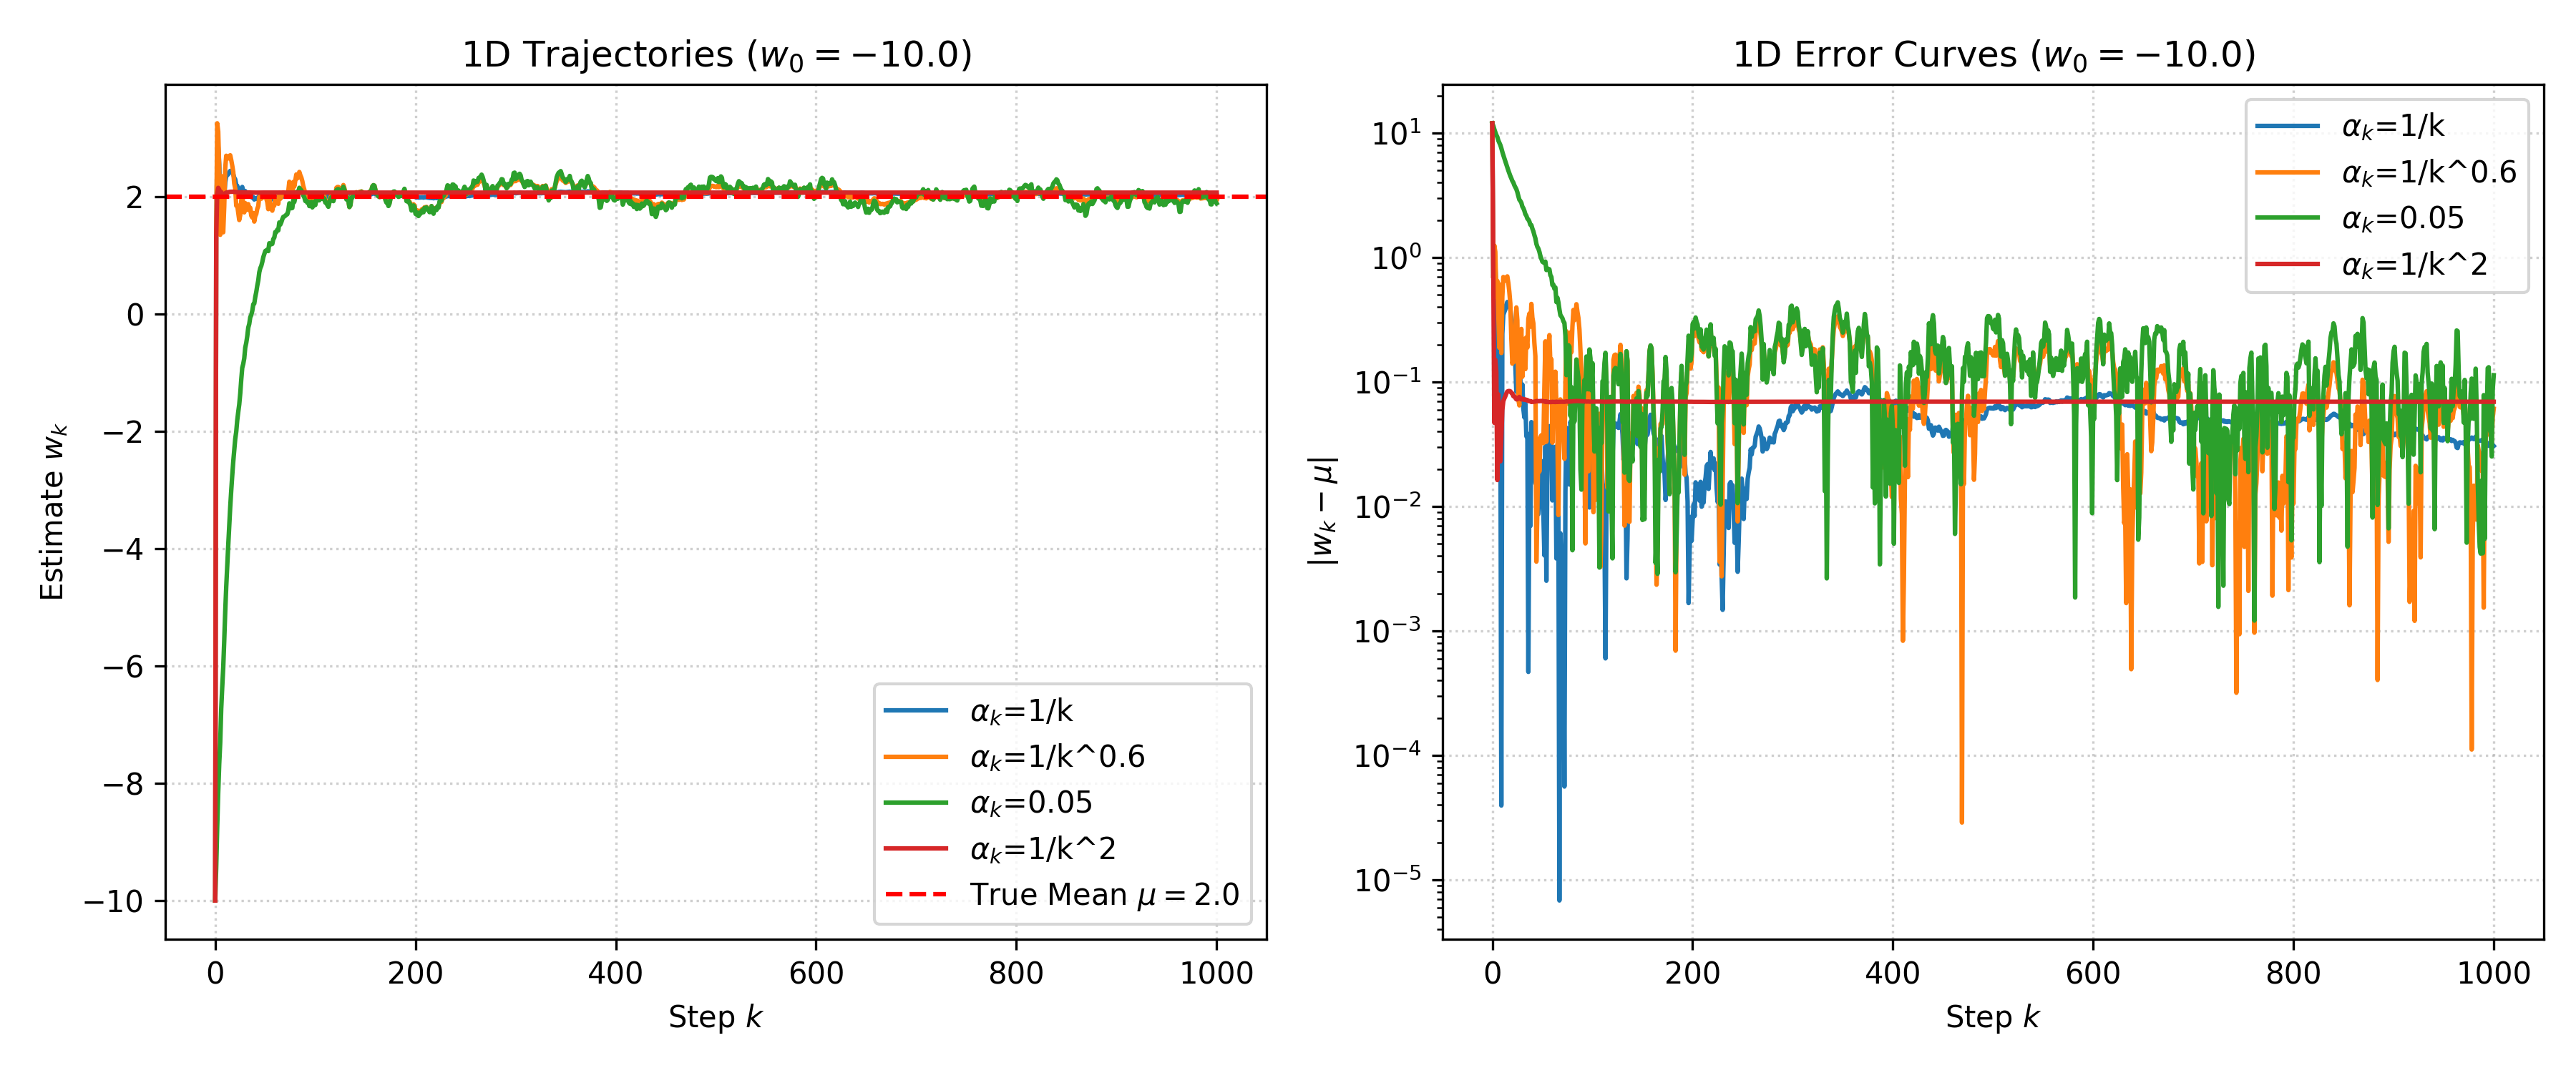
\includegraphics[width=0.75\textwidth]{exp3/results/task2_1d_w0_-10.png}
\caption{1D Robbins-Monro (初始值 w0 = -10.0) 收敛曲线}
\end{figure}
\begin{figure}[H]
\centering
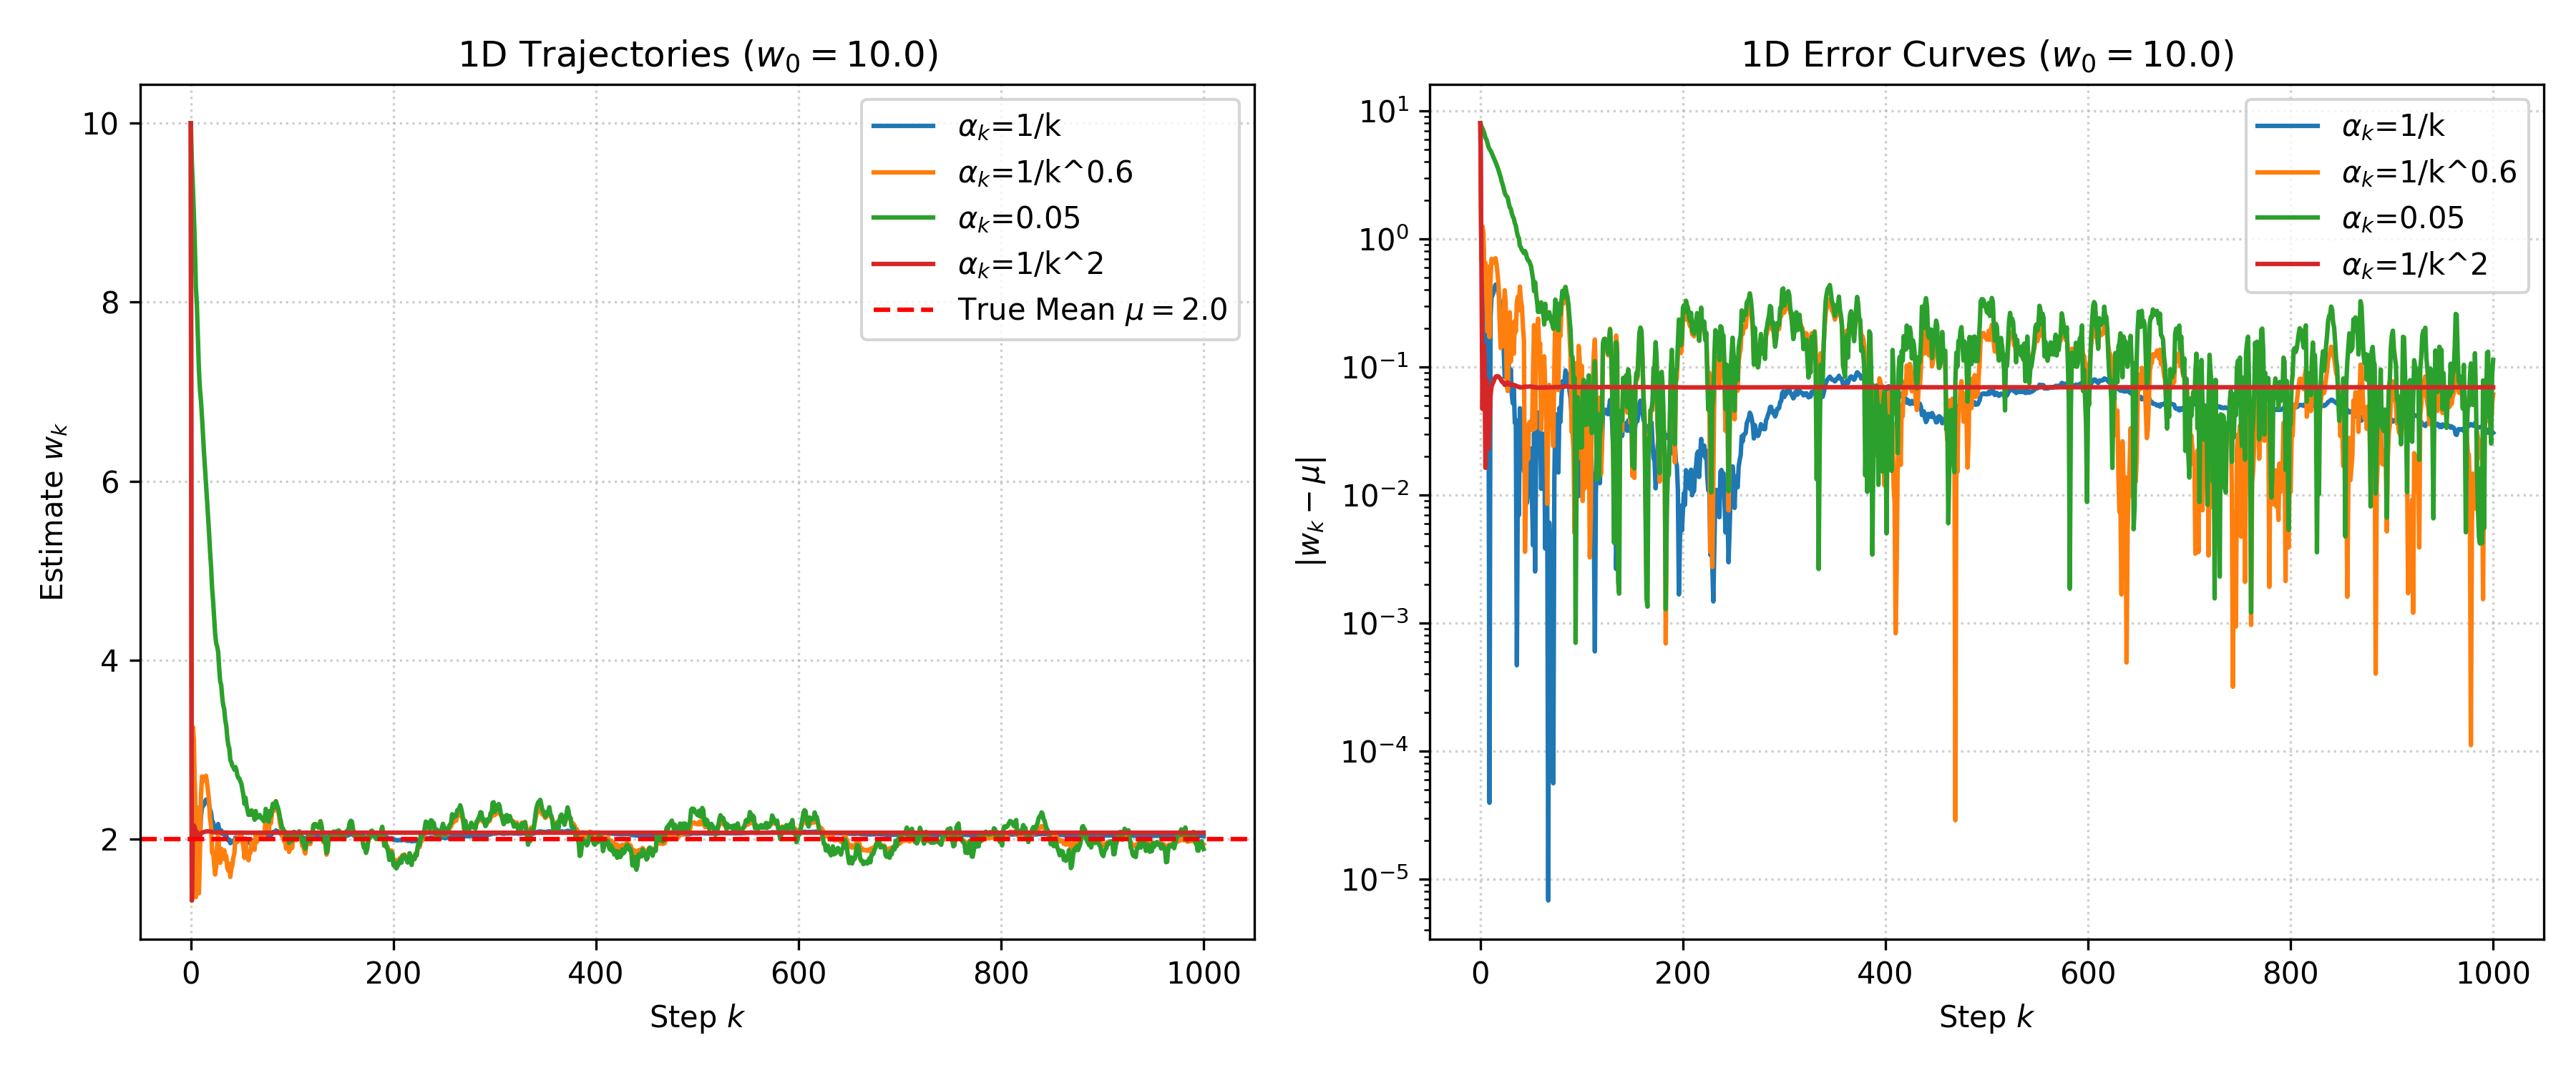
\includegraphics[width=0.75\textwidth]{exp3/results/task2_1d_w0_10.png}
\caption{1D Robbins-Monro (初始值 w0 = 10.0) 收敛曲线}
\end{figure}

2D 实验轨迹与误差曲线图：
\begin{figure}[H]
\centering
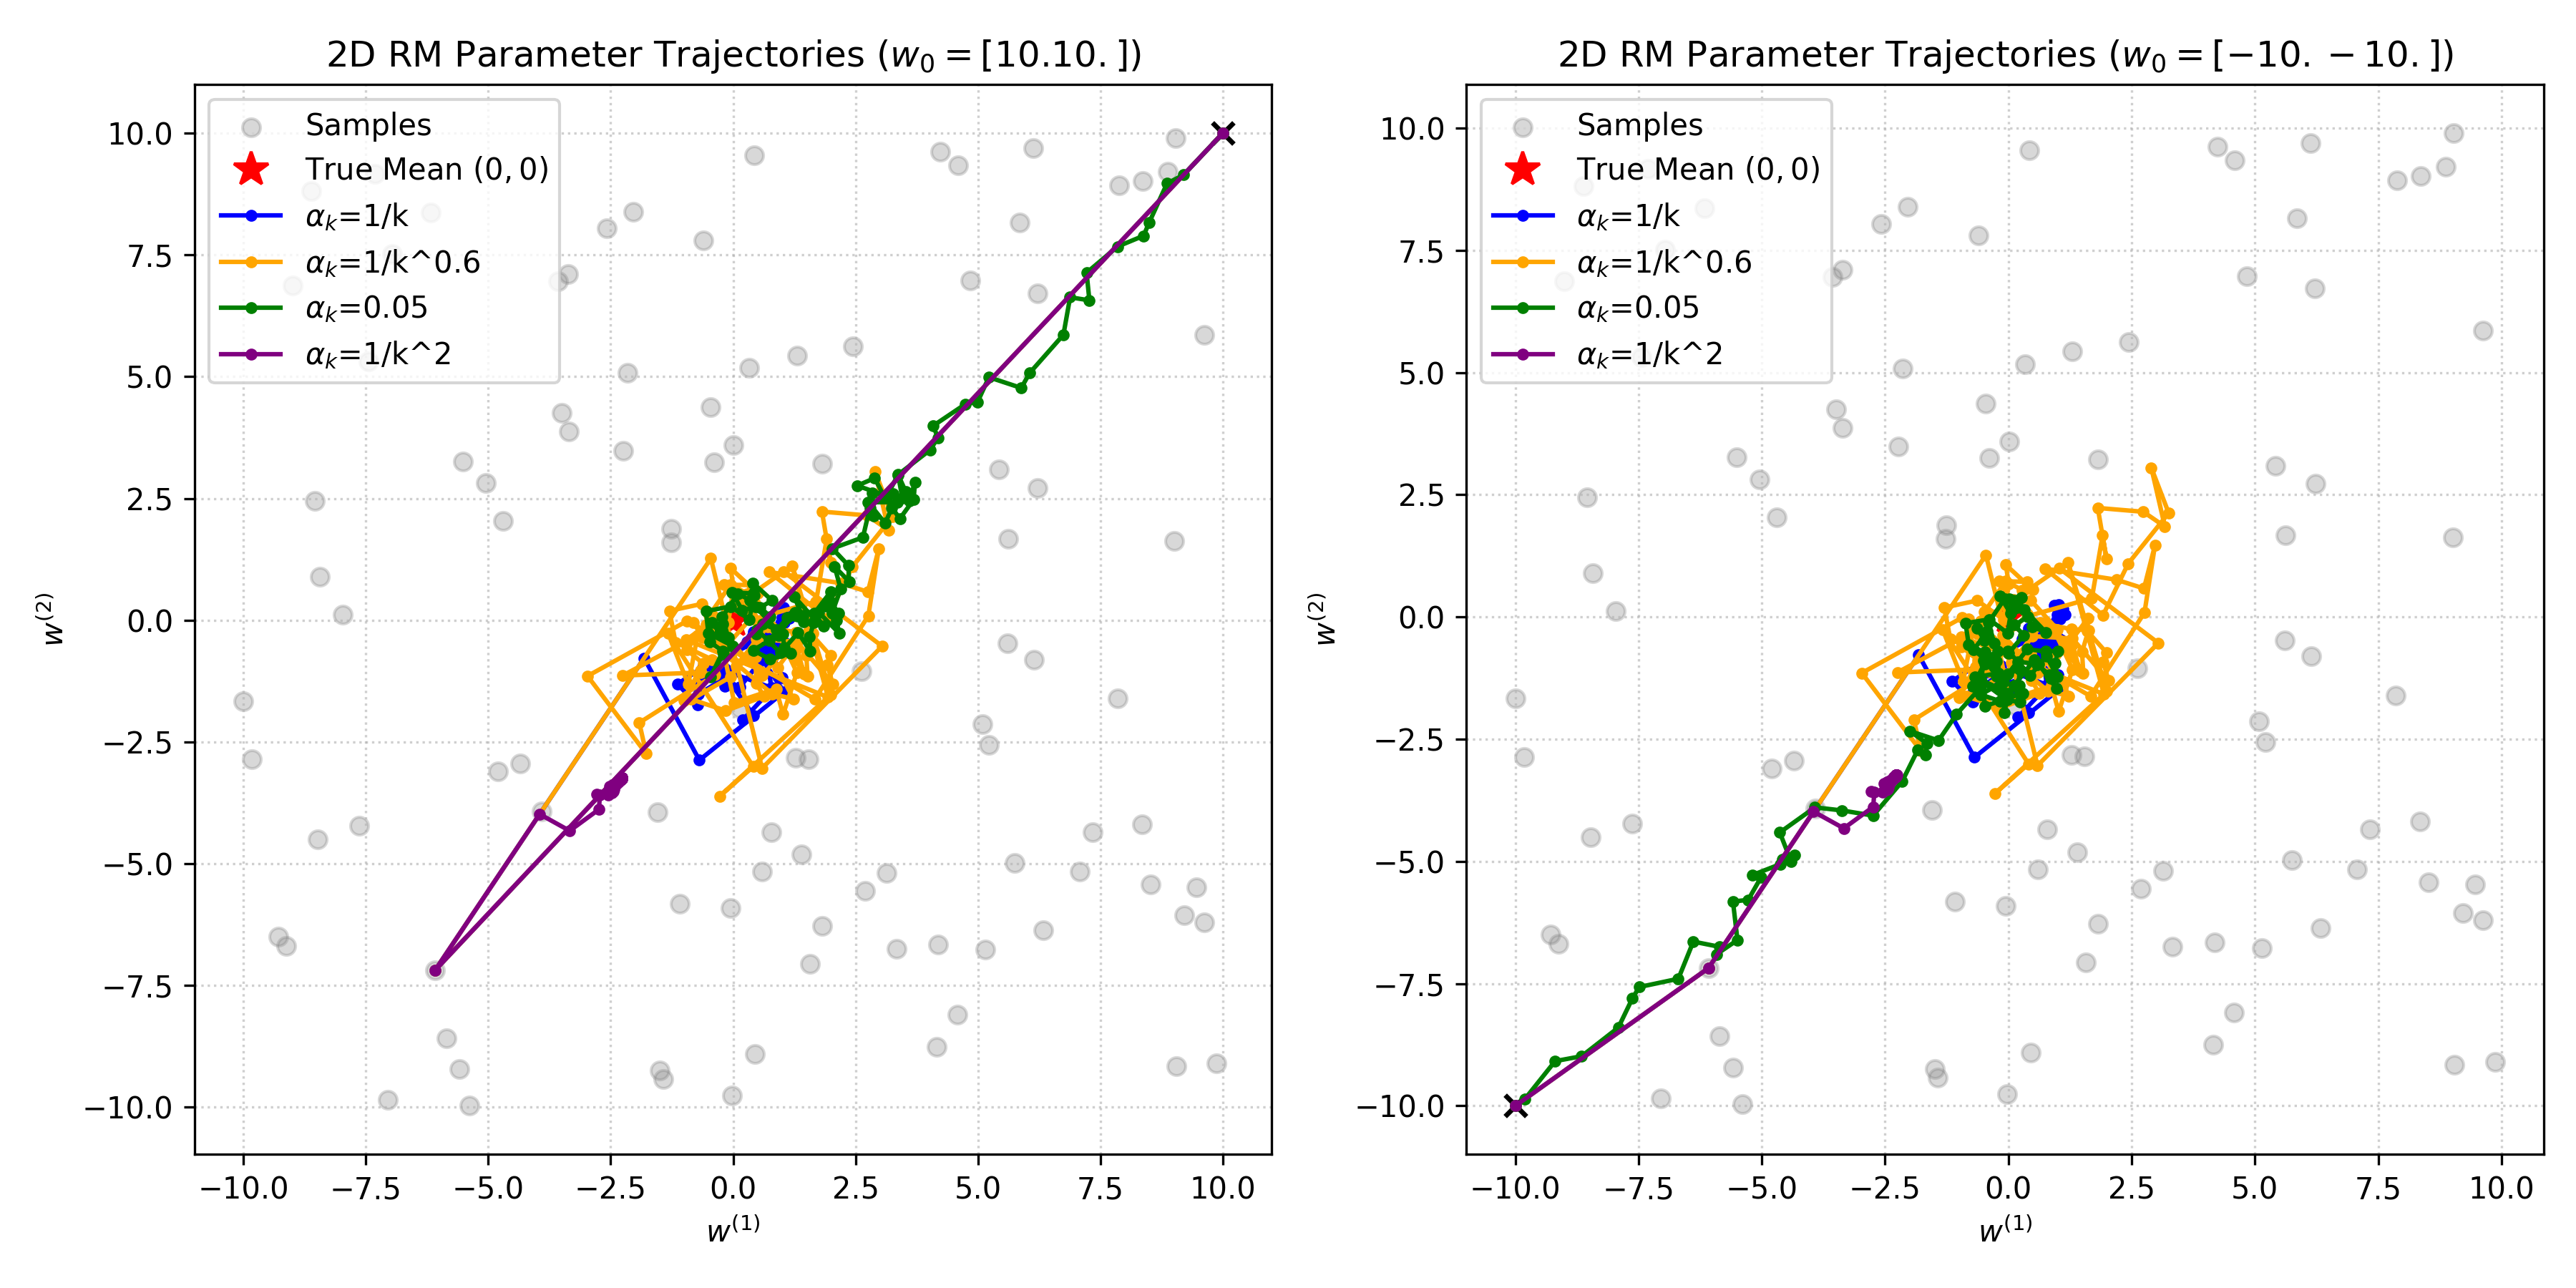
\includegraphics[width=0.75\textwidth]{exp3/results/task2_2d_trajectories.png}
\caption{2D Robbins-Monro 估计轨迹比较}
\end{figure}
\begin{figure}[H]
\centering
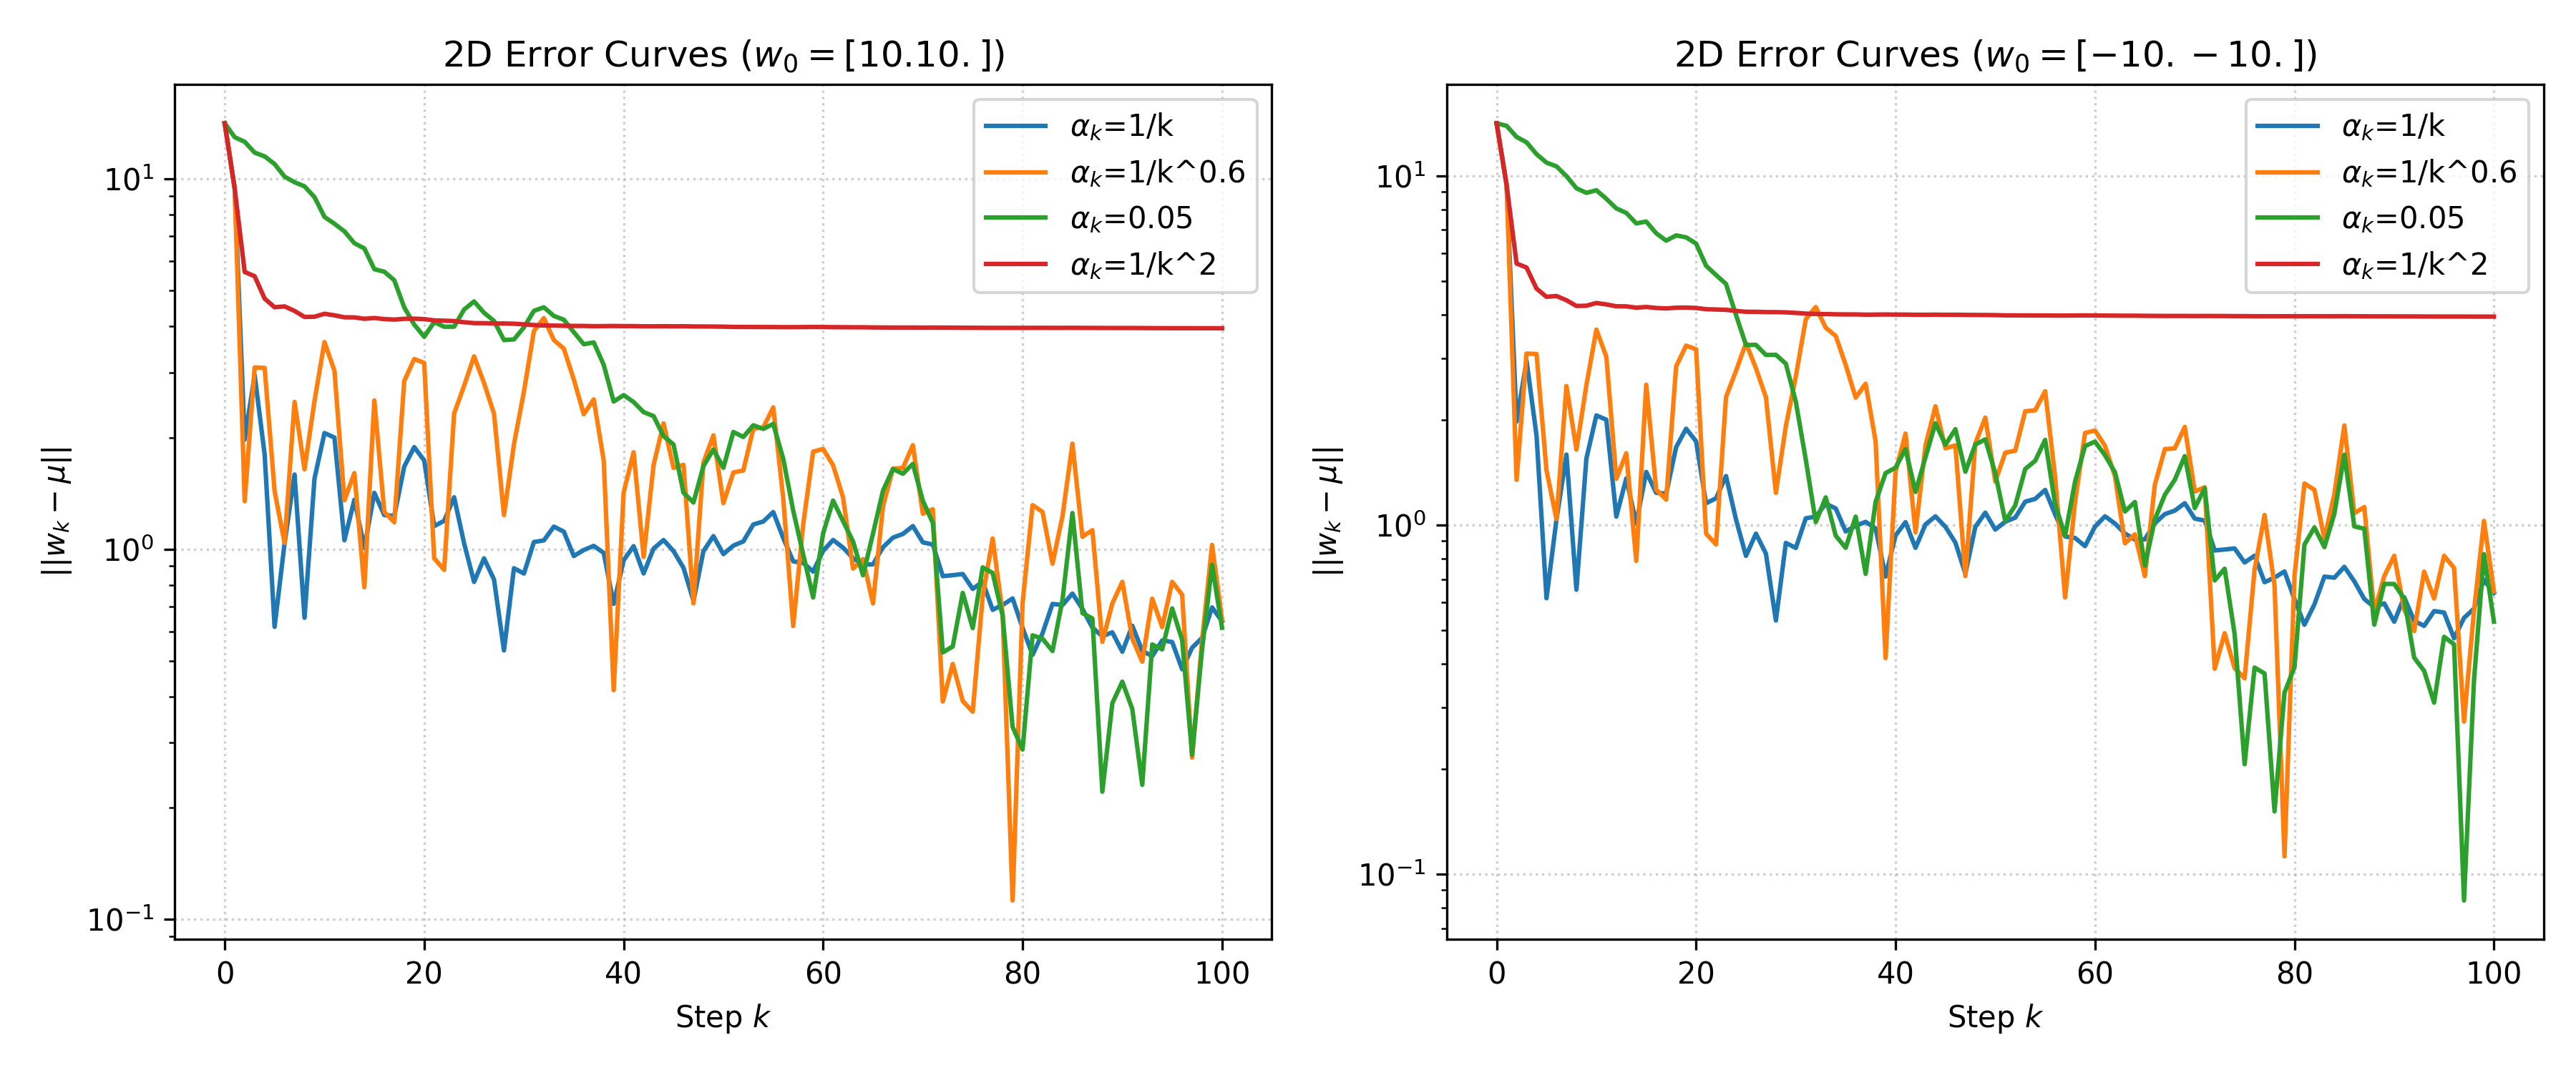
\includegraphics[width=0.75\textwidth]{exp3/results/task2_2d_errors.png}
\caption{2D Robbins-Monro 误差曲线比较}
\end{figure}

\paragraph{思考题}


问题 1：Robbins-Monro 方法中的噪声项需要满足什么性质？若样本噪声存在系统性偏差，会对估计结果产生什么影响？


\answerlabel 
在迭代 $w_{k+1}=w_k-\alpha_k(g(w_k)+\eta_k)$ 中，噪声通常需要满足以下条件：
\begin{enumerate}
\item \textbf{条件无偏性}：给定历史信息 $\mathcal{F}_k$ 后，当前噪声的条件期望为零，
     $$\mathbb{E}[\eta_k \mid \mathcal{F}_k] = 0$$
这意味着含噪观测在期望上仍指向原方程的根。
\item \textbf{条件二阶矩有界}：噪声幅度不能无限增长，通常要求
     $$\mathbb{E}[\|\eta_k\|^2 \mid \mathcal{F}_k] \le \sigma^2 < \infty$$
\end{enumerate}

若噪声存在系统性偏差 $b\neq0$，则算法实际求解的是 $g(w)+b=0$。在均值估计中，这会使估计值偏离真实均值，且该偏差不会通过增加迭代次数自动消失。


问题 2：为什么 $\alpha_k=1/k$ 通常能收敛，而常数步长可能在真值附近持续波动？请结合两个 Robbins--Monro 步长条件解释。


\answerlabel Robbins--Monro 步长需要同时满足
\[
\sum_{k=1}^{\infty}\alpha_k=\infty,\qquad
\sum_{k=1}^{\infty}\alpha_k^2<\infty.
\]
前一条件保证长期累计更新量足以修正初始误差，后一条件保证随机噪声的累计方差有限。

\begin{table}[H]
\centering
\begin{tabular}{cccc}
\toprule
步长设置 & $\sum\alpha_k=\infty$ & $\sum\alpha_k^2<\infty$ & 典型表现 \\
\midrule
$\alpha_k=1/k$ & 满足 & 满足 & 收敛到真实解 \\
$\alpha_k=\alpha$ & 满足 & 不满足 & 在真实解邻域持续波动 \\
$\alpha_k=1/k^2$ & 不满足 & 满足 & 可能在到达真实解前停滞 \\
\bottomrule
\end{tabular}
\end{table}

\paragraph{$\alpha_k=1/k$}
调和级数发散，说明算法始终保留足够的累计纠偏能力；平方和收敛，则使后期噪声影响逐步减弱。因此该步长兼顾了到达真实解和抑制随机波动两个要求。

\paragraph{常数步长 $\alpha_k=\alpha$}
常数步长的平方和发散。参数到达真实解附近后，新的随机样本仍会产生固定量级的更新，因此轨迹不会稳定在单一点上，而会在真实解邻域持续波动。

\paragraph{过快衰减步长 $\alpha_k=1/k^2$}
该步长的总和有限。如果初始值距离真实解较远，后期剩余的累计更新量可能不足以消除初始偏差，从而停在错误位置附近。

\conclusionlabel 两个条件分别约束“是否还有足够能力继续纠偏”和“噪声影响能否被逐步削弱”。实验中的收敛、波动与提前停滞正对应这三种条件组合。

\subsubsection{任务 3：BGD、MBGD与SGD的随机优化对比}

三种梯度下降方法在单步计算代价与梯度估计精度之间各有权衡：BGD 使用全部 $N$ 个样本的精确梯度，方差为零但每步代价 $O(Nd)$；SGD 每步随机抽取一个样本，代价 $O(d)$ 但梯度方差极大；MBGD 以 batch size $m$ 为中间权衡，梯度方差约为单样本方差的 $1/m$。

\paragraph{结果数据}
按照第 3.2.4 节的对比设计，各算法从 $w_0=[15,15]^\top$ 出发训练 30 个 epochs。下表给出单次运行相对于 $w^*=[0,0]^\top$ 的最终误差：

\begin{table}[H]
\centering
\begin{tabular}{ccccc}
\toprule
学习率设置 & BGD ($m=100$) & MBGD ($m=50$) & MBGD ($m=5$) & SGD ($m=1$) \\
\midrule
\textbf{固定 $\alpha=0.1$} & 0.47291 & 0.41411 & 0.20428 & 0.97657 \\
\textbf{衰减 $\alpha_k$} & 2.69893 & 0.75396 & 0.43867 & 0.46005 \\
\bottomrule
\end{tabular}
\end{table}

BGD、MBGD、SGD 在 2D 空间中的优化轨迹以及误差收敛曲线：

\begin{figure}[H]
\centering
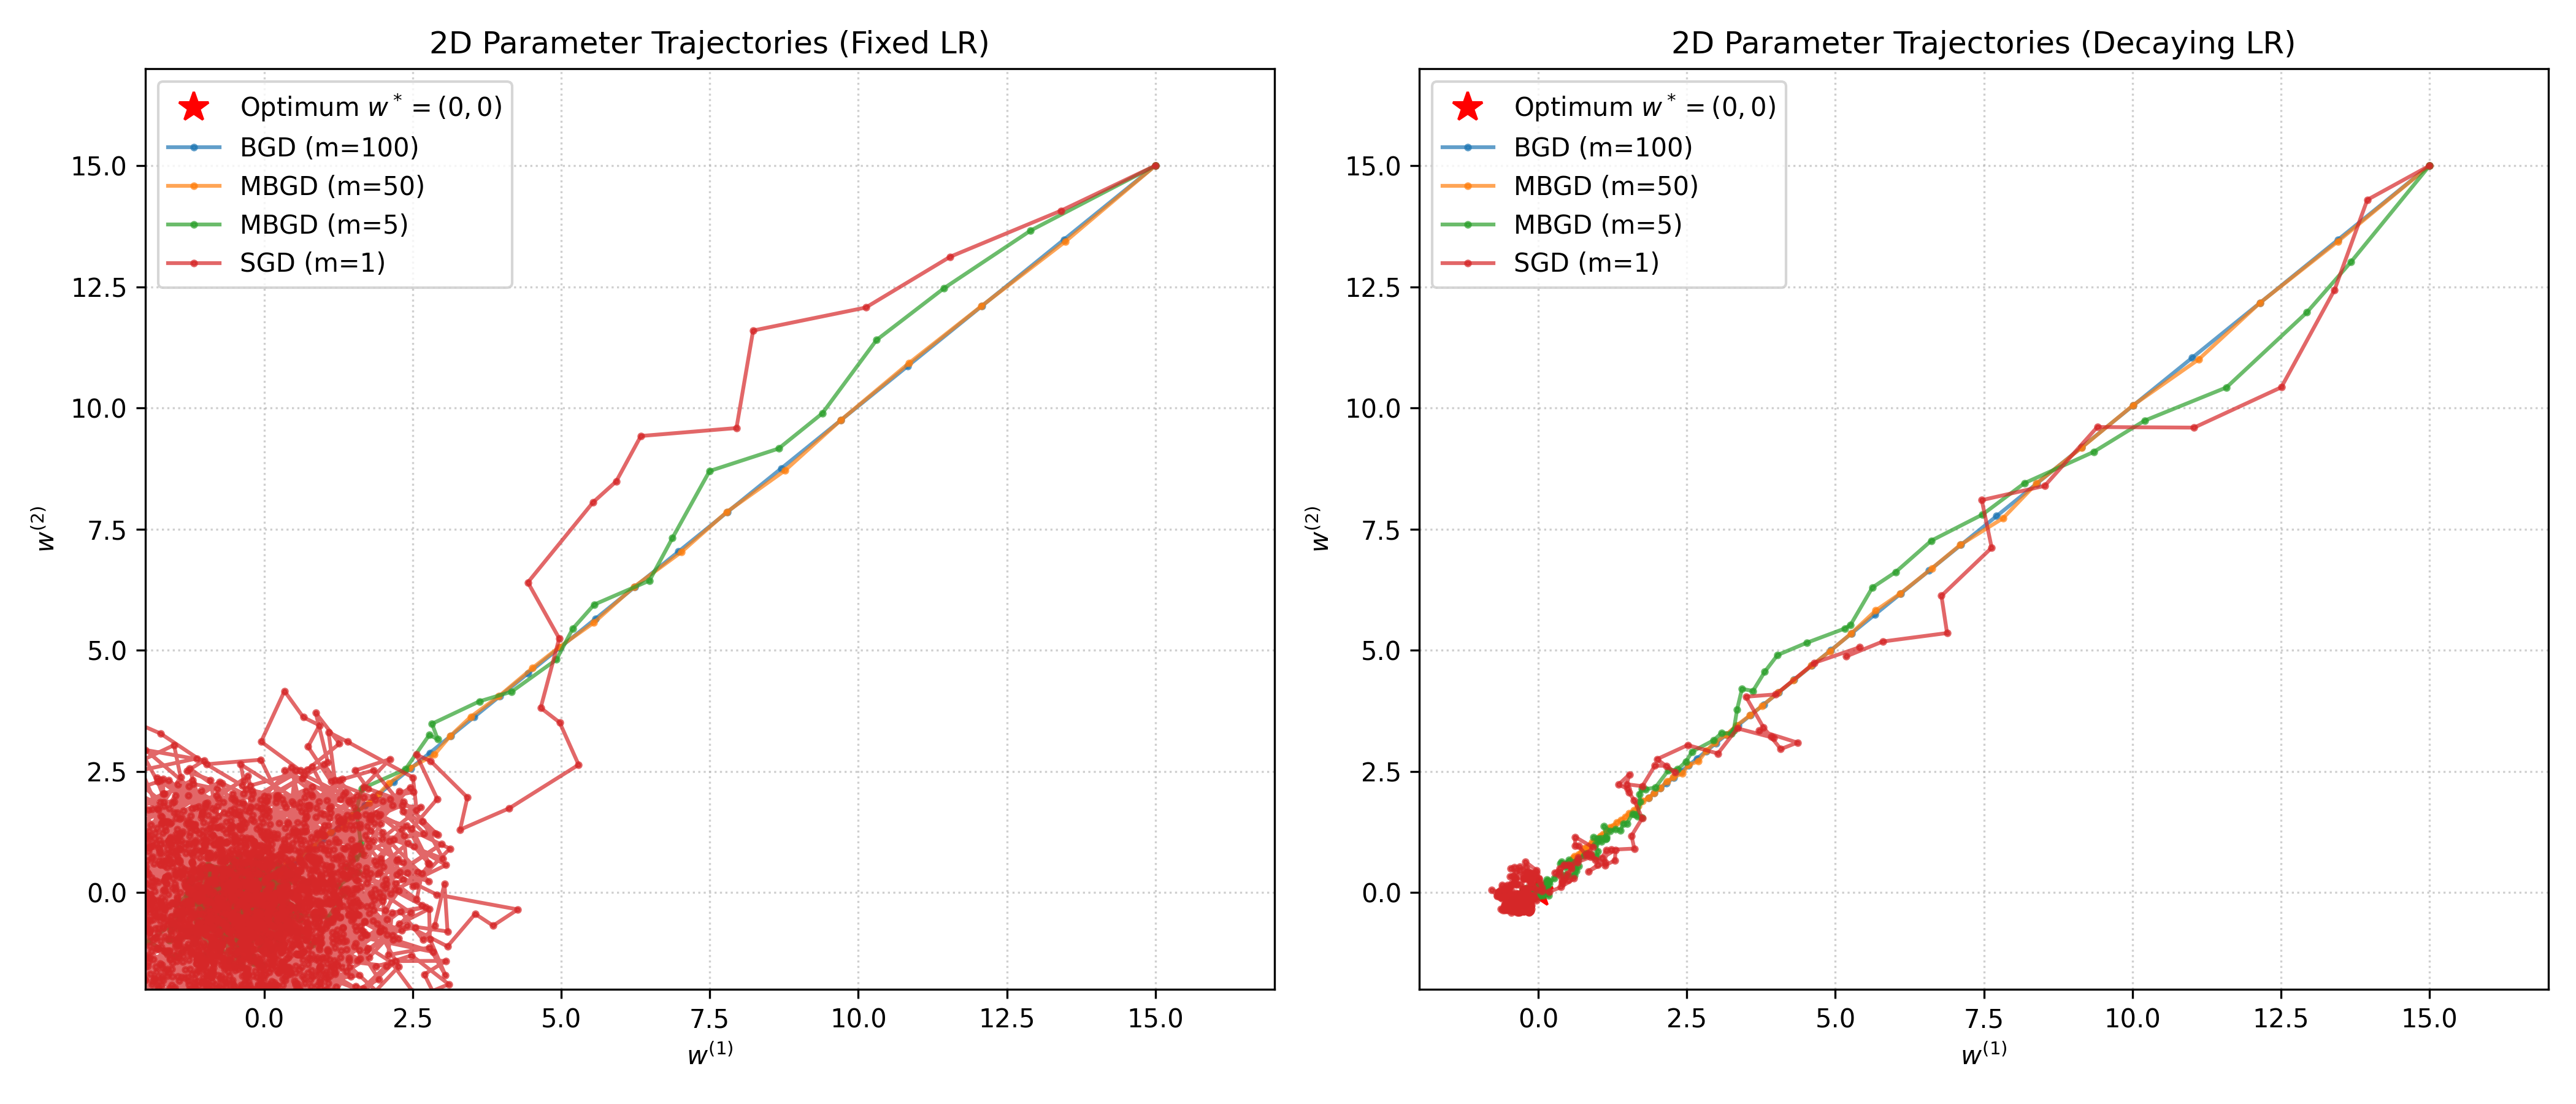
\includegraphics[width=0.75\textwidth]{exp3/results/task3_trajectories_2d.png}
\caption{BGD, MBGD, SGD 优化轨迹比较 (2D空间)}
\end{figure}
\begin{figure}[H]
\centering
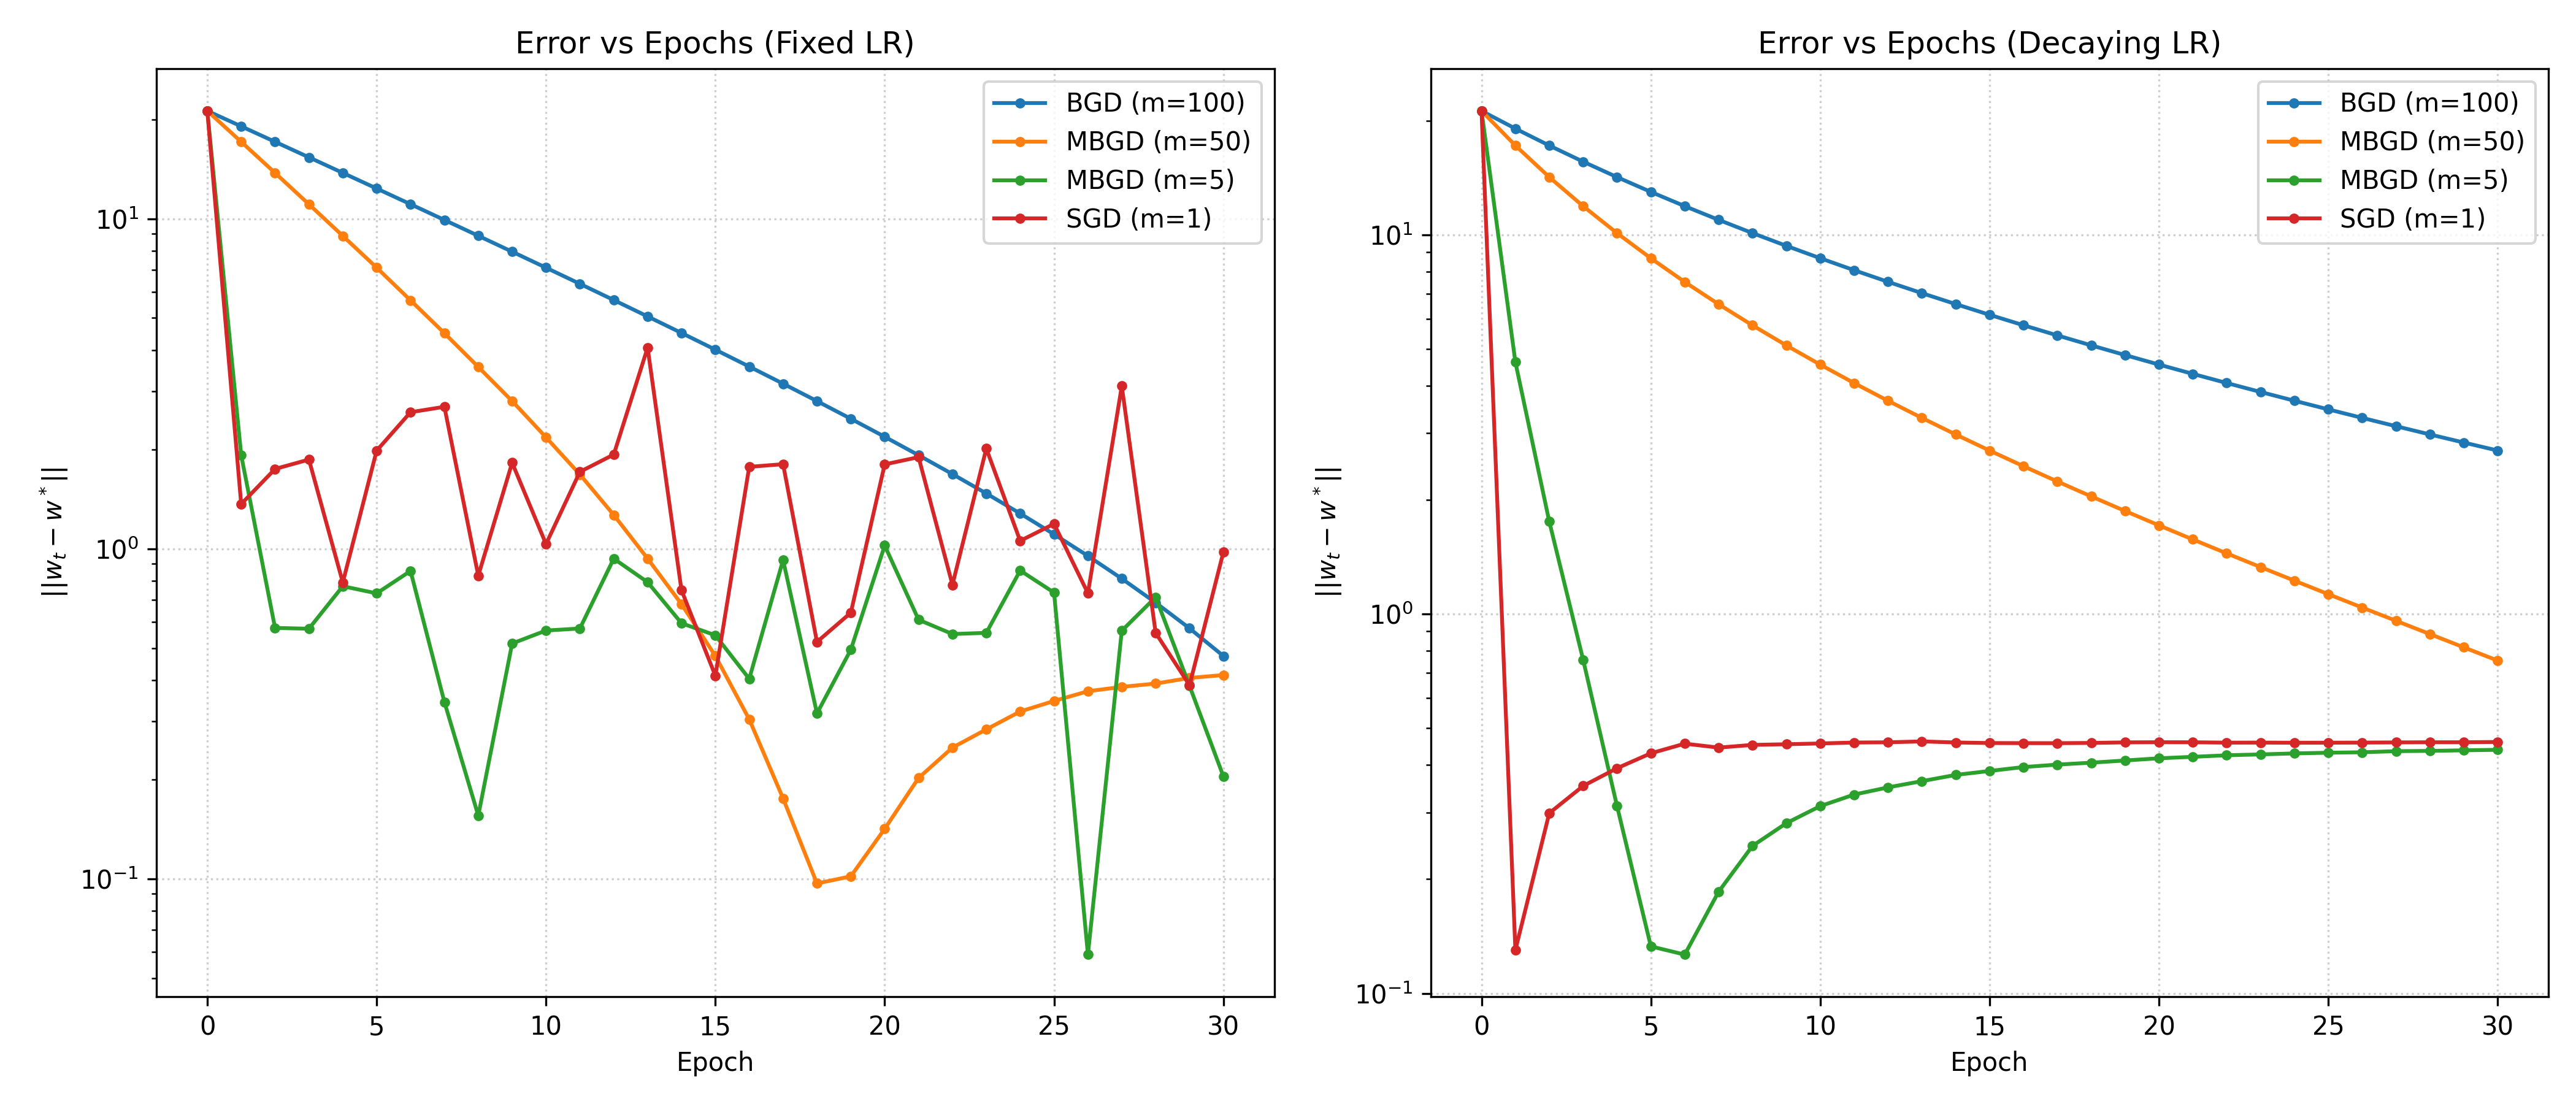
\includegraphics[width=0.75\textwidth]{exp3/results/task3_error_vs_epochs.png}
\caption{BGD, MBGD, SGD 误差随Epoch变化曲线}
\end{figure}
\begin{figure}[H]
\centering
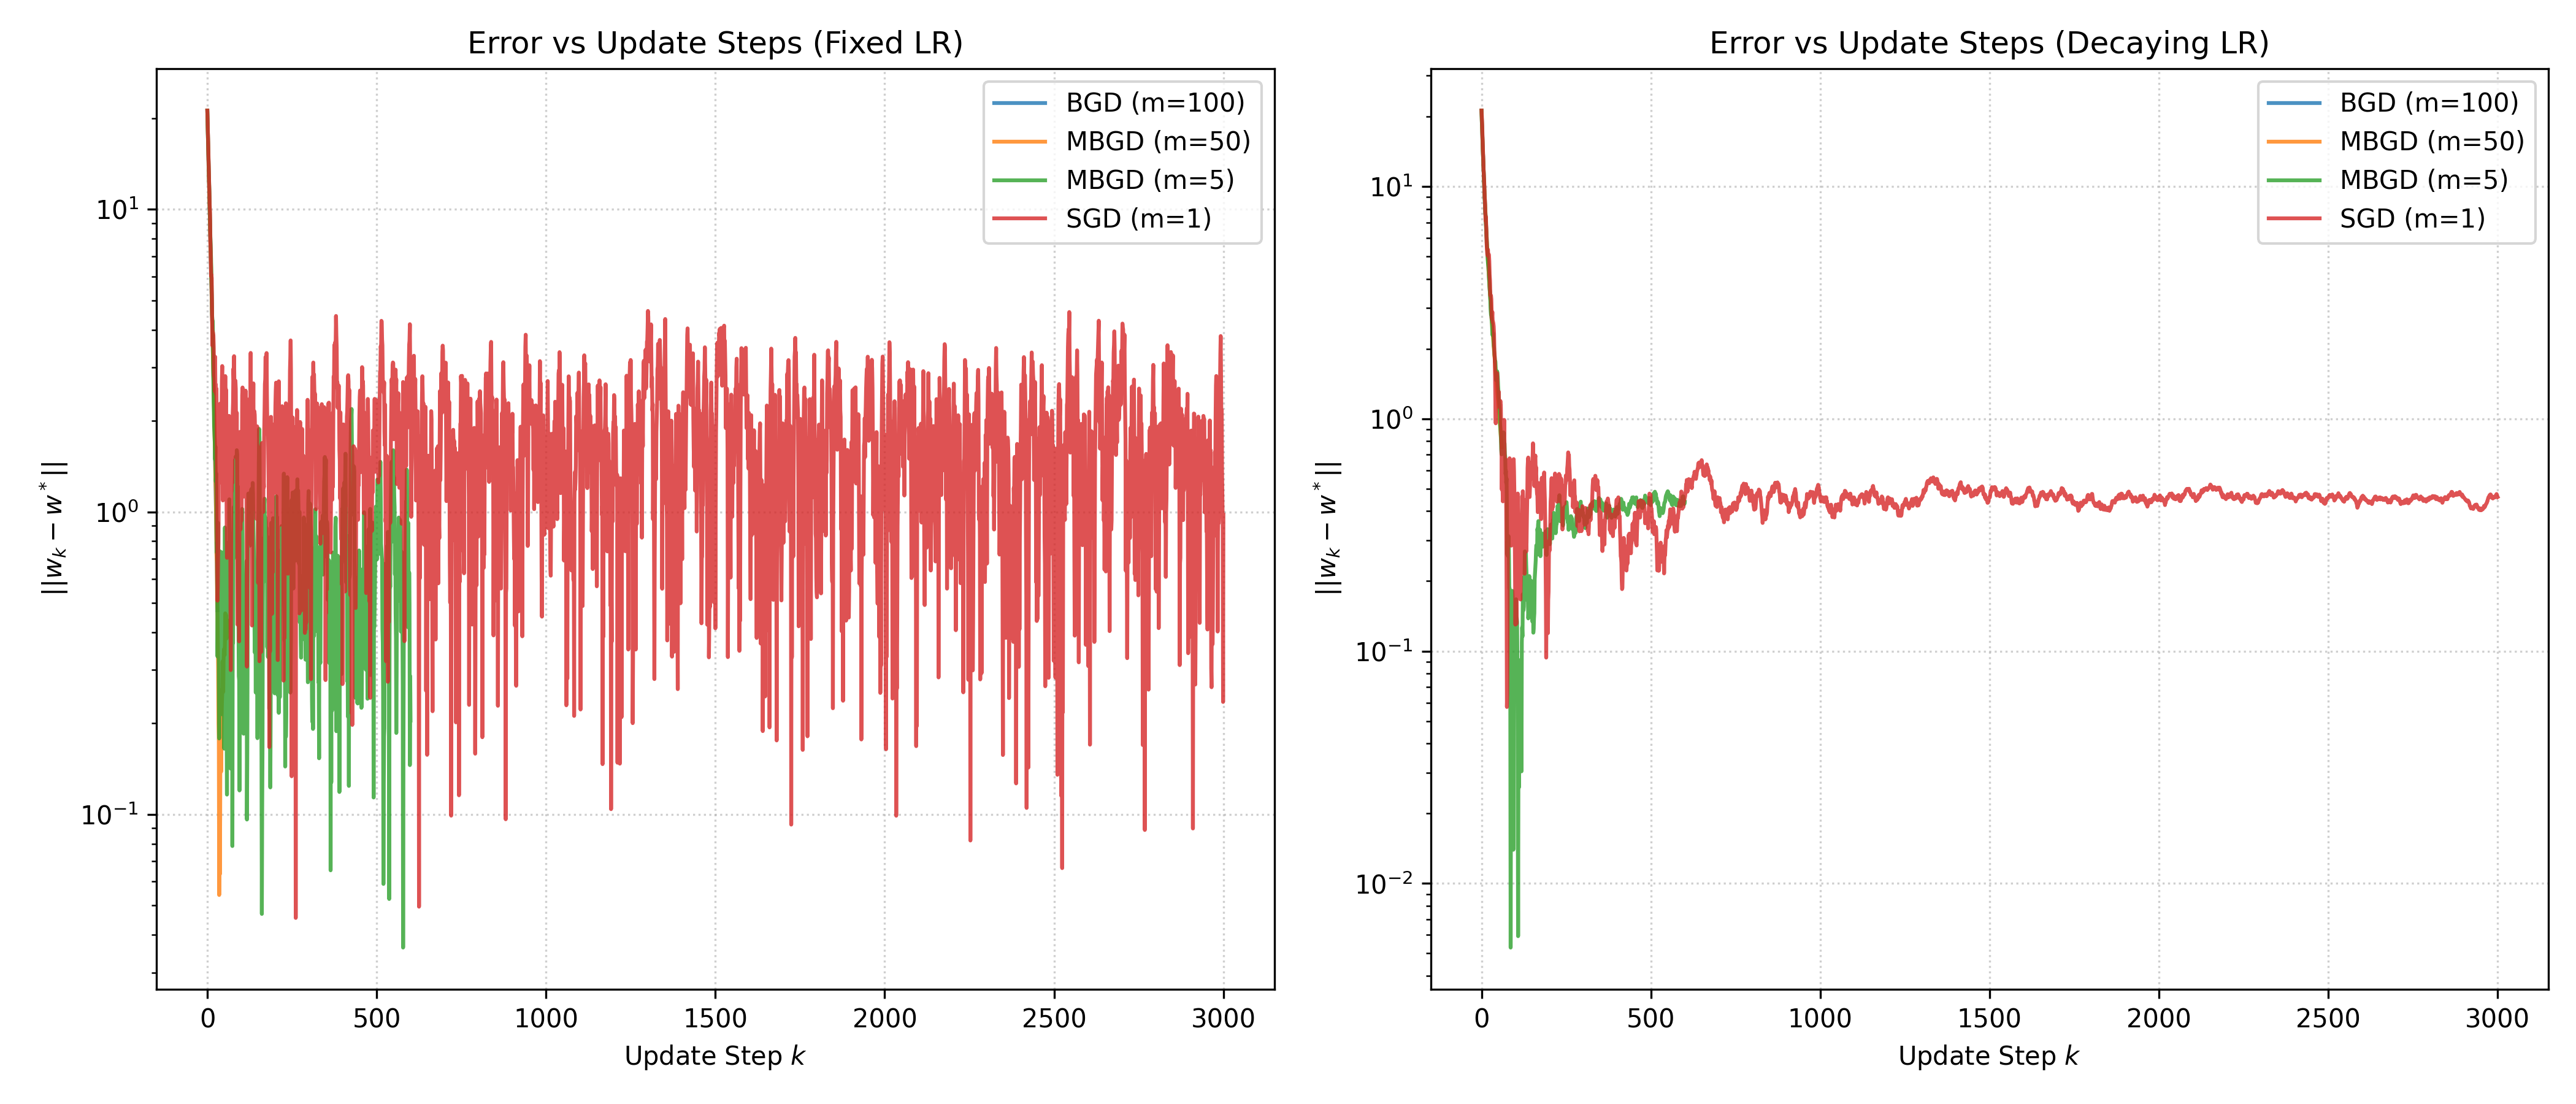
\includegraphics[width=0.75\textwidth]{exp3/results/task3_error_vs_steps.png}
\caption{BGD, MBGD, SGD 误差随Update Step变化曲线}
\end{figure}

\paragraph{思考题}



\textbf{问题 1：为什么 SGD 的曲线更抖动，但单步计算代价更低？}


\answerlabel 
\begin{itemize}
\item \textbf{曲线抖动原因}：SGD（随机梯度下降）在每次更新时，仅随机选择\textbf{一个}样本 $x_i$ 计算梯度并更新参数：$g_k = w - x_i$。该梯度是全局真实梯度的无偏估计，即 $\mathbb{E}[w - X] = \nabla J(w)$，但其单个样本的随机性使得其方差极其巨大。当该单个样本偏离均值较大时，更新方向可能会偏离最优下降方向甚至相反，导致参数轨迹频繁改变方向，呈现出剧烈的锯齿状抖动。
\item \textbf{单步计算代价低的原因}：BGD 需要对全部 $N$ 个样本求和计算平均梯度：
\[
\nabla J(w) = \frac{1}{N} \sum_{i=1}^N (w - x_i).
\]
在 $d$ 维空间下，其单步时间复杂度为 $O(Nd)$；SGD 每步只计算一个样本的梯度，复杂度为 $O(d)$。因此，在相同数据集下，SGD 的单步计算量约为 BGD 的 $1/N$（本实验中 $N=100$）。
\end{itemize}

问题 2：batch size 增大时，梯度估计方差和单步计算时间分别如何变化？
\answerlabel 
\begin{itemize}
\item \textbf{梯度估计方差的变化}：
  假设单个样本梯度的协方差矩阵为 $\Sigma$。对于 batch size 为 $m$ 的随机梯度估计：
  $$g_{MB} = \frac{1}{m}\sum_{j=1}^m \nabla_w f(w, X_{i_j})$$
  若样本是独立同分布采样的，则小批量梯度的协方差矩阵为：
  $$\text{Var}(g_{MB}) = \frac{1}{m} \Sigma$$
  即梯度估计方差与批量大小 $m$ \textbf{成反比}。随着 batch size $m$ 增大，方差以 $1/m$ 的速度衰减，梯度估计变得越来越平滑，逼近 BGD 的真实确定性梯度。
\item \textbf{单步计算时间的变化}：
  单步计算时间与批量大小 $m$ \textbf{呈线性增加关系}（单核串行计算下时间复杂度为 $O(md)$）。对于大规模计算平台，利用 GPU/CPU 的 SIMD 并行加速，在 $m$ 较小时（未达到硬件吞吐上限）单步时间增长较平缓，但总体趋势仍是随着 $m$ 增大，所需的算力与耗时线性/亚线性上升。
\end{itemize}

\subsubsection{任务 4：随机近似收敛现象分析（扩展）}

本任务通过多随机种子统计分析与异常样本敏感度实验，深入分析随机性对实验结论的影响及各优化算法的鲁棒性差异。多种子统计排除个体样本的偶发性偏差；异常样本实验则揭示 BGD（隐式系统偏差）与 SGD（显式瞬态抖动）面对有偏数据时的本质性行为差异。

\paragraph{1. 20 个随机种子统计分析}
在 20 个不同的随机种子下，重新生成样本并运行各算法，统计其最终误差 $\|w_{final} - w^*\|$ 的均值和标准差。结果如下：

\begin{table}[H]
\centering
\begin{tabular}{cccc}
\toprule
学习率类型 & 优化方法 & 误差均值 (Mean Error) & 误差标准差 (Std Error) \\
\midrule
\textbf{Fixed} & BGD (m=100) & 0.97971 & 0.27174 \\
\textbf{Fixed} & MBGD (m=50) & 0.57264 & 0.34862 \\
\textbf{Fixed} & MBGD (m=5) & 0.61620 & 0.35826 \\
\textbf{Fixed} & SGD (m=1) & 1.67644 & 0.90371 \\
\textbf{Decaying} & BGD (m=100) & 3.01916 & 0.34552 \\
\textbf{Decaying} & MBGD (m=50) & 1.20914 & 0.28016 \\
\textbf{Decaying} & MBGD (m=5) & 0.57724 & 0.35927 \\
\textbf{Decaying} & SGD (m=1) & 0.57894 & 0.36153 \\
\bottomrule
\end{tabular}
\end{table}

统计结果可视化：
\begin{figure}[H]
\centering
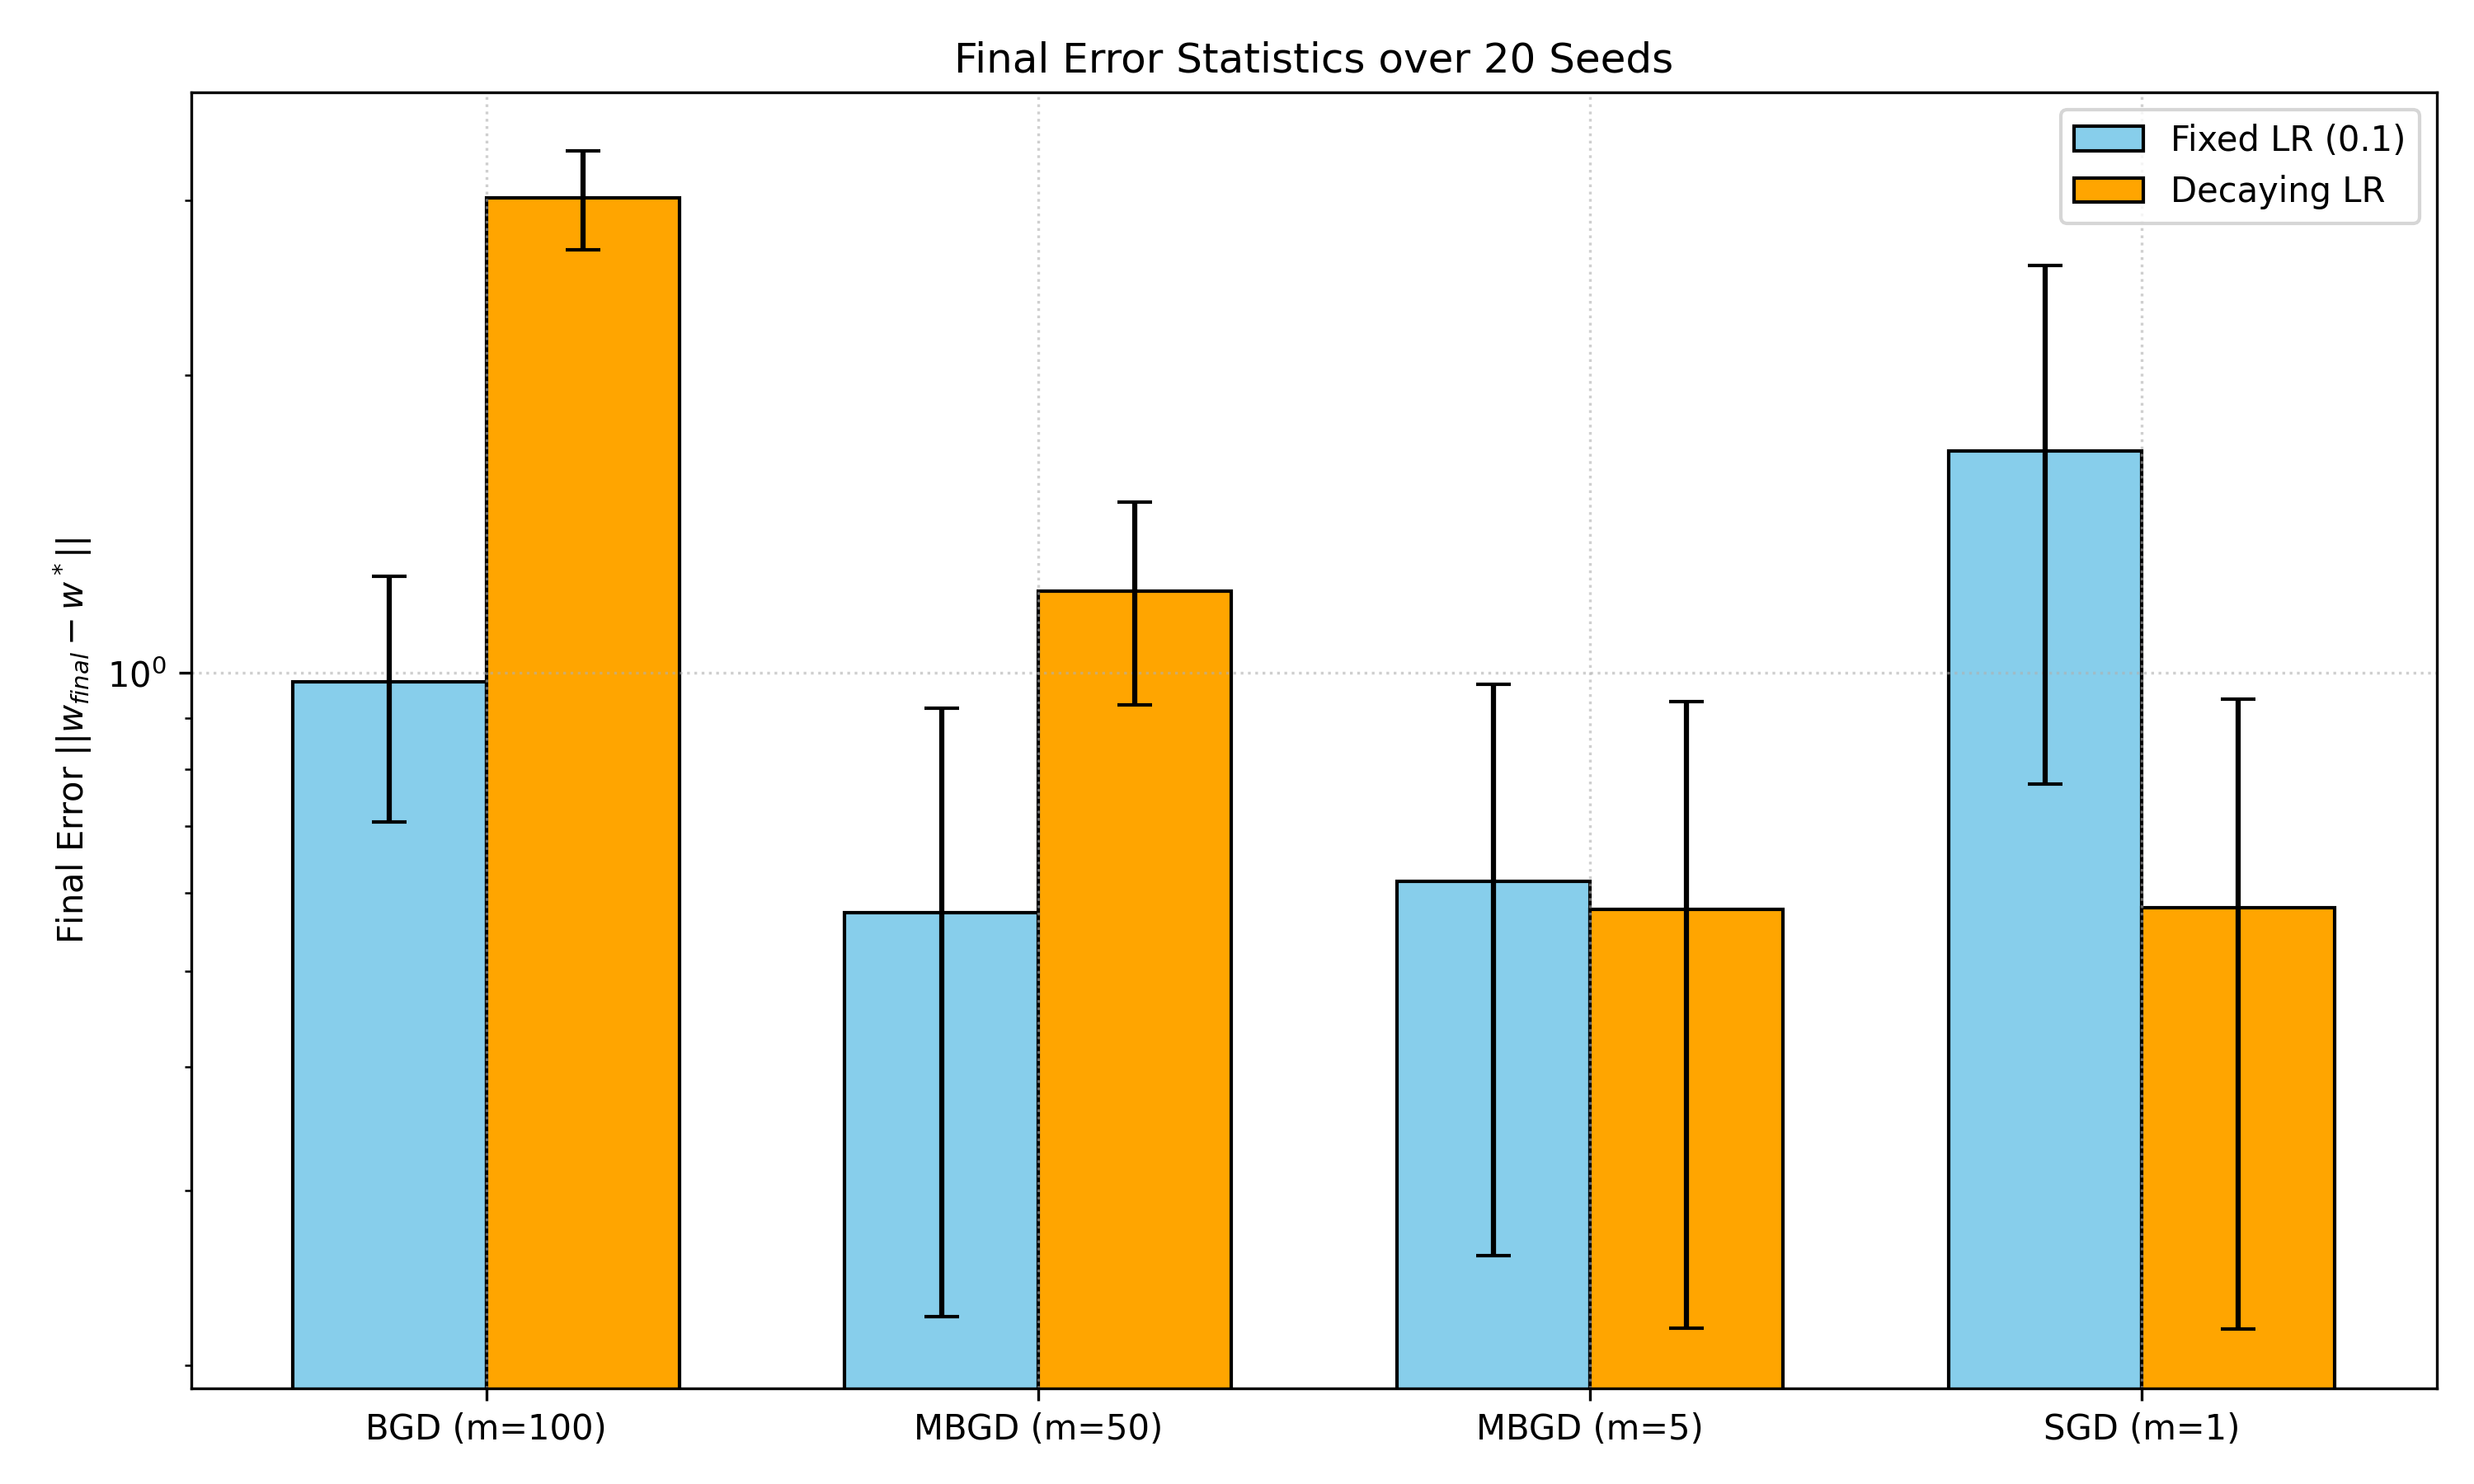
\includegraphics[width=0.75\textwidth]{exp3/results/task4_statistical_comparison.png}
\caption{20个随机种子下不同算法与学习率的最终误差统计}
\end{figure}

\paragraph{2. 异常样本（Outliers）敏感度分析}
\textbf{实验设计}：在 100 个样本中，有 95 个样本服从均匀分布 $U([-10, 10]^2)$，另外 5 个样本为异常值，固定在 $(50, 50)$。
\begin{itemize}
\item 此时无异常样本的真实分布均值为 $(0,0)$。
\item 含有异常样本的数据集样本均值被拉偏至 $[2.0318, 2.0281]$。
\end{itemize}

\textbf{实验结果}：
在含有异常值的数据集下，各优化算法的参数轨迹与误差收敛曲线如下：

\begin{figure}[H]
\centering
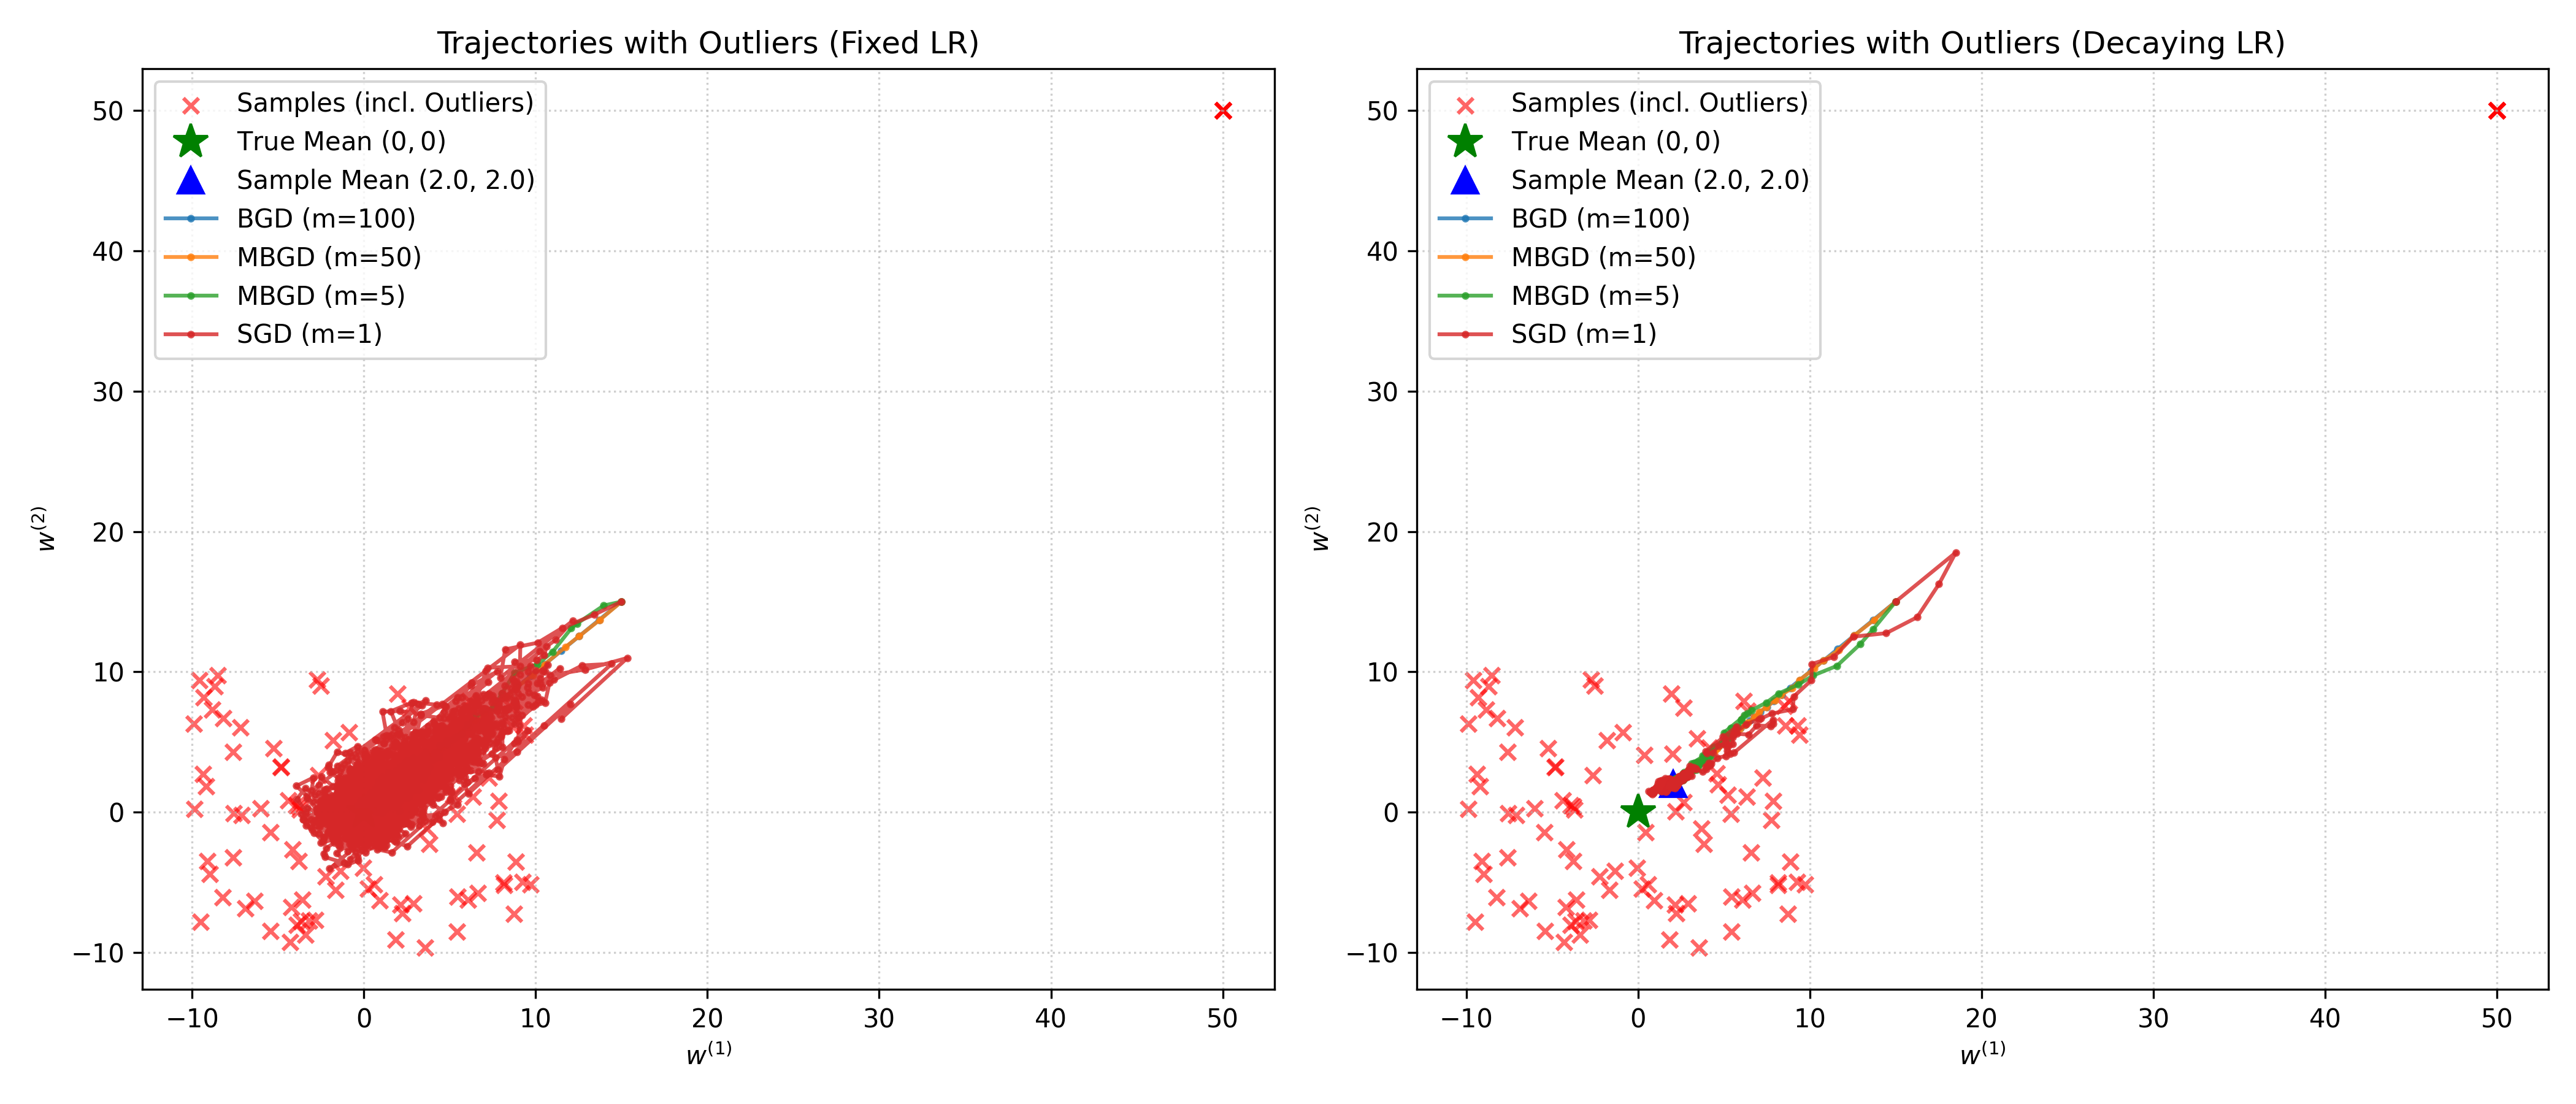
\includegraphics[width=0.75\textwidth]{exp3/results/task4_outlier_trajectories.png}
\caption{含异常样本(Outliers)下的优化轨迹比较}
\end{figure}
\begin{figure}[H]
\centering
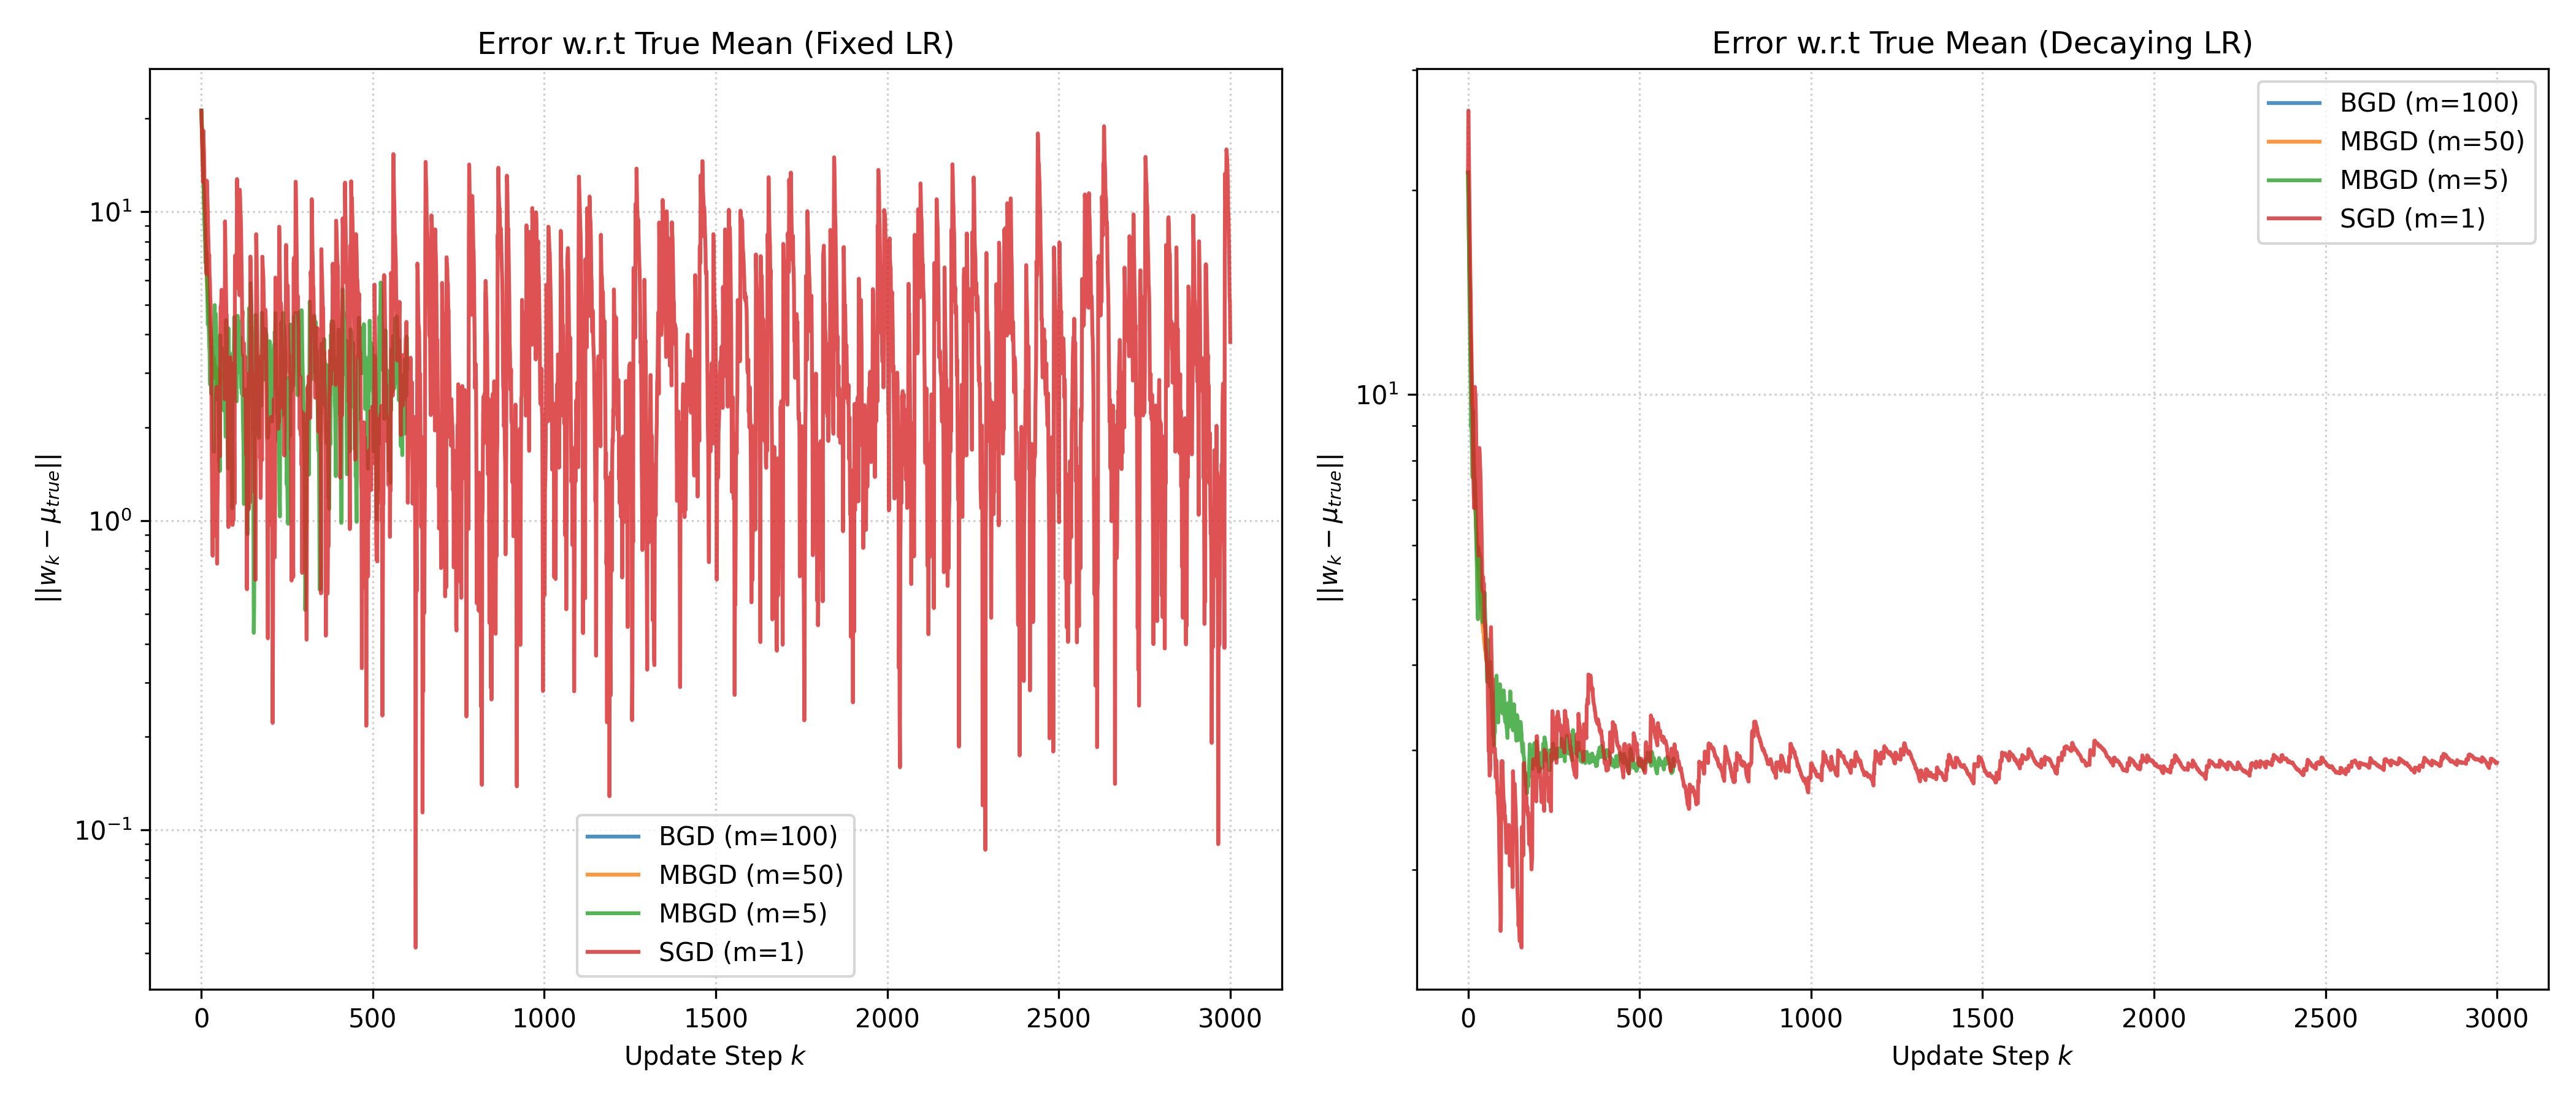
\includegraphics[width=0.75\textwidth]{exp3/results/task4_outlier_errors.png}
\caption{含异常样本(Outliers)下的误差曲线比较}
\end{figure}

\paragraph{思考题}



\textbf{问题 1：记录多随机种子的最终误差统计，并分析随机性对实验结论的影响。}


\answerlabel 
根据 20 个随机种子统计出的均值和标准差数据，有以下关键结论：
\begin{enumerate}
\item \textbf{固定学习率（Fixed LR）下}：
\item BGD 表现出中等的平均误差（0.9797），但方差极低（标准差 0.2717）。因为 BGD 在每个 epoch 中完全消除了数据采样的随机性，其收敛轨迹是确定性的，误差仅来源于样本均值本身与真实期望的偏差。
\item MBGD ($m=5, 50$) 获得了比 BGD 更低的平均误差（约 0.57-0.61），且表现出较好的稳定性。这是因为小批量引入的适当随机噪声在非凸/凸优化中可以作为正则化，避免过早陷入局部偏置或对特定分布过拟合。
\item SGD ($m=1$) 在固定学习率下平均误差最大（1.6764），且标准差极高（0.9037）。这是由于在固定步长下，单样本的高梯度方差使 SGD 无法平滑点收敛，参数在最后阶段仍在大范围内无规则跃迁。
\item \textbf{衰减学习率（Decaying LR）下}：
\item BGD 平均误差最高（3.0191）。原因是在 30 个 epochs 中，BGD 总共仅更新了 30 次参数，而其学习率随着步数快速衰减，导致其在后期更新幅度太小，还未充分接近最优值就已“冻结”（收敛太慢）。
\item SGD 和 MBGD（$m=5$）的平均最终误差约为 0.57。两者在 30 个 epochs 内具有较多参数更新次数；同时，衰减学习率减弱了训练后期的随机波动，因此在本次设置下得到较低误差。
\item \textbf{随机性对结论的影响}：
\item 单次实验（如任务 3 的单次运行）可能由于样本随机采样的特异性（例如生成了更容易收敛或存在偏差的样本）导致异常结果。例如，在单次实验中 MBGD 的误差可能偶尔低于或高于 SGD，这无法作为算法优劣的定性证据。
\item 通过 20 次独立重复实验进行均值与标准差统计，可以排除个体随机样本带来的偶发性偏差。统计分析表明，在有限 epoch 下，\textbf{衰减学习率对 SGD/小批量 MBGD 是必须的}，而\textbf{对于更新次数极少的 BGD 而言，过快衰减的学习率反而会严重阻碍其收敛}。
\end{enumerate}

\paragraph{2. 异常样本对 SGD 与 BGD 敏感程度的定性与定量分析}
根据任务 4 的异常值（Outlier）实验：
\begin{itemize}
\item \textbf{BGD 的敏感度}：
  BGD 每次更新使用全部样本的平均梯度。加入异常样本后，样本均值由 $(0,0)$ 移至约 $[2.03,2.02]$，因此经验损失的最优点也随之移动。BGD 轨迹较平滑，但最终位置受到异常样本引起的系统性偏移；衰减学习率设置下的剩余误差还包含训练轮数不足造成的未完全收敛部分。
\item \textbf{SGD 的敏感度}：
  SGD 每次随机挑选一个样本。在优化轨迹中，当 SGD 遇到那 95\% 的正常样本时，参数沿着指向 $(0,0)$ 的方向平稳行进；而\textbf{一旦随机抽样到那 5\% 的异常样本 $(50,50)$ 时，由于该样本提供的梯度极其巨大，SGD 的参数会被瞬间“踢飞”，在轨迹图上产生剧烈的突变跳跃（Spike）}（可参见 \texttt{task4\_outlier\_trajectories.png} 中 SGD 紫色线的巨大折线突变）。
\item \textbf{总结对比}：
\item \textbf{BGD 对异常样本的敏感性表现为“隐式系统偏差”}：它的轨迹非常稳定平滑，但最终收敛点会因为异常样本而发生严重偏移，缺乏鲁棒性。
\item \textbf{SGD 对异常样本的敏感性表现为“显式瞬态抖动”}：它的轨迹在遇到异常样本时会发生剧烈震荡，但如果配合合理的衰减步长，由于异常值样本出现概率低且步长在衰减，它在大部分时间仍受占主导地位的正常样本吸引，最终收敛点仍然能够非常接近正常分布的期望，甚至比 BGD 具有更好的某种“抗偏差”鲁棒性（例如在衰减学习率下，SGD 最终点到拉偏后样本均值的误差仅为 0.00177）。
\end{itemize}

\subsection{核心代码与分析}

\subsubsection{均值增量更新算法核心实现}
在 \texttt{task1\_sample\_mean.py} 中，增量均值更新根据数学公式 $w_k = w_{k-1} - \frac{1}{k}(w_{k-1} - x_k)$ 实现。代码如下：

\begin{lstlisting}[language=python]
# 增量估计核心迭代
w_2d = np.zeros(2)  # 初始化估计值 w_0 = [0, 0]
for k in range(1, N_2d + 1):
    x = samples_2d[k-1]  # 获取当前第 k 个样本（索引为 k-1）
    # 增量更新公式，步长为 1/k
    w_2d = w_2d - (1.0 / k) * (w_2d - x)
    incremental_means_2d[k-1] = w_2d.copy()
\end{lstlisting}
\begin{itemize}
\item \textbf{输入}：当前样本 \texttt{x}，步数 \texttt{k}。
\item \textbf{输出}：更新后的估计参数向量 \texttt{w\_2d}。
\item \textbf{物理含义}：每次新样本 $x_k$ 带来一个误差修正方向 $(w_{k-1} - x_k)$，以 $\frac{1}{k}$ 的权重逐渐衰减地叠加到原有估计值上，从而在不保存历史数据的前提下保持实时期望估计。
\end{itemize}
\subsubsection{统一接口下的 BGD、MBGD、SGD 梯度更新}
在 \texttt{task3\_stochastic\_optimization.py} 中，通过灵活配置 \texttt{batch\_size} 统一实现了 BGD、MBGD 与 SGD，并且支持固定与衰减两种学习率：

\begin{lstlisting}[language=python]
def run_optimizer(samples, method, batch_size, lr_type, lr_0=0.1, epochs=30, w_0=np.array([15.0, 15.0])):
    N = len(samples)
    w = w_0.copy()
    traj_step = [w.copy()]
    traj_epoch = [w.copy()]
    update_counter = 0  # 全局更新步数计数器 k
    
    for epoch in range(epochs):
        # 1. 随机打乱样本顺序以满足随机近似的条件
        indices = np.arange(N)
        if method in ['SGD', 'MBGD']:
            np.random.shuffle(indices)
        
        # 2. 分批更新参数
        for start_idx in range(0, N, batch_size):
            end_idx = min(start_idx + batch_size, N)
            batch_indices = indices[start_idx:end_idx]
            batch_samples = samples[batch_indices]
            
            # 3. 计算当前 mini-batch 上的样本平均梯度
            # \nabla J_B(w) = w - \bar{x}_B
            grad = w - np.mean(batch_samples, axis=0)
            
            # 4. 动态计算学习率
            if lr_type == 'fixed':
                lr = lr_0
            elif lr_type == 'decaying':
                lr = lr_0 / (1.0 + 0.05 * update_counter)
                
            # 5. 参数更新
            w = w - lr * grad
            update_counter += 1
            
            traj_step.append(w.copy())
        traj_epoch.append(w.copy())
        
    return np.array(traj_step), np.array(traj_epoch)
\end{lstlisting}
\begin{itemize}
\item \textbf{接口设计}：通过控制 \texttt{batch\_size}：
\item \texttt{batch\_size = 100} ($N$) 即为 \textbf{BGD}；
\item \texttt{batch\_size = 5} 或 \texttt{50} 即为 \textbf{MBGD}；
\item \texttt{batch\_size = 1} 即为 \textbf{SGD}。
\item \textbf{学习率衰减控制}：\texttt{update\_counter} 记录全局梯度更新 of parameter. 对于 SGD，每个 epoch 更新 100 次，学习率衰减较快，能快速压低后期噪声；而对于 BGD，每个 epoch 仅更新 1次，学习率衰减缓慢，但由于总更新步数太少（仅 30 步），容易受到前期慢速收敛的限制。
\end{itemize}
\subsection{总结与体会}

\begin{enumerate}
\item \textbf{增量更新的存储优势}：
   增量均值与直接平均的最大差异仅为浮点误差量级，同时将历史样本存储需求降为 $O(1)$。该递推形式也为后续 TD 更新和 Q-learning 的在线更新提供了直接参照。
\item \textbf{Robbins-Monro 步长条件的实践印证}：
   收敛曲线显示，常数步长在真实值附近持续波动，$1/k^2$ 因累计修正量有限而提前停滞，$1/k$ 则继续纠偏并逐步抑制噪声。步长选择需要同时满足持续纠偏和降低随机扰动两项要求。
\item \textbf{计算效率与梯度的权衡}：
   BGD 的单步方向稳定但每次更新使用全部样本；SGD 单步成本低但轨迹波动较大；MBGD 在本实验中兼顾了更新频率与梯度方差。实际选择仍需结合样本规模、计算预算和允许的稳态误差。
\end{enumerate}

\newpage
\section{时序差分学习}

\subsection{实验目的与要求}
\begin{enumerate}
\item 理解时序差分学习（Temporal-Difference Learning）的核心思想：掌握 TD目标、TD误差和 bootstrapping更新。
\item 掌握TD(0)策略评估方法：能够在给定策略下估计状态价值函数，并与Monte Carlo策略评估进行对比。
\item 掌握Sarsa与n-step Sarsa：能够实现同策略动作价值学习，并分析n-step目标在TD与MC之间的折中。
\item 掌握Q-learning：能够实现异策略TD控制，并理解其与Sarsa在TD目标和策略性质上的区别。
\item 培养强化学习实验分析能力：能够绘制RMSE、累计奖励、成功率、到达目标步数和最终策略图，并给出合理解释。
\end{enumerate}
\subsection{实验内容与设计}

\subsubsection{公共环境与评价指标}

四个任务均使用 $5\times5$ GridWorld，普通移动与撞墙奖励为 $-1$，到达右下角目标奖励为 $+1$，折扣因子为 $\gamma=0.9$。策略评估任务使用均匀随机策略；控制任务使用 $\epsilon$-greedy 行为策略。评估指标包括 RMSE、累计奖励、成功率、到达目标步数和最终贪心策略。

\subsubsection{任务 1--2：基准价值与 TD(0) 评估设计}

任务 1 通过动态规划迭代求解随机策略的基准价值，作为后续 RMSE 的参照。任务 2 在相同策略下比较 TD(0) 与 First-Visit MC，并测试固定步长 $\alpha=0.05$、$\alpha=0.1$ 和访问次数衰减步长。所有方法使用相同环境和评价基准，以区分自举更新与完整回合更新的差异。

\subsubsection{任务 3：Sarsa 与 n-step Sarsa 设计}

使用相同初始动作值和行为策略，比较 $n=1,3,5$ 的 n-step Sarsa。记录累计奖励、成功率、到达目标步数和最终策略，重点分析 $n$ 增大后更新目标在偏差与方差之间的变化。

\subsubsection{任务 4：同策略与异策略控制设计}

在相同随机种子和超参数下比较 Sarsa 与 Q-learning。两种算法均使用 $\epsilon$-greedy 行为策略与环境在线交互，记录累计奖励、成功率、到达目标步数和最终贪心策略，用于分析同策略与异策略 TD 目标对学习过程的影响。




\subsection{实验过程、结果与分析}

\subsubsection{任务 1：实验环境与基准价值}

本任务构建 $5\times5$ GridWorld 环境并通过动态规划策略评估（贝尔曼期望方程迭代）计算均匀随机策略 $\pi$ 的精确状态价值 $v_\pi$，作为后续无模型（TD 与 MC）算法误差评估的基准。

TD 误差定义为 $\delta_t=R_{t+1}+\gamma V(S_{t+1})-V(S_t)$，即单步自举目标与当前估计之差。由于该目标只需要当前奖励和下一状态的价值估计，TD 方法在 episode 尚未结束时即可更新；MC 方法则需要等待完整回合结束后计算实际回报。

\paragraph{环境设置}
本实验使用 $5 \times 5$ GridWorld 作为统一测试环境，其状态、动作、转移与奖励规则如下：
\begin{itemize}
\item \textbf{状态空间 $S$}：$5 \times 5$ 的网格坐标 $(r, c)$，其中 $r, c \in \{0, 1, 2, 3, 4\}$。右下角状态 $(4, 4)$ 为终止目标状态（Goal State）。
\item \textbf{动作空间 $A$}：每个状态包含四个动作 $\{0: \text{Up}, 1: \text{Down}, 2: \text{Left}, 3: \text{Right}\}$。
\item \textbf{状态转移}：动作执行为确定性转移。若代理人撞墙（即试图移出网格边界），则保持在原地。
\item \textbf{奖励设置}：到达终止目标状态 $(4,4)$ 的转移奖励为 $+1.0$，并结束当前 episode；普通移动与撞墙移动的奖励均为 $-1.0$。
\item \textbf{折扣因子 $\gamma$}：固定为 $0.9$。
\end{itemize}

\begin{figure}[H]
\centering
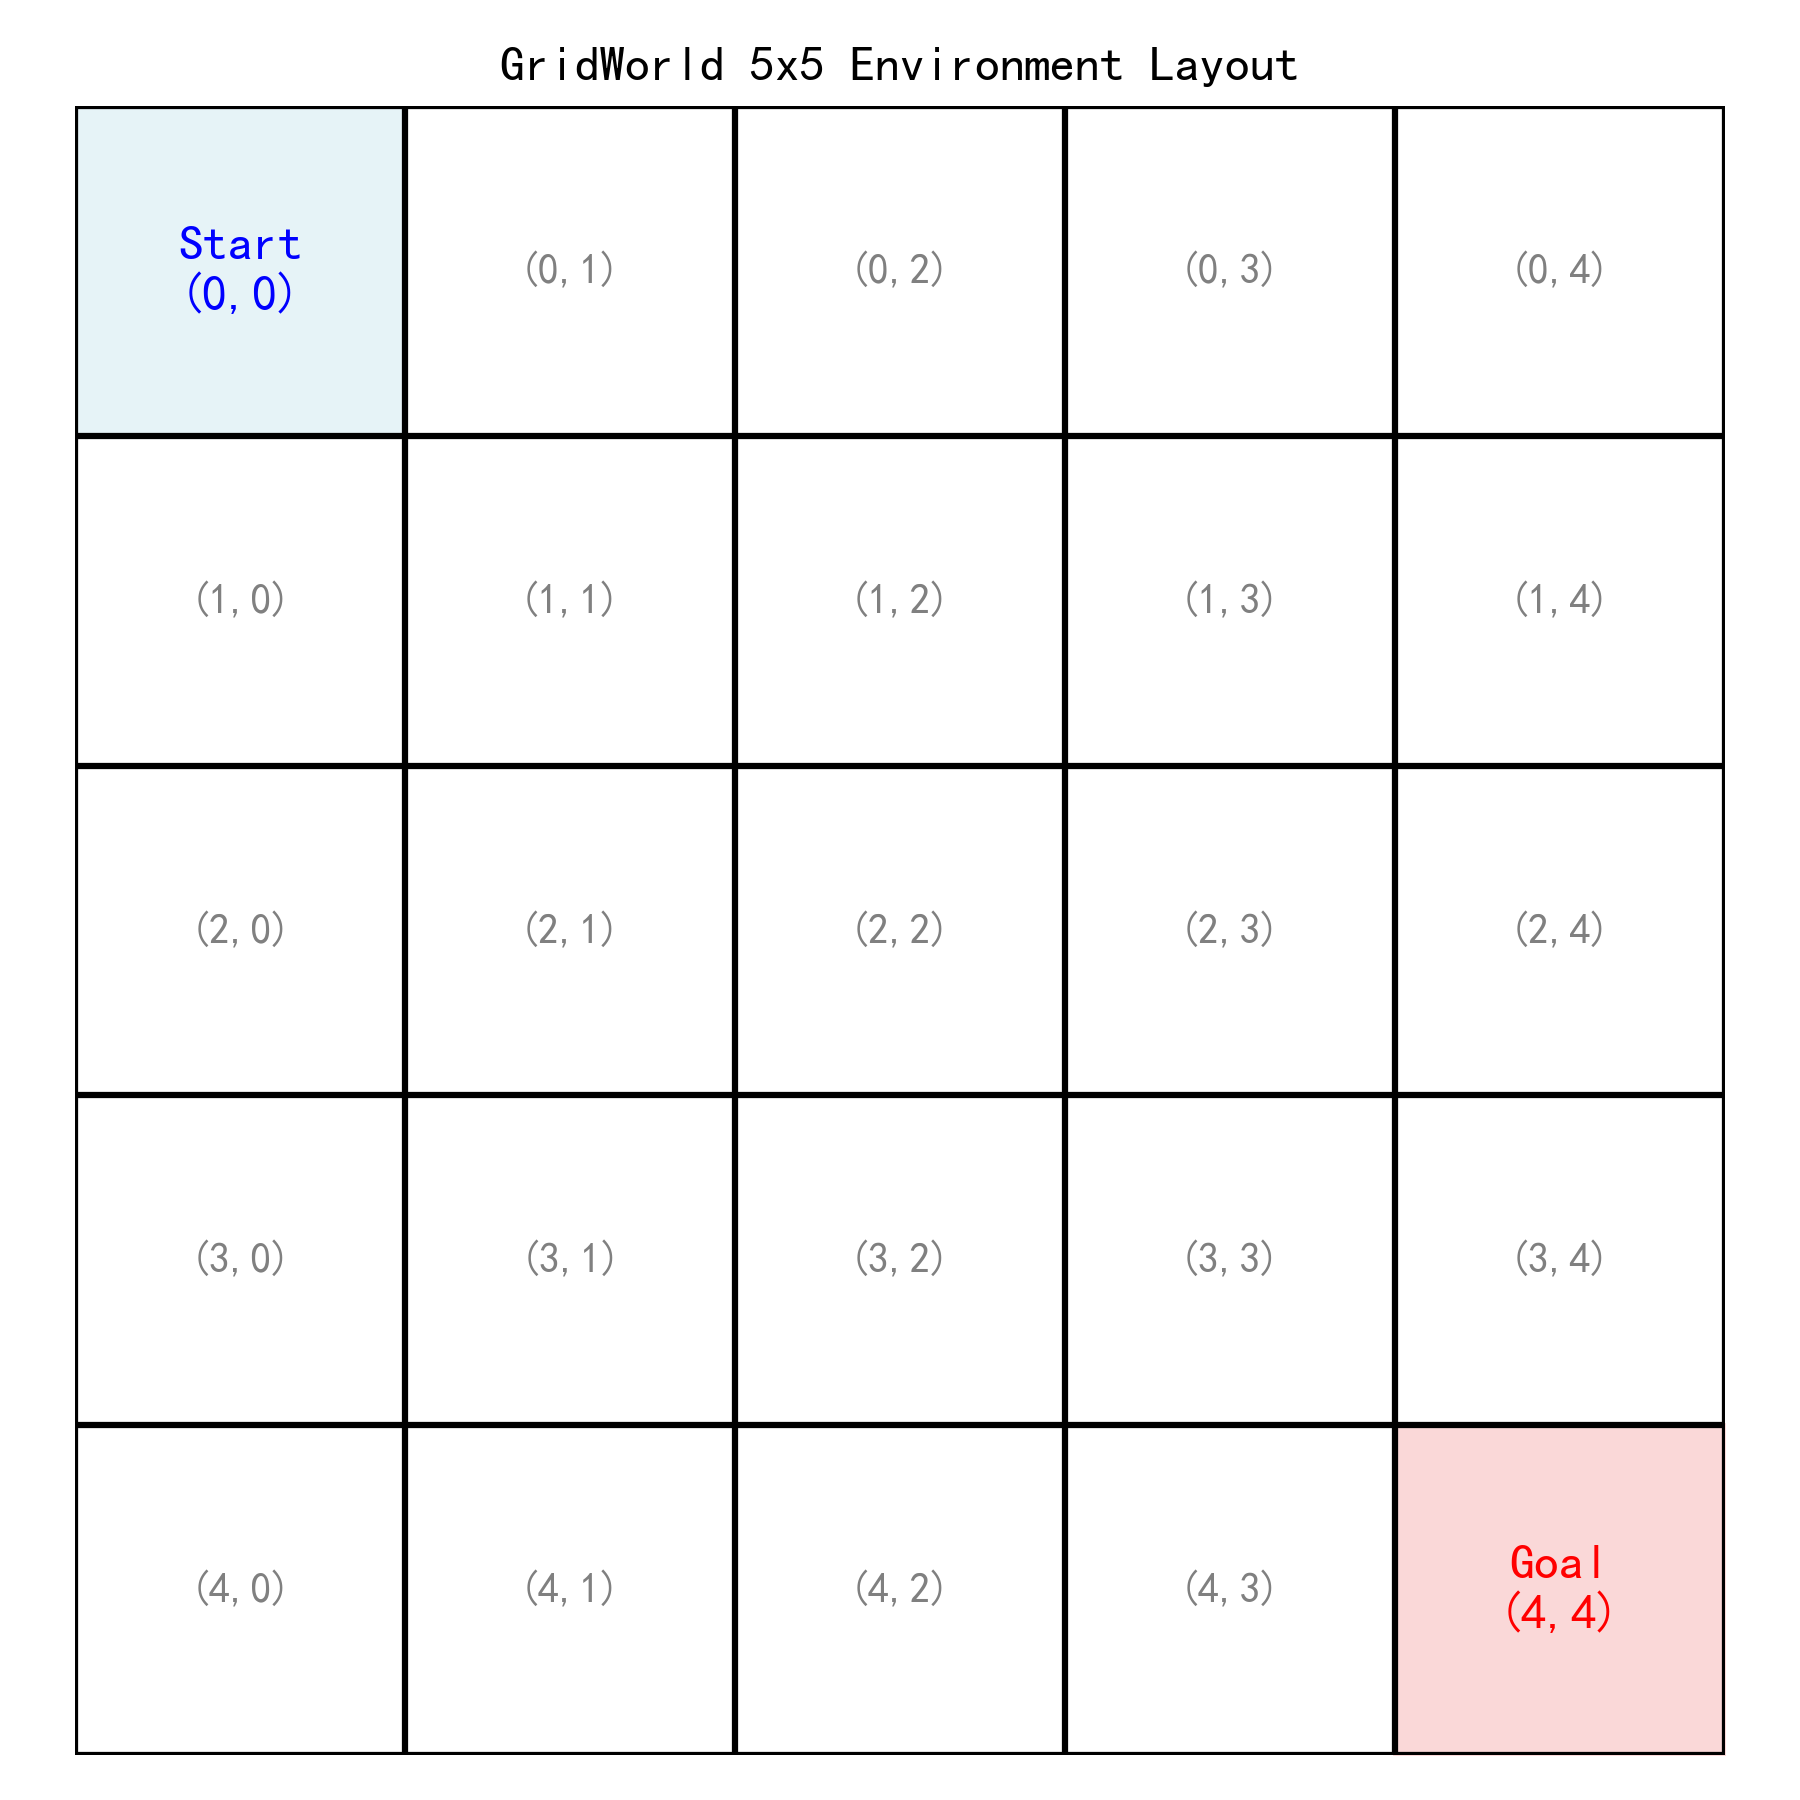
\includegraphics[width=0.5\textwidth]{exp4/results/gridworld_schematic.png}
\caption{GridWorld Layout}
\end{figure}

\paragraph{基准价值计算}
为了精确计算后续无模型（Model-free）评估算法的 RMSE 误差，我们需要先通过动态规划（DP）求解贝尔曼期望方程，获得均匀随机策略 $\pi$（每个非终止状态下四个动作的选择概率均为 $0.25$）的精确状态价值 $v_\pi$。
贝尔曼期望方程展开式为：
$$v_\pi(s) = \sum_{a \in A} \pi(a|s) \left[ \mathcal{R}_s^a + \gamma \sum_{s' \in S} \mathcal{P}_{ss'}^a v_\pi(s') \right]$$
在确定性环境和均匀随机策略下，公式简化为：
$$v_\pi(s) = 0.25 \sum_{a=0}^{3} \left[ R(s, a) + \gamma v_\pi(s'(s, a)) \right]$$
其中终止状态 $v_\pi(4, 4) = 0.0$。

动态规划策略评估在第 201 次迭代满足阈值 $10^{-10}$，求得的基准状态价值矩阵如下：

\begin{table}[H]
\centering
\begin{tabular}{cccccc}
\toprule
$V_\pi$ 行\textbackslash\{\}列 & 0 (col) & 1 (col) & 2 (col) & 3 (col) & 4 (col) \\
\midrule
\textbf{0 (row)} & -9.7238 & -9.6624 & -9.5475 & -9.4063 & -9.2983 \\
\textbf{1 (row)} & -9.6624 & -9.5659 & -9.3729 & -9.1091 & -8.8784 \\
\textbf{2 (row)} & -9.5475 & -9.3729 & -8.9902 & -8.3831 & -7.7292 \\
\textbf{3 (row)} & -9.4063 & -9.1091 & -8.3831 & -6.9850 & -4.9170 \\
\textbf{4 (row)} & -9.2983 & -8.8784 & -7.7292 & -4.9170 & 0.0000 \\
\bottomrule
\end{tabular}
\end{table}

基准价值热力图如下：

\begin{figure}[H]
\centering
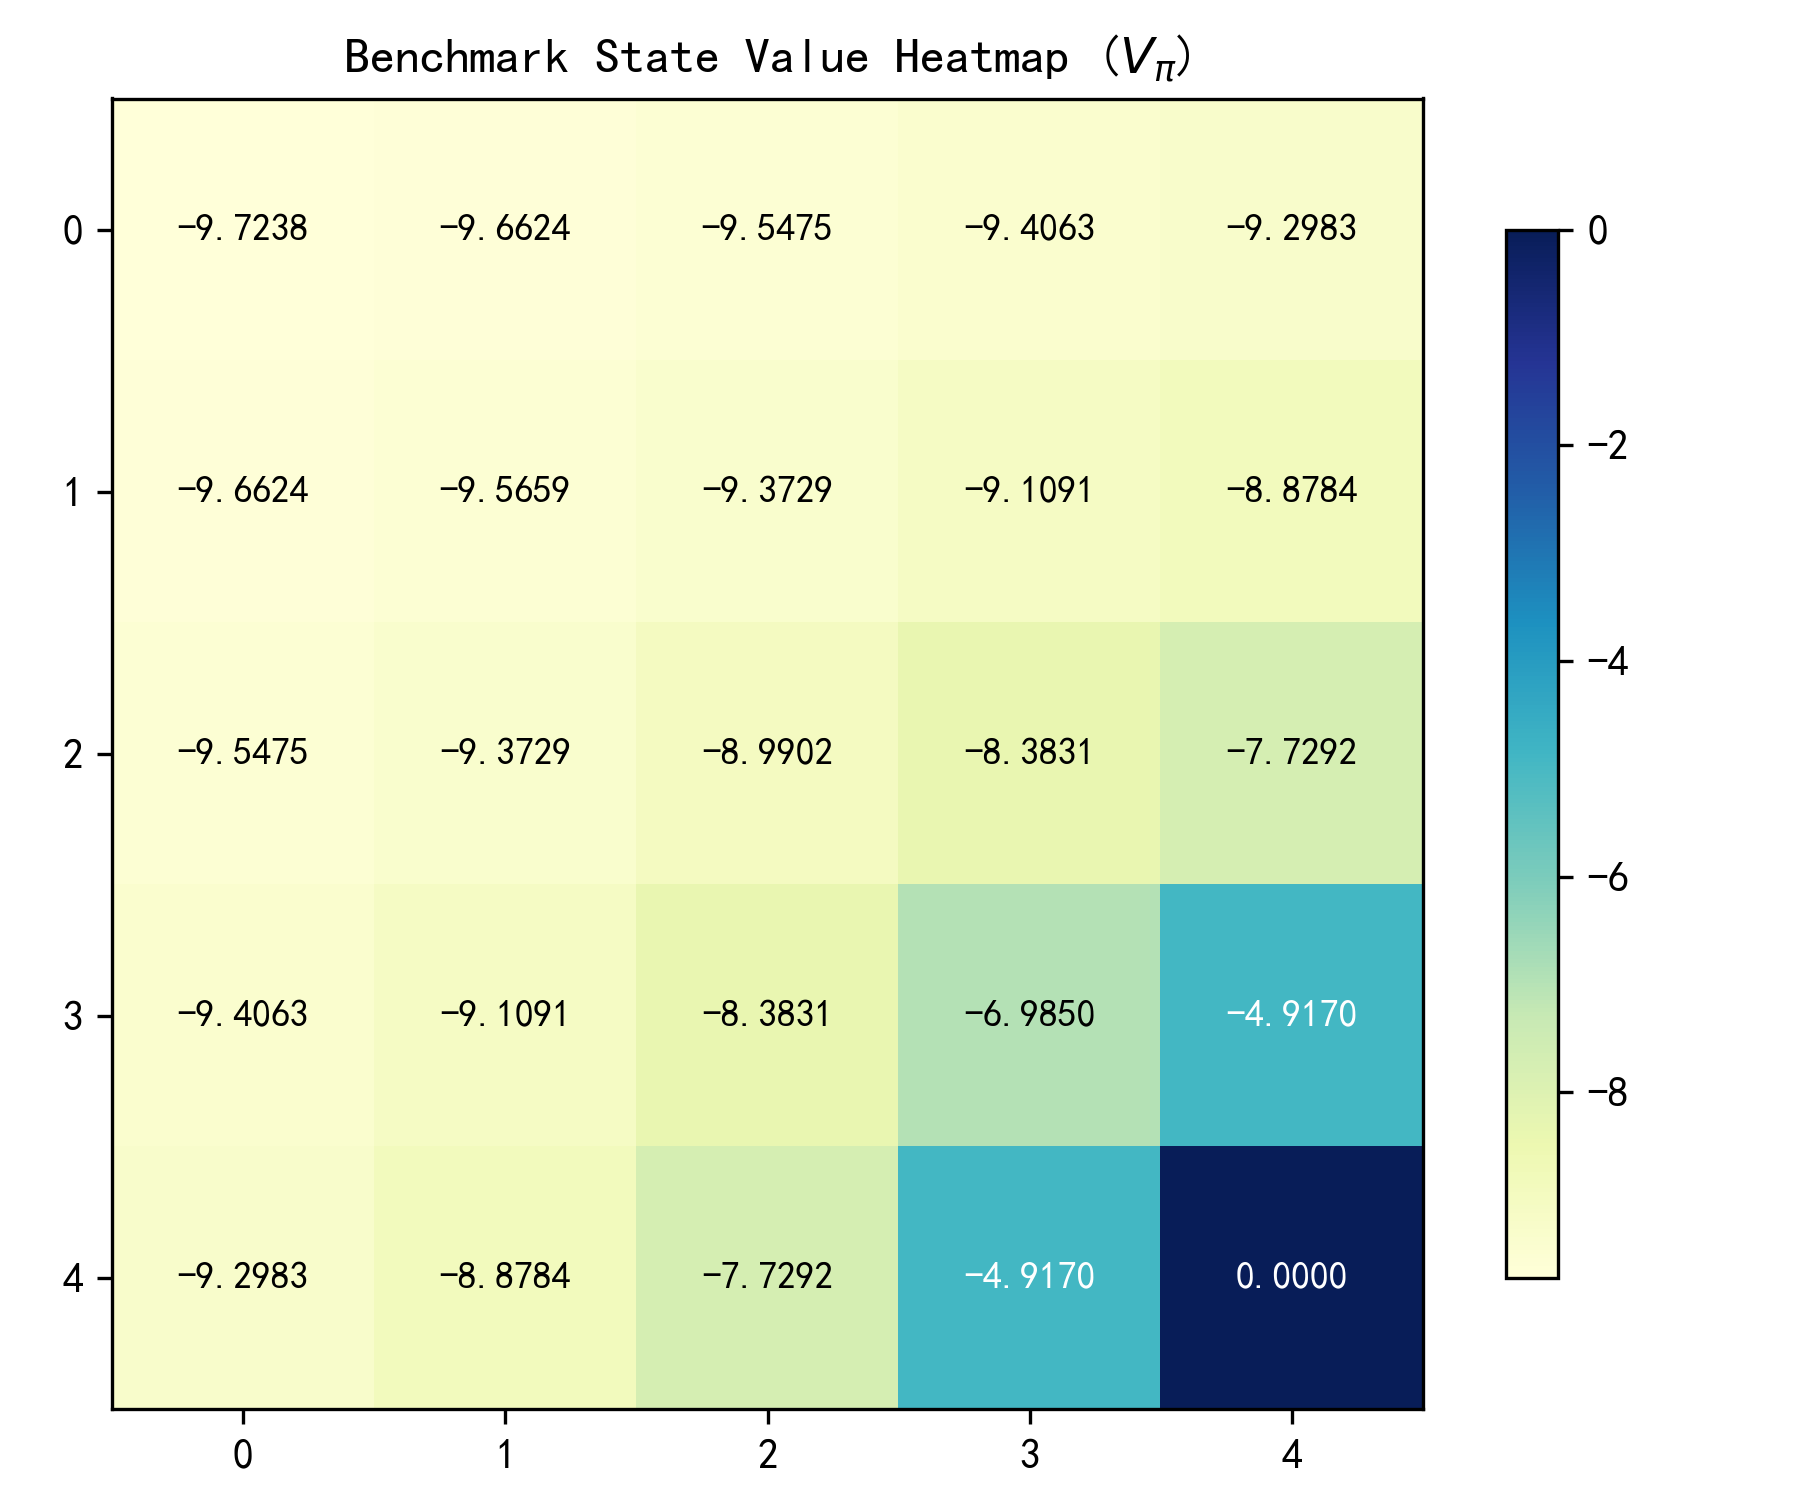
\includegraphics[width=0.5\textwidth]{exp4/results/dp_benchmark_heatmap.png}
\caption{DP Benchmark Heatmap}
\end{figure}

\paragraph{结果分析}
由于普通移动和撞墙均产生 $-1.0$ 奖励，均匀随机策略在到达目标前通常经历较长的随机游走，因此除终止状态外的基准价值均为负值。表中价值从左上角的 $-9.7238$ 逐步升高至目标附近的 $-4.9170$，说明距离目标较近的状态具有更短的期望到达时间。

\paragraph{思考题}



\question{问题：为什么需要基准价值函数？如果没有动态规划真值，还可以如何近似评估算法误差？}

\answerlabel 基准价值为误差计算提供统一参照。将估计值与 $v_\pi$ 比较，可以计算 RMSE 或最大绝对误差，从而在相同尺度下比较不同算法的收敛速度和最终精度。

无法通过动态规划获得真值时，可以采用以下近似评价方法：
\begin{enumerate}
\item 使用大量独立 Monte Carlo 回合计算经验平均回报，并报告置信区间；
\item 使用独立测试轨迹比较各估计函数对实际回报的预测误差；
\item 若环境模型可用于评估但不用于训练，则计算贝尔曼残差，检查估计值对贝尔曼方程的满足程度。
\end{enumerate}
这些指标只能作为近似依据，其中 Monte Carlo 估计仍受有限样本误差影响，贝尔曼残差较小也不等同于已获得精确真值。


\subsubsection{任务 2：TD(0) 与蒙特卡罗策略评估对比}

TD(0) 采用单步自举（Bootstrapping）：$V(S_t) \leftarrow V(S_t) + \alpha[R_{t+1} + \gamma V(S_{t+1}) - V(S_t)]$，每一步转移即可更新，方差小、数据利用率高。Monte Carlo 则等待整条 episode 结束后用累积折扣回报 $G_t$ 更新，方差大但估计无偏。本任务对比四种配置（三种 TD(0) + FV-MC）在 20 次独立 trial 下的 RMSE 收敛曲线。

本任务在上述 GridWorld 环境中对均匀随机策略 $\pi$ 进行评估。我们对比了四种配置：
\begin{enumerate}
\item \textbf{TD(0) 恒定步长 $\alpha = 0.05$}
\item \textbf{TD(0) 恒定步长 $\alpha = 0.1$}
\item \textbf{TD(0) 衰减步长 $\alpha_t = 1/N(s_t)$}
\item \textbf{First-Visit Monte Carlo (FV-MC) 策略评估}（采用递增均值形式更新，等价于学习率 $1/N(s)$）
\end{enumerate}

为了消除单次随机采样的噪声，实验运行了 20 次独立的 trial，每次 trial 包含 500 个 episode，各 episode 均随机选择非终止状态作为起点。

\paragraph{RMSE 收敛曲线对比}
RMSE 计算公式为：
$$\text{RMSE} = \sqrt{\frac{1}{25} \sum_{r=0}^{4} \sum_{c=0}^{4} (V[r, c] - V_\pi[r, c])^2}$$

下图展示了 20 次独立运行平均后的 RMSE 随 episode 数目的收敛曲线：

\begin{figure}[H]
\centering
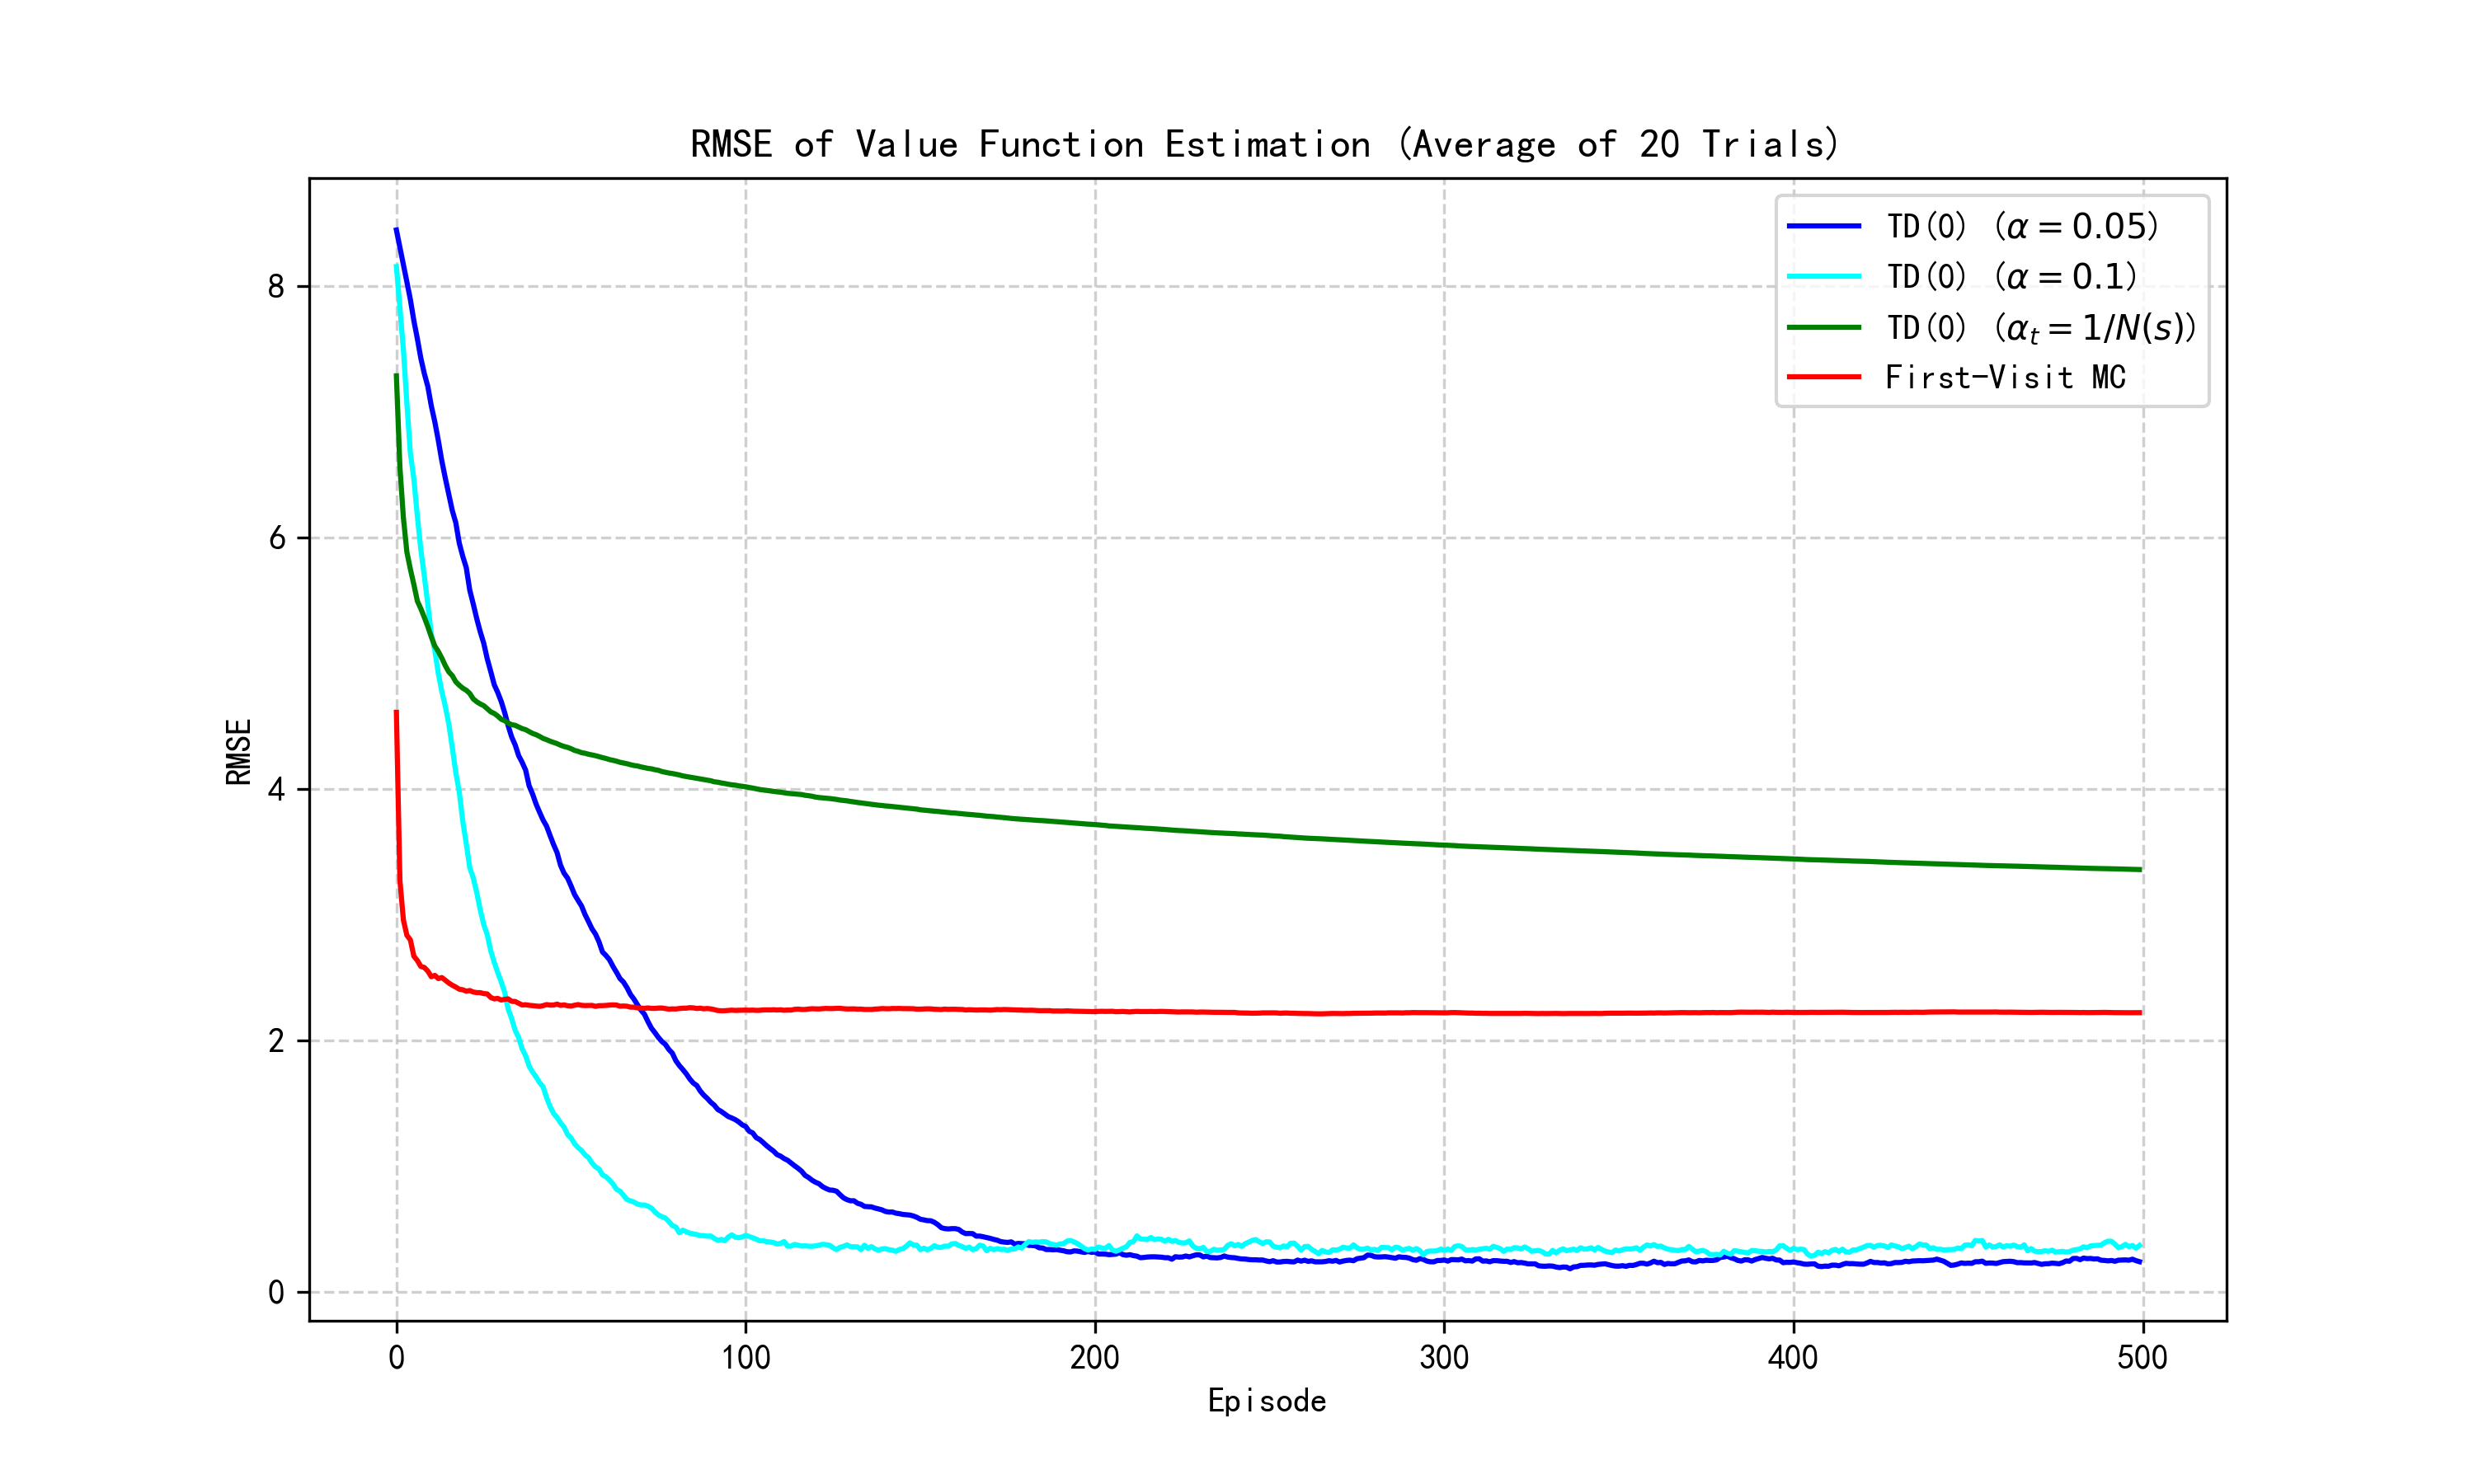
\includegraphics[width=0.7\textwidth]{exp4/results/rmse_comparison.png}
\caption{RMSE Comparison}
\end{figure}

\paragraph{估计状态价值热力图对比}
以下是第 0 次独立运行（Trial 0）结束时各方法估计出的状态价值热力图：

\begin{figure}[H]
\centering
\begin{minipage}{0.40\textwidth}
\centering
\textbf{TD(0) ($\alpha=0.05$)}\\[0.4em]
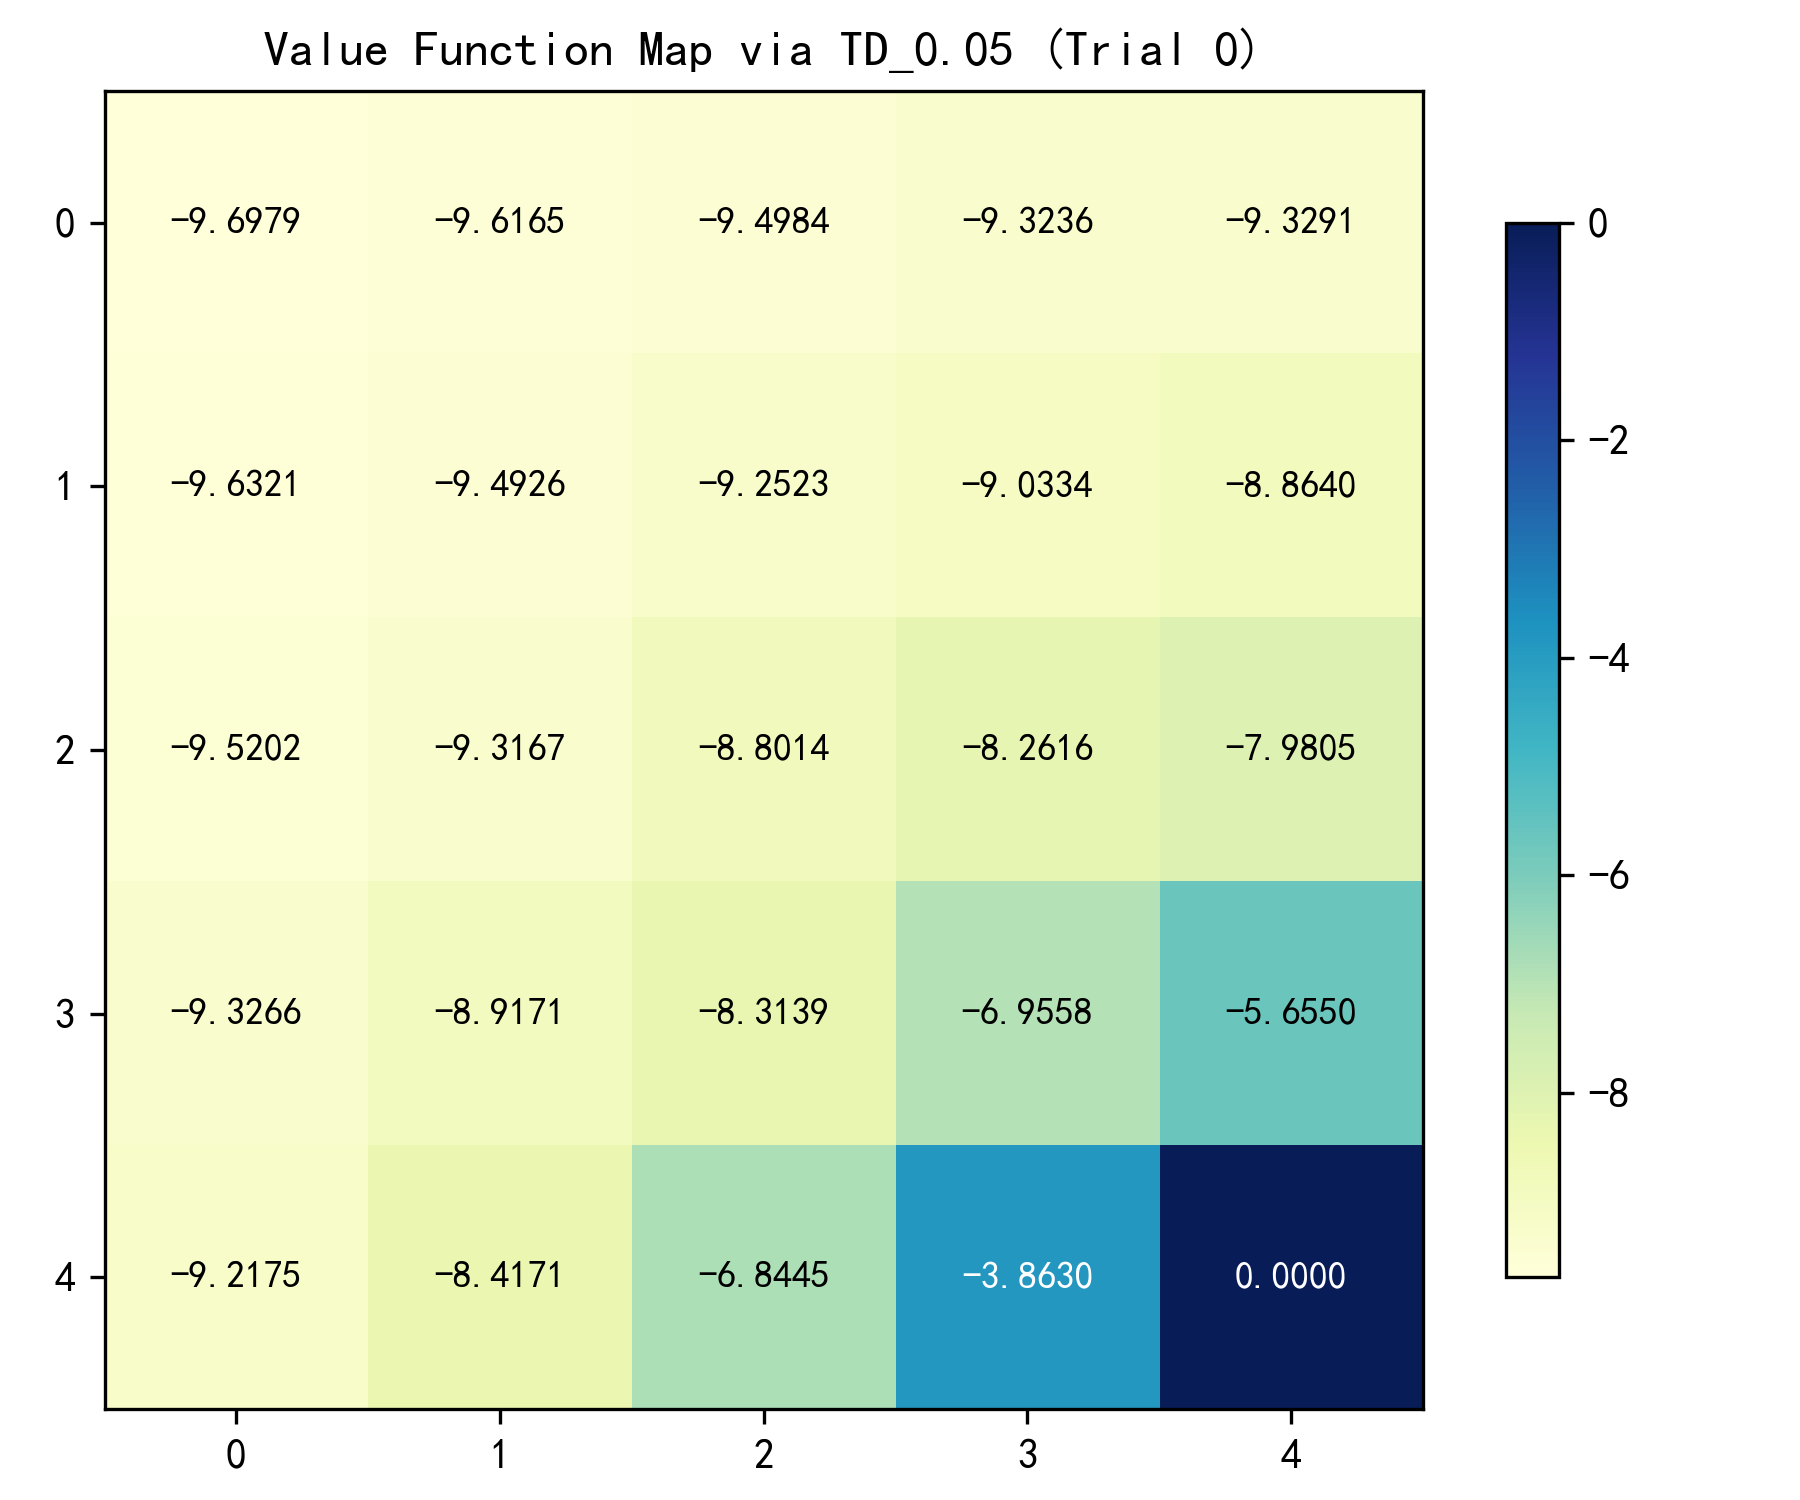
\includegraphics[width=\linewidth]{exp4/results/heatmap_TD_0.05.png}
\end{minipage}\hfill
\begin{minipage}{0.40\textwidth}
\centering
\textbf{TD(0) ($\alpha=0.1$)}\\[0.4em]
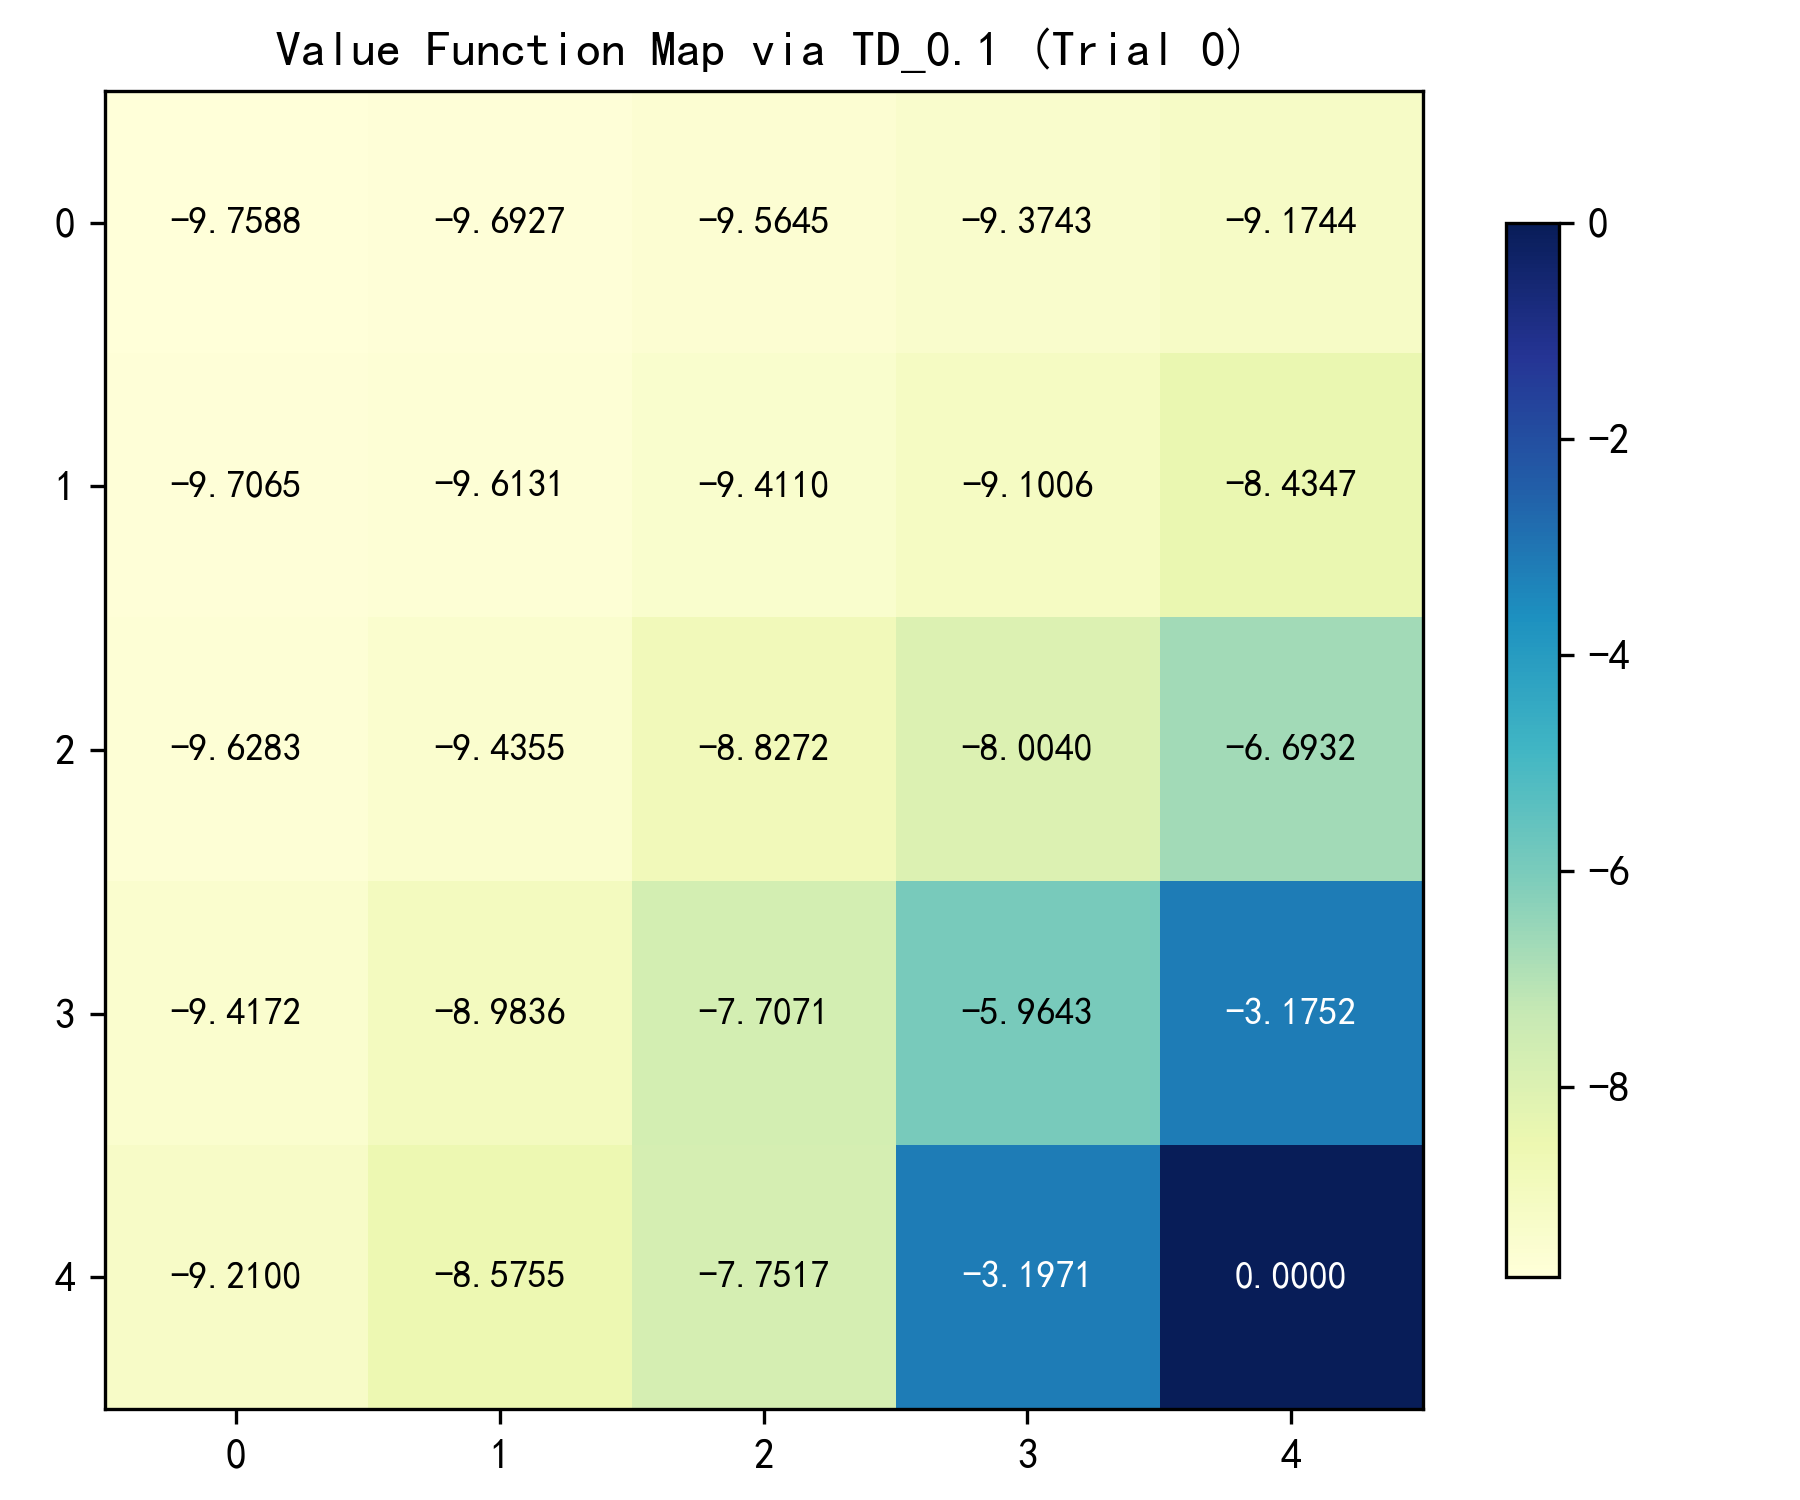
\includegraphics[width=\linewidth]{exp4/results/heatmap_TD_0.1.png}
\end{minipage}\\[0.8em]
\begin{minipage}{0.40\textwidth}
\centering
\textbf{TD(0) ($\alpha_t=1/N(s_t)$)}\\[0.4em]
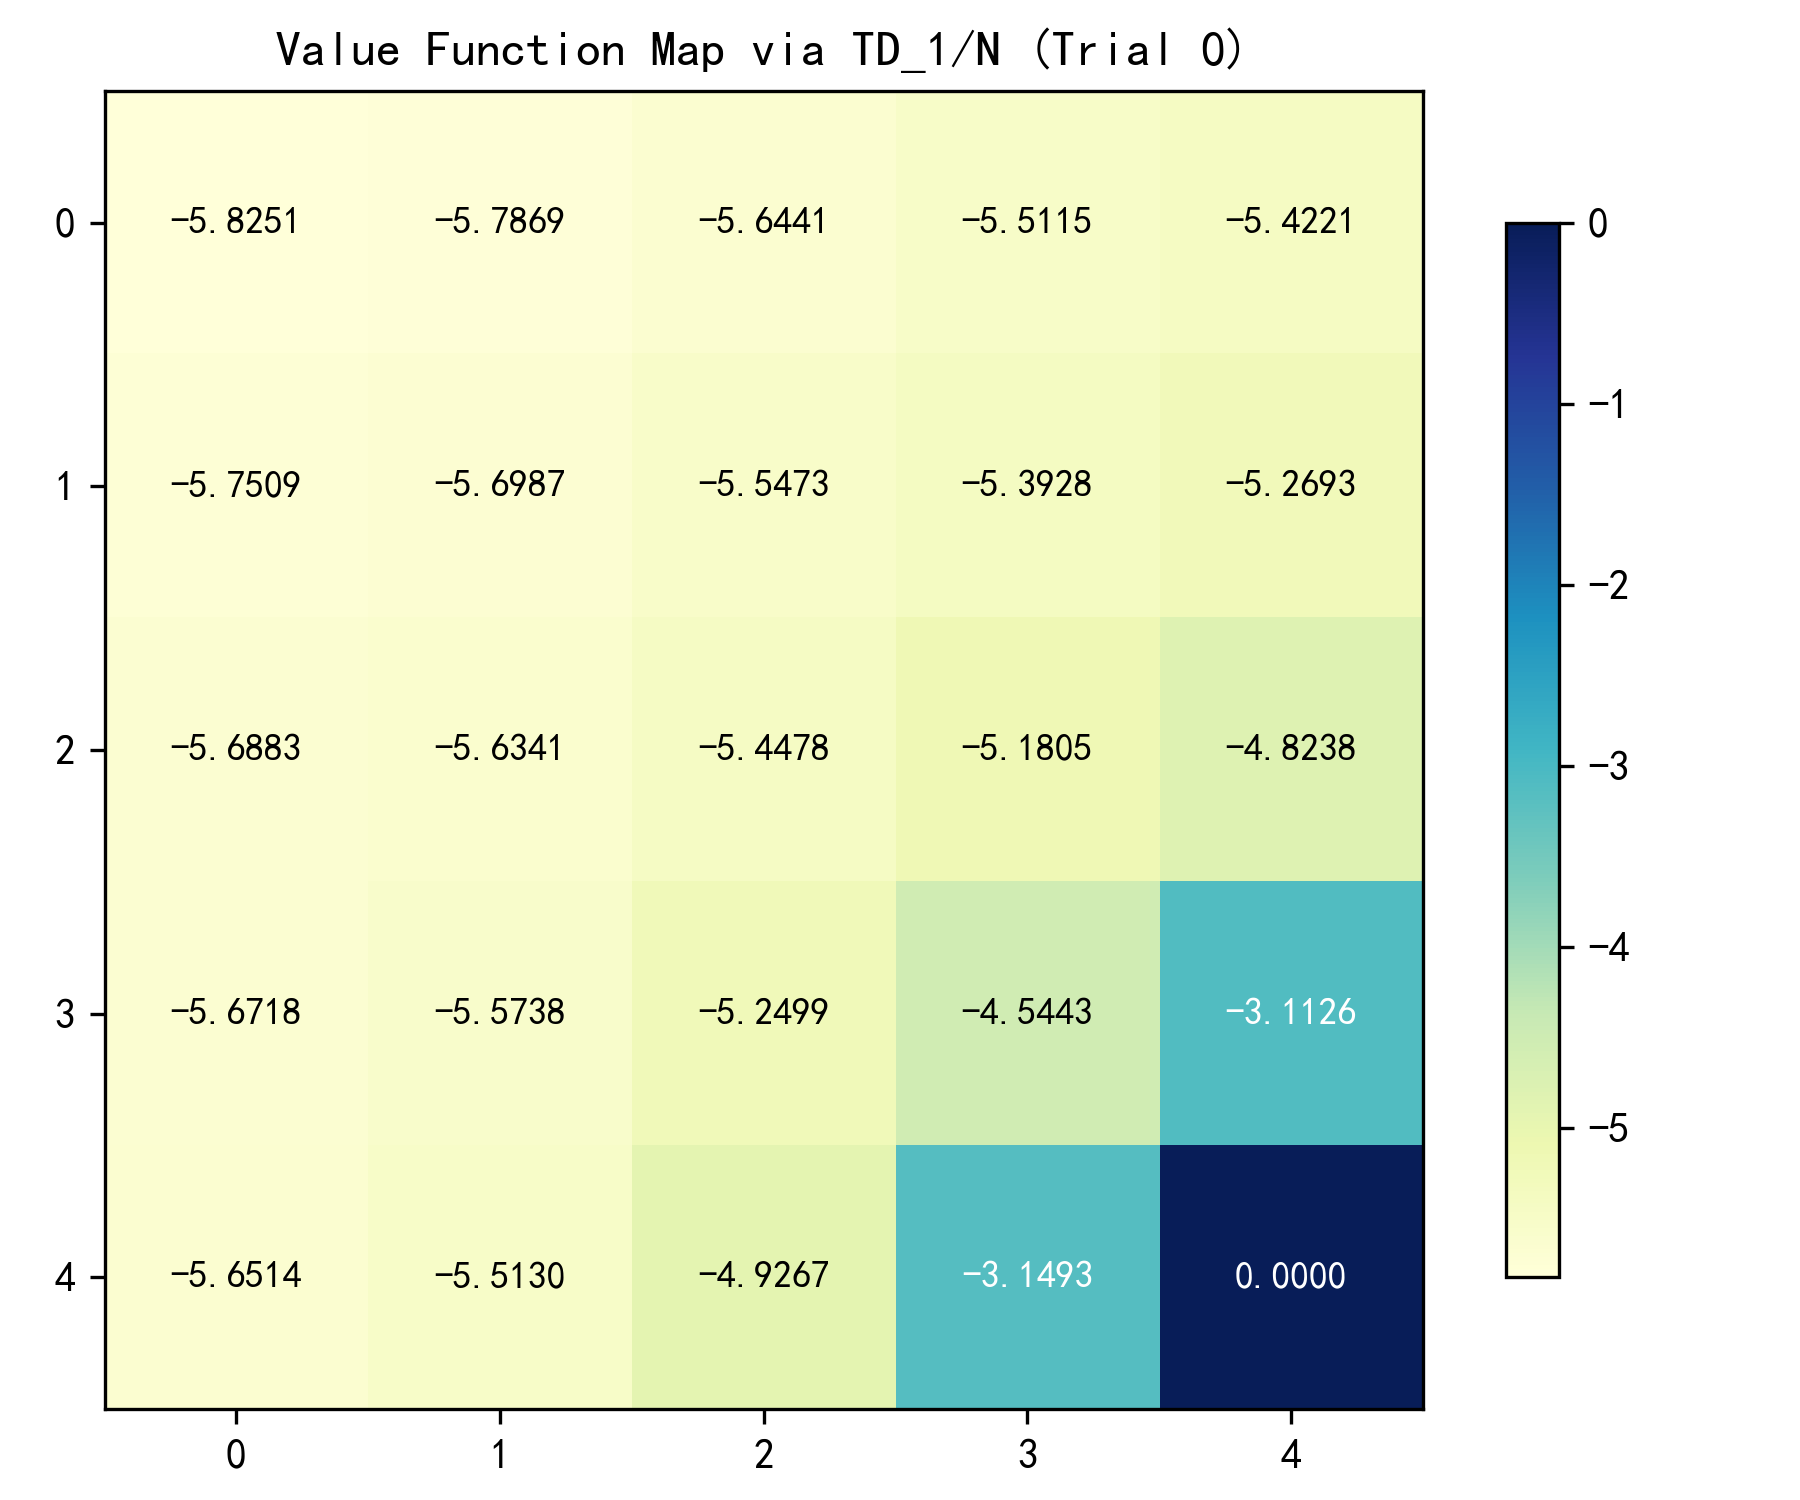
\includegraphics[width=\linewidth]{exp4/results/heatmap_TD_1_N.png}
\end{minipage}\hfill
\begin{minipage}{0.40\textwidth}
\centering
\textbf{First-Visit Monte Carlo}\\[0.4em]
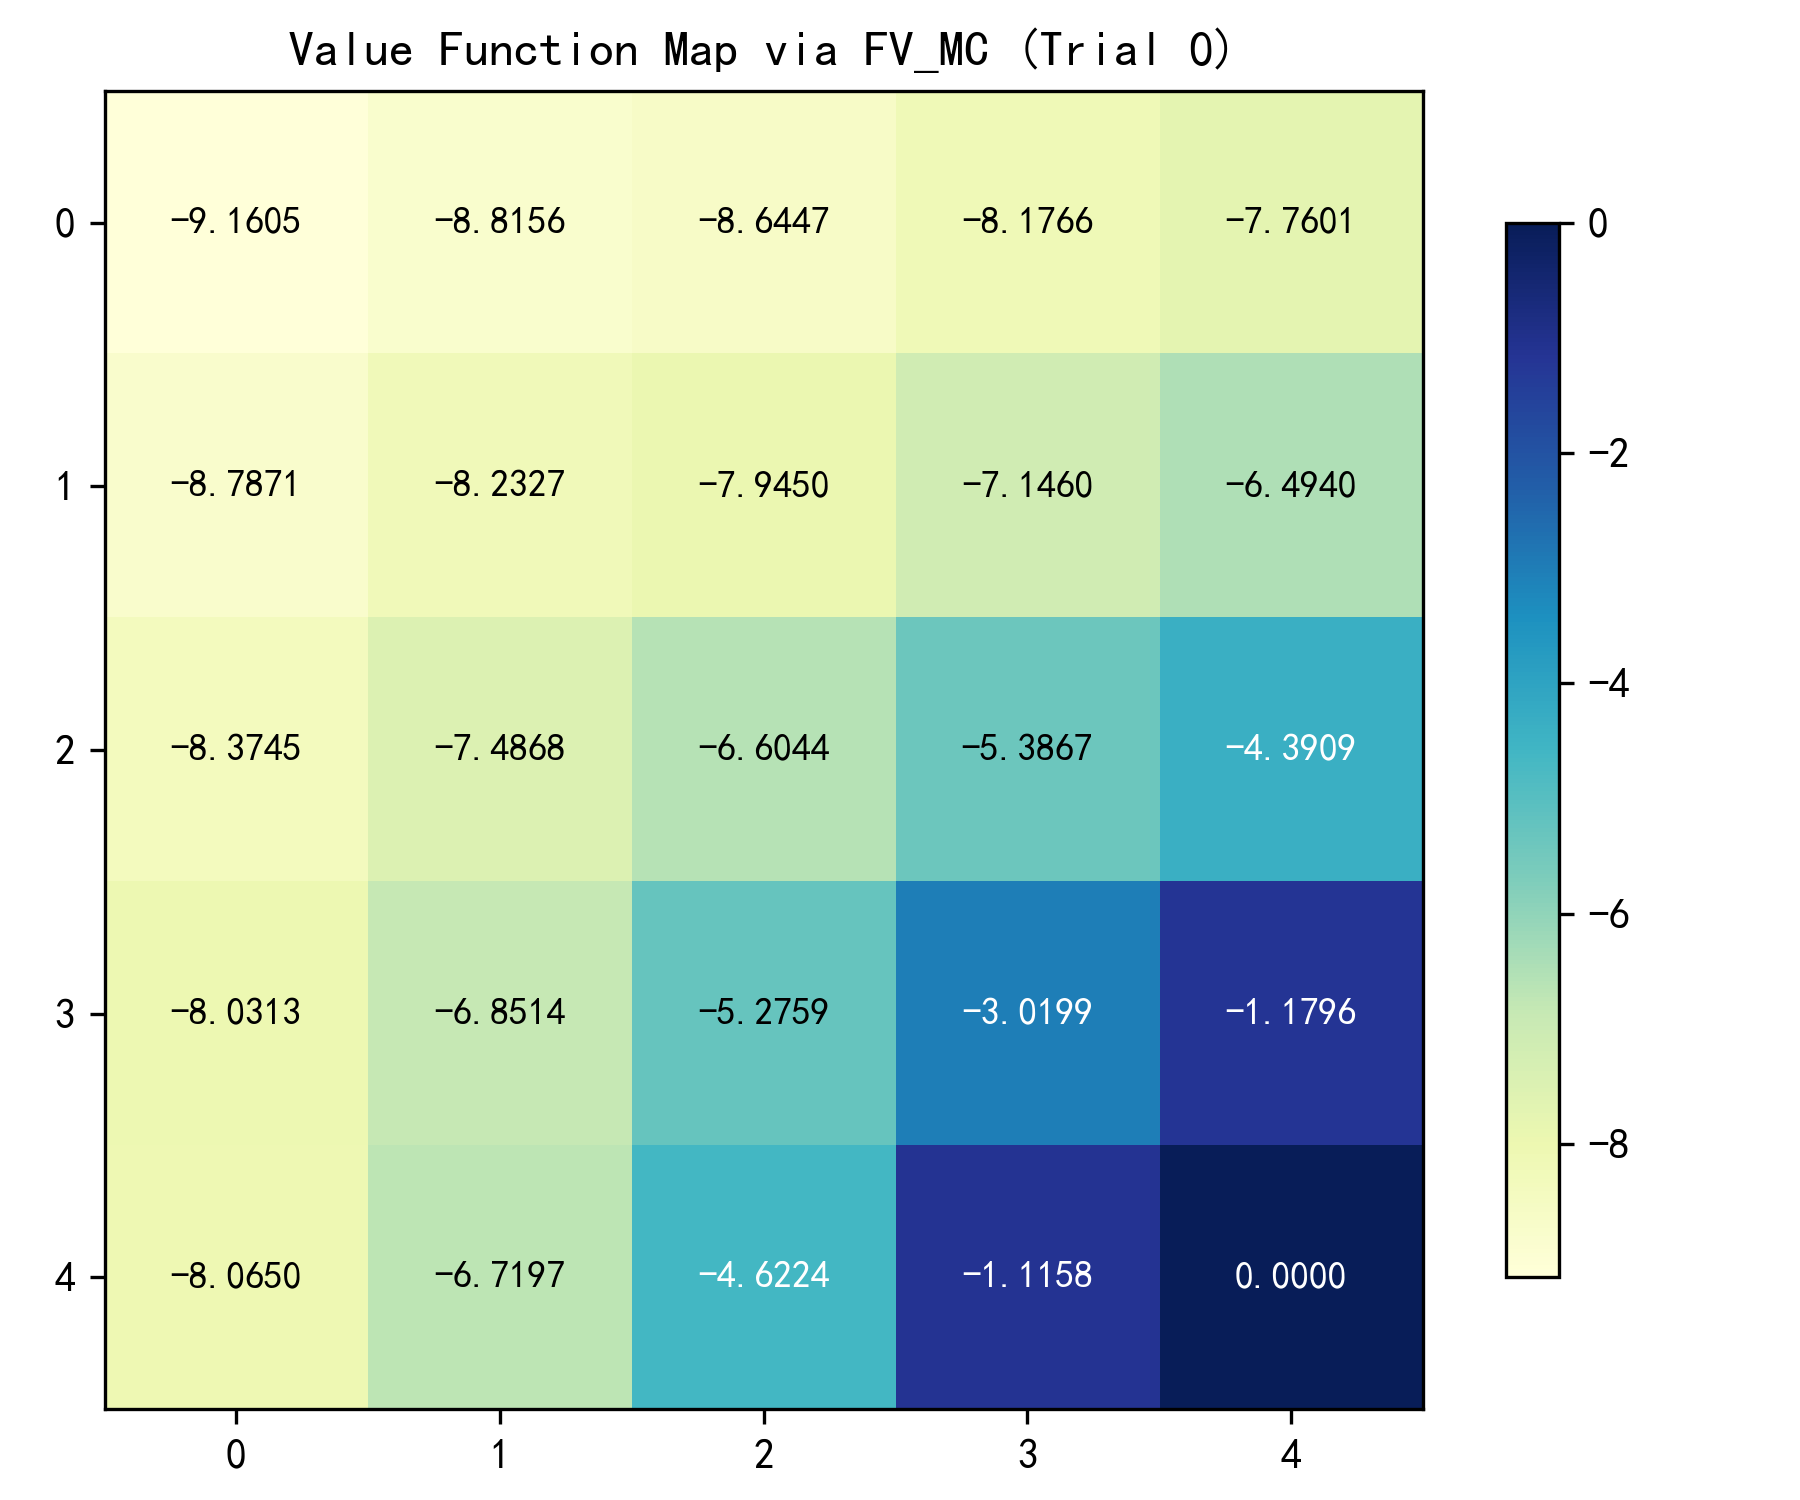
\includegraphics[width=\linewidth]{exp4/results/heatmap_FV_MC.png}
\end{minipage}
\caption{不同参数与方法下的估计状态价值热力图对比}
\end{figure}

\paragraph{结果分析}
\begin{enumerate}
\item \textbf{固定步长 TD(0)}：$\alpha=0.1$ 在前 100 个 episode 内下降更快，但收敛后的 RMSE 波动大于 $\alpha=0.05$。固定步长持续保留对新样本的响应，因此估计值会在真值附近波动；较大的步长带来更快的前期更新，也放大了稳态波动。
\item \textbf{访问次数衰减步长 TD(0)}：$\alpha_t=1/N(s_t)$ 随访问次数减小，曲线后期波动逐渐减弱。其前期估计受少量样本影响较大，后期更新幅度又较小，因此在本实验的 500 个 episode 内收敛较慢。
\item \textbf{FV-MC 与 TD(0)}：FV-MC 必须等待 episode 结束，并使用包含整条轨迹随机性的回报 $G_t$ 更新；TD(0) 每次转移后即可使用单步目标更新。图中 TD(0) 的 RMSE 下降更快且曲线更平滑，与两种更新目标的方差差异一致。
\end{enumerate}

\paragraph{思考题}


\question{问题 1：TD 与 MC 在是否 bootstrapping、是否等待完整 episode 结束方面有什么区别？}

\answerlabel TD 使用目标 $R_{t+1}+\gamma V(S_{t+1})$，其中包含下一状态的当前价值估计，因此属于自举更新。获得一次状态转移后即可计算该目标，不需要等待 episode 结束。

MC 使用完整回报
\[
G_t=\sum_{k=t}^{T-1}\gamma^{k-t}R_{k+1},
\]
不依赖后续状态的价值估计，因此不进行自举；但只有 episode 结束后才能得到 $G_t$。由此，TD 可在线更新，MC 的更新目标通常偏差较小但方差较大。


\question{问题 2：若初始价值函数全部设为 0，TD 更新中的 bootstrapping 会带来哪些优点和潜在偏差？}

\answerlabel 自举只依赖单步奖励和下一状态估计，能够在每次转移后更新，避免等待完整回合，并减少长轨迹回报带来的方差。

其代价是前期更新会受到初始估计影响。本实验中非终止状态的真实价值均为负数，而初始值为 0，因此初期目标偏高；这一偏差会沿相邻状态传播。随着各状态被反复访问，新奖励信息逐渐替代初始估计，偏差才会减小。


\subsubsection{任务 3：Sarsa 与 n-step Sarsa 控制算法}

n-step Sarsa 是 1-step Sarsa 与 MC 的统一推广：TD 目标使用从当前时刻起 $n$ 步的累积奖励再加 $n$ 步后的自举估计 $\hat{q}$，$n=1$ 退化为普通 Sarsa。较大的 $n$ 值使高价值信息可一次性跨越 $n$ 步回传，显著加快前期收敛效率，以更大的方差为代价换取更小的偏差。

\paragraph{实验设置}
本任务在 GridWorld 中学习从固定起点 $(0,0)$ 到目标点 $(4,4)$ 的控制策略，对比 $n\in\{1,3,5\}$ 的 n-step Sarsa，其中 $n=1$ 为普通 Sarsa。统一设置 $\epsilon=0.1$、$\alpha=0.1$、$\gamma=0.9$，每个 episode 最多运行 200 步；实验使用 20 个独立随机种子，每个随机种子运行 500 个 episode。

\paragraph{学习曲线对比}
以下是累计奖励（Episode Reward）、到达目标步数（Steps to Goal）和成功率（Success Rate）随 episode 变化的对比图：

\begin{figure}[H]
\centering
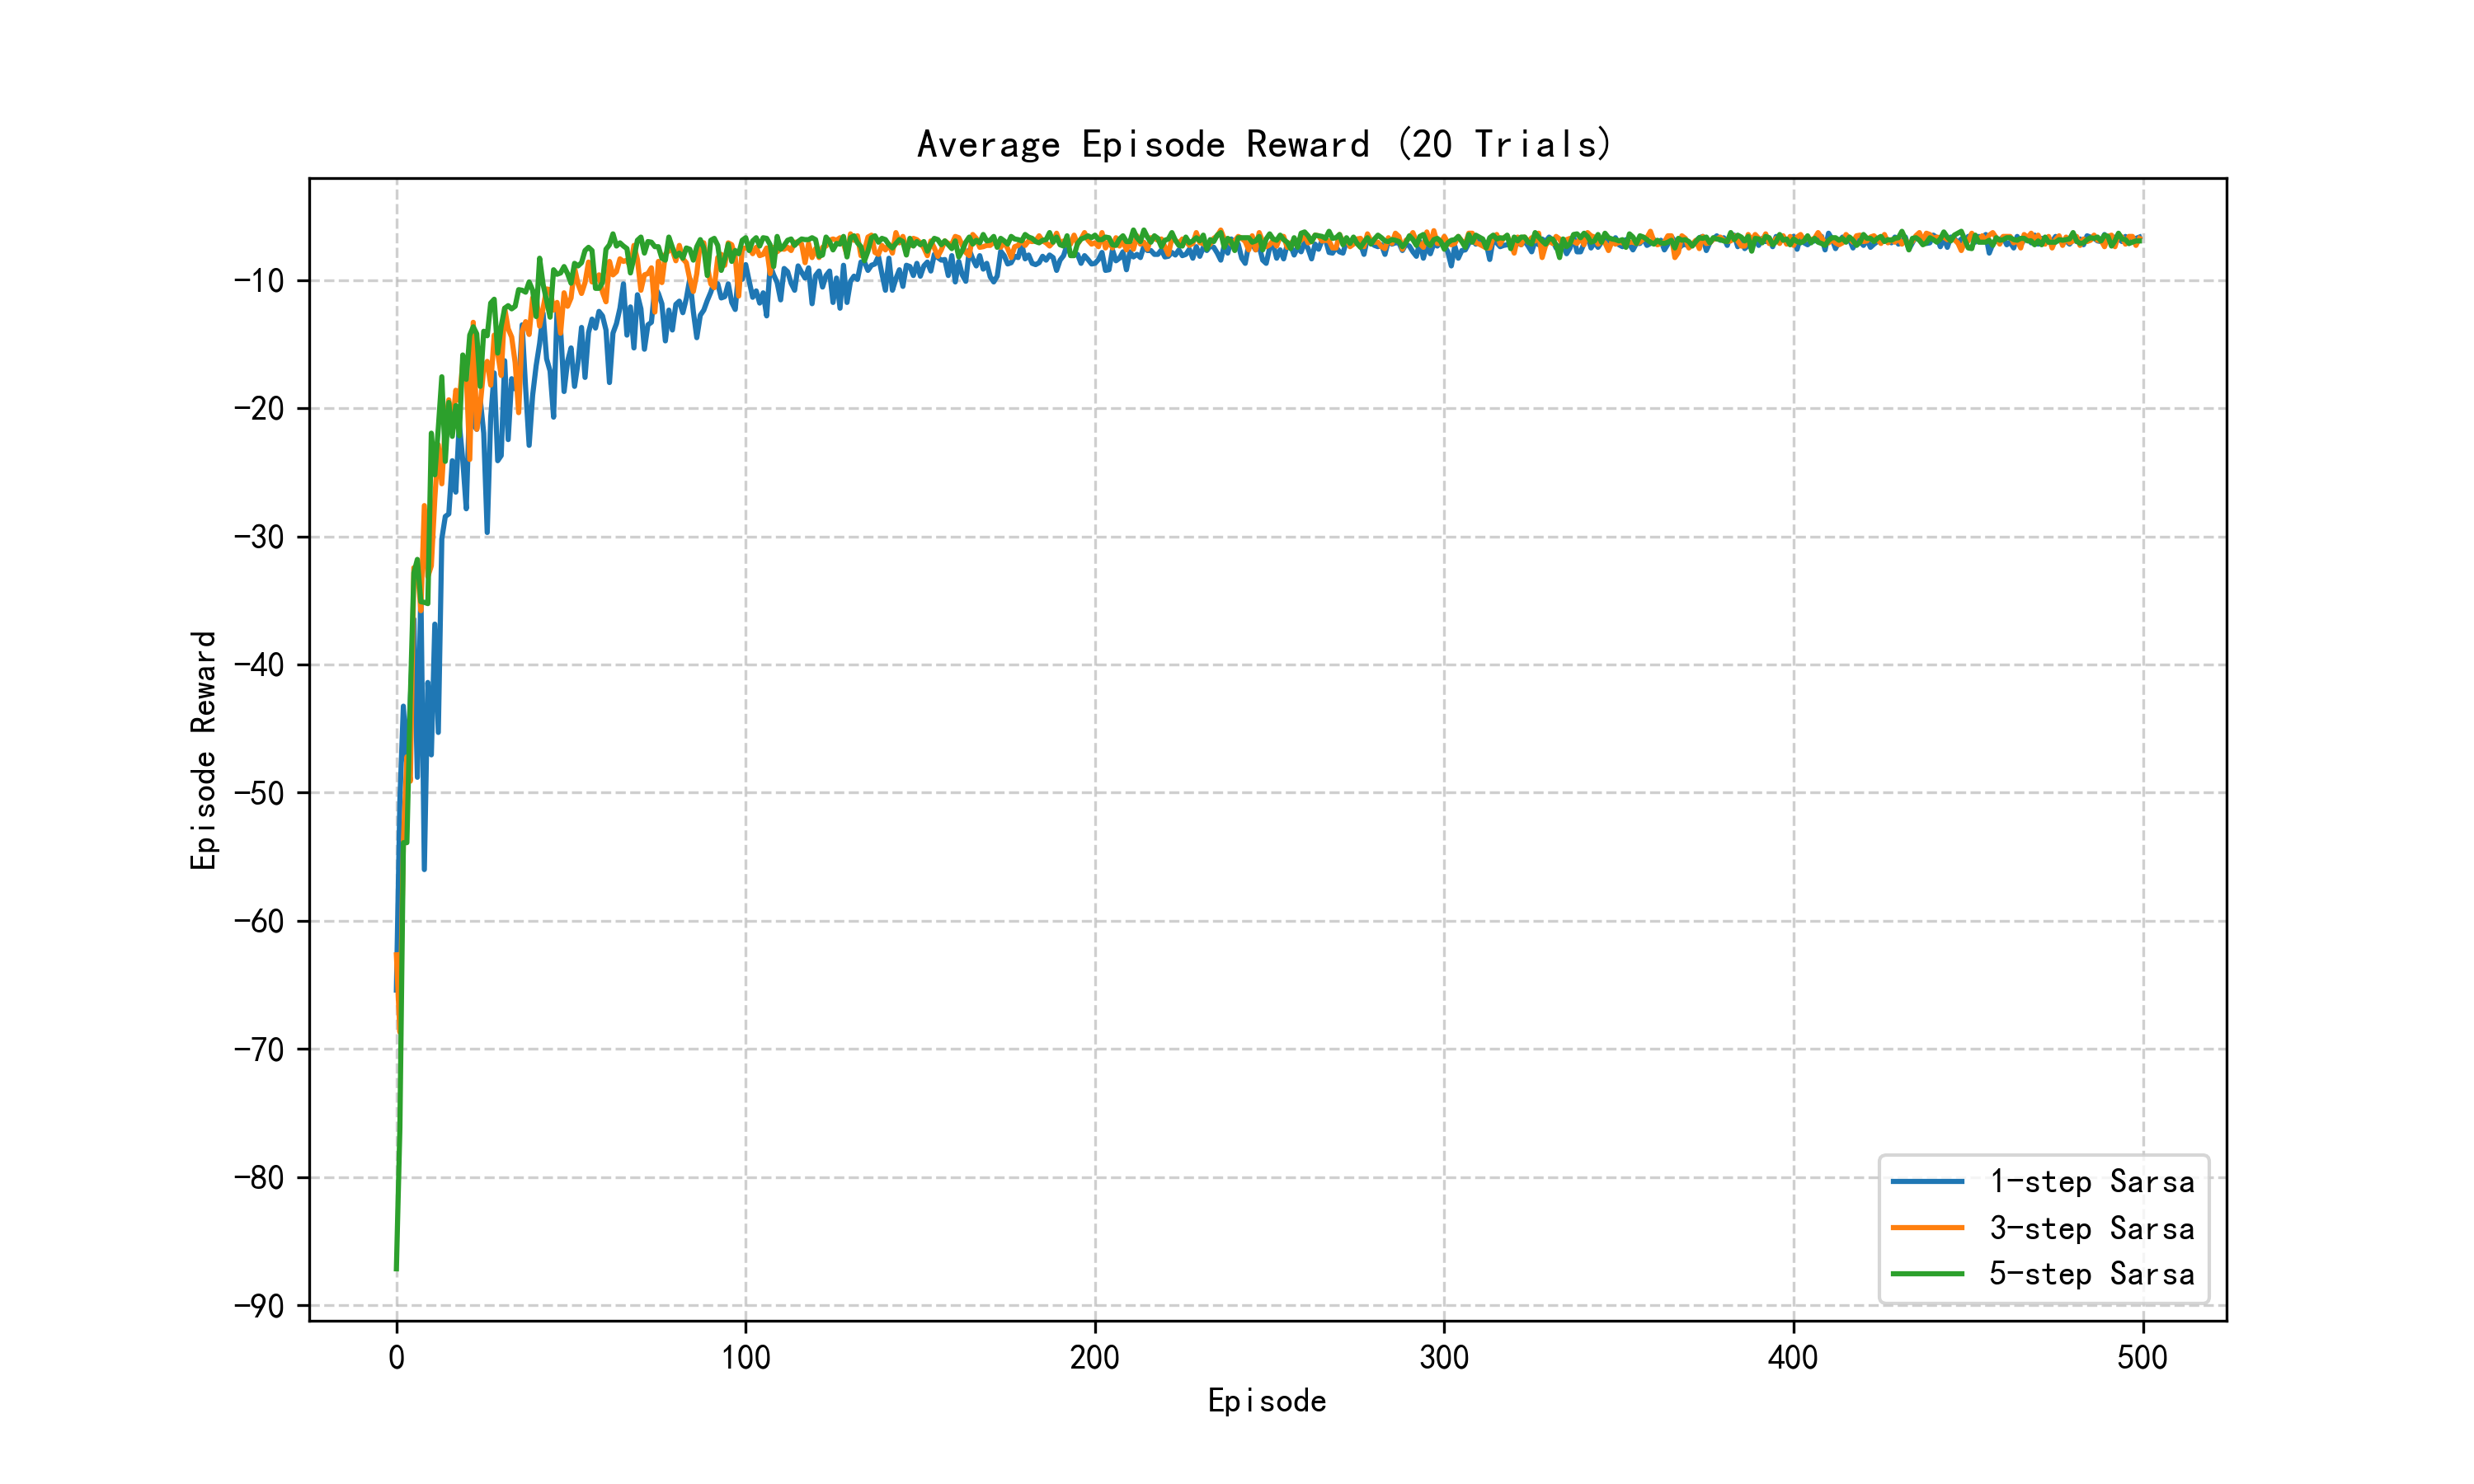
\includegraphics[width=0.7\textwidth]{exp4/results/task3_rewards.png}
\caption{Sarsa 与 n-step Sarsa 累计奖励曲线}
\end{figure}

\begin{figure}[H]
\centering
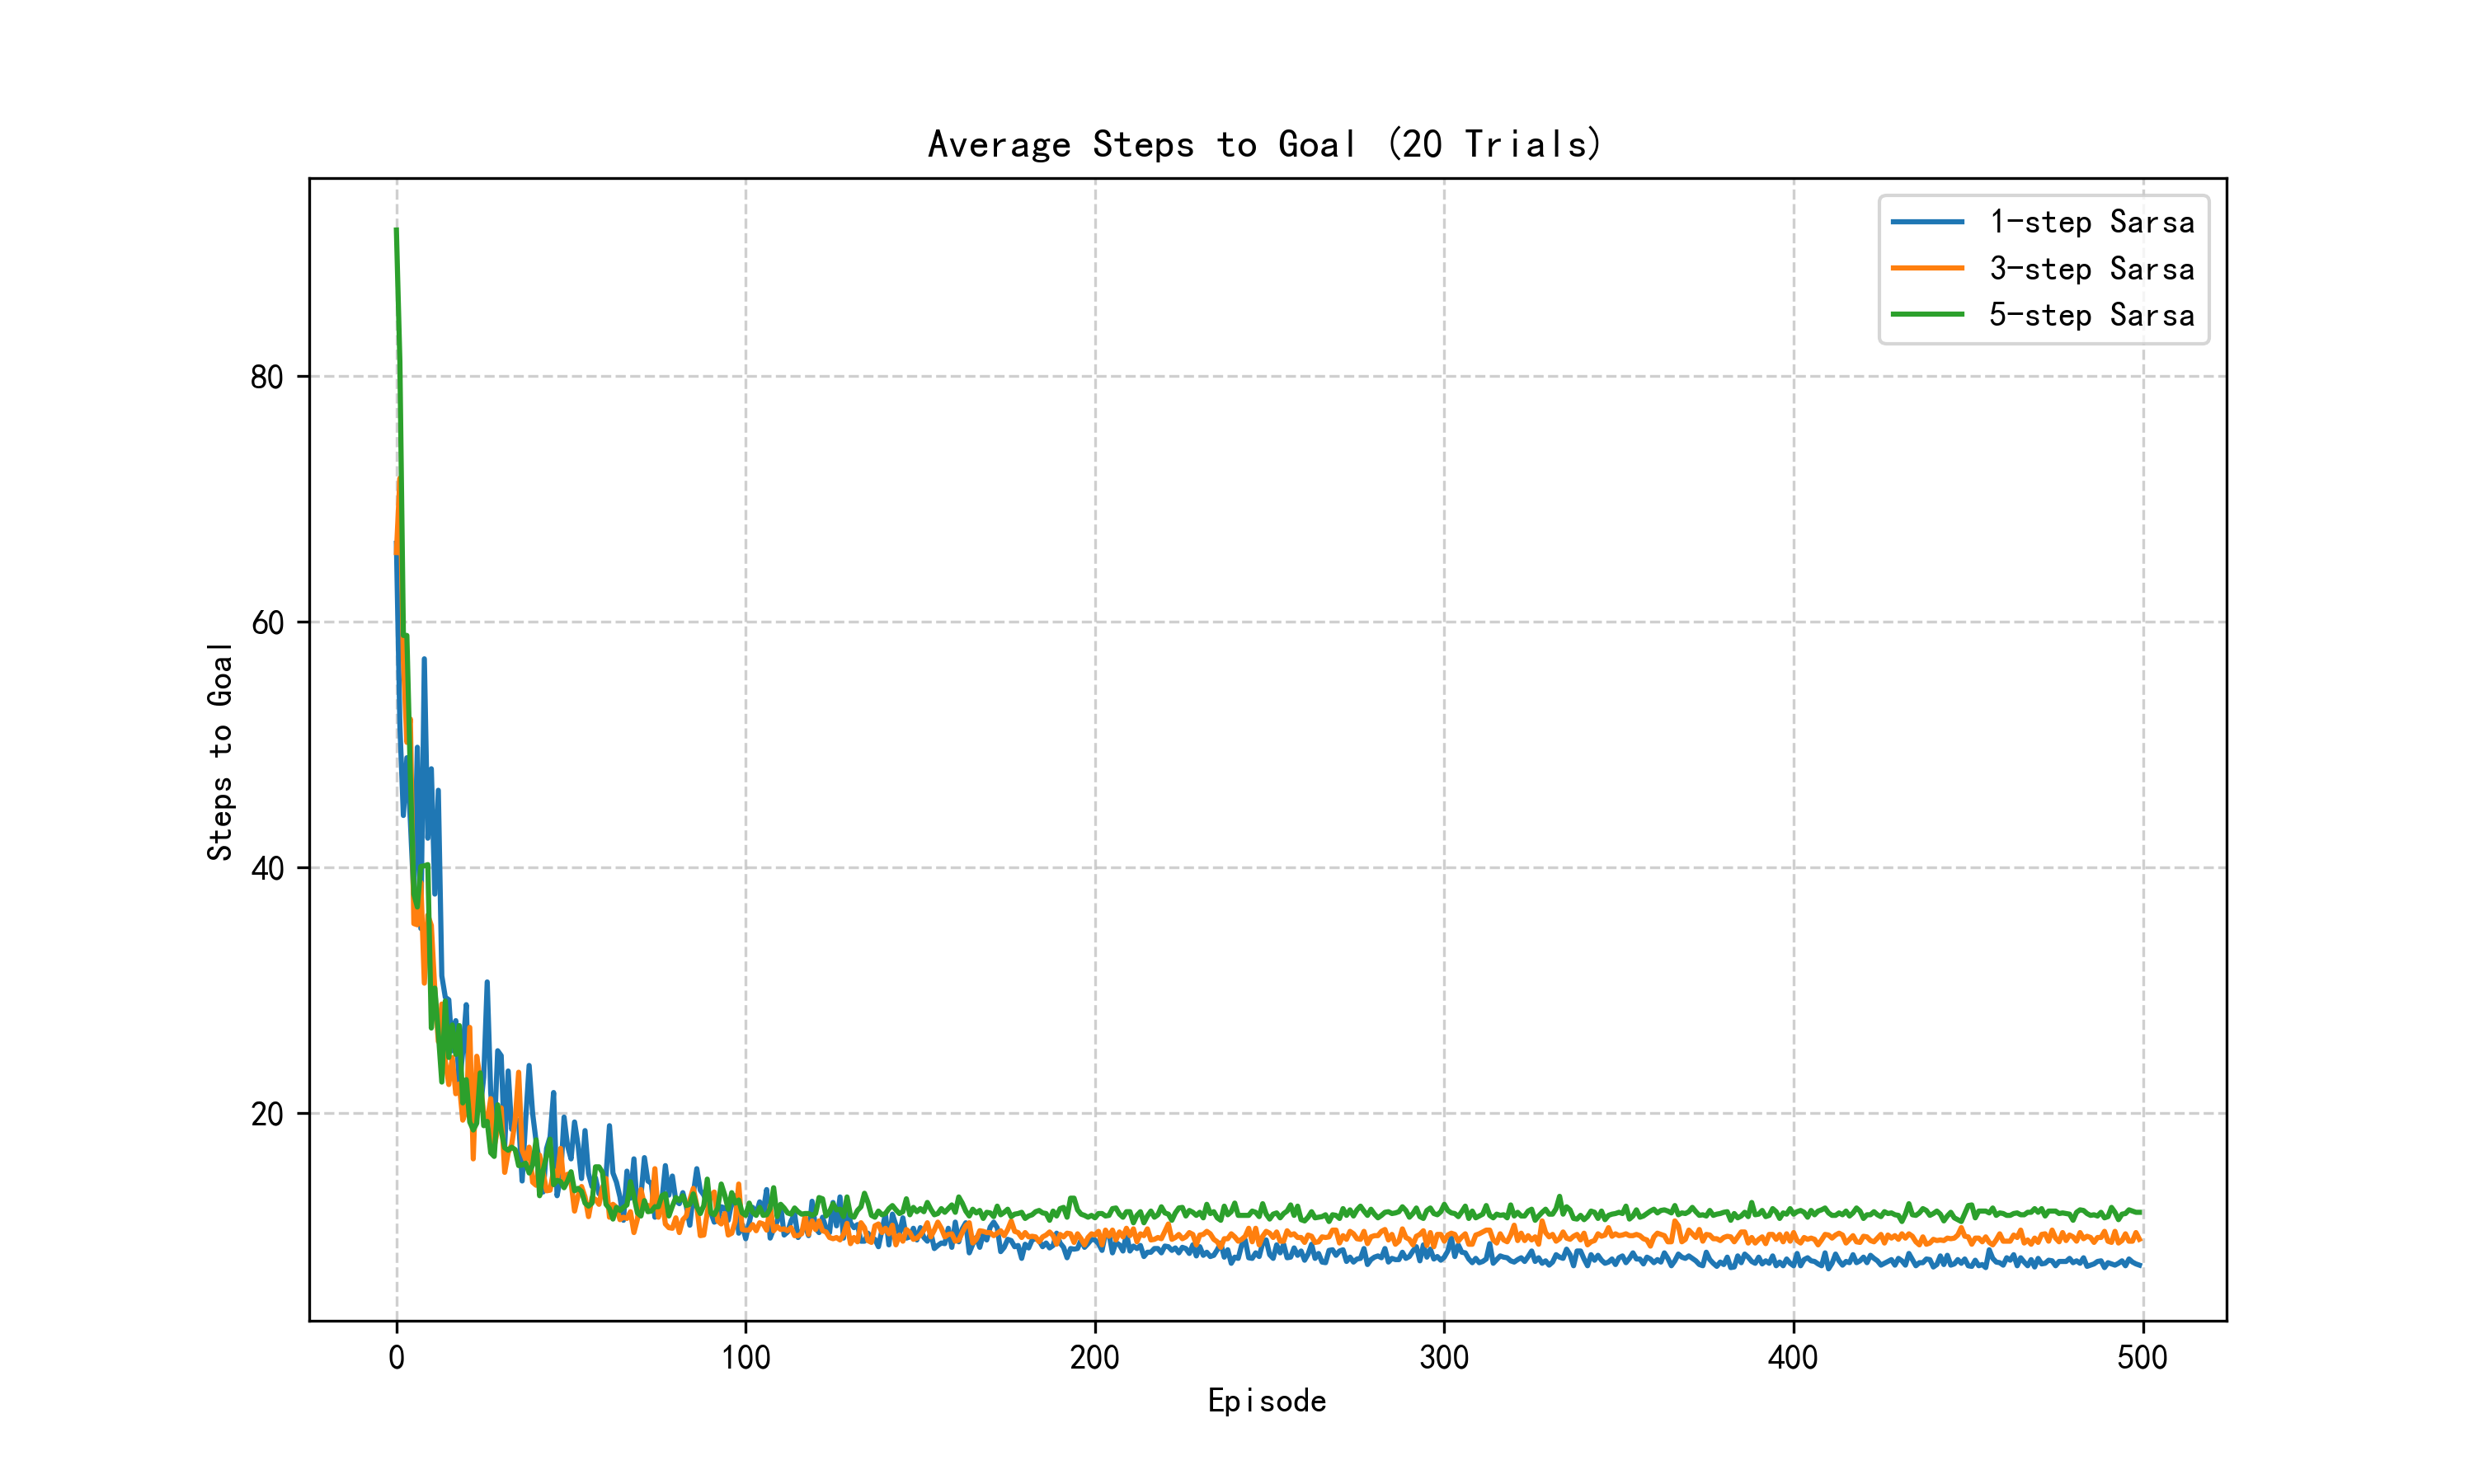
\includegraphics[width=0.7\textwidth]{exp4/results/task3_steps.png}
\caption{Sarsa 与 n-step Sarsa 到达目标步数曲线}
\end{figure}

\begin{figure}[H]
\centering
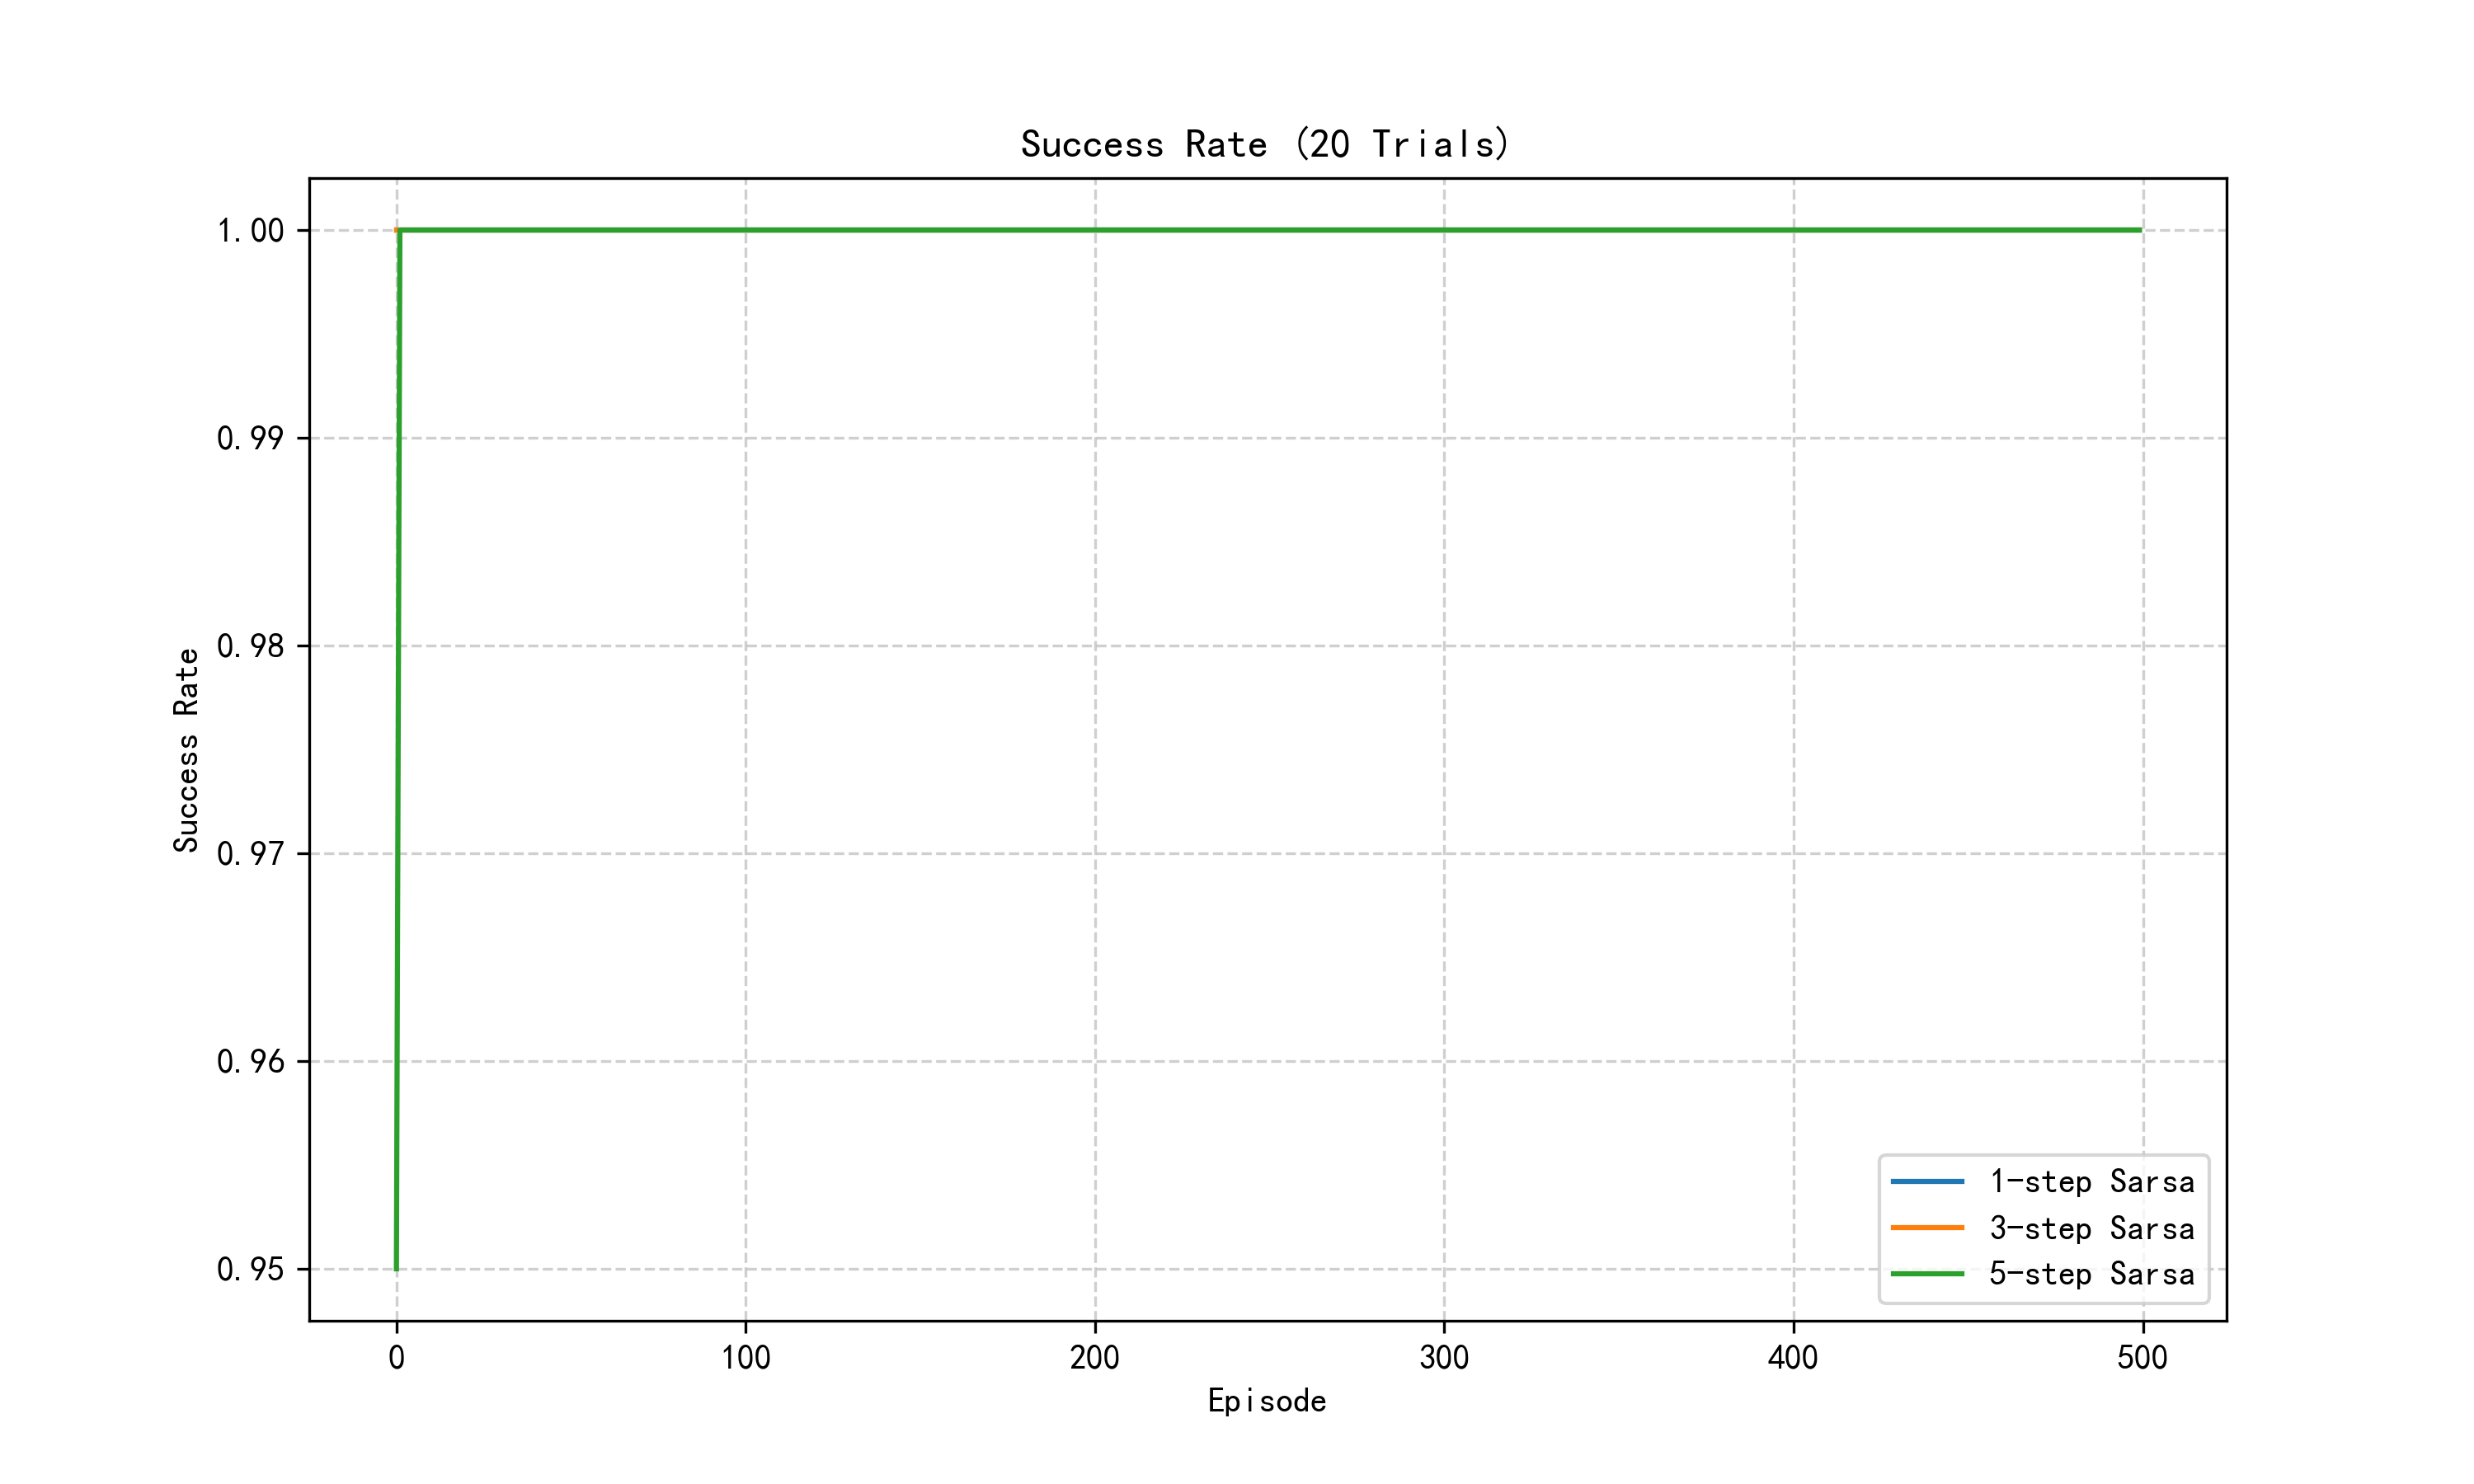
\includegraphics[width=0.7\textwidth]{exp4/results/task3_success_rate.png}
\caption{Sarsa 与 n-step Sarsa 成功率收敛曲线}
\end{figure}

\paragraph{最终贪心策略箭头图}
以下是 Trial 0 结束后，不同 $n$ 值下学到的贪心策略箭头图（指向 $Q$ 值最大的动作，G 为目标）：

\begin{figure}[H]
\centering
\begin{minipage}{0.32\textwidth}
\centering
\textbf{Sarsa ($n=1$)}\\[0.4em]
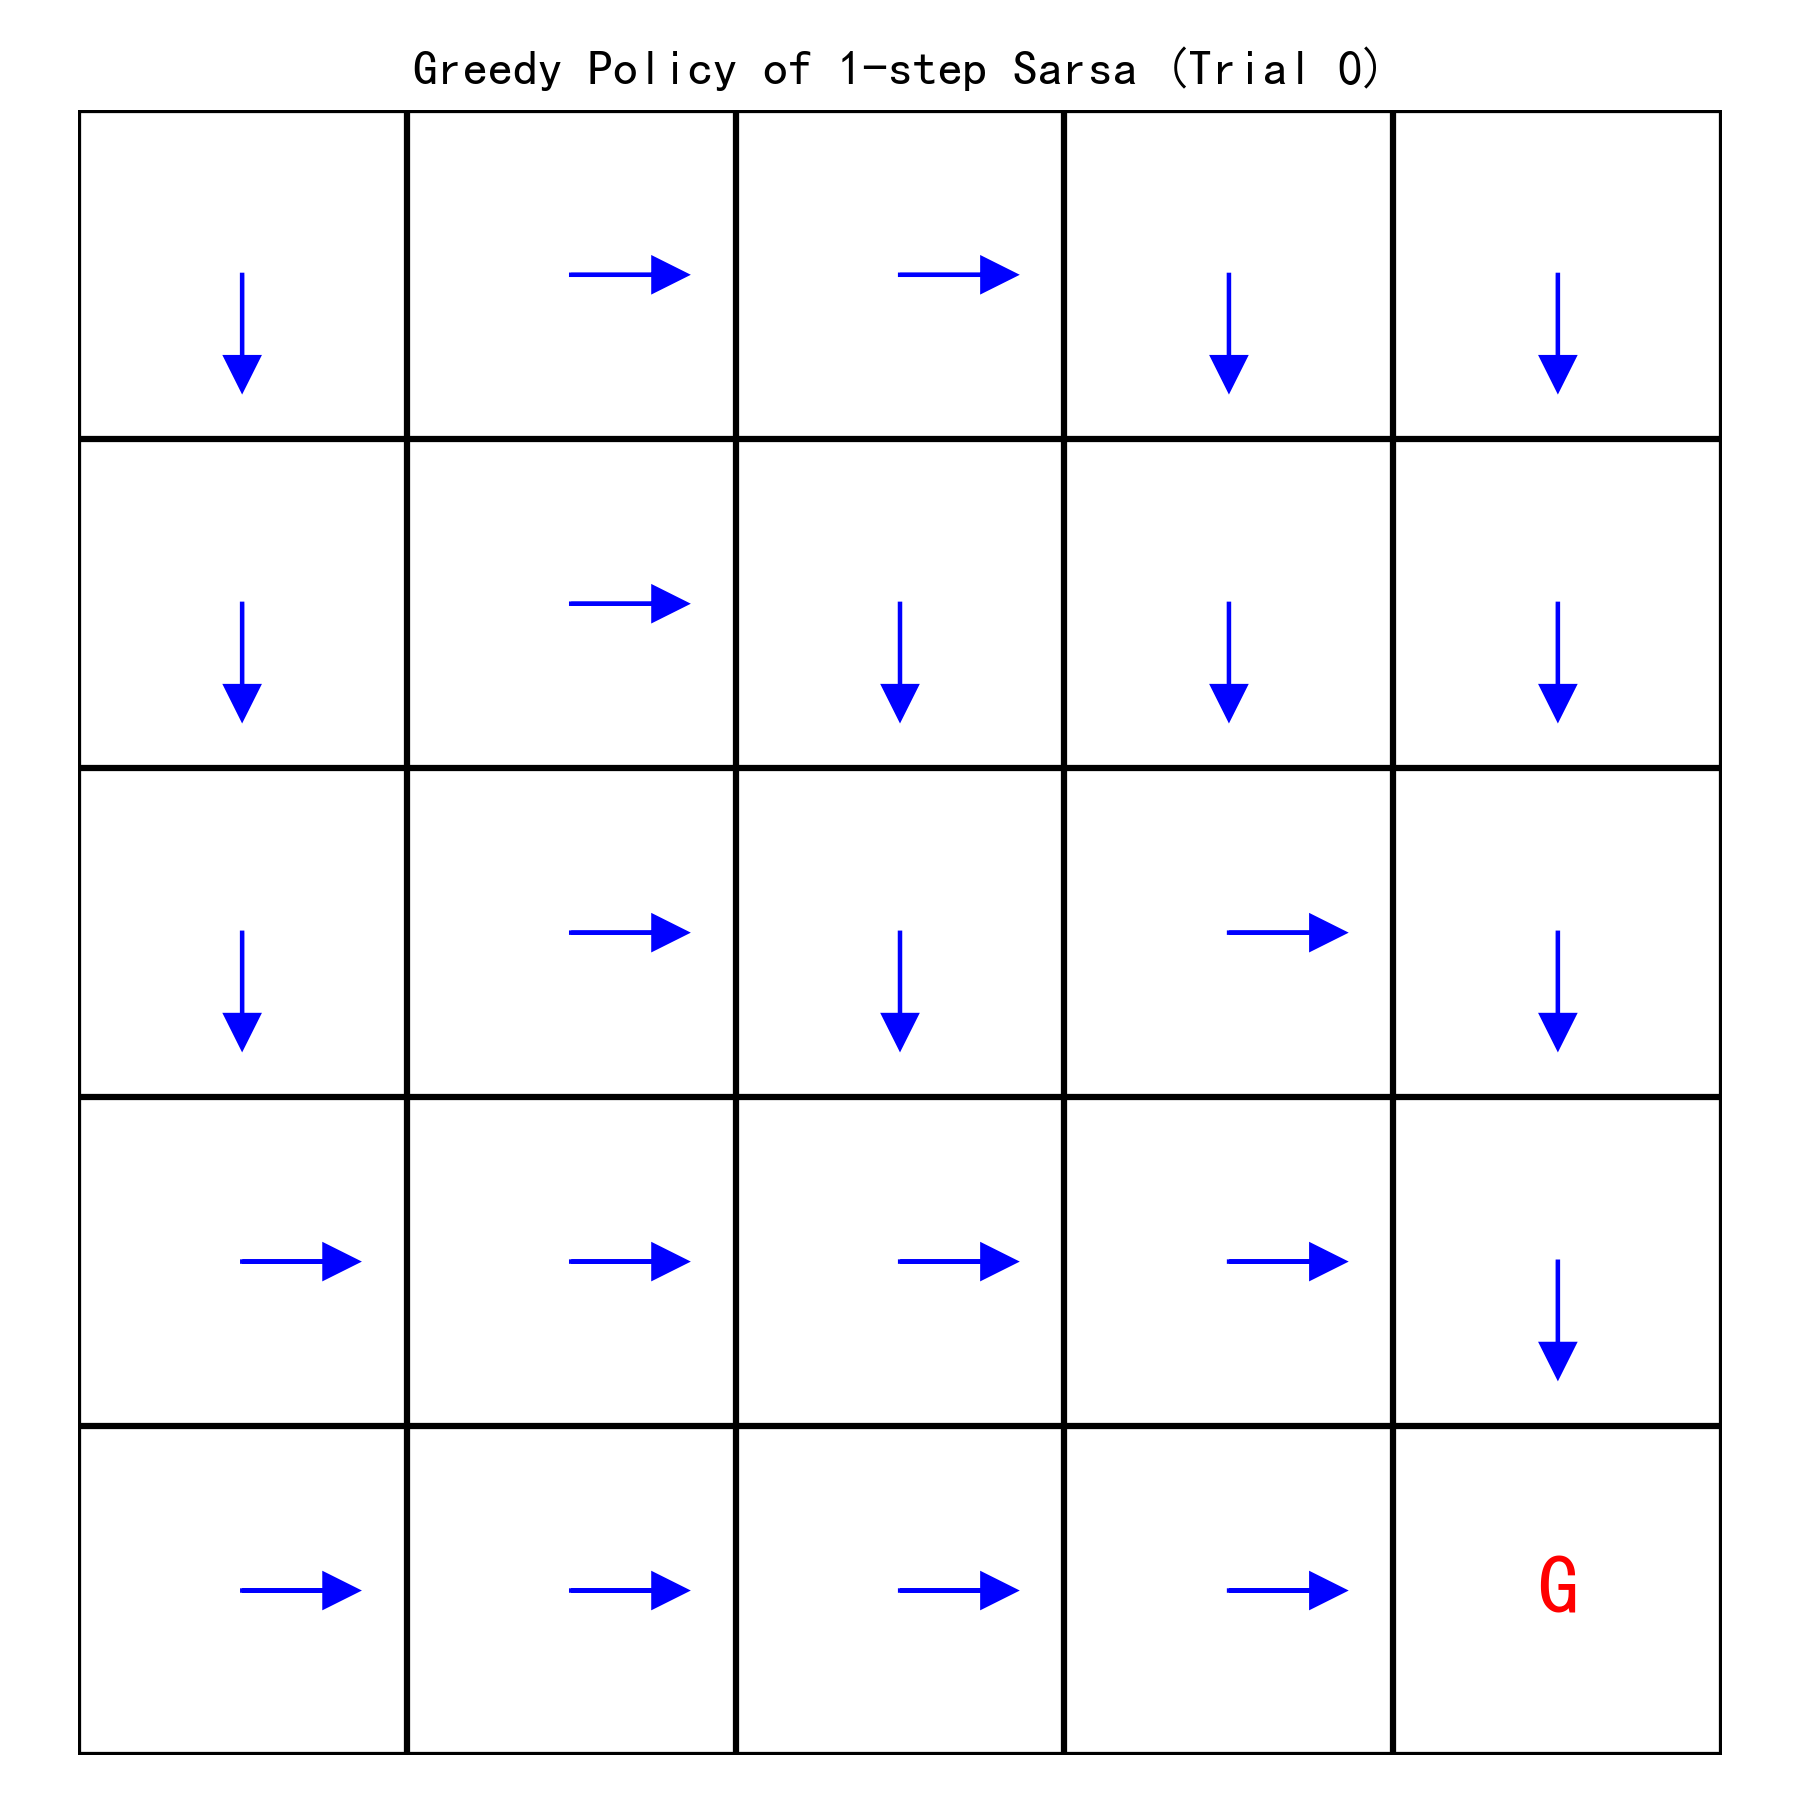
\includegraphics[width=\linewidth]{exp4/results/task3_policy_n1.png}
\end{minipage}\hfill
\begin{minipage}{0.32\textwidth}
\centering
\textbf{n-step Sarsa ($n=3$)}\\[0.4em]
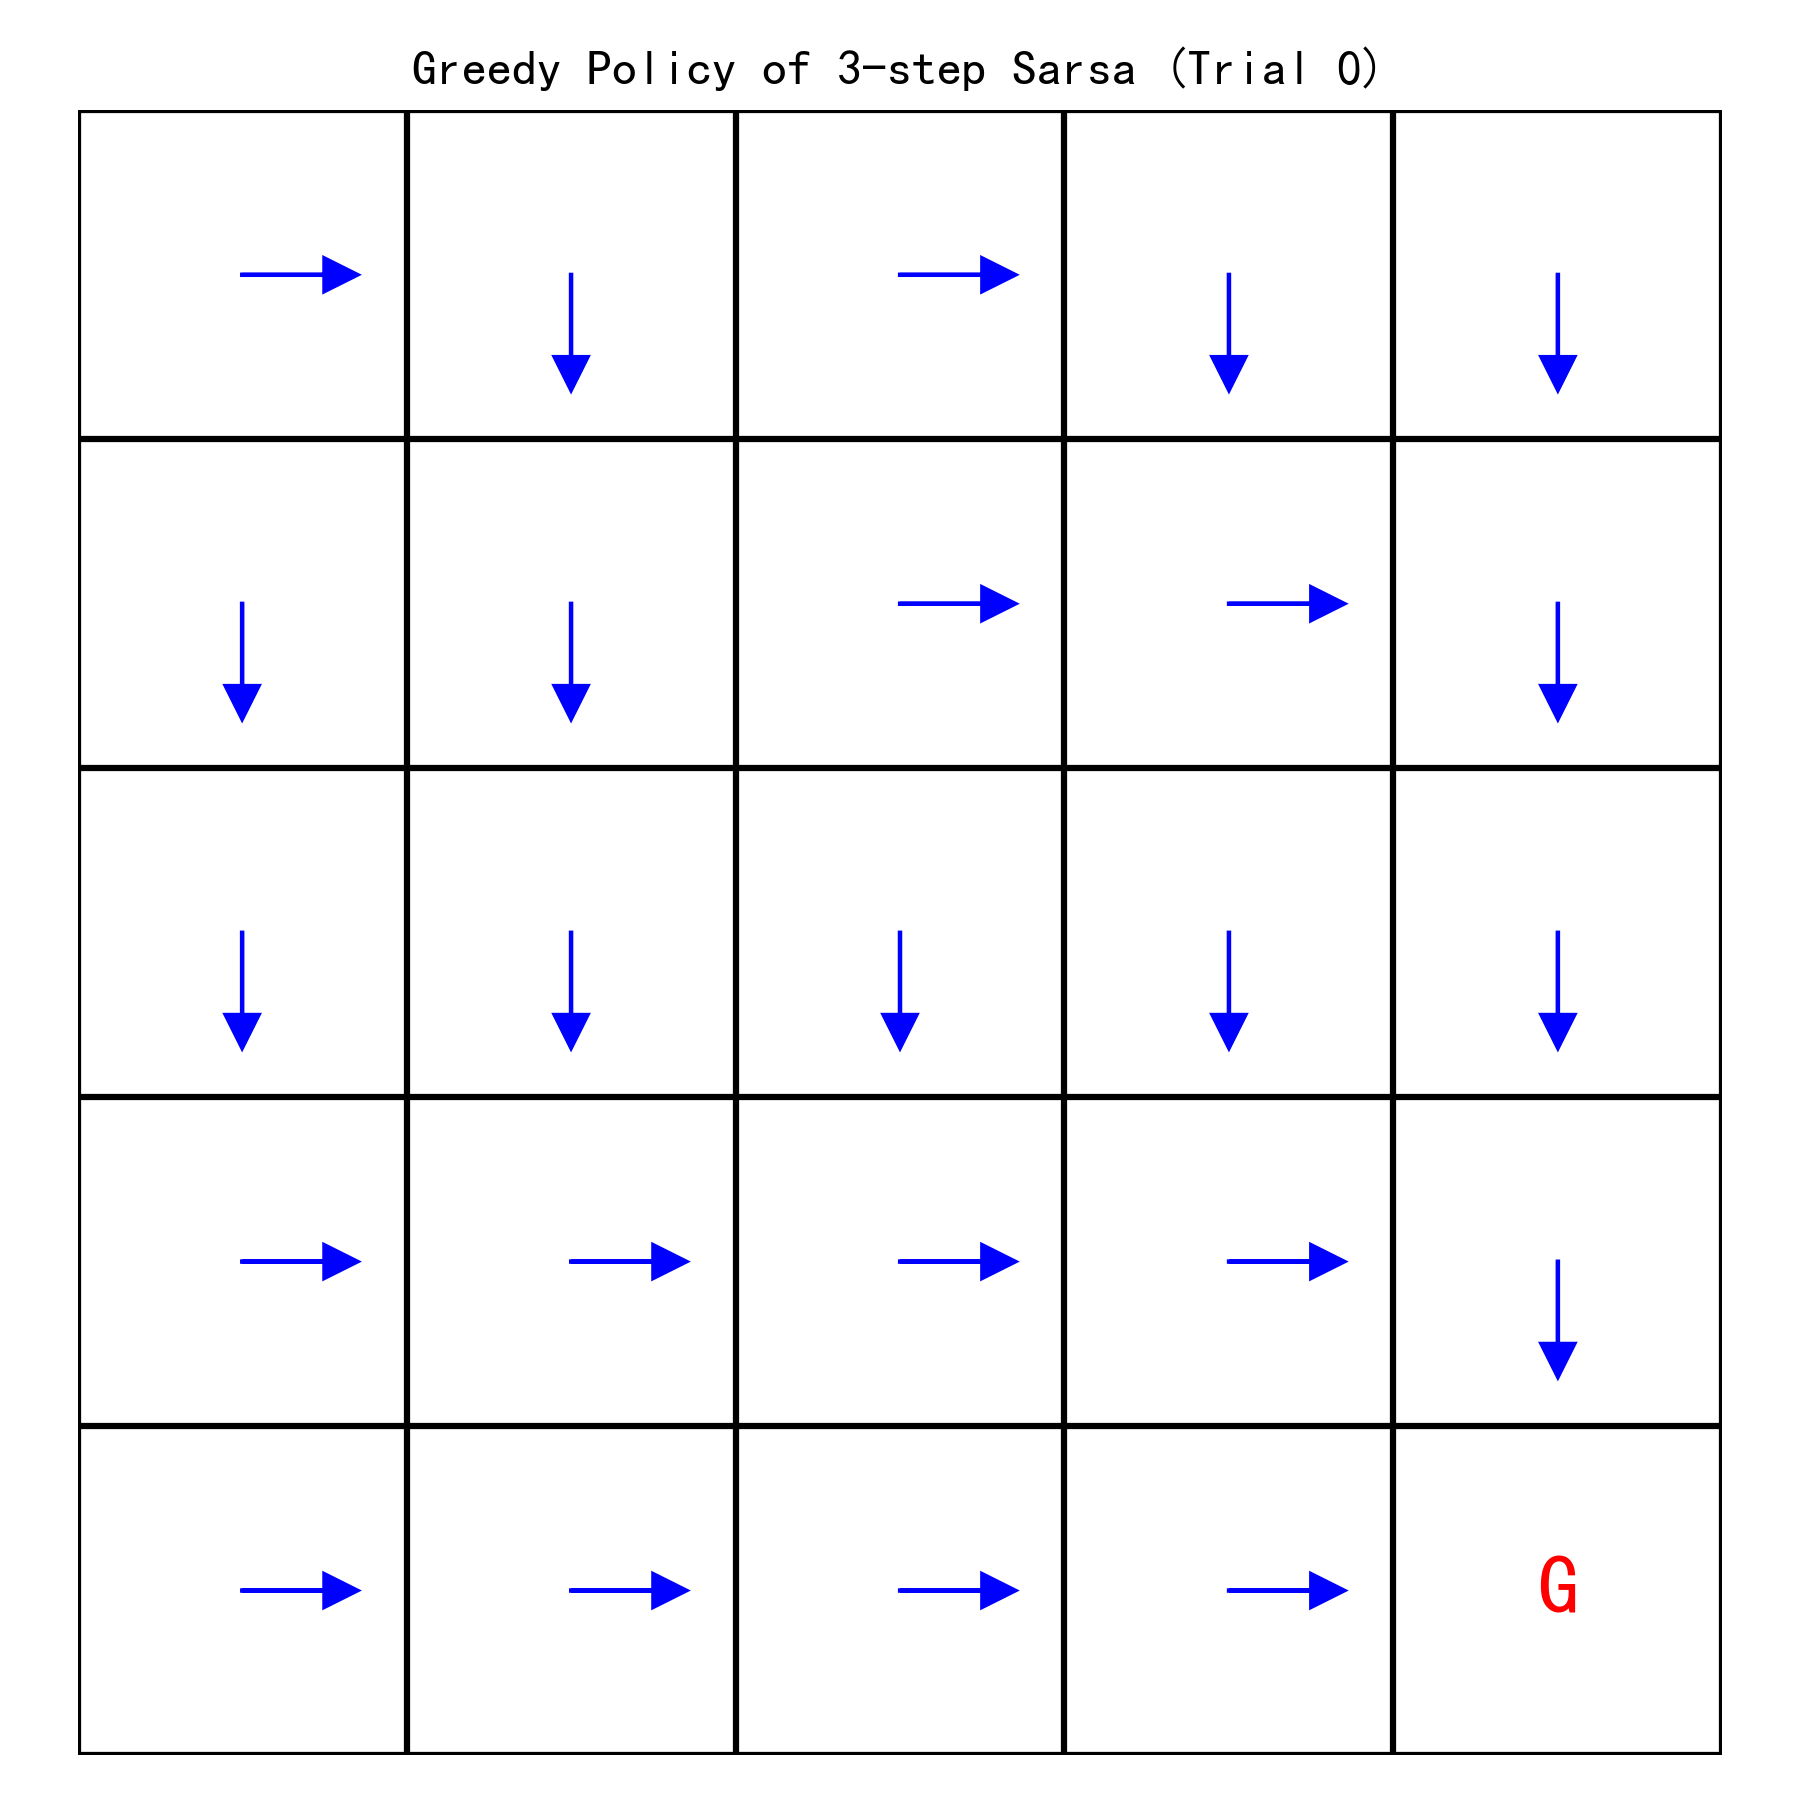
\includegraphics[width=\linewidth]{exp4/results/task3_policy_n3.png}
\end{minipage}\hfill
\begin{minipage}{0.32\textwidth}
\centering
\textbf{n-step Sarsa ($n=5$)}\\[0.4em]
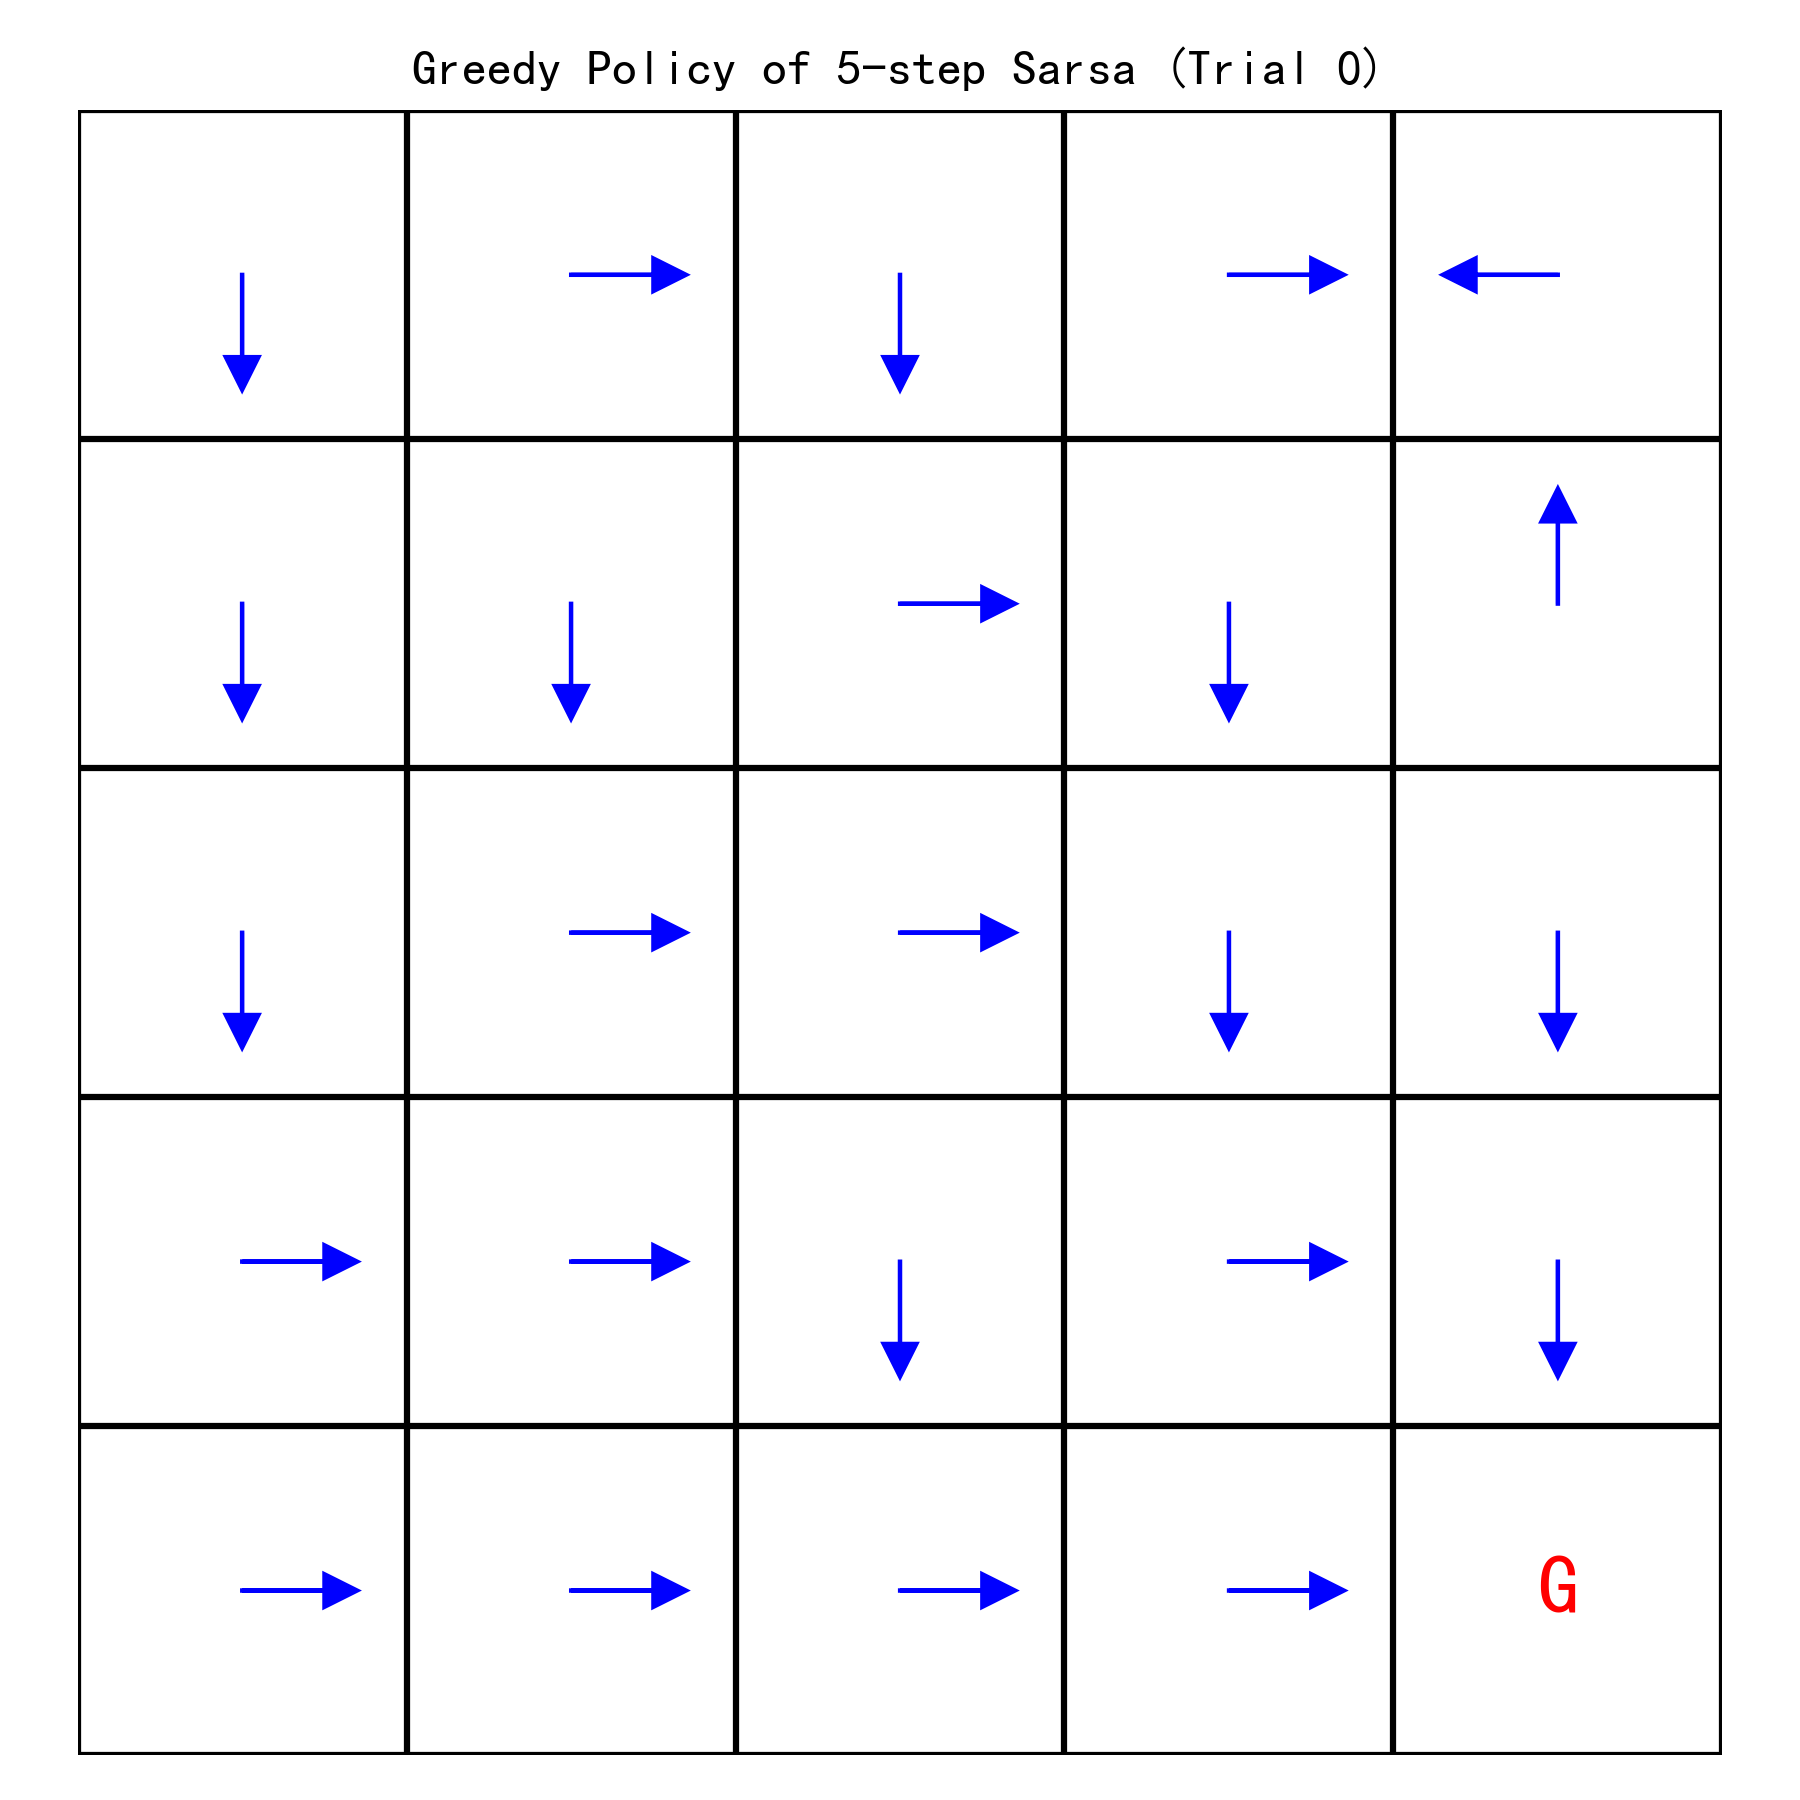
\includegraphics[width=\linewidth]{exp4/results/task3_policy_n5.png}
\end{minipage}
\caption{不同 $n$ 值下的最终贪心策略}
\end{figure}

\paragraph{结果分析}
\begin{enumerate}
\item \textbf{收敛速度}：$n=3$ 和 $n=5$ 在约 20--40 个 episode 后进入稳定区间，$n=1$ 约在第 80 个 episode 后达到相近成功率。多步目标能够在一次更新中向前传播更多奖励信息，因此前期学习更快。
\item \textbf{最终性能}：三个配置最终均达到 100\% 成功率，并从起点形成 8 步最短路径。按照本环境的奖励规则，7 次普通移动和最后一次到达目标对应累计奖励 $-6$。
\item \textbf{适用边界}：本实验只比较了确定性小规模 GridWorld 中的三个 $n$ 值。增大 $n$ 会引入更多未来奖励和动作选择的随机性，因此不能据此断言更大的 $n$ 在其他环境中一定更快。
\end{enumerate}

\paragraph{思考题}



\question{问题：$n$ 从 1 增大时，更新目标更接近 TD 还是 Monte Carlo？这对偏差和方差有什么影响？}

\answerlabel $n$-step 目标为
\[
G_t^{(n)}=\sum_{k=1}^{n}\gamma^{k-1}R_{t+k}
          +\gamma^n Q(S_{t+n},A_{t+n}).
\]
随着 $n$ 增大，目标中实际观测奖励所占比例增加，自举项的影响减小，因此更新逐渐接近 Monte Carlo；当 $n$ 覆盖至 episode 终点时，自举项消失。

减少自举通常会降低由当前价值估计引入的偏差，但纳入更多随机转移和探索动作会提高目标方差。因此 $n$ 控制的是偏差与方差之间的折中。本实验中 $n=3$ 和 $n=5$ 前期收敛较快，但这一结果依赖当前环境和参数。


\subsubsection{任务 4：Q-learning 与 Sarsa 在线控制对比}

\paragraph{实验设置}
本任务在同一 GridWorld 中在线比较 Sarsa 与 Q-learning。两种算法均使用 $\epsilon$-greedy 行为策略生成交互数据，并采用相同的随机种子和超参数。区别仅在 TD 目标：Sarsa 使用行为策略实际选择的下一动作，Q-learning 使用下一状态中的最大动作价值。

\paragraph{学习曲线与最终策略}
下列曲线为 20 次独立运行的平均结果，最终策略图取自 Trial 0。

\begin{figure}[H]
\centering
\begin{minipage}{0.49\textwidth}
\centering
\textbf{累计奖励}\\[0.4em]
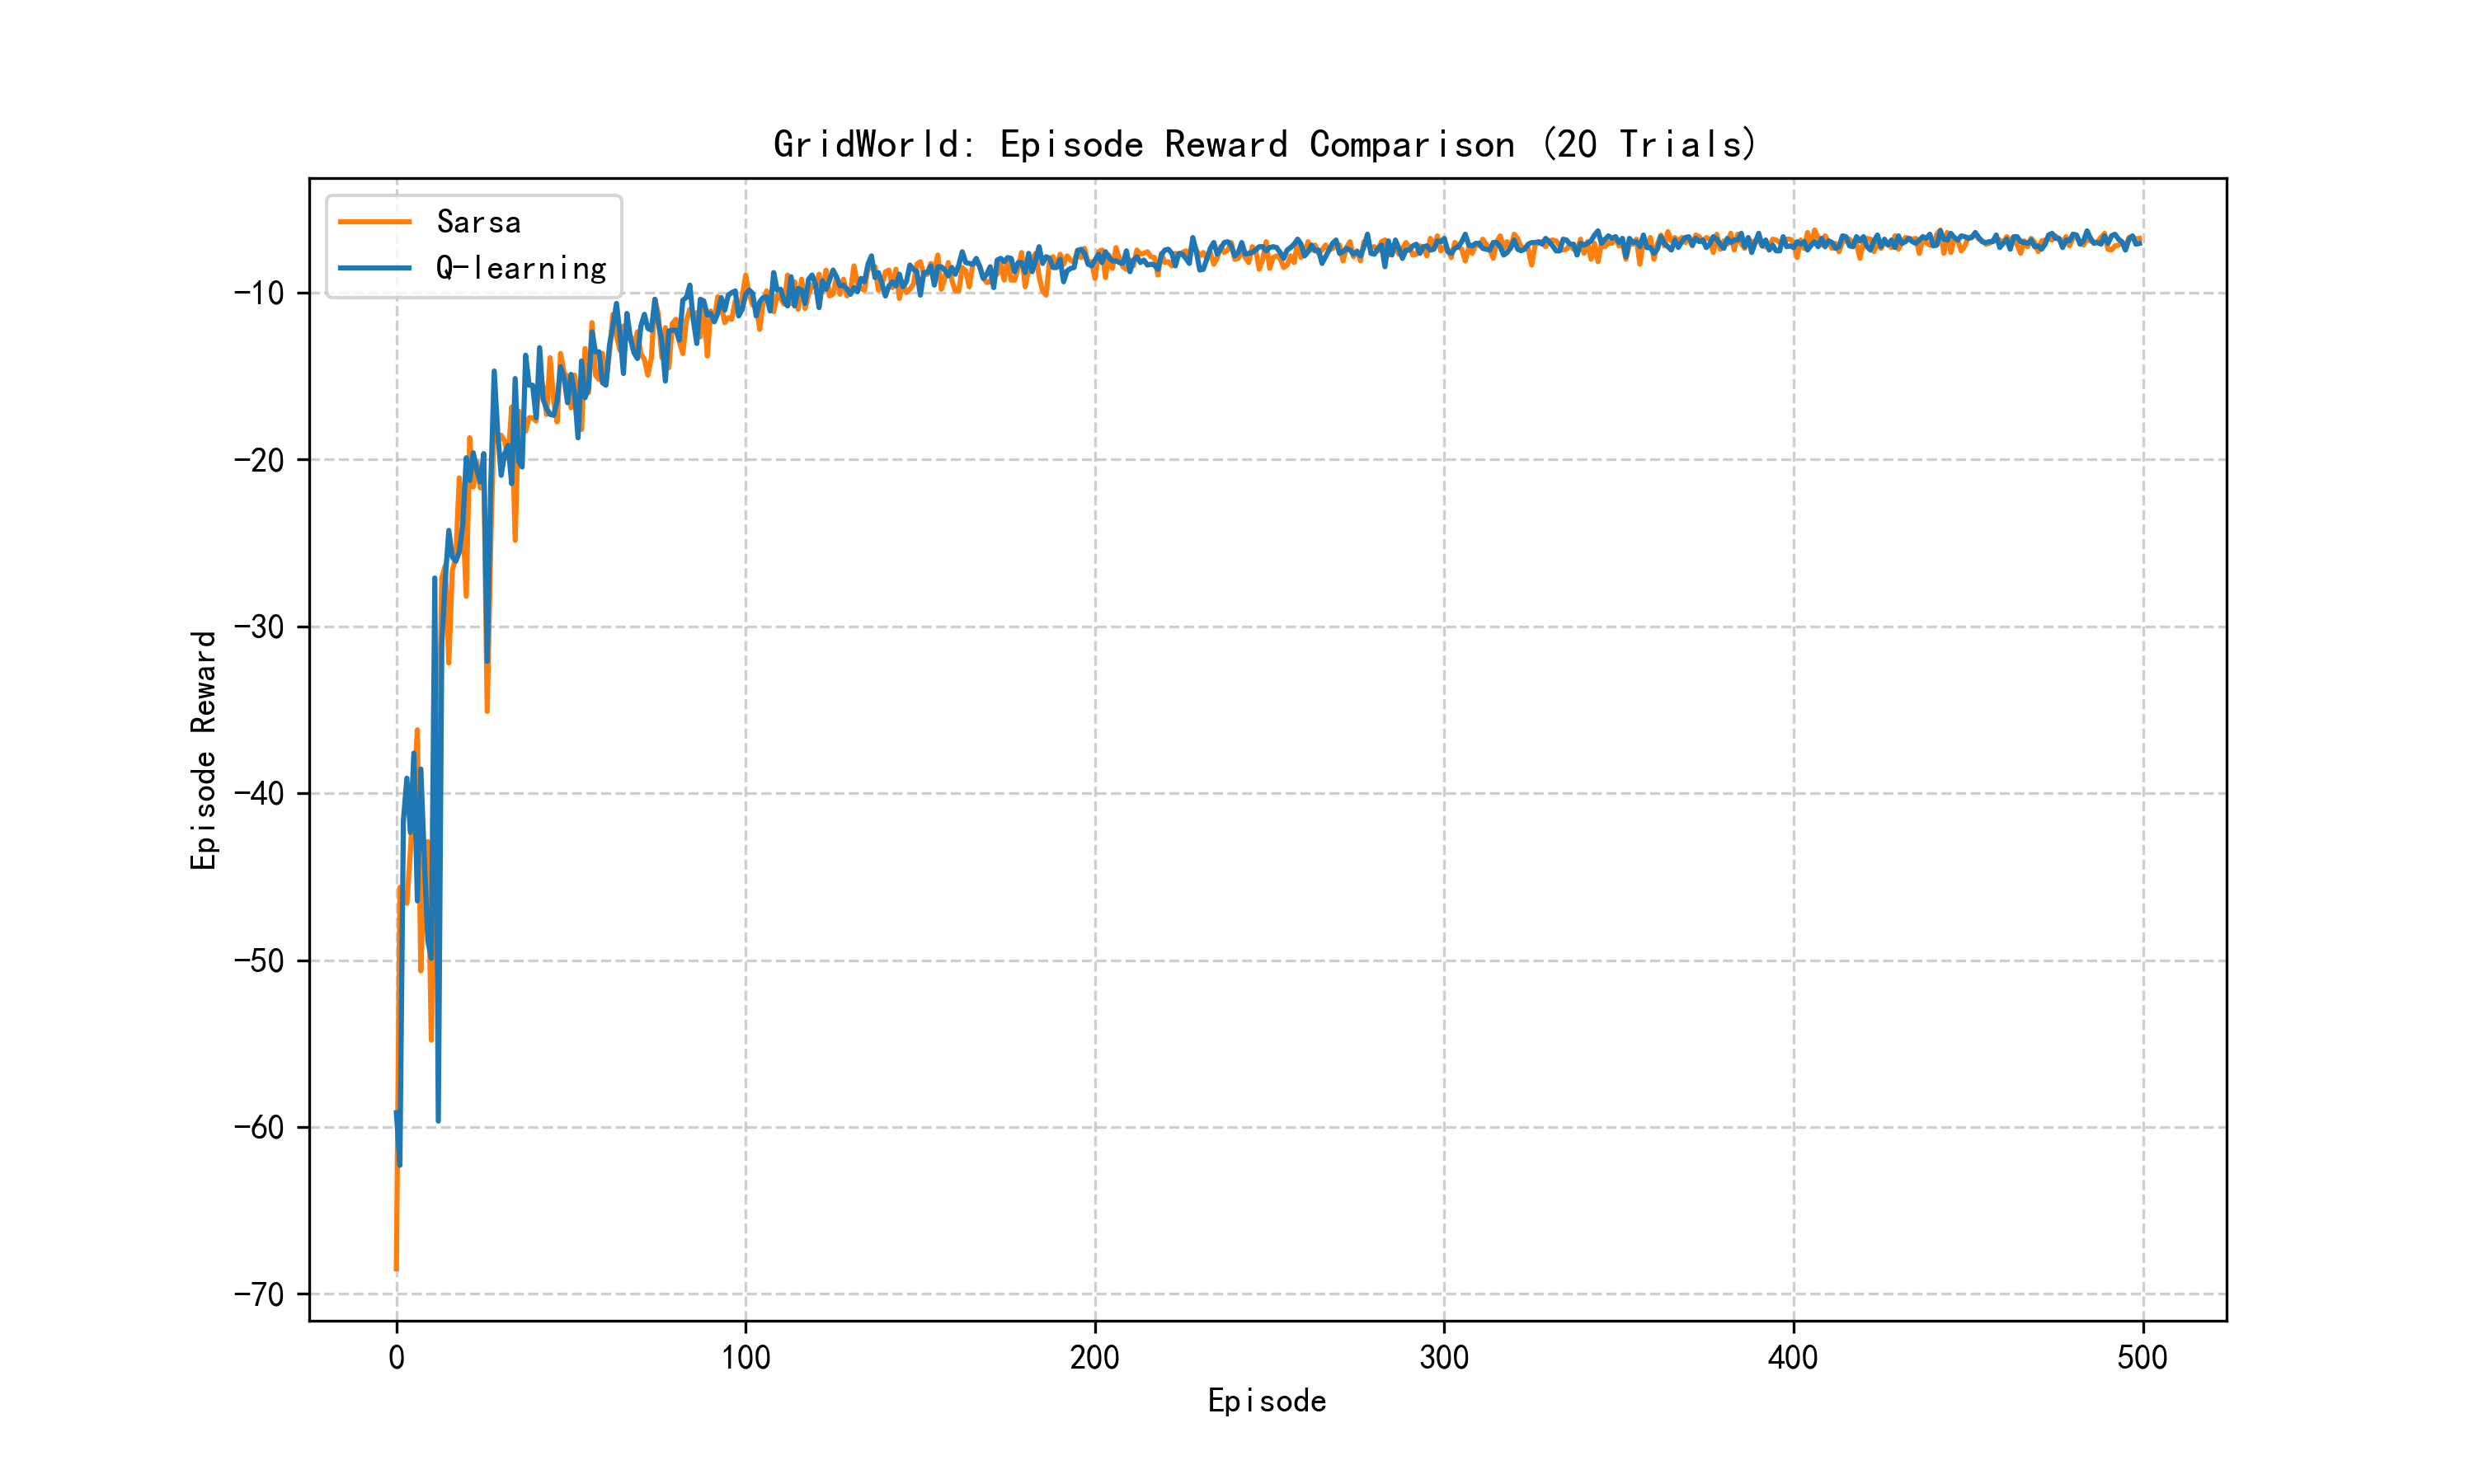
\includegraphics[width=\linewidth]{exp4/results/task4_grid_rewards.png}
\end{minipage}\hfill
\begin{minipage}{0.49\textwidth}
\centering
\textbf{到达目标步数}\\[0.4em]
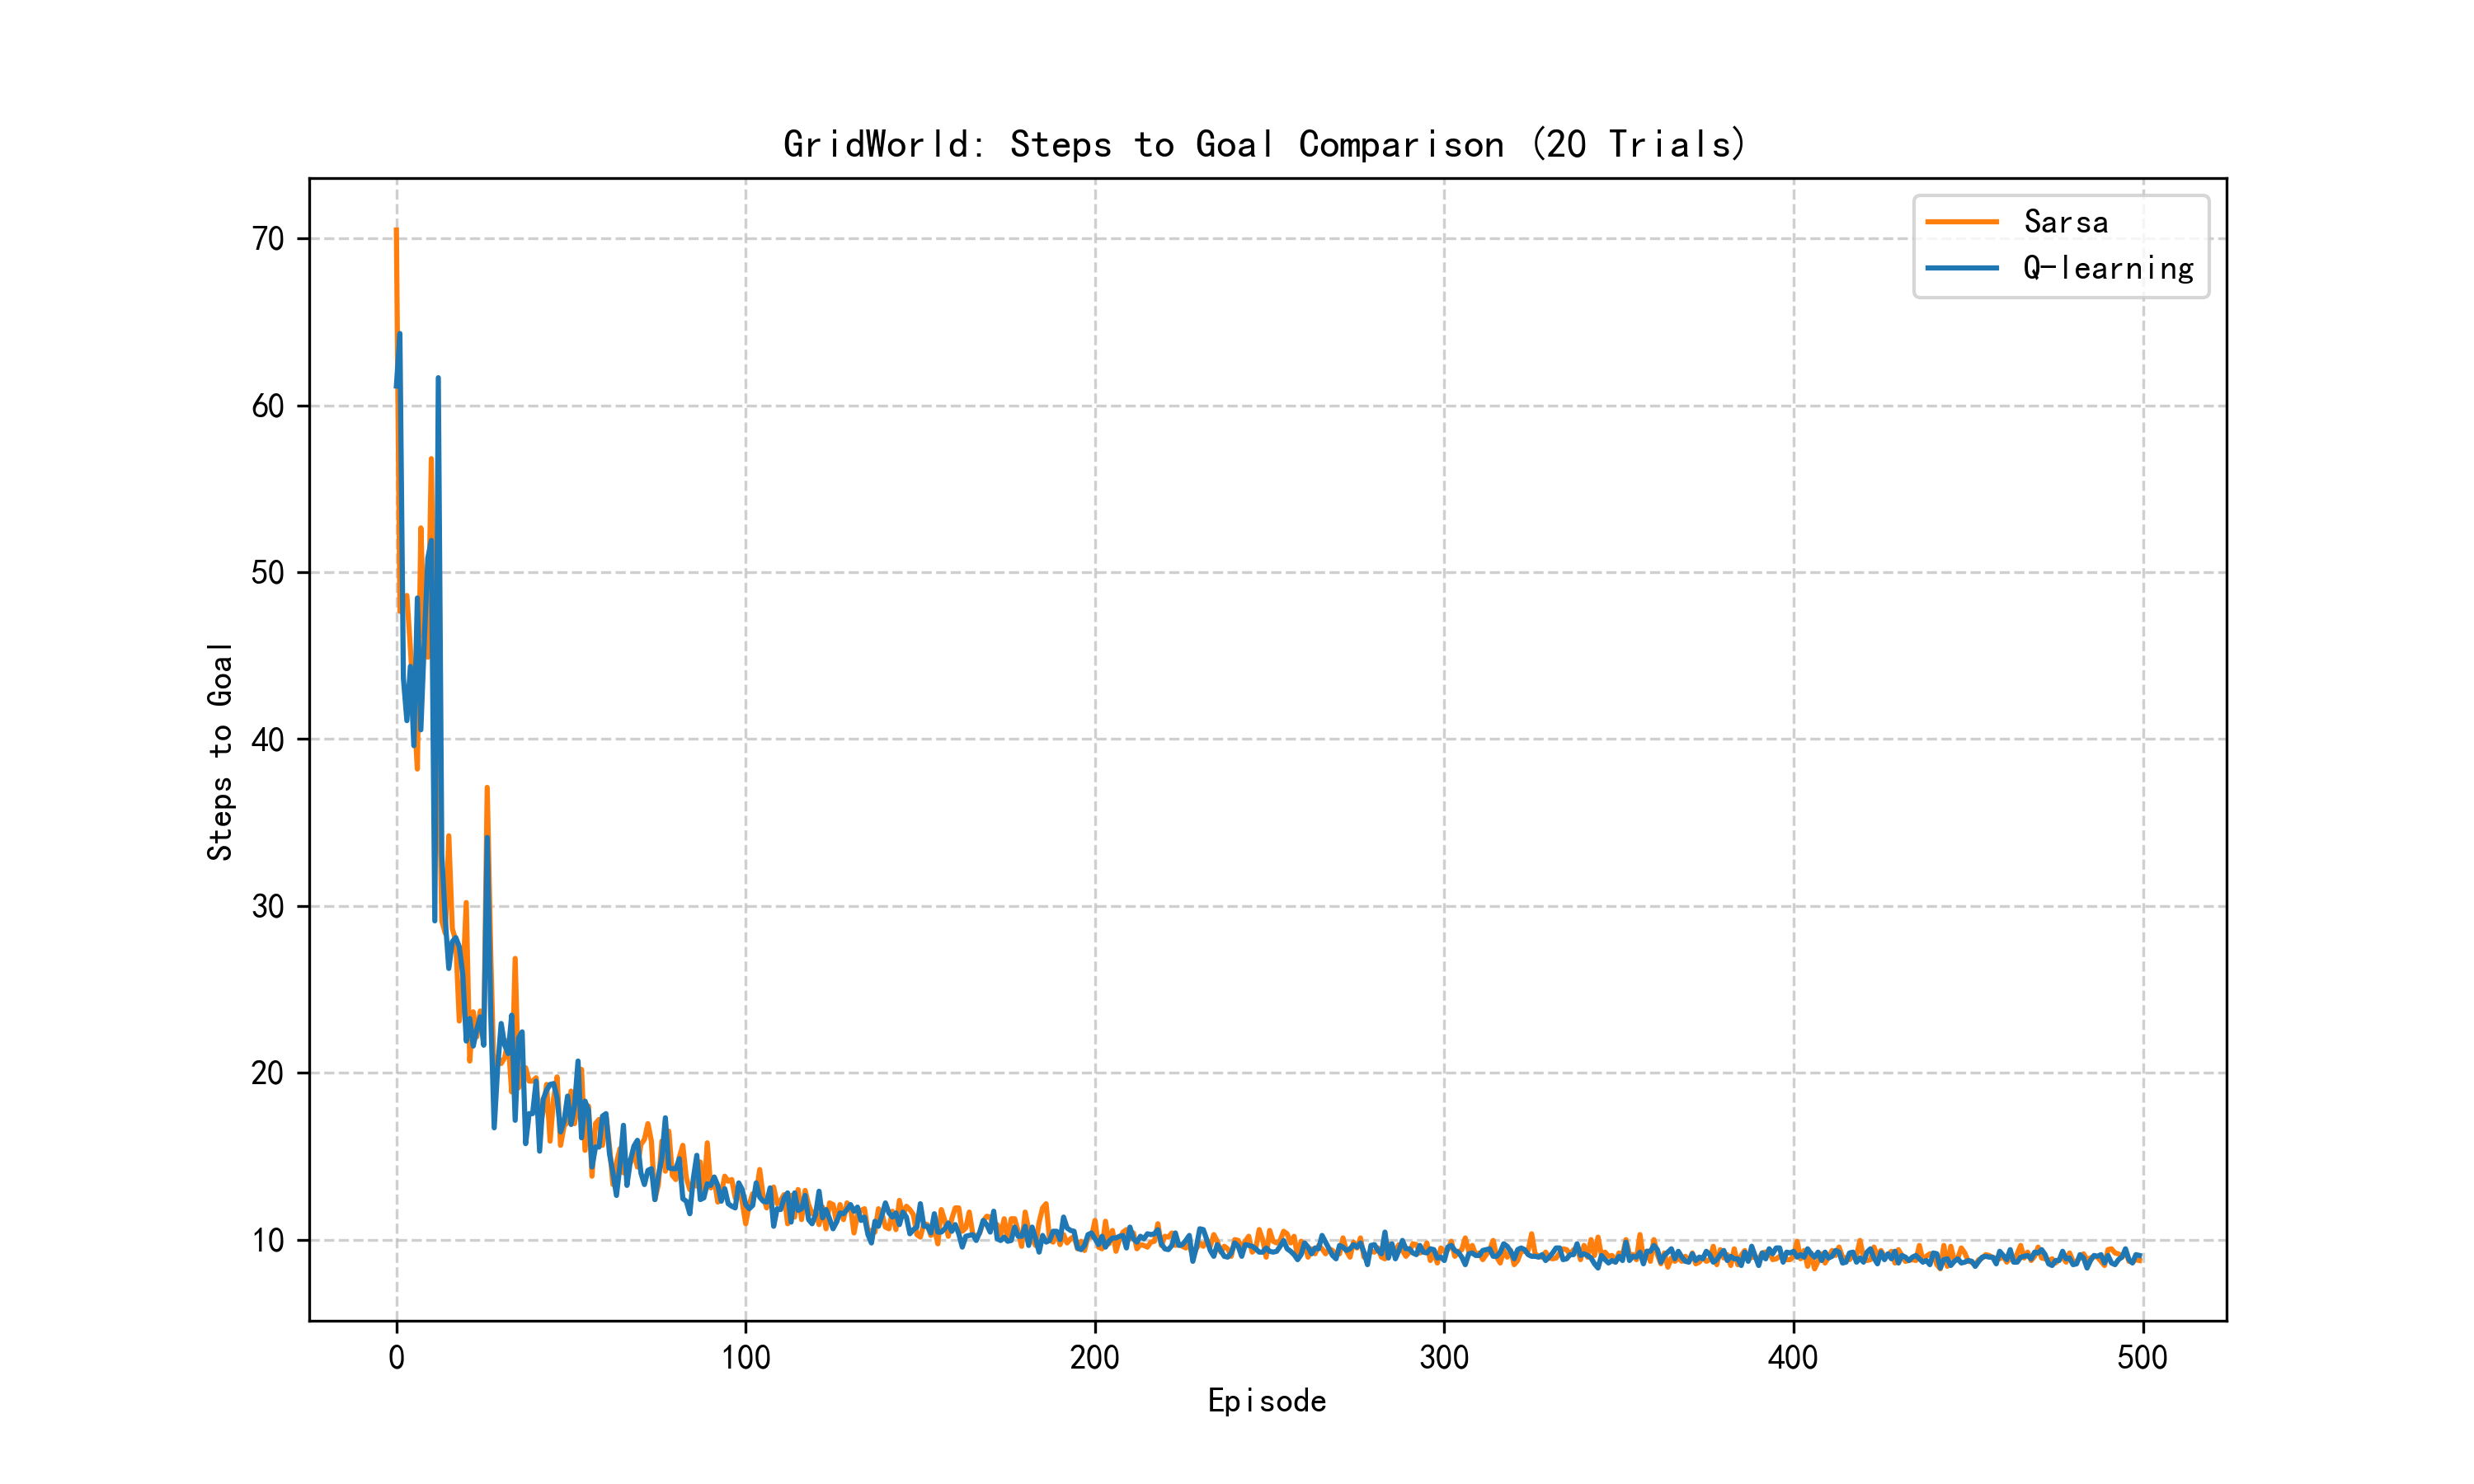
\includegraphics[width=\linewidth]{exp4/results/task4_grid_steps.png}
\end{minipage}
\caption{GridWorld 中 Q-learning 与 Sarsa 的学习曲线}
\end{figure}

\begin{figure}[H]
\centering
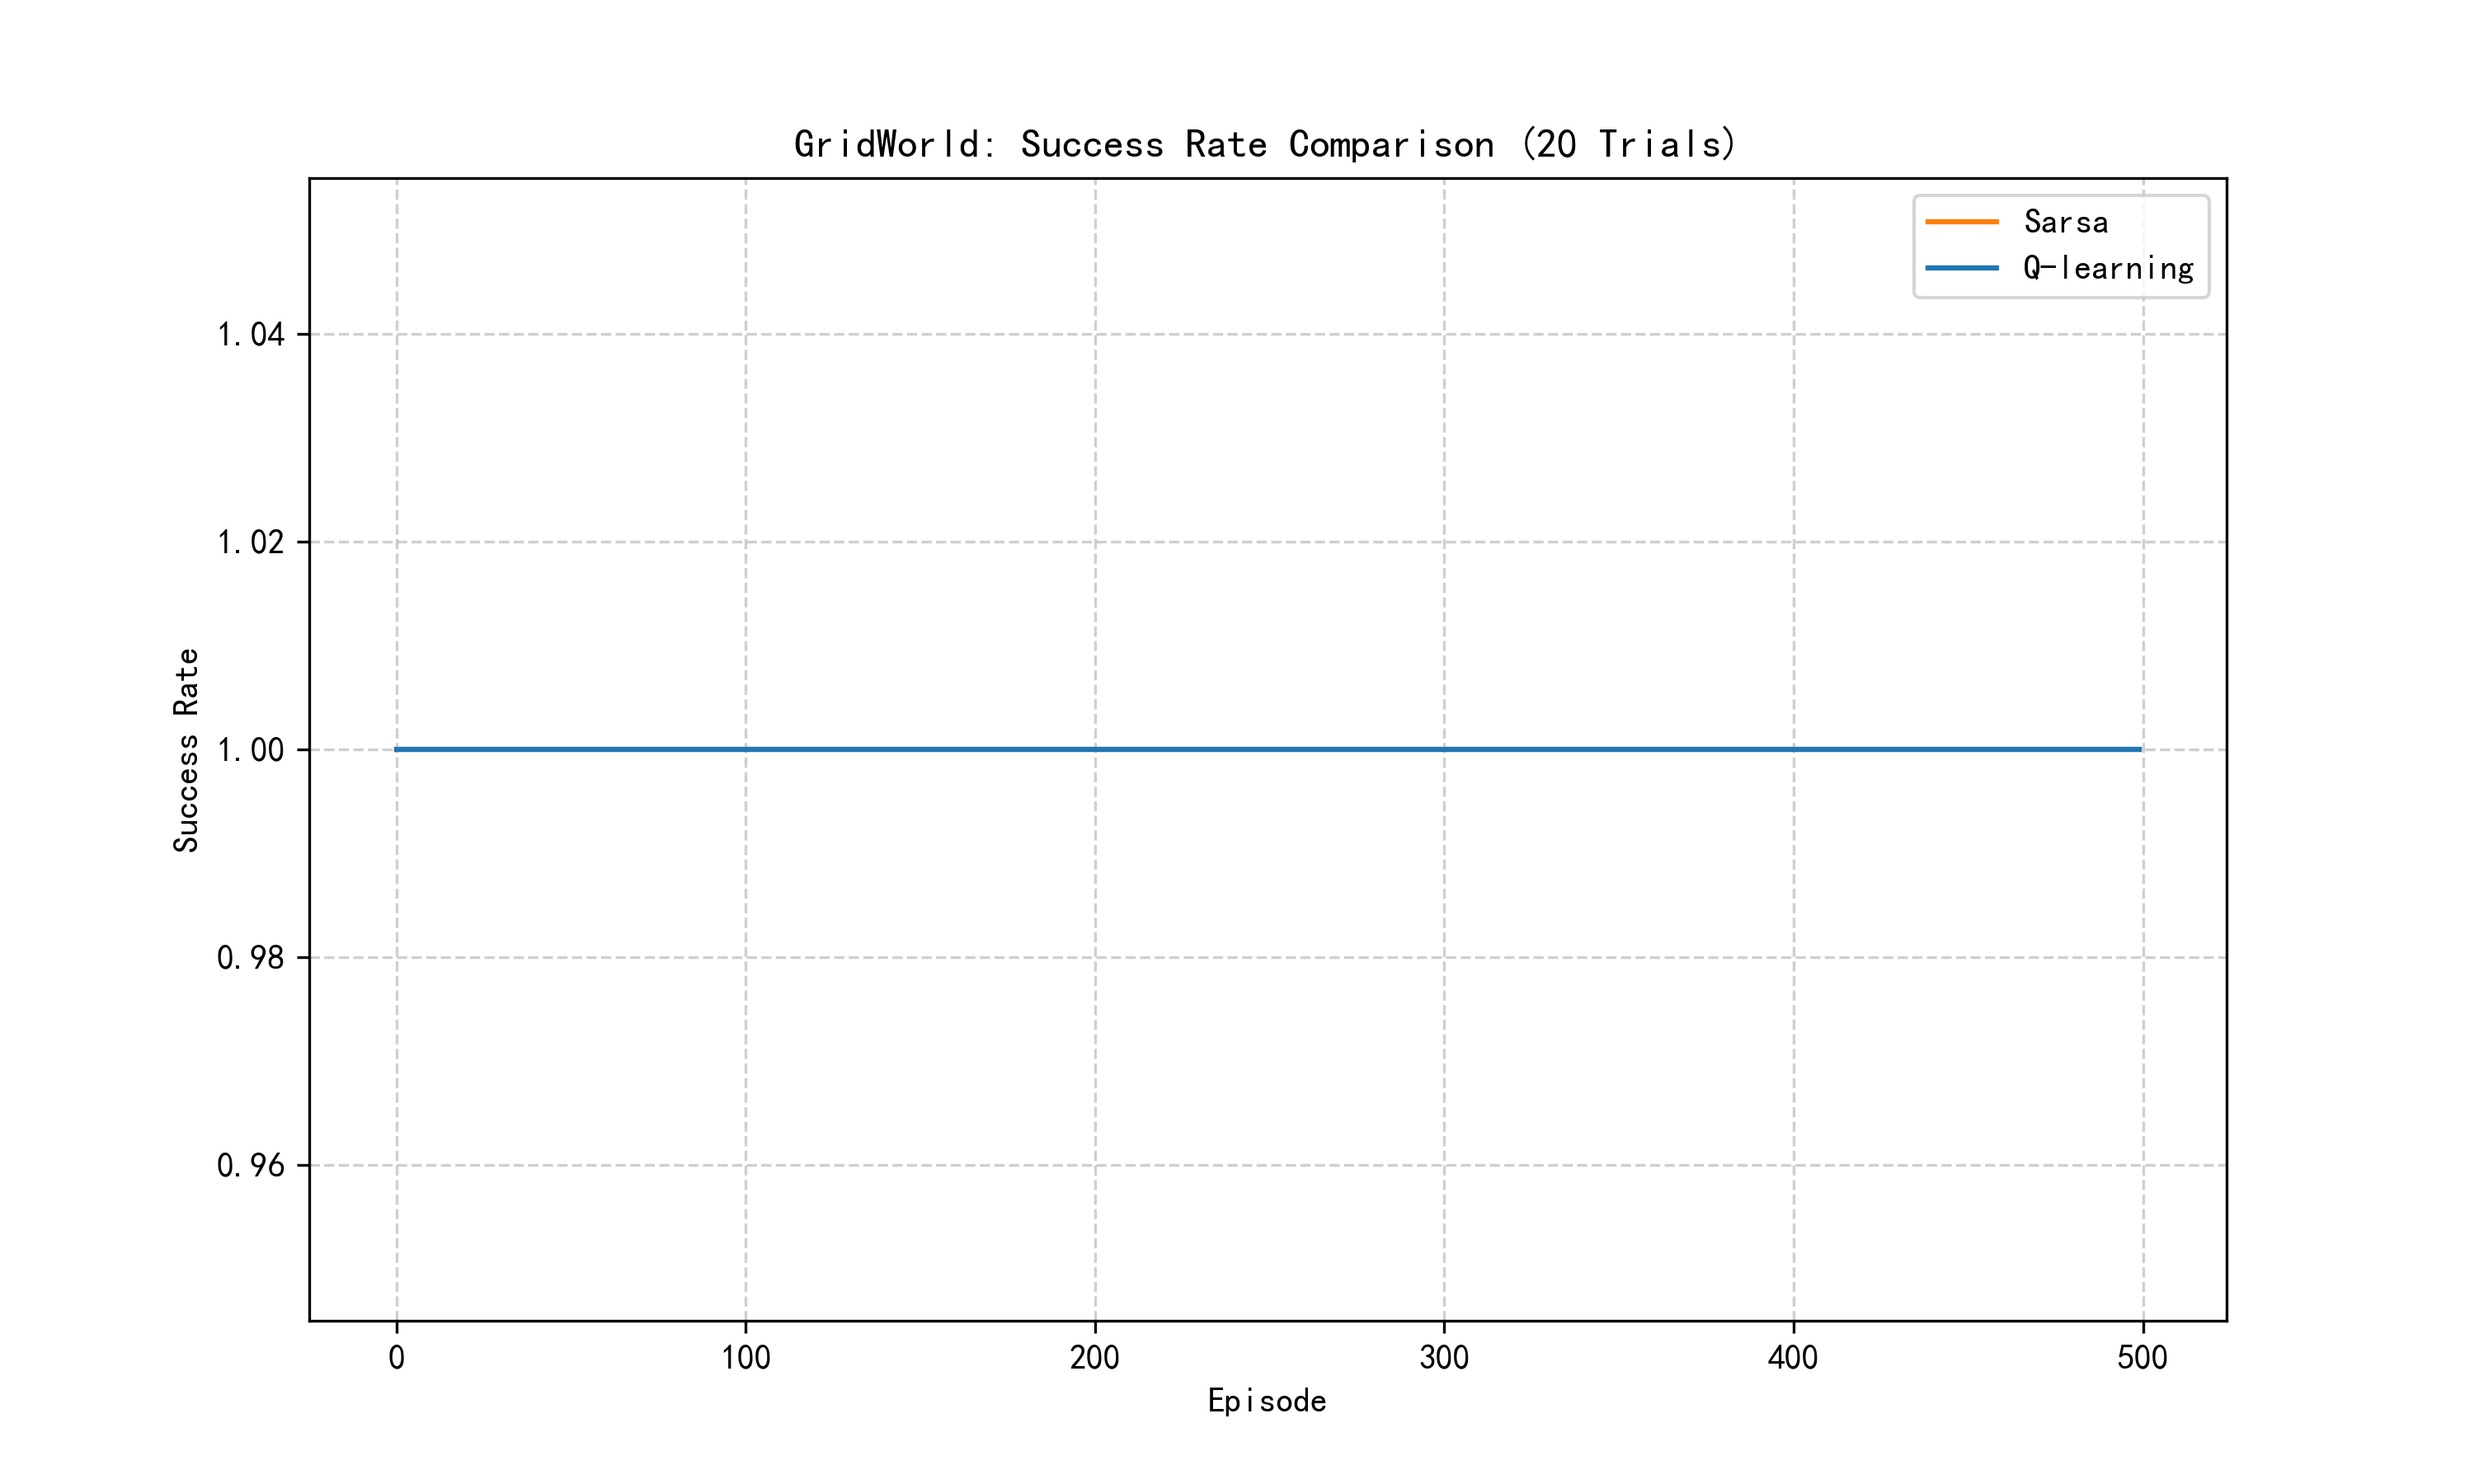
\includegraphics[width=0.55\textwidth]{exp4/results/task4_grid_success_rate.png}
\caption{Q-learning 与 Sarsa 成功率对比曲线}
\end{figure}

以下是 Trial 0 结束后，Q-learning 与 Sarsa 的最终贪心策略箭头图：

\begin{figure}[H]
\centering
\begin{minipage}{0.49\textwidth}
\centering
\textbf{Sarsa 最终策略}\\[0.4em]
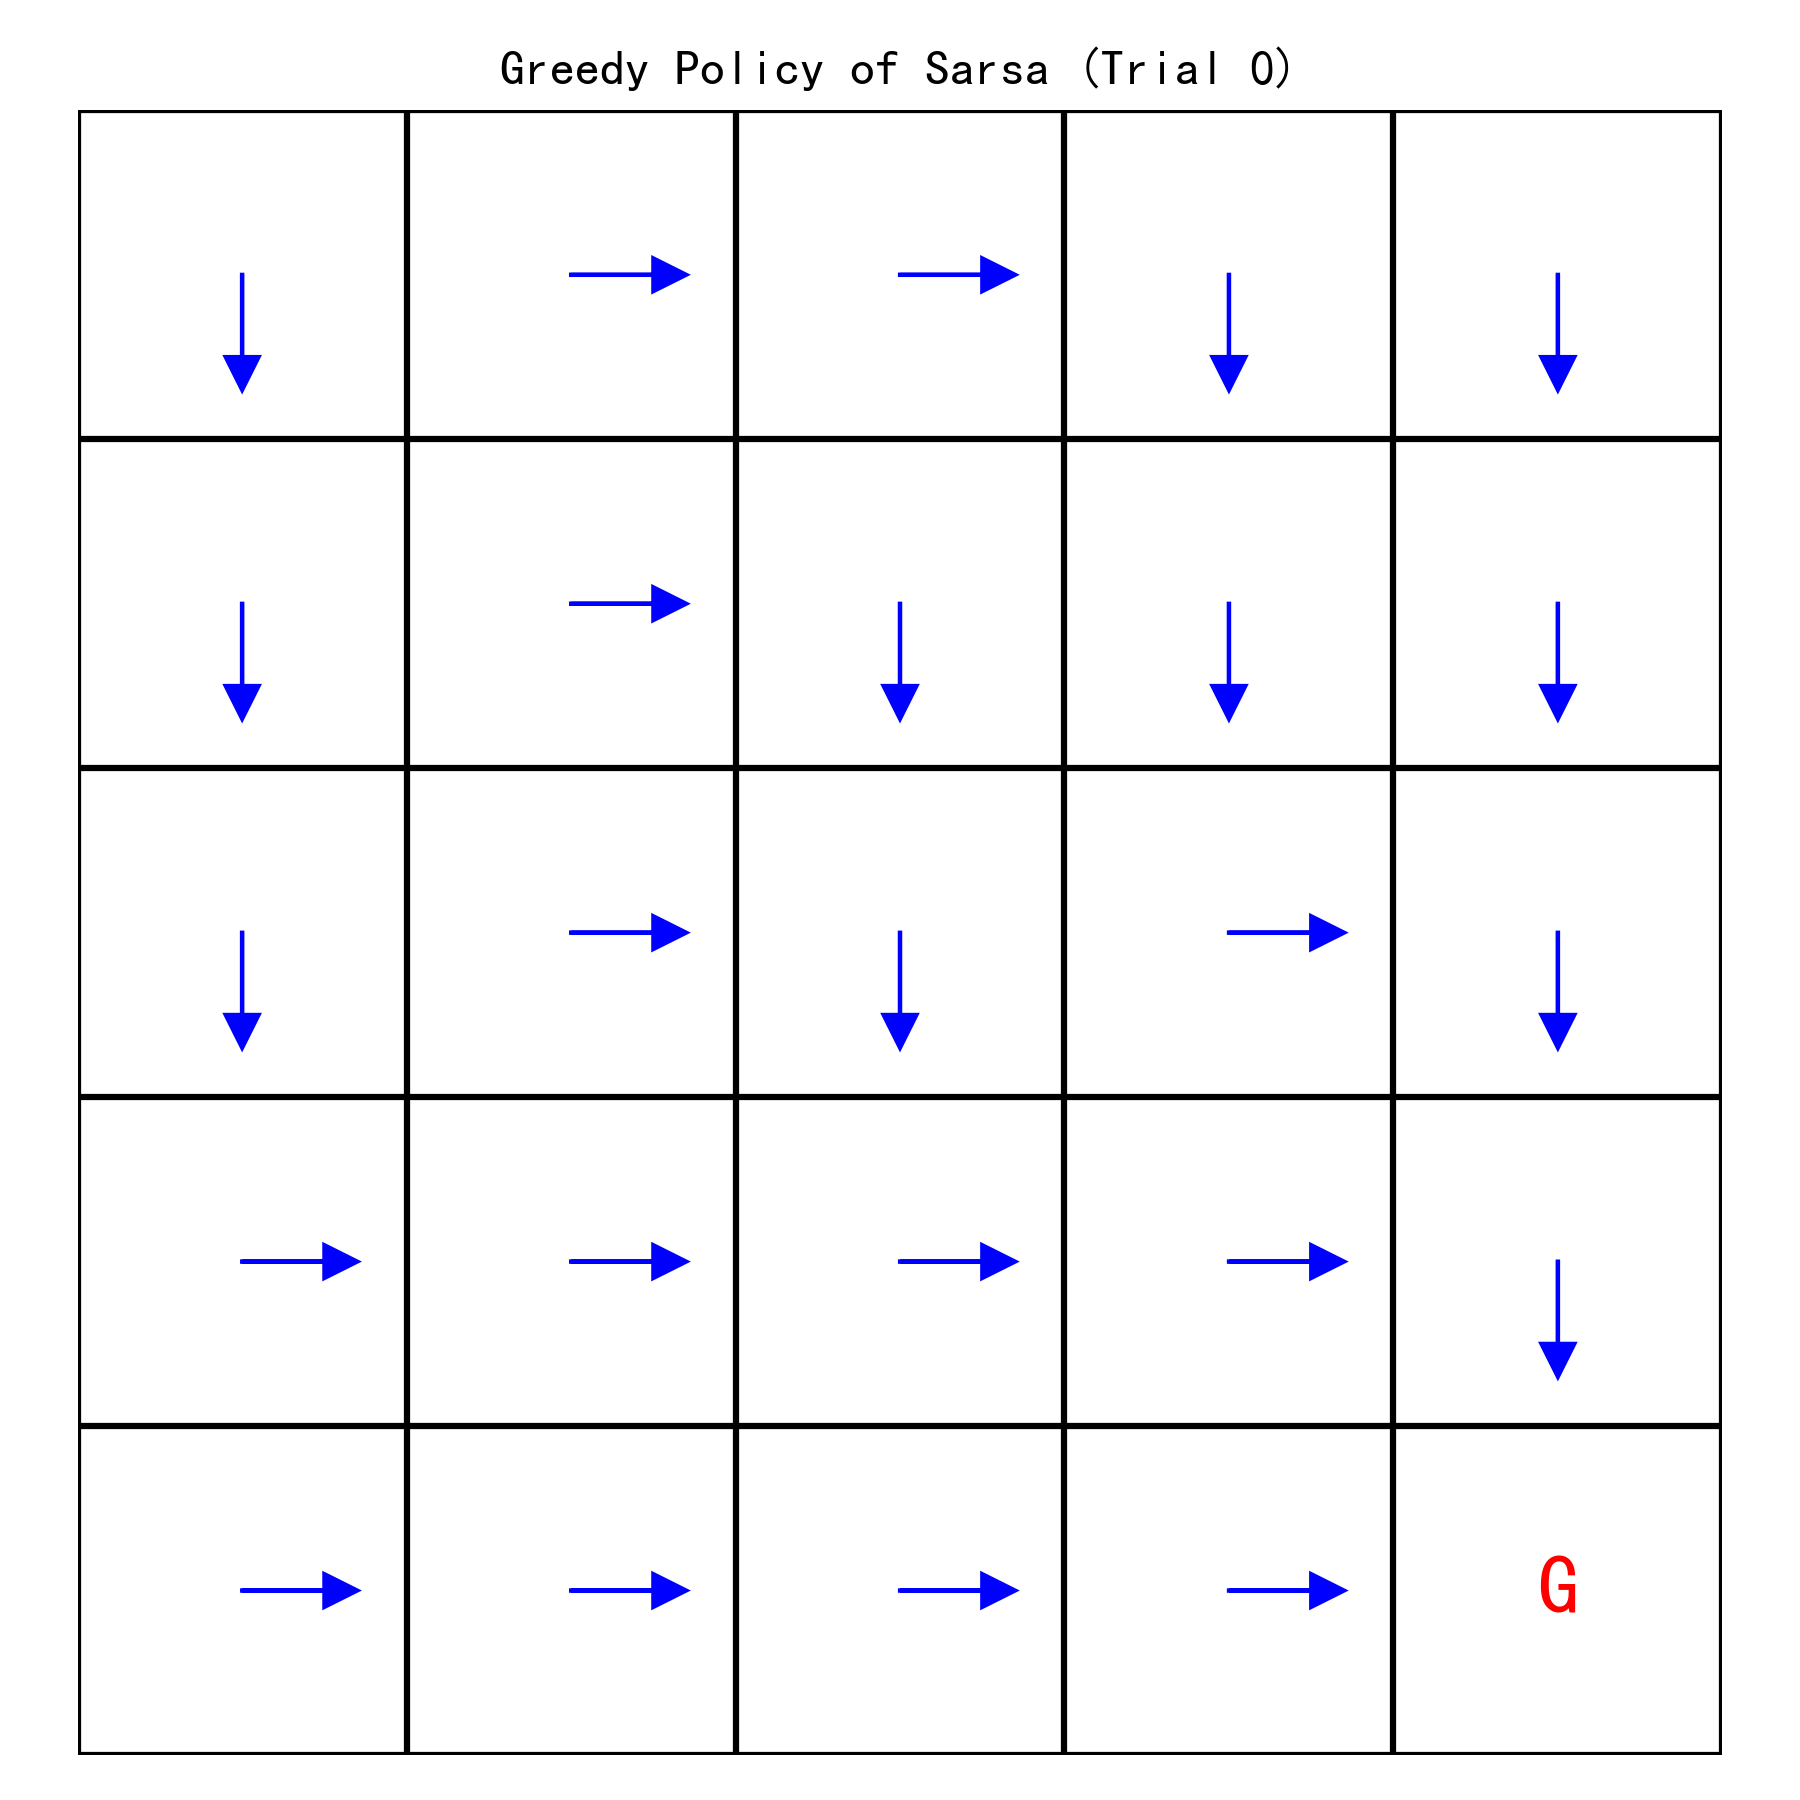
\includegraphics[width=\linewidth]{exp4/results/task4_grid_sarsa_policy.png}
\end{minipage}\hfill
\begin{minipage}{0.49\textwidth}
\centering
\textbf{Q-learning 最终策略}\\[0.4em]
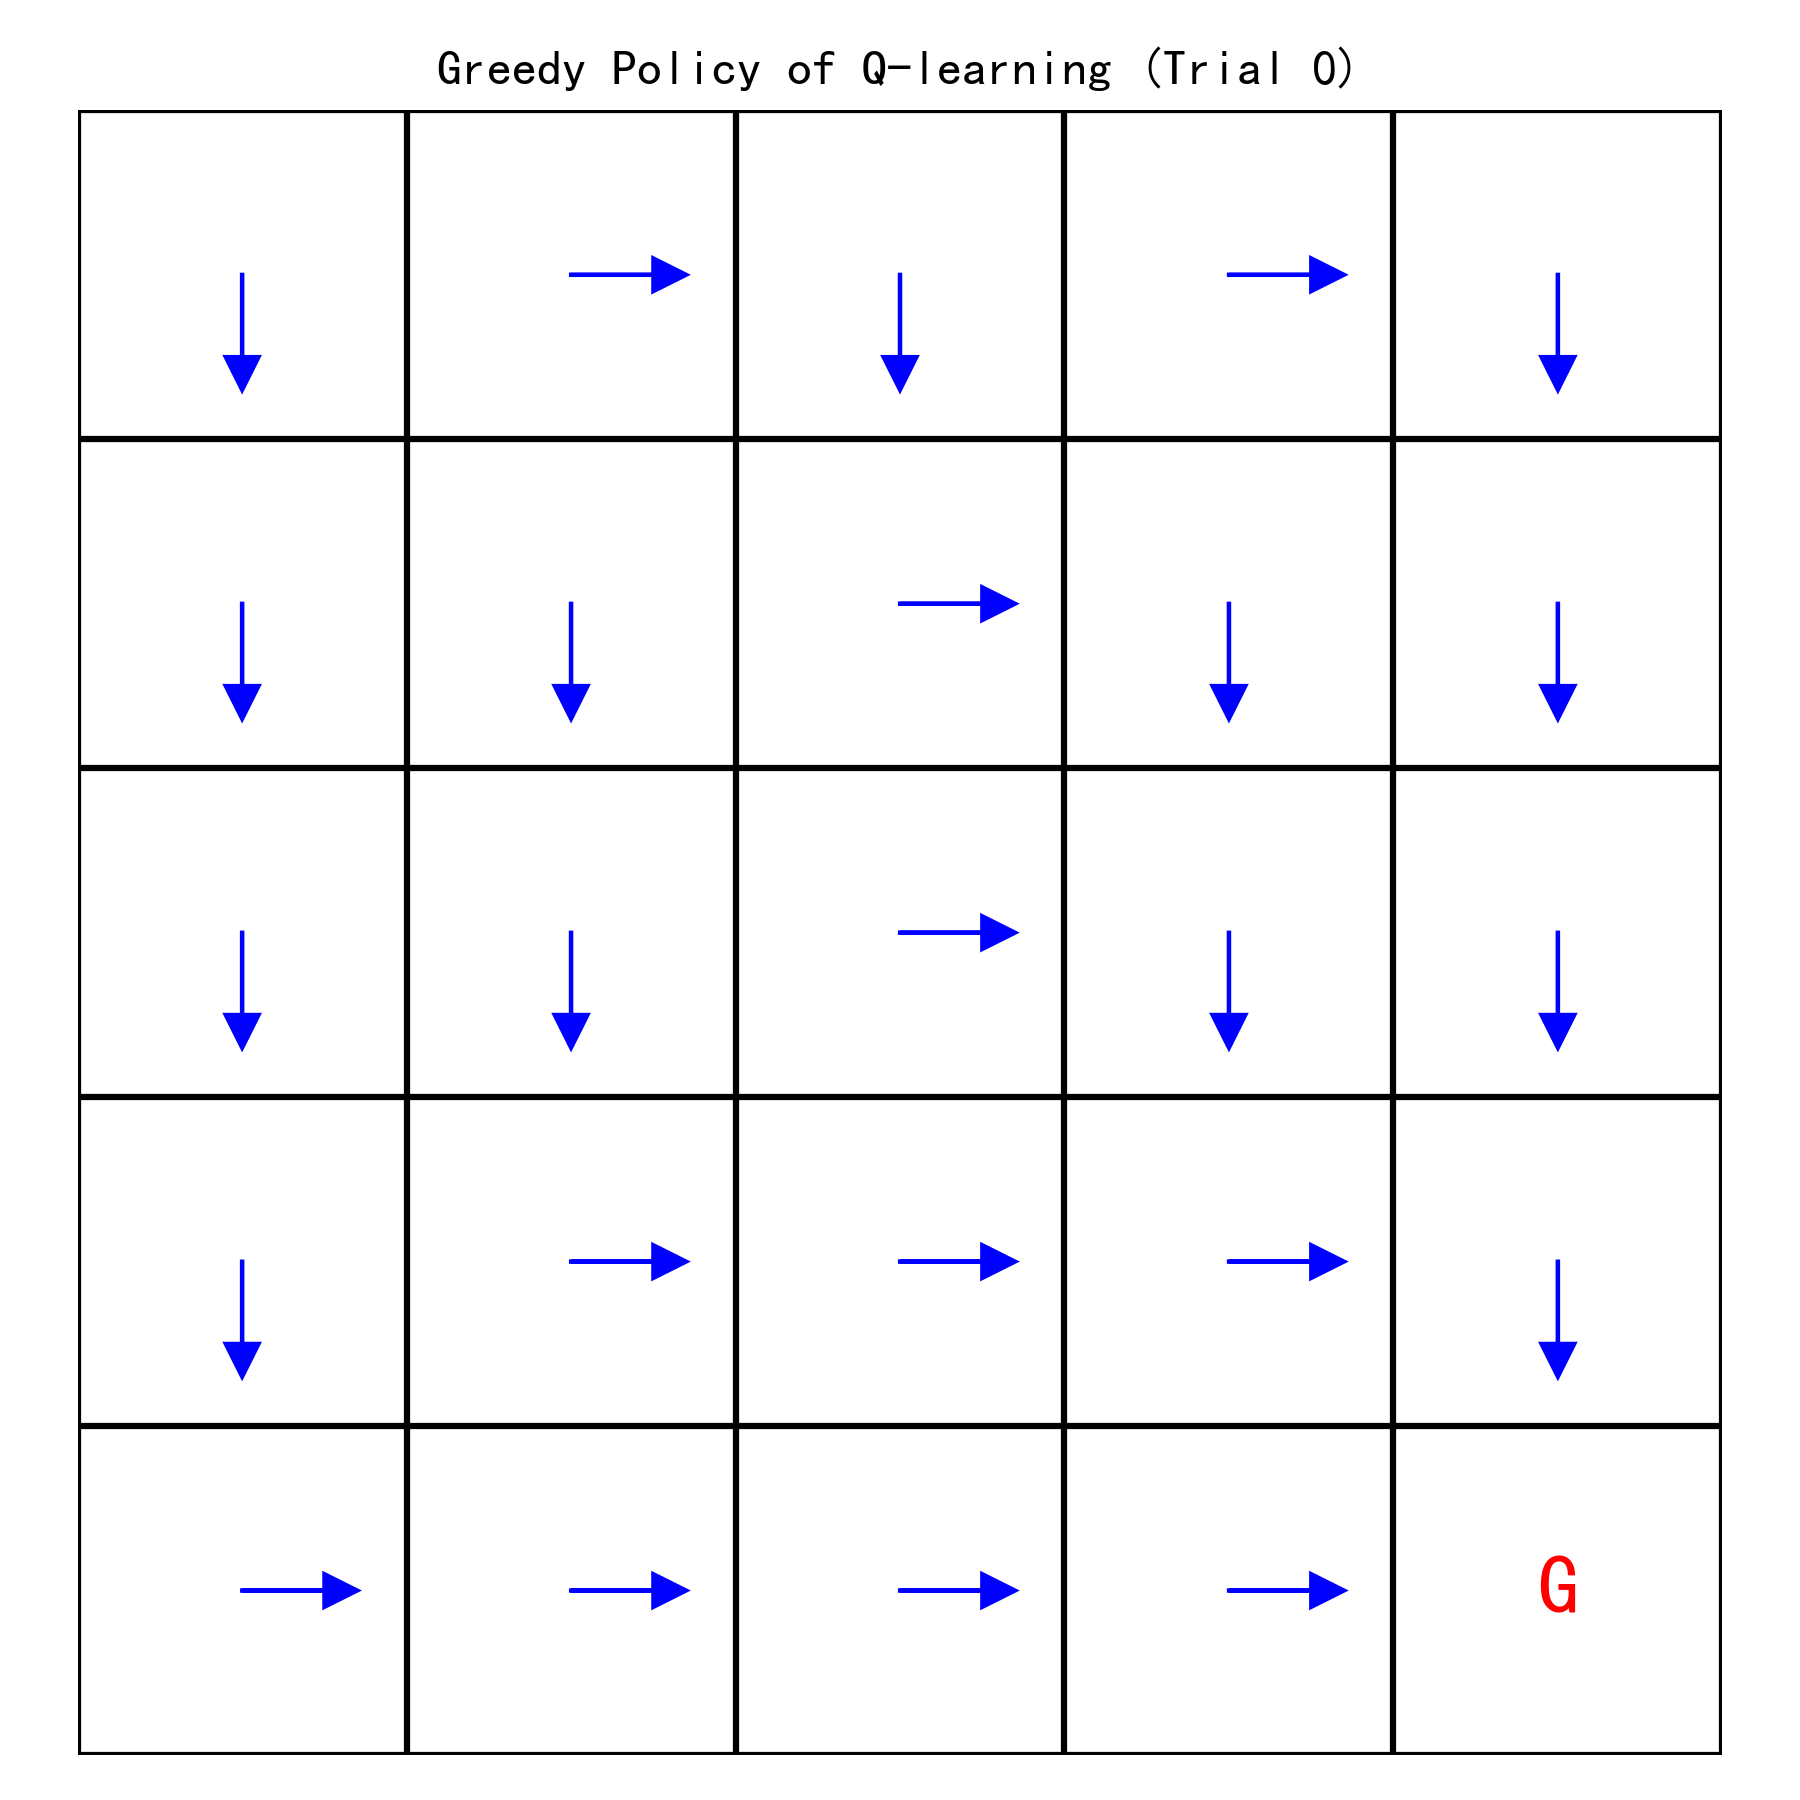
\includegraphics[width=\linewidth]{exp4/results/task4_grid_q_policy.png}
\end{minipage}
\caption{GridWorld 中 Sarsa 与 Q-learning 的最终策略}
\end{figure}

\paragraph{结果分析}
在确定性的 $5\times5$ GridWorld 中，两种算法的曲线接近，均在约 80 个 episode 后达到 100\% 成功率，最终策略均形成从起点到目标的最短路径。该环境不存在会明显区分探索风险的高惩罚区域，因此本实验未观察到显著的收敛速度或稳定性差异。

这一结果说明两种 TD 目标在当前任务上都能完成控制学习，但不能据此推断它们在所有环境中的表现相同。Sarsa 的目标包含行为策略实际选择的下一动作，Q-learning 的目标使用贪心动作价值；当探索动作的后果差异较大时，两者可能产生不同策略。

\paragraph{思考题}


\question{问题 1：Q-learning 与 Sarsa 的 TD 目标有什么核心区别？为什么 Q-learning 可以学习目标贪心策略而行为策略仍保持探索？}

\answerlabel Sarsa 使用行为策略实际选择的下一动作：
\[
\text{Target}_{\text{Sarsa}}
=R_{t+1}+\gamma Q(S_{t+1},A_{t+1}).
\]
因此，其更新目标包含 $\epsilon$-greedy 探索动作的影响，属于同策略学习。

Q-learning 使用下一状态的最大动作价值：
\[
\text{Target}_{\text{Q-learning}}
=R_{t+1}+\gamma\max_a Q(S_{t+1},a).
\]
生成样本时仍可使用 $\epsilon$-greedy 行为策略探索，但更新时按贪心动作构造目标。只要交互过程能够充分访问相关状态--动作对，Q-learning 就可以在保持探索的同时逼近贪心目标策略的动作价值。

\question{问题 2：在本实验中，Q-learning 是否比 Sarsa 收敛更快或更不稳定？结合曲线说明原因。}

\answerlabel 从累计奖励、到达目标步数和成功率曲线看，Q-learning 与 Sarsa 的收敛轨迹接近，均在约 80 个 episode 后达到 100\% 成功率；本实验没有证据表明 Q-learning 明显更快或更不稳定。

原因在于当前 GridWorld 为确定性环境，且不存在高惩罚风险区域。两种算法虽然采用不同 TD 目标，但最终都能形成最短路径，探索动作对长期回报的影响不足以造成明显差异。

\question{问题 3：简述同策略（On-policy）与异策略（Off-policy）的核心区别，并分析各自特点。}

\answerlabel 同策略方法使用同一策略生成数据并构造更新目标；异策略方法的行为策略负责生成数据，目标策略负责被评估或改进，两者可以不同。结合本实验，Sarsa 的下一动作来自当前 $\epsilon$-greedy 行为策略，Q-learning 的下一动作价值来自贪心目标策略。

\begin{table}[H]
\centering
\begin{tabular}{cC{6.0cm}C{6.0cm}}
\toprule
维度 & 同策略 (On-policy，如 Sarsa) & 异策略 (Off-policy，如 Q-learning) \\
\midrule
策略关系 & 行为策略与目标策略相同 & 行为策略与目标策略可以不同 \\
更新特点 & 更新目标反映当前行为，包括探索动作 & 更新目标可按目标策略构造 \\
主要影响 & 学到的是当前行为策略的价值 & 能分离探索与目标策略，但需满足覆盖等条件 \\
\bottomrule
\end{tabular}
\end{table}

\subsection{核心代码与分析}

\subsubsection{GridWorld 环境状态转移与奖励 (env.py)}
以下是网格环境的 \texttt{step} 实现。程序准确处理了边界碰撞和目标状态的终止逻辑：
\begin{lstlisting}[language=python]
def step(self, action):
    # 终止状态下无法执行动作，直接返回
    if self.state == self.goal:
        return self.state, 0.0, True, {}    
    r, c = self.state
    # 动作映射：0:上, 1:下, 2:左, 3:右
    if action == 0:    # Up
        nr, nc = r - 1, c
    elif action == 1:  # Down
        nr, nc = r + 1, c
    elif action == 2:  # Left
        nr, nc = r, c - 1
    elif action == 3:  # Right
        nr, nc = r, c + 1    
    bump = False
    # 撞墙边界检查
    if nr < 0 or nr >= self.size or nc < 0 or nc >= self.size:
        nr, nc = r, c
        bump = True    
    self.state = (nr, nc)
    done = (self.state == self.goal)
    # 奖励规则：到达终点得 +1.0，撞墙或普通移动均得 -1.0
    if done:
        reward = 1.0
    else:
        reward = -1.0    
    return self.state, reward, done, {}
\end{lstlisting}

\subsubsection{TD(0) 评估核心更新 (task2\_td0\_eval.py)}
本段展示了单步 TD 误差 $\delta_t = R_{t+1} + \gamma V(S_{t+1}) - V(S_t)$ 的计算与增量式更新：
\begin{lstlisting}[language=python]
# TD(0) 更新核心
# 若 next_state 为 Goal，则 done=True，此时 v_next 强制为 0.0
v_next = V[nr, nc] if not done else 0.0
td_target = reward + env.gamma * v_next
# 更新公式：V(s) <- V(s) + alpha * [ TD_Target - V(s) ]
V[r, c] += lr * (td_target - V[r, c])
\end{lstlisting}

\subsubsection{n-step Sarsa 控制核心更新 (task3\_sarsa.py)}
算法通过数组缓存单步的状态、动作与奖励。在当前时间步超过 $n$ 后，从后往前计算折现累计回报 $G$，并在有终点截断的情况下正确处理自举项：
\begin{lstlisting}[language=python]
tau = t - n + 1
if tau >= 0:
    G = 0.0
    # 计算从 tau+1 到 min(tau+n, T) 的真实折扣回报和
    for i in range(tau + 1, min(tau + n, T) + 1):
        G += (gamma ** (i - tau - 1)) * rewards[i]
    # 若 n 步之内未到终点，则自举加上 tau+n 状态动作对的 Q 值估计
    if tau + n < T:
        s_tn = states[tau + n]
        a_tn = actions[tau + n]
        G += (gamma ** n) * Q[s_tn[0], s_tn[1], a_tn]
    
    # 更新 Q-table
    s_tau = states[tau]
    a_tau = actions[tau]
    Q[s_tau[0], s_tau[1], a_tau] += alpha * (G - Q[s_tau[0], s_tau[1], a_tau])
\end{lstlisting}

\subsubsection{Q-learning 在线更新逻辑 (task4\_qlearning.py)}
Q-learning 使用 $\epsilon$-greedy 行为策略在线选择动作并与环境交互，但 TD 目标使用下一状态的最大动作价值：
\begin{lstlisting}[language=python]
# epsilon-greedy 行为策略负责生成在线交互数据
action = epsilon_greedy(Q[state[0], state[1]], epsilon)
next_state, reward, done, _ = env.step(action)

# 贪心目标策略用于构造 Q-learning 的 TD 目标
next_q = 0.0 if done else np.max(Q[next_state[0], next_state[1]])
td_target = reward + gamma * next_q
Q[state[0], state[1], action] += alpha * (
    td_target - Q[state[0], state[1], action]
)
\end{lstlisting}
\subsection{总结与体会}

本实验完成了 TD(0)、n-step Sarsa、Sarsa 与 Q-learning 的实现和对比，得到以下结论：
\begin{enumerate}
\item TD(0) 在本实验中比 FV-MC 更快降低 RMSE；固定步长较大时前期下降更快，但后期波动也更明显。
\item n-step Sarsa 中，$n=3$ 和 $n=5$ 比 $n=1$ 更早达到稳定成功率，说明多步回报加快了当前 GridWorld 中的奖励传播；该结果不能直接推广到其他环境。
\item Sarsa 与 Q-learning 在当前确定性 GridWorld 中均于约 80 个 episode 后达到 100\% 成功率，未表现出明显的速度或稳定性差异。两者的关键区别仍在 TD 目标：Sarsa 使用实际下一动作，Q-learning 使用下一状态的最大动作价值。
\end{enumerate}

\newpage
\section{值函数近似}

\subsection{实验目的与要求}
\begin{enumerate}
\item 理解值函数近似的核心思想：掌握从表格表示到参数化函数表示的必要性与优势。
\item 掌握基于函数近似的状态值估计算法：能够使用线性函数近似实现 TD(0) 算法（TD-Linear）。
\item 掌握基于函数近似的控制算法：能够实现基于函数近似的 Sarsa 和 Q-learning，并理解其与表格版本的区别。
\item 理解深度 Q-learning 的基本机制：包括目标网络和经验回放的作用。
\end{enumerate}
\subsection{实验内容与设计}

\subsubsection{公共环境与特征设置}

各任务使用相同的 $5\times5$ GridWorld 和 $\gamma=0.9$。线性近似以状态坐标构造特征，并对高阶特征进行归一化；控制任务将状态特征与动作独热编码组合为联合特征。评价时同时报告策略性能和近似误差，避免仅凭训练回报判断价值函数质量。

\subsubsection{任务 1：状态值近似设计}

在均匀随机策略下比较 TD-Table 与 TD-Linear，并测试 3 维、6 维和 10 维特征。使用动态规划价值作为基准，记录 RMSE 曲线和最终误差，以分析特征表达能力对近似偏差的影响。

\subsubsection{任务 2--3：线性控制算法设计}

在相同联合特征、$\epsilon$-greedy 策略和训练环境下实现函数近似 Sarsa 与 Q-learning。通过总奖励、成功率、最短路径长度和最终策略比较同策略与异策略目标；同时观察函数近似下是否出现震荡或发散。

\subsubsection{任务 4：DQN 实验设计}

DQN 使用状态坐标作为输入、单隐藏层网络输出四个动作值，回放缓冲区大小为 500，目标网络每 50 步同步。实验使用相同规模的交互数据与表格 Q-learning 对比，并分别分析经验回放和目标网络对训练稳定性的作用。




\subsection{实验过程、结果与分析}

\subsubsection{任务 1：从表格到函数——状态值估计}

函数近似将表格型价值函数 $V(s)$ 替换为参数化函数 $\hat{v}(s, \mathbf{w}) = \mathbf{w}^\top \mathbf{x}(s)$，其中 $\mathbf{x}(s)$ 为手工设计的状态特征向量（如坐标归一化、距目标曼哈顿距离等）。通过对 TD 误差进行半梯度下降来更新参数 $\mathbf{w}$，实现对连续或大规模状态空间的泛化。

在均匀随机行为策略下，我们使用动态规划计算出精确的基准状态价值（True State Values），然后分别运行表格型 TD（TD-Table，学习率 $\alpha=0.05$）和线性函数近似 TD（TD-Linear，学习率 $\alpha=0.001$）进行 2000 个 Episodes 的策略评估。

\paragraph{实验设置}
线性近似特征设计如下：
\begin{itemize}
\item \textbf{3维特征}：$\phi(s) = [1, x, y]^T$
\item \textbf{6维特征}：$\phi(s) = [1, x, y, x^2, y^2, xy]^T$
\item \textbf{10维特征}：$\phi(s) = [1, x, y, x^2, y^2, xy, x^3, y^3, x^2y, xy^2]^T$
\end{itemize}

其中坐标 $(x,y)$ 经归一化映射到区间 $[0.2, 1.0]$ 以防高阶项溢出。

\paragraph{结果数据}
\begin{itemize}
\item \textbf{TD-Table 最终 RMSE}：0.3141
\item \textbf{TD-Linear（3维）最终 RMSE}：0.9892
\item \textbf{TD-Linear（6维）最终 RMSE}：0.5867
\item \textbf{TD-Linear（10维）最终 RMSE}：0.3843
\end{itemize}

各维度的收敛误差曲线及状态价值估计热力图如下：

\begin{figure}[H]
\centering
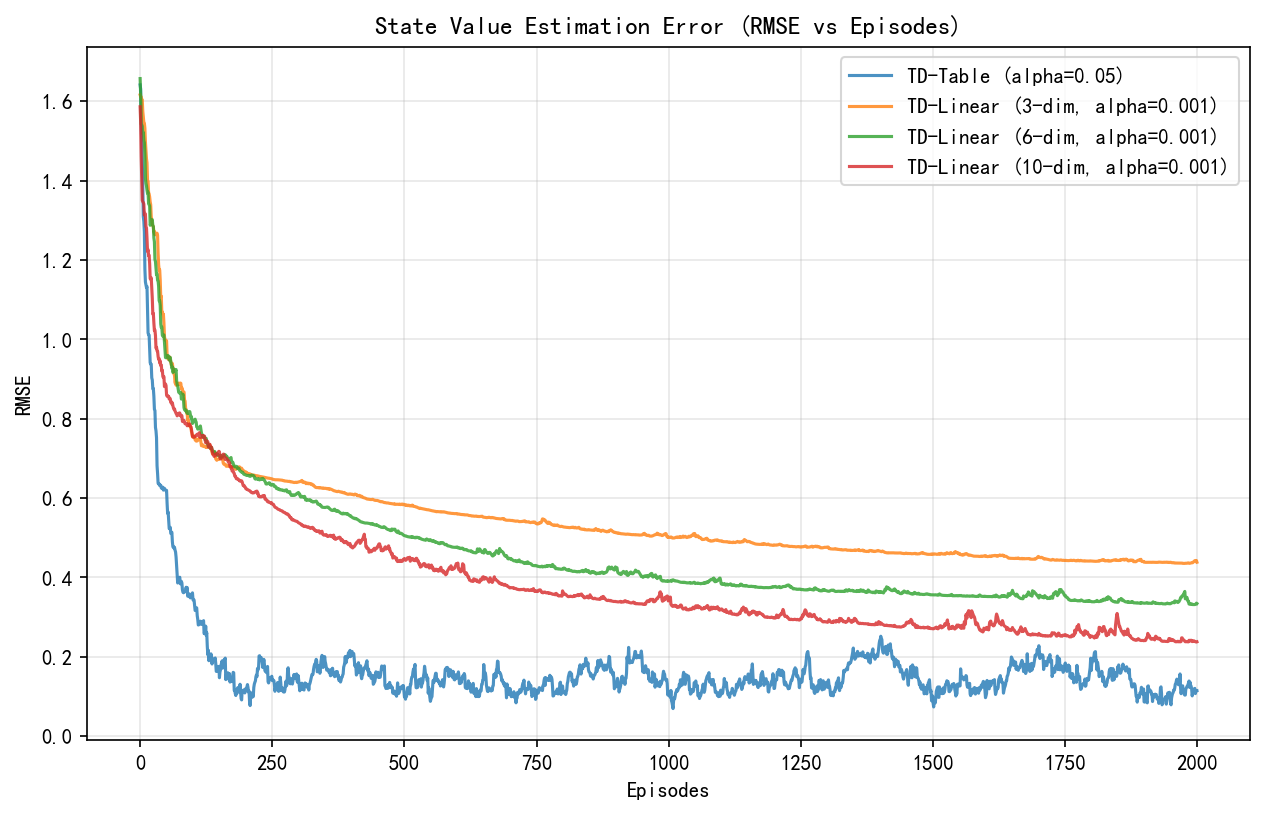
\includegraphics[width=0.75\textwidth]{exp5/results/task1_rmse_comparison.png}
\caption{RMSE 误差对比曲线}
\end{figure}

\begin{figure}[H]
\centering
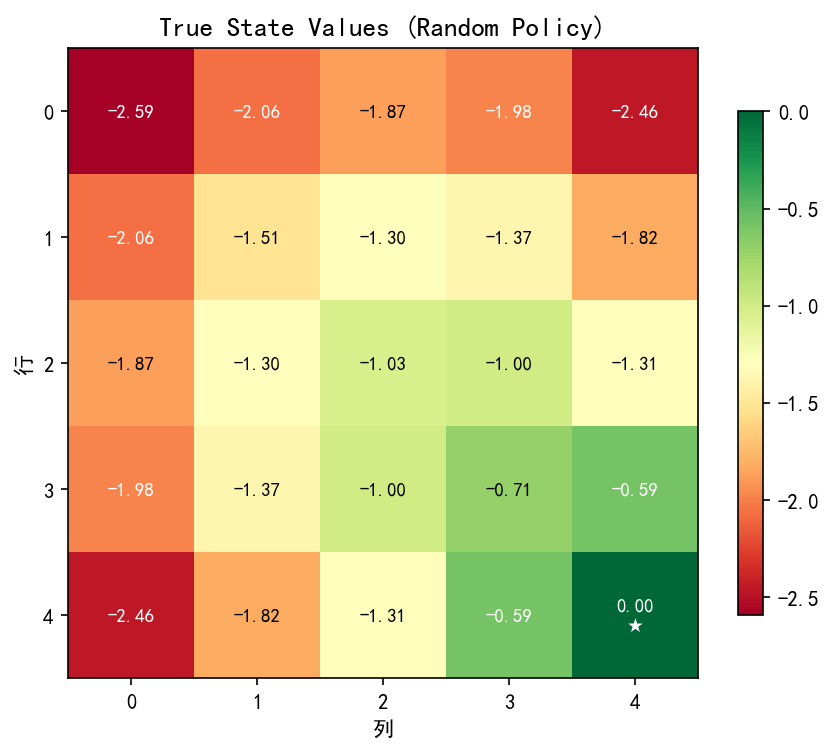
\includegraphics[width=0.4\textwidth]{exp5/results/task1_true_val.png}
\caption{真实状态价值函数 (基准)}
\end{figure}

\begin{figure}[H]
\centering
\begin{minipage}{0.49\textwidth}
\centering
\textbf{TD-Table 状态价值估计}\\[0.4em]
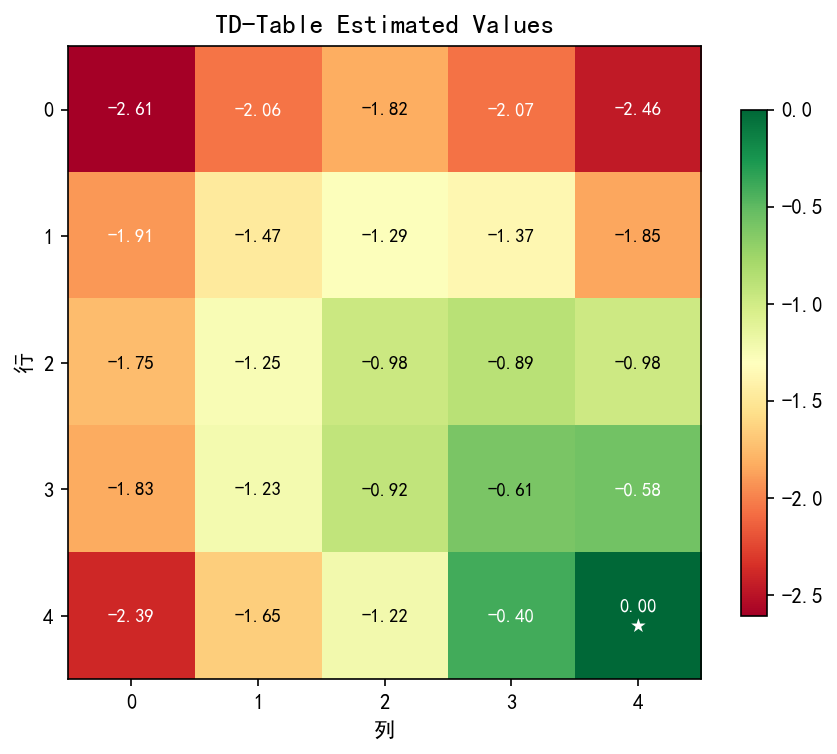
\includegraphics[width=\linewidth]{exp5/results/task1_td_table_val.png}
\end{minipage}\hfill
\begin{minipage}{0.49\textwidth}
\centering
\textbf{TD-Linear（3维）状态价值估计}\\[0.4em]
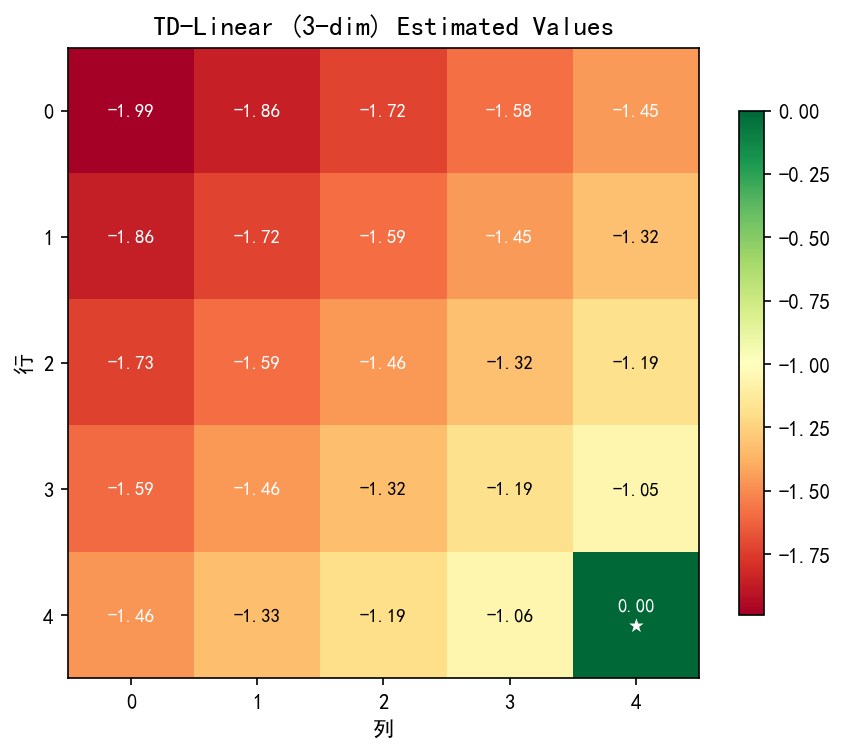
\includegraphics[width=\linewidth]{exp5/results/task1_td_3d_val.png}
\end{minipage}\\[0.8em]
\begin{minipage}{0.49\textwidth}
\centering
\textbf{TD-Linear（6维）状态价值估计}\\[0.4em]
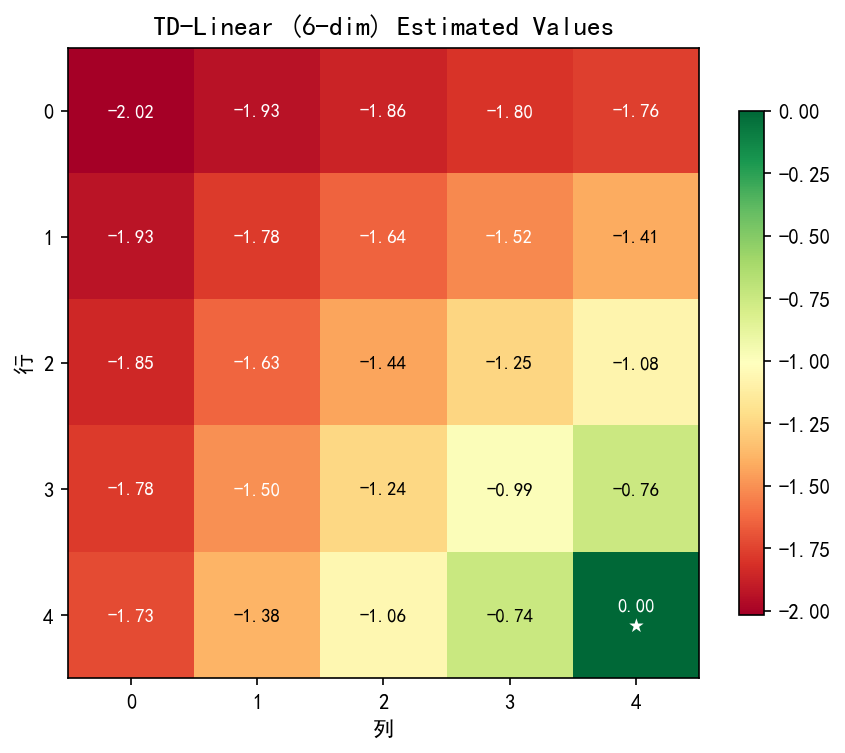
\includegraphics[width=\linewidth]{exp5/results/task1_td_6d_val.png}
\end{minipage}\hfill
\begin{minipage}{0.49\textwidth}
\centering
\textbf{TD-Linear（10维）状态价值估计}\\[0.4em]
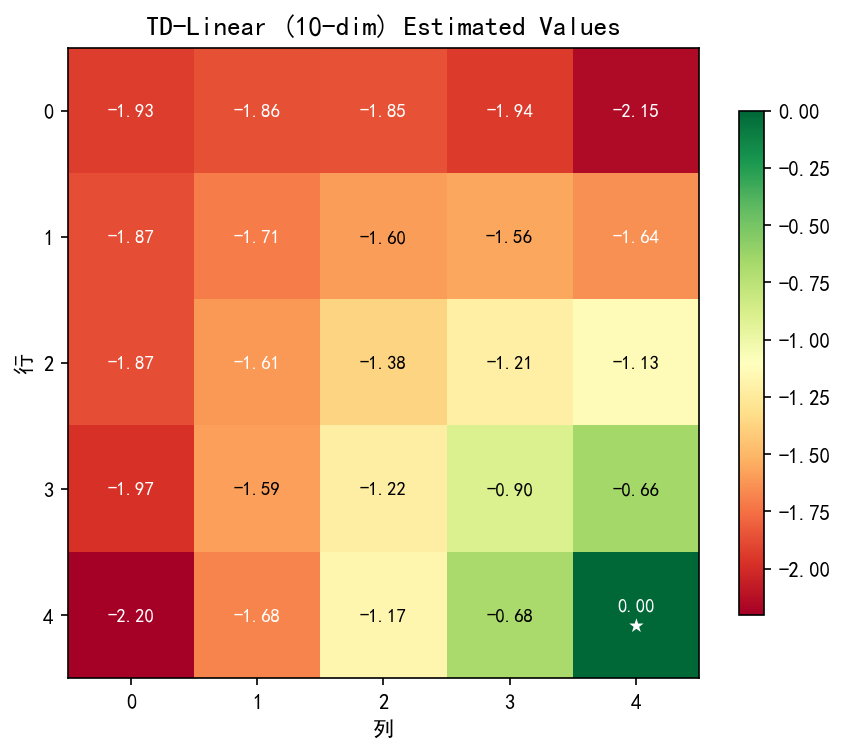
\includegraphics[width=\linewidth]{exp5/results/task1_td_10d_val.png}
\end{minipage}
\caption{不同近似维度与方法下的状态价值估计热力图对比}
\end{figure}

\paragraph{结果分析}
随着特征维数增加，TD-Linear 的最终 RMSE 持续下降，说明高阶特征能够表达更多价值函数形状。10 维近似的 RMSE 为 $0.3843$，已接近 TD-Table 的 $0.3141$，但仍存在由特征空间限制带来的近似误差。

\paragraph{思考题}



\question{问题：为什么线性近似无法精确拟合真实状态值？如何改善？}

\answerlabel 线性近似只能在给定特征张成的函数空间内寻找解。使用 3 维特征
\[
\phi(s)=[1,x,y]^\top
\]
时，$\hat v(s,\mathbf w)=\phi(s)^\top\mathbf w$ 只能表示关于坐标的一阶平面；而基准价值在目标附近变化较快，整体也不是一阶平面，因此会产生不可消除的近似偏差。

实验结果体现了这一限制：特征维数由 3 维增加到 6 维和 10 维后，最终 RMSE 从 $0.9892$ 降至 $0.5867$ 和 $0.3843$，说明高阶特征提高了表达能力；但 10 维线性近似的误差仍高于 TD-Table 的 $0.3141$，表明全局多项式特征仍无法完全表示该价值函数。

可从两个方向改善。其一是设计更适合任务结构的特征，例如加入到目标的距离或使用 Tile Coding，使局部区域可以相对独立地调整；其二是使用能够表示非线性关系的模型。无论采用哪种方法，都应通过独立误差指标检查是否真正降低了近似偏差。


\subsubsection{任务 2：基于线性函数近似的 Sarsa 算法}

线性函数近似 Sarsa 将动作价值函数近似为 $\hat{q}(s,a,\mathbf{w}) = \mathbf{w}^\top \mathbf{x}(s,a)$，结合 $\varepsilon$-greedy 探索和半梯度 Sarsa 更新 $\mathbf{w} \leftarrow \mathbf{w} + \alpha \delta_t \mathbf{x}(S_t, A_t)$（其中 $\delta_t$ 为 TD 误差），在线学习控制策略。函数近似引入了参数共享，使得对某 $(s,a)$ 的更新会通过特征向量泛化影响所有相似状态-动作对的估计。

\paragraph{实验设置}
在控制任务中，状态--动作特征定义为
\[
\phi(s,a)=\operatorname{one\text{-}hot}(a)\otimes\phi(s),
\]
并使用线性函数
\[
\hat q(s,a,\mathbf w)=\phi(s,a)^\top\mathbf w
\]
近似动作价值。动作选择采用 $\epsilon$-greedy 策略，其中 $\epsilon=0.1$。

\paragraph{策略演变、收敛曲线及最终策略}

\begin{figure}[H]
\centering
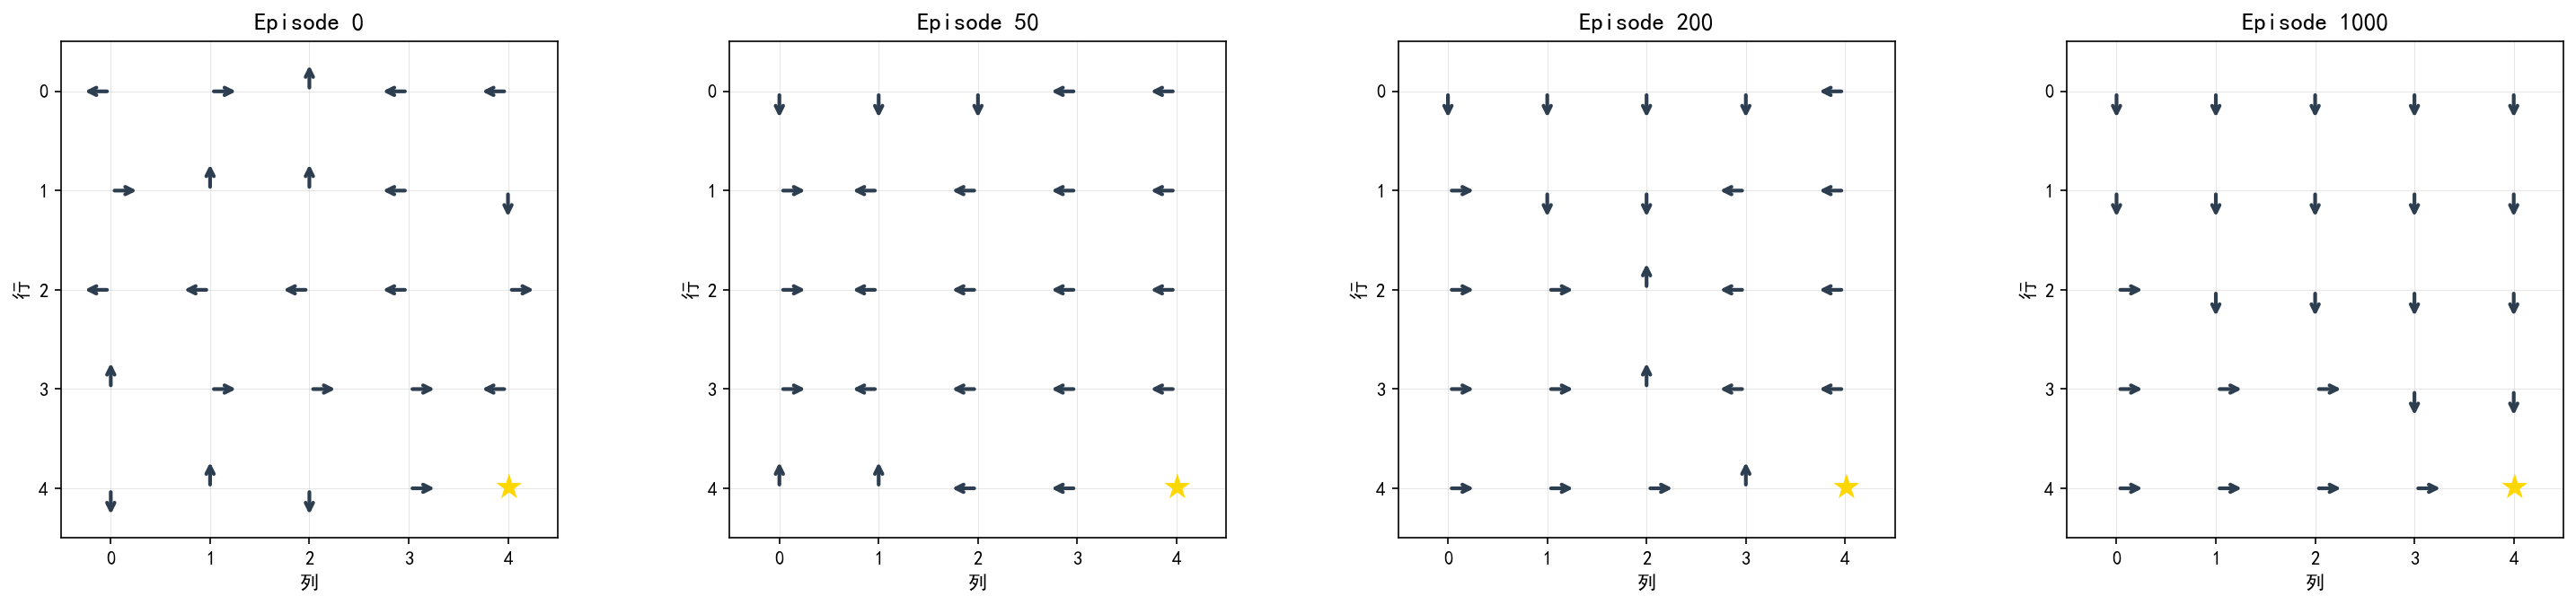
\includegraphics[width=\textwidth]{exp5/results/task2_sarsa_policy_evolution.png}
\caption{函数近似 Sarsa 在不同训练阶段的贪心策略}
\end{figure}

训练前各动作价值相同，图中的初始箭头由并列动作中随机选取；训练至第 50 和第 200 回合时，部分状态仍存在绕行或方向不一致；第 1000 回合时，各非终止状态已形成可到达目标的路径。该过程图与奖励、成功率曲线共同说明策略逐步稳定，而非仅展示最终结果。

\begin{figure}[H]
\centering
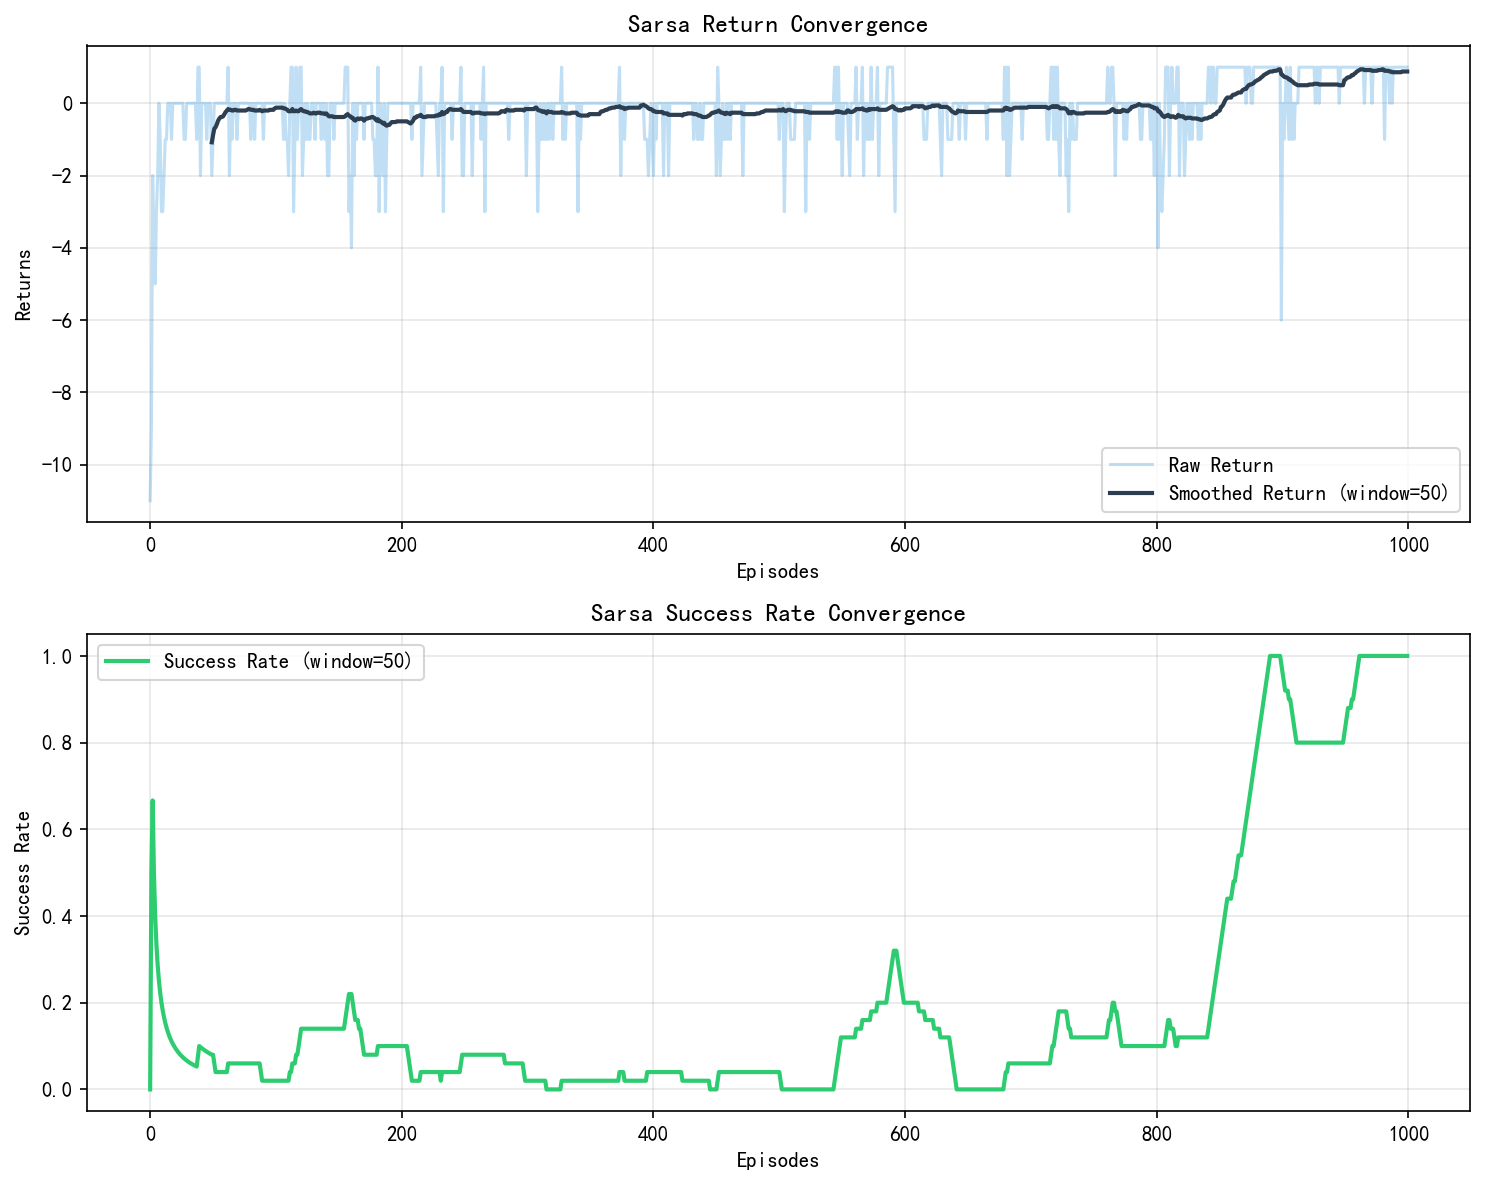
\includegraphics[width=0.75\textwidth]{exp5/results/task2_sarsa_convergence.png}
\caption{Sarsa 收敛曲线}
\end{figure}
\begin{figure}[H]
\centering
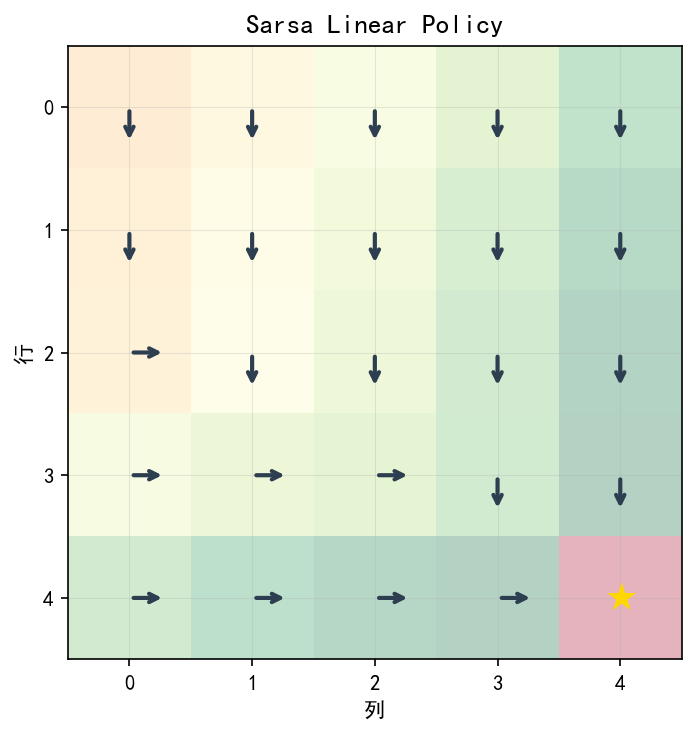
\includegraphics[width=0.5\textwidth]{exp5/results/task2_sarsa_policy.png}
\caption{Sarsa 最终策略}
\end{figure}

\paragraph{结果分析}
在 $\alpha=0.01$ 时，训练结束后的成功率为 $0.00\%$；将学习率调整为 $\alpha=0.05$ 后，成功率达到 $100\%$，平均路径长度为 4.17 步。结合策略演变图可见，训练中间阶段仍存在绕行或方向不一致，至第 1000 回合时策略才基本稳定。该结果说明当前特征尺度下学习率对参数共享更新的影响明显，但不能据此认定更大的学习率普遍更优。

\paragraph{思考题}



\question{问题：函数近似的 Sarsa 与表格型 Sarsa 在更新方式上有何不同？}

\answerlabel 表格型 Sarsa 直接更新当前状态--动作对对应的单元：
\[
Q(S_t,A_t)\leftarrow Q(S_t,A_t)+\alpha\delta_t.
\]
其他状态--动作对的数值不会因此改变，因此更新是局部的。

线性函数近似 Sarsa 更新共享参数：
\[
\mathbf w\leftarrow \mathbf w+\alpha\delta_t\phi(S_t,A_t).
\]
由于多个状态--动作对可能使用相同参数或相似特征，一次更新也会改变它们的估计值。这种参数共享能够把已访问状态的信息推广到相似状态，但也可能产生参数干扰。

本实验中，$\alpha=0.01$ 与 $\alpha=0.05$ 得到了不同训练结果，说明函数近似下的学习率会同时影响一组相关估计，不能直接按表格型算法的局部更新方式理解。


\subsubsection{任务 3：基于线性函数近似的 Q-learning 算法}

线性函数近似 Q-learning 使用异策略更新：行为策略 $\varepsilon$-greedy 负责探索，TD 目标始终采用 $\max_{a'} \hat{q}(S', a', \mathbf{w})$（贪心目标策略）。在函数近似下，Q-learning 面临``死亡三要素''（Deadly Triad）——函数近似 $\times$ 自举 $\times$ 异策略——理论上可能发散，实验中可能出现比 Sarsa 更不稳定的现象。

在相同环境下运行线性近似 Q-learning 算法（在线版本使用 $\alpha=0.05, \epsilon=0.1$），并与 Sarsa 进行对比。

\paragraph{结果数据}
\begin{itemize}
\item \textbf{Sarsa 在线评估}：成功率 = 100.00\%，平均路径长度 = 4.17 步。
\item \textbf{Q-learning 在线评估}：成功率 = 100.00\%，平均路径长度 = 4.17 步。
\end{itemize}

\paragraph{收敛曲线及最终策略}

\begin{figure}[H]
\centering
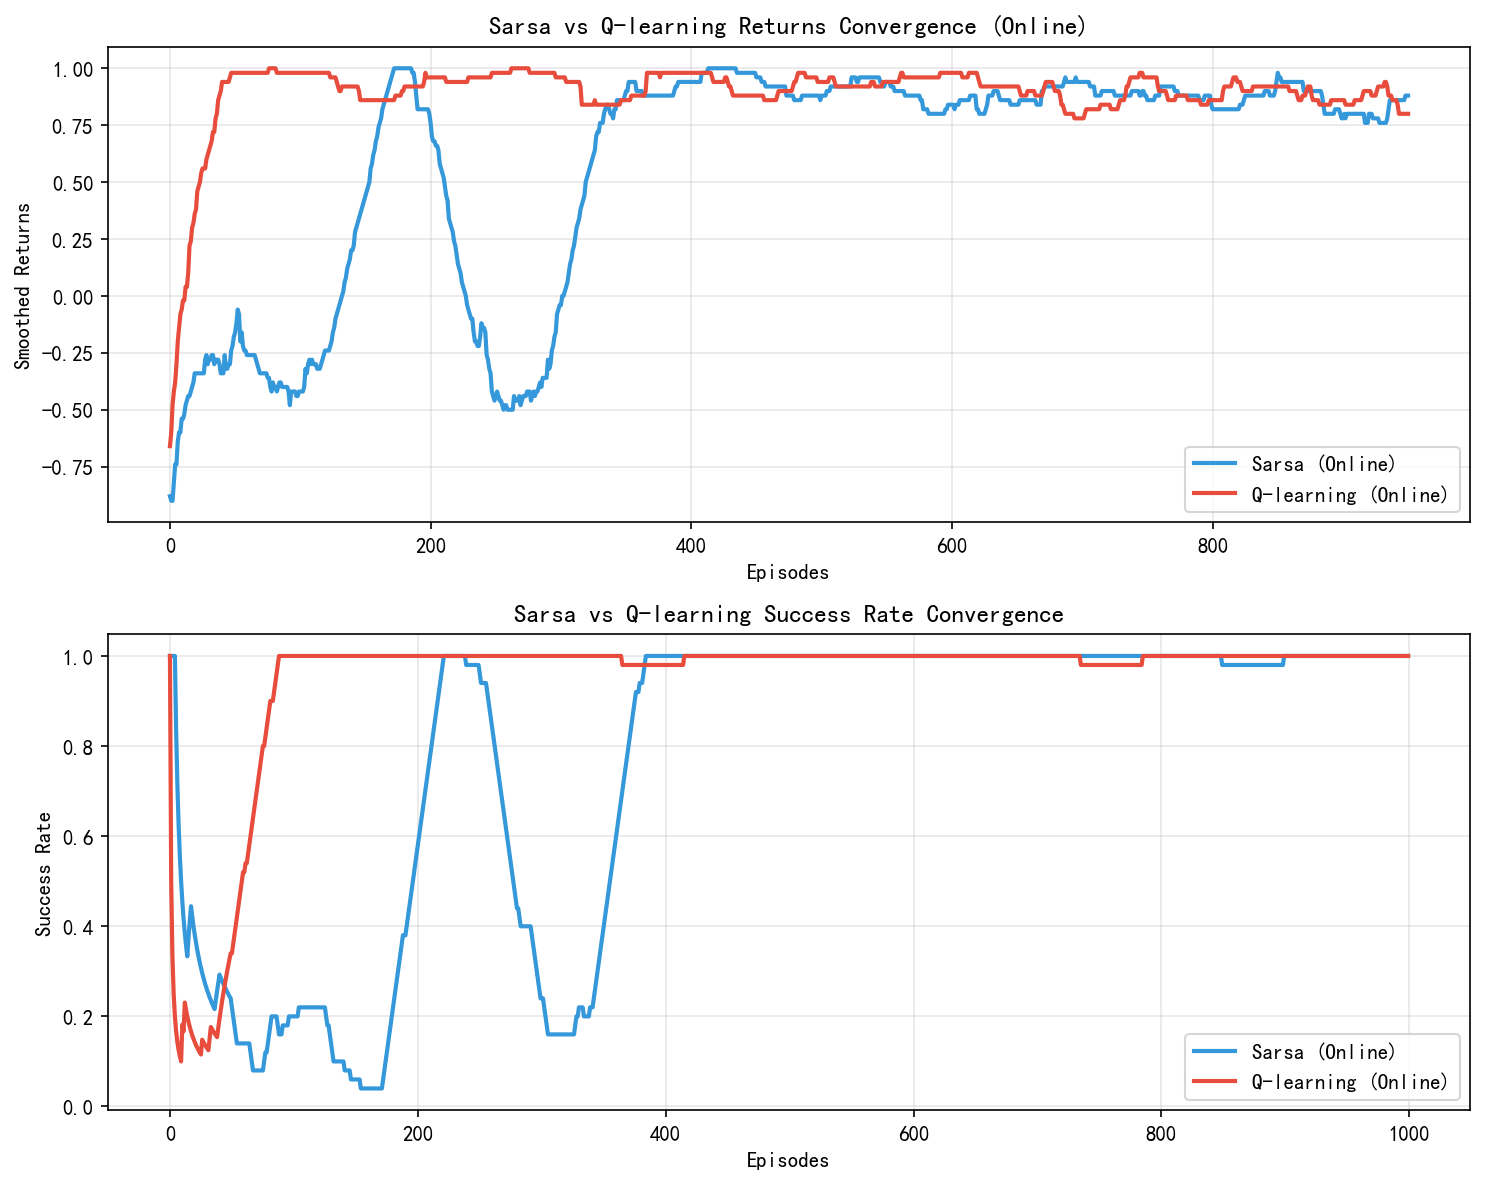
\includegraphics[width=0.75\textwidth]{exp5/results/task3_sarsa_vs_q_convergence.png}
\caption{Q-learning vs Sarsa 收敛对比}
\end{figure}
\begin{figure}[H]
\centering
\begin{minipage}{0.49\textwidth}
\centering
\textbf{Sarsa 最终策略}\\[0.4em]
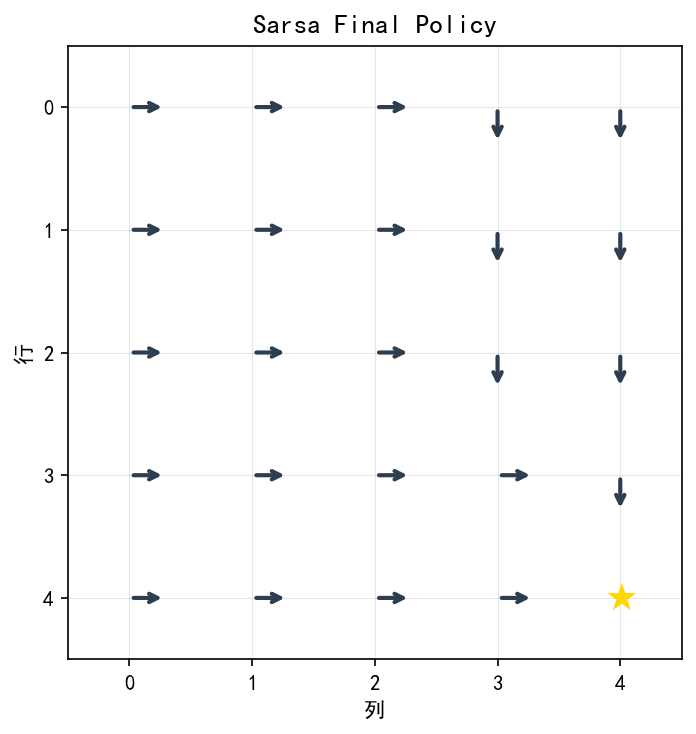
\includegraphics[width=0.82\linewidth]{exp5/results/task3_sarsa_policy.png}
\end{minipage}\hfill
\begin{minipage}{0.49\textwidth}
\centering
\textbf{Q-learning 最终策略}\\[0.4em]
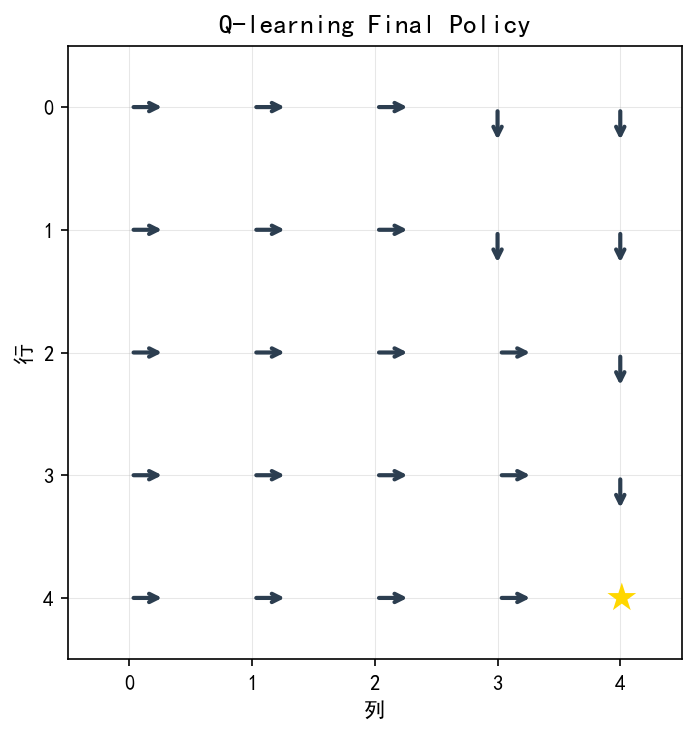
\includegraphics[width=0.82\linewidth]{exp5/results/task3_q_policy.png}
\end{minipage}
\caption{线性函数近似 Sarsa 与 Q-learning 的最终策略}
\end{figure}

\paragraph{结果分析}
两种算法最终均达到 $100\%$ 成功率和 4.17 步平均路径长度，曲线未显示明显发散。当前确定性小规模 GridWorld 和所用特征不足以触发显著稳定性差异，因此这里只能确认两种算法在本次设置下均完成了控制学习。

\paragraph{思考题}



\question{问题 1：为什么 Q-learning 是异策略算法？在函数近似下，这一特性带来了什么优势？}

\answerlabel Q-learning 可以使用 $\epsilon$-greedy 行为策略生成转移样本，但其 TD 目标为
\[
R_{t+1}+\gamma\max_{a'}\hat q(S_{t+1},a',\mathbf w),
\]
对应的是贪心目标策略。行为策略与目标策略不同，因此 Q-learning 属于异策略算法。

这种分离使行为策略能够持续探索，而参数更新仍朝向贪心目标策略。在函数近似下，一次更新还会通过共享参数影响相似状态--动作对，因此有限的探索样本可以传播到未充分访问的区域。与此同时，这种组合也引入了稳定性风险，不能只将其视为优势。


\question{问题 2：在实验中发现 Q-learning 是否比 Sarsa 更容易发散？为什么？}

\answerlabel 本次实验中，两种算法均达到 $100\%$ 成功率和 4.17 步平均路径长度，收敛曲线也未显示 Q-learning 明显发散。因此，从当前数据不能得出 Q-learning 比 Sarsa 更容易发散的实验结论。

理论上，Q-learning 同时使用函数近似、自举和异策略更新，缺少一般性的收敛保证；最大值目标还可能放大估计误差。该风险说明它在某些特征、步长或环境下可能不稳定，但并不意味着每次小规模实验都会出现发散。本实验结论仅适用于当前设置。


\subsubsection{任务 4：深度 Q-learning（DQN）初步}

DQN（Deep Q-Network）将 Q 函数用深度神经网络近似，并引入两项关键稳定技术：\textbf{经验回放（Experience Replay）}将历史转移 $(s,a,r,s')$ 存入回放缓冲区并随机采样，打破样本时序相关性；\textbf{目标网络（Target Network）}使用延迟更新的副本网络计算 TD 目标，避免追逐快速变动的目标导致训练振荡。

使用单隐藏层神经网络（100个神经元，ReLU激活）逼近动作值函数，并结合经验回放（容量 500，Batch Size 32）与目标网络（每 50 步同步一次）。在 GridWorld 连续在线运行 1000 步，并与表格型 Q-learning（在线运行 1000 步）进行样本效率的对比。

\paragraph{结果数据}
\begin{itemize}
\item \textbf{DQN 最终评估}：成功率 = \textbf{100.00\%}，平均路径长度 = \textbf{4.17 步}。
\item \textbf{Tabular Q-learning 最终评估}：成功率 = \textbf{50.00\%}，平均路径长度 = \textbf{3.17 步}。
\end{itemize}

\paragraph{样本效率对比及网络 Loss 曲线}

\begin{figure}[H]
\centering
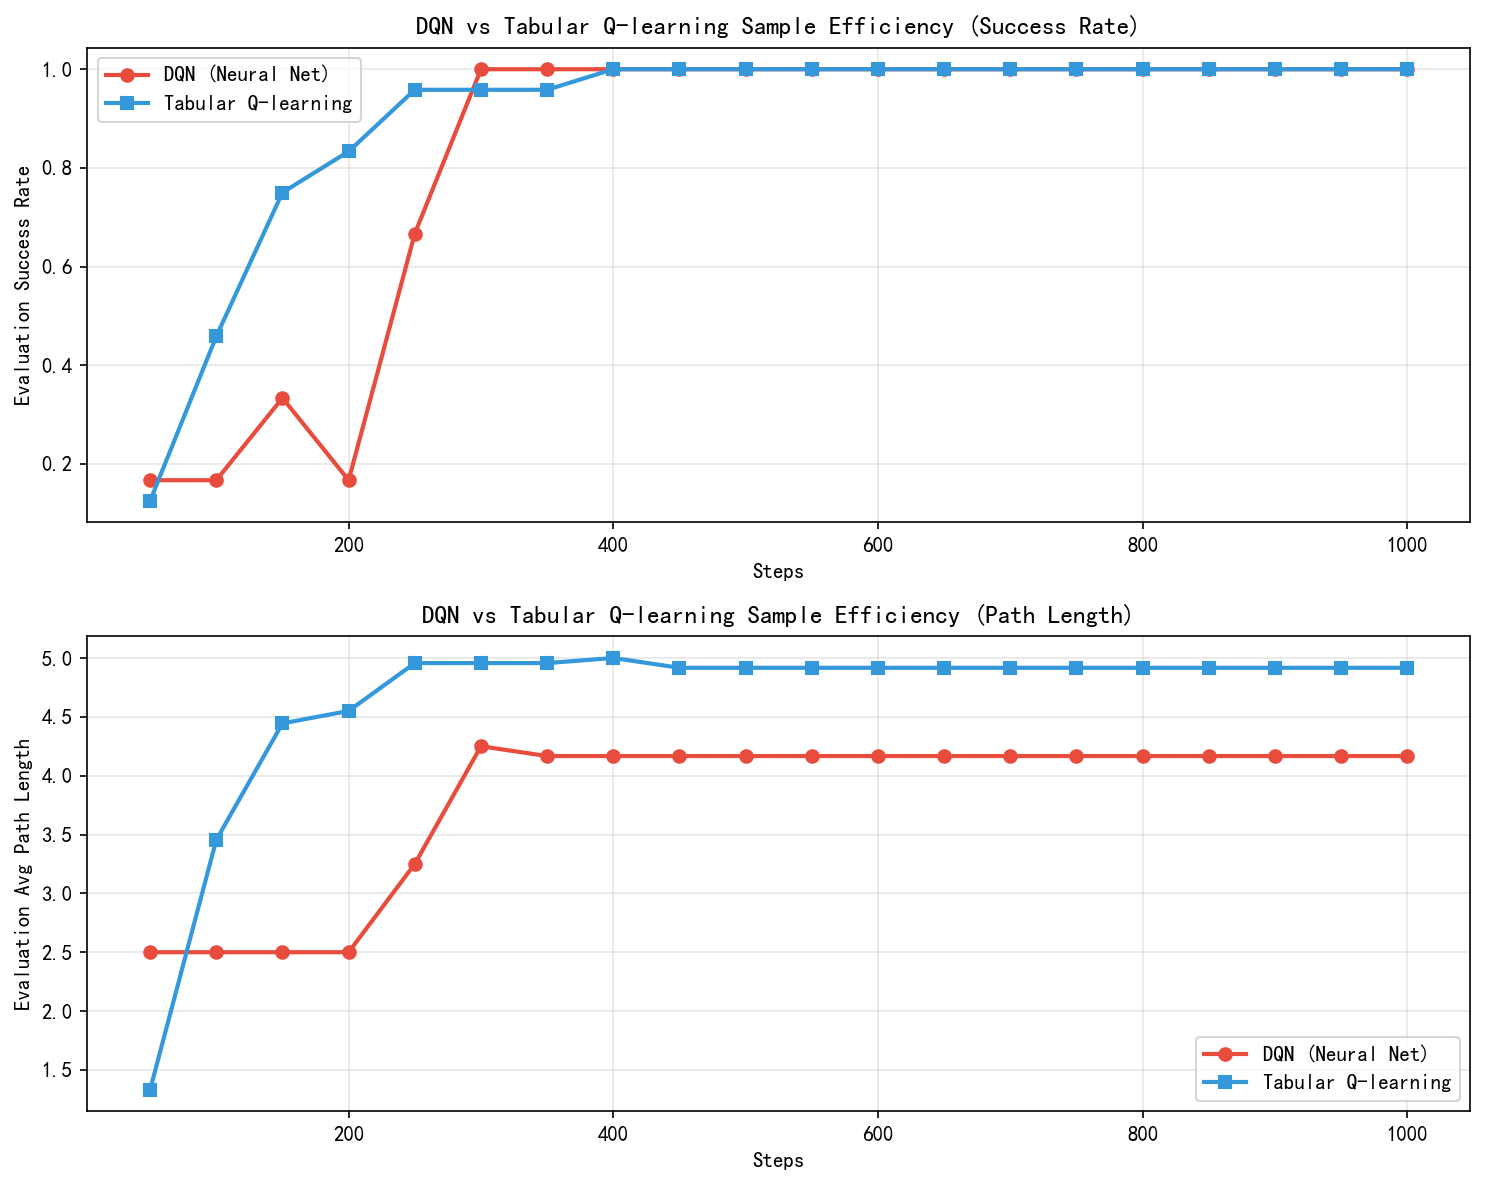
\includegraphics[width=0.75\textwidth]{exp5/results/task4_dqn_vs_tabular.png}
\caption{样本效率对比}
\end{figure}
\begin{figure}[H]
\centering
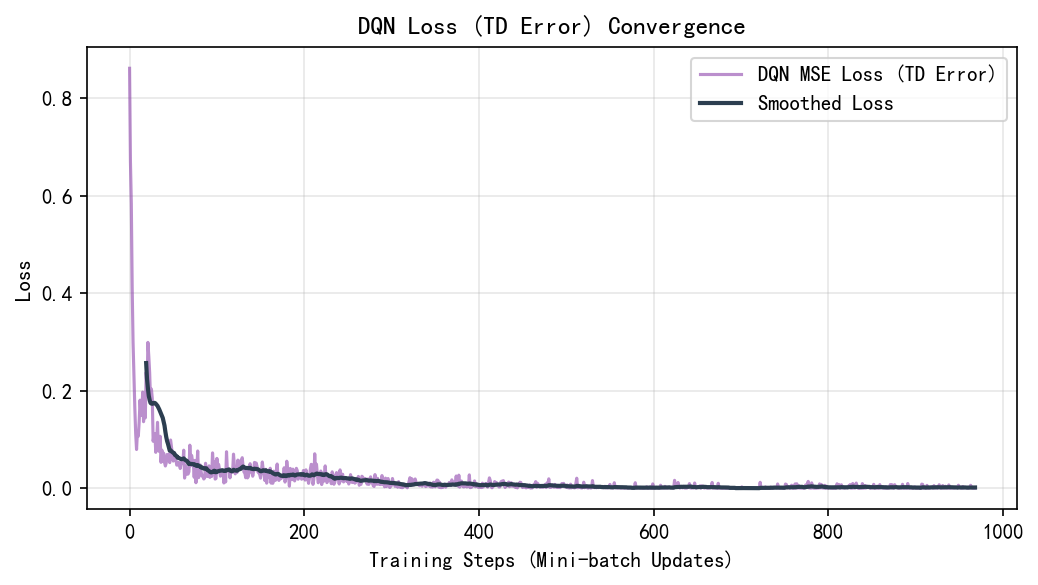
\includegraphics[width=0.75\textwidth]{exp5/results/task4_dqn_loss.png}
\caption{DQN Loss 收敛曲线}
\end{figure}

\begin{figure}[H]
\centering
\begin{minipage}{0.49\textwidth}
\centering
\textbf{DQN 最终策略}\\[0.4em]
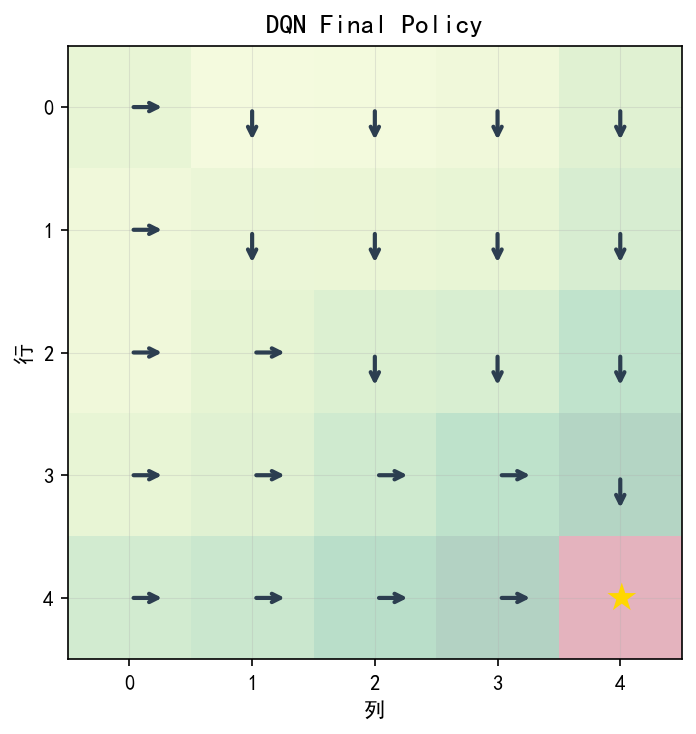
\includegraphics[width=0.9\linewidth]{exp5/results/task4_dqn_policy.png}
\end{minipage}\hfill
\begin{minipage}{0.49\textwidth}
\centering
\textbf{表格型 Q-learning 最终策略}\\[0.4em]
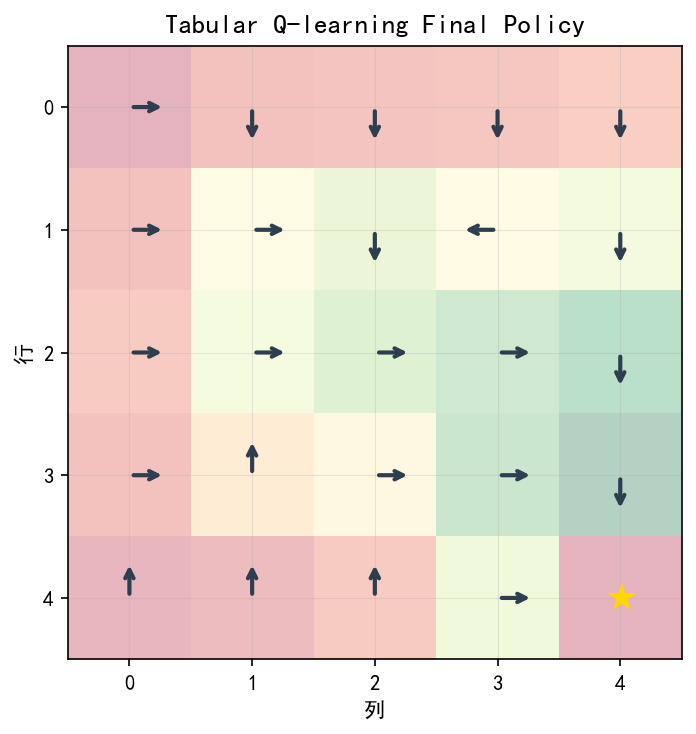
\includegraphics[width=0.9\linewidth]{exp5/results/task4_tabular_policy.png}
\end{minipage}
\caption{DQN 与表格型 Q-learning 的最终策略}
\end{figure}

\paragraph{结果分析}
在相同的 1000 步在线交互预算下，DQN 的最终成功率为 $100\%$，表格型 Q-learning 为 $50\%$。该结果表明参数共享和重复采样在本次设置下有助于更快传播价值信息；由于只比较了单一网络结构和一次实验配置，不能将其推广为 DQN 普遍优于表格方法的结论。表格方法统计出的 3.17 步平均路径只覆盖成功回合，需与其 $50\%$ 成功率同时解读。

\paragraph{思考题}



\question{问题：经验回放和目标网络分别解决了什么问题？}

\answerlabel 经验回放将在线交互得到的转移存入缓冲区，并随机抽取小批量样本训练。它主要减弱连续转移之间的时间相关性，同时允许同一条经验被重复使用，从而提高已有交互数据的利用率。随机采样只能减弱相关性，并不能使样本严格独立同分布。

目标网络使用延迟更新的参数 $\mathbf w^-$ 计算 TD 目标：
\[
y=r+\gamma\max_{a'}Q(s',a';\mathbf w^-).
\]
在若干训练步内保持 $\mathbf w^-$ 不变，可以减缓“预测网络更新时目标也同时变化”的问题，使回归目标相对稳定。目标网络降低了振荡风险，但不能单独保证 DQN 一定收敛。

\subsection{核心代码与分析}

\subsubsection{TD-Linear 参数更新}
在 \texttt{task1\_td\_linear.py} 中，TD-Linear 核心迭代更新实现如下：
\begin{lstlisting}[language=python]
# 获取当前状态与下一状态的特征
phi_s = get_features(s, env, dim)
val_s = np.dot(phi_s, w)

if env.is_terminal(s_next):
    val_next = 0.0
else:
    phi_next = get_features(s_next, env, dim)
    val_next = np.dot(phi_next, w)

# 计算 TD 目标与 TD 误差
td_target = reward + env.gamma * val_next
td_error = td_target - val_s

# 根据半梯度下降更新权重参数
w += alpha * td_error * phi_s
\end{lstlisting}

该实现直接对应线性半梯度 TD 更新。计算梯度时只对当前状态估计 $\hat v(s,\mathbf w)$ 求导，并将下一状态估计视为固定目标，因此称为半梯度方法。

\subsubsection{Sarsa 联合特征计算与更新}
在 \texttt{task2\_sarsa.py} 中，状态-动作特征使用 Kronecker 积形式的独热拼接表示：
\begin{lstlisting}[language=python]
def get_joint_features(s, a, env, state_dim=6):
    row, col = env.state_to_pos(s)
    # 状态坐标归一化
    x = (col + 1.0) / 5.0
    y = (row + 1.0) / 5.0
    if state_dim == 6:
        phi_s = np.array([1.0, x, y, x**2, y**2, x*y])
    
    # 状态特征与动作独热拼接 (维度为 state_dim * 4)
    phi = np.zeros(state_dim * env.num_actions)
    phi[a * state_dim : (a + 1) * state_dim] = phi_s
    return phi
\end{lstlisting}

该实现为每个动作分配独立的参数块，并在对应参数块中写入状态特征。因此不同动作的权重彼此分离，同一动作下的相似状态则通过共享状态特征产生泛化。

\subsubsection{DQN 经验回放与目标网络更新}
在 \texttt{task4\_dqn.py} 中，模型对目标网络和回放缓冲区的组合优化如下：
\begin{lstlisting}[language=python]
# 从经验回放中随机采样一个 Batch
states_b, actions_b, rewards_b, next_states_b, dones_b = replay_buffer.sample(batch_size)

states_t = torch.tensor(states_b)
actions_t = torch.tensor(actions_b).unsqueeze(1)
rewards_t = torch.tensor(rewards_b)
next_states_t = torch.tensor(next_states_b)
dones_t = torch.tensor(dones_b)

# 预测当前动作价值 Q(s, a)
current_q = q_net(states_t).gather(1, actions_t).squeeze(1)

# 使用目标网络计算下一个状态的最大动作价值 max Q(s', a'; w^-)
with torch.no_grad():
    max_next_q = target_net(next_states_t).max(1)[0]
    target_q = rewards_t + env.gamma * max_next_q * (1.0 - dones_t)

# 计算 MSE 损失并反向传播
loss = loss_fn(current_q, target_q)
optimizer.zero_grad()
loss.backward()
optimizer.step()
\end{lstlisting}

\texttt{current\_q} 由在线网络计算，\texttt{max\_next\_q} 由目标网络计算，并每隔 50 步同步参数；训练样本从回放缓冲区随机抽取。两种机制分别减缓训练目标快速变化和连续样本相关性带来的影响。
\subsection{总结与体会}
本实验比较了表格型表示与值函数近似方法在策略评估和控制任务中的表现。
\begin{enumerate}
\item 在\textbf{策略评估}中，3 维、6 维和 10 维线性特征的最终 RMSE 依次下降，说明增加有效特征能够减小近似偏差；目标附近的离散价值变化仍限制了平滑函数的拟合精度。
\item 在\textbf{控制任务}中，同一组参数会同时影响多个状态，带来表格方法中不存在的跨状态干扰。因此学习率和特征尺度需要结合训练曲线调节，不能直接沿用表格算法设置。
\item 在 1000 步对比实验中，DQN 的成功率为 $100\%$，表格 Q-learning 为 $50\%$。该结果说明在本次网络结构和数据设置下，参数共享有助于传播价值信息；单次小规模实验不足以证明 DQN 在一般情形下必然具有更高样本效率。
\end{enumerate}

\newpage
\section{策略函数近似}

\subsection{实验目的与要求}

\begin{enumerate}
\item 理解从值函数方法到策略梯度方法的转变：掌握策略参数化的基本思想及其与表格策略的区别。
\item 掌握策略梯度方法的核心原理：理解最优策略指标（平均状态价值）的定义及其梯度表达式。
\item 实现REINFORCE算法：能够使用蒙特卡洛采样估计动作价值，并完成策略参数的梯度上升更新。
\item 理解Softmax策略参数化：掌握如何用Softmax函数保证策略的随机性和探索性。
\end{enumerate}
\subsection{实验内容与设计}

\subsubsection{公共环境与策略表示}

实验使用 $5\times5$ GridWorld、折扣因子 $\gamma=0.9$ 和状态特征 $\phi(s)=[1,x,y]^\top$。每个动作维护独立偏好参数，经过 Softmax 转换为动作概率。评价指标包括回合总奖励、最终贪心策略和指定状态下各动作概率的变化。

\subsubsection{任务 1：参数化策略设计}

固定随机种子初始化参数，展示中间状态和全局初始动作概率。通过 Softmax 表达式分析所有动作概率严格为正的原因，并检查数值稳定化处理是否保持概率归一化。

\subsubsection{任务 2：REINFORCE 实验设计}

每个 episode 按当前策略生成完整轨迹，从后向前计算折扣回报，并按任务书公式使用 $\gamma^tG_t$ 加权对数策略梯度。训练设置为学习率 $0.001$、最多 500 步和 1000 个 episode；记录总奖励曲线、最终策略和起点动作概率。

\subsubsection{任务 3：探索与利用分析设计}

训练期间持续记录起点状态四个动作的概率。结合回报符号和动作当前概率分析更新方向，观察高回报动作概率是否增加，以及 Softmax 策略在训练后是否仍保留非零探索概率。




\subsection{实验过程、结果与分析}

\subsubsection{任务 1：策略的参数化表示}

策略的参数化表示（Policy Parameterization）用 Softmax 函数将特征偏好（preference）转化为概率分布：$\pi(a|s,\boldsymbol{\theta}) = \frac{\exp(h(s,a,\boldsymbol{\theta}))}{\sum_{a'}\exp(h(s,a',\boldsymbol{\theta}))}$，其中 $h(s,a,\boldsymbol{\theta}) = \boldsymbol{\theta}^\top \mathbf{x}(s,a)$。Softmax 保证所有动作概率严格大于零，天然支持持续探索，策略对参数 $\boldsymbol{\theta}$ 可微，是策略梯度方法的基础。

\paragraph{实验设置与特征设计}
我们在 $5 \times 5$ 网格世界中实现了一个 Softmax 参数化随机策略。
\begin{itemize}
\item \textbf{状态空间}：共 25 个状态。坐标表示为 $(x, y) \in \{1, 2, 3, 4, 5\}$，其中 $x$ 为行坐标，$y$ 为列坐标。
\item \textbf{动作空间}：上（0）、下（1）、左（2）、右（3）共 4 个方向。
\item \textbf{折扣因子}：$\gamma = 0.9$。
\item \textbf{特征表示}：使用线性特征表示，对于状态 $s$，定义特征向量为：
  $$\phi(s) = [1, x, y]^T$$
  其中 $x = \text{row} + 1$，$y = \text{col} + 1$。
\item \textbf{偏好函数与 Softmax 策略}：
  对每个动作 $a \in \{0, 1, 2, 3\}$，定义其偏好函数为：
  $$h(s, a, \theta) = \phi(s)^T \theta_a$$
  其中 $\theta_a \in \mathbb{R}^3$ 是动作 $a$ 对应的参数向量。四个动作 of parameters 构成大小为 $4 \times 3$ 的矩阵 $\theta$。
  动作选择概率通过 Softmax 函数计算：
  $$\pi(a|s, \theta) = \frac{e^{h(s, a, \theta)}}{\sum_{b=0}^{3} e^{h(s, b, \theta)}}$$
\end{itemize}

\paragraph{初始策略分布可视化}
固定随机种子（\texttt{seed=42}），随机初始化参数 $\theta \sim N(0, 0.1)$。
\begin{itemize}
\item \textbf{特定状态 (3,3) 的初始概率分布} 如下图所示：
\begin{figure}[H]
\centering
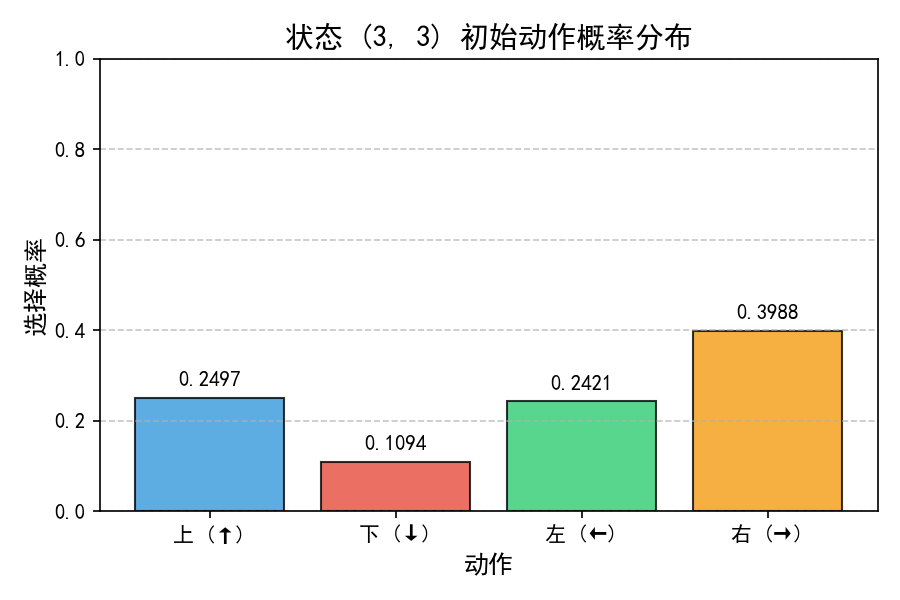
\includegraphics[width=0.75\textwidth]{exp6/results/task1_state_33_probs.png}
\caption{状态 (3,3) 初始动作概率分布}
\end{figure}
\end{itemize}

\begin{itemize}
\item \textbf{初始整体策略概率分布} 如下图所示（箭头的方向和粗细/透明度代表各动作的选择概率）：
\begin{figure}[H]
\centering
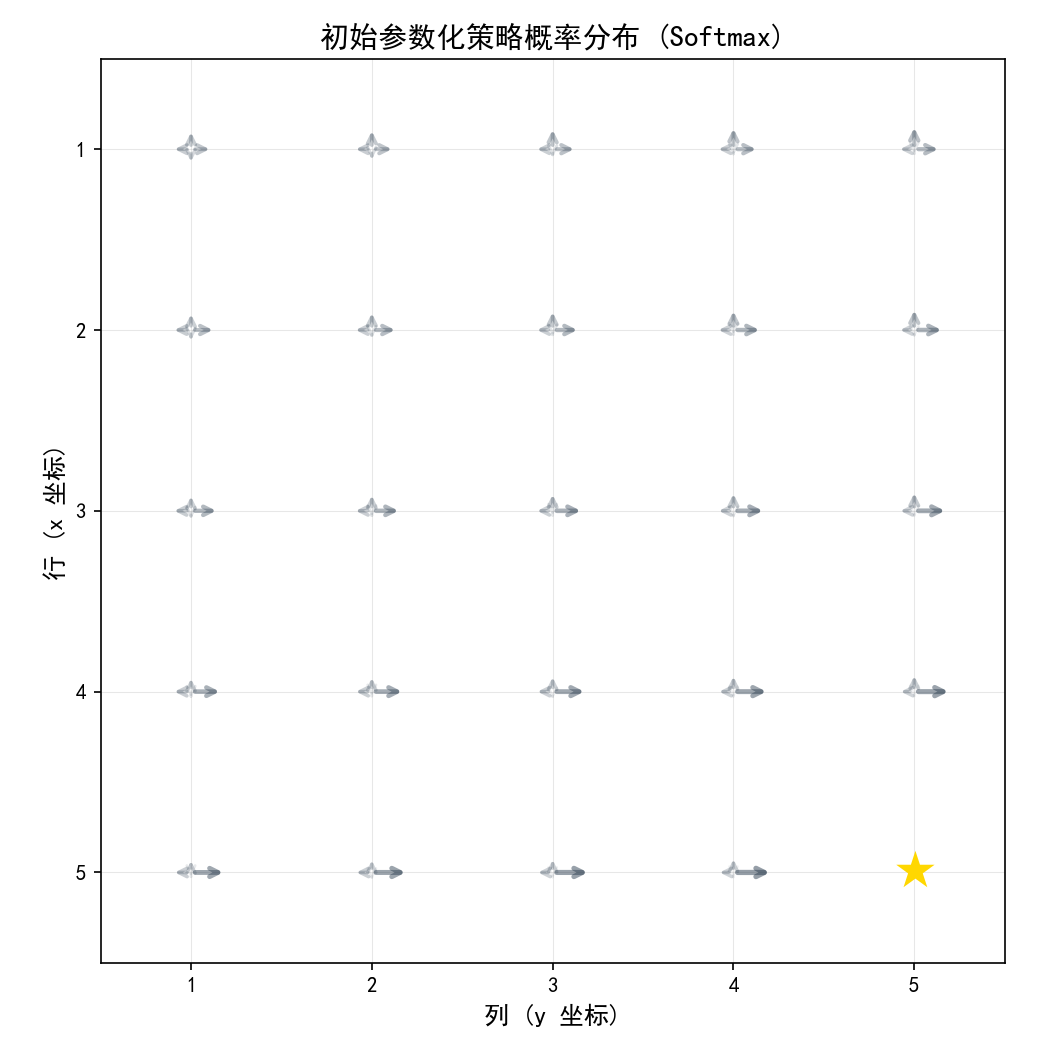
\includegraphics[width=0.5\textwidth]{exp6/results/task1_initial_policy.png}
\caption{初始参数化策略概率分布}
\end{figure}
\end{itemize}

\paragraph{思考题}


\question{问题：Softmax 函数如何保证 $\pi(a|s,\theta)>0$？这对探索有何意义？}

\answerlabel Softmax 策略为
\[
\pi(a|s,\theta)=
\frac{\exp(h(s,a,\theta))}
{\sum_b\exp(h(s,b,\theta))}.
\]
当偏好值 $h(s,a,\theta)$ 有限时，指数项严格为正，分母也是若干正数之和，因此每个动作的概率都严格大于零。

这意味着训练期间非贪心动作仍有机会被采样，不会像确定性贪心策略那样直接把某些动作排除。但概率可以变得非常小，所以“概率非零”只保证理论上的可采样性，并不保证有限训练过程中能充分探索所有动作。


\subsubsection{任务 2：REINFORCE 算法实现}

REINFORCE 算法是基于策略梯度定理（Policy Gradient Theorem）的 Monte Carlo 策略优化方法：$\boldsymbol{\theta} \leftarrow \boldsymbol{\theta} + \alpha \gamma^t G_t \nabla_{\boldsymbol{\theta}} \ln \pi(A_t|S_t,\boldsymbol{\theta})$。它使用每条完整 episode 的实际累积回报 $G_t$ 作为梯度方向的权重，正回报增加该动作概率，负回报减少，是同策略（On-policy）算法，无需环境模型。

\paragraph{算法更新公式与推导}
REINFORCE 算法是通过随机梯度上升最大化目标 $J(\theta)$ 的算法。其目标函数是回合的期望折扣累积回报：
$$\nabla_\theta J(\theta) = \mathbb{E}_{\pi} \left[ q_t(s_t, a_t) \nabla_\theta \ln \pi(a_t|s_t, \theta) \right]$$
因此，对数似然梯度的更新公式为：
$$\theta_a \leftarrow \theta_a + \alpha q_t(s_t, a_t) \nabla_{\theta_a} \ln \pi(a_t|s_t, \theta)$$
对对数似然项求导：
$$\ln \pi(a_t|s_t, \theta) = \phi(s_t)^T \theta_{a_t} - \ln \sum_b e^{\phi(s_t)^T \theta_b}$$
对特定动作参数向量 $\theta_{a'}$ 求偏导：
$$\nabla_{\theta_{a'}} \ln \pi(a_t|s_t, \theta) = \phi(s_t) \left( \mathbb{I}(a' = a_t) - \pi(a'|s_t, \theta) \right)$$
其中 $\mathbb{I}$ 为指示函数。因此，REINFORCE 的具体更新规则为：
$$\theta_{a'} \leftarrow \theta_{a'} + \alpha q_t(s_t, a_t) \phi(s_t) \left( \mathbb{I}(a' = a_t) - \pi(a'|s_t, \theta) \right)$$


\paragraph{实验超参数设置}
\begin{itemize}
\item \textbf{学习率} $\alpha = 0.001$
\item \textbf{单回合最大步数} $T_{\text{max}} = 500$
\item \textbf{训练回合数} $\text{episodes} = 1000$
\item \textbf{折扣因子} $\gamma = 0.9$
\end{itemize}

\paragraph{实验结果}
收敛曲线同时展示原始单回合总奖励和 50 回合滑动平均值：
\begin{figure}[H]
\centering
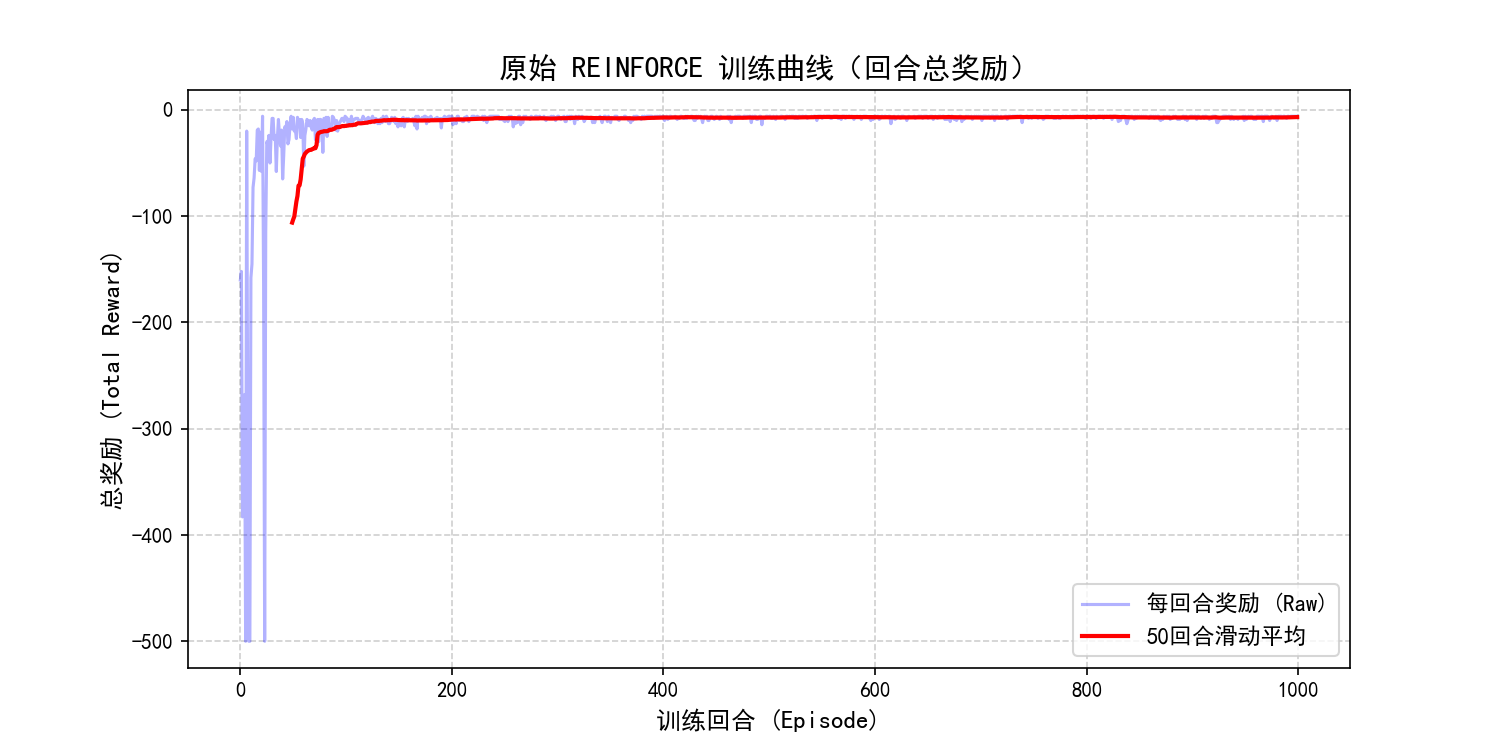
\includegraphics[width=0.75\textwidth]{exp6/results/task2_reward_curve.png}
\caption{REINFORCE 训练收敛曲线}
\end{figure}

\begin{figure}[H]
\centering
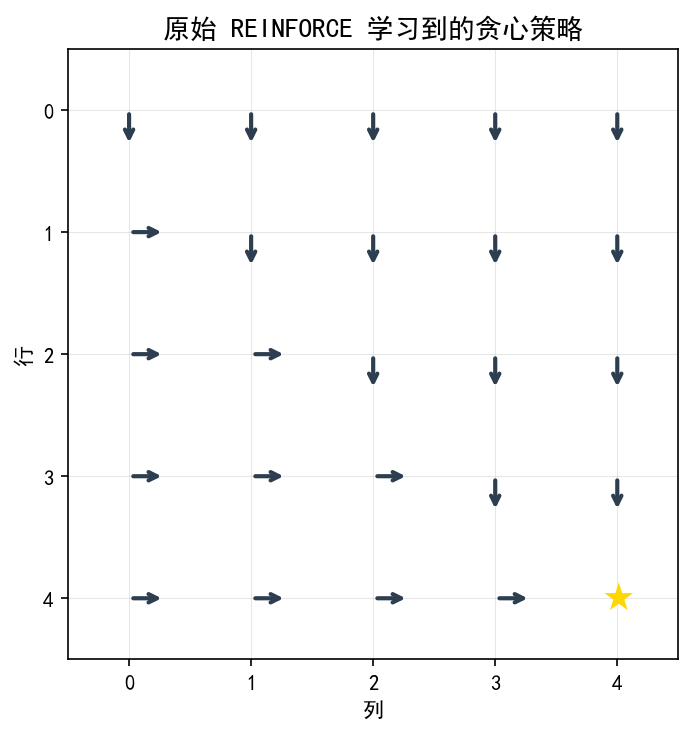
\includegraphics[width=0.45\textwidth]{exp6/results/task2_final_greedy_policy.png}
\caption{REINFORCE 学习到的贪心策略}
\end{figure}

\begin{figure}[H]
\centering
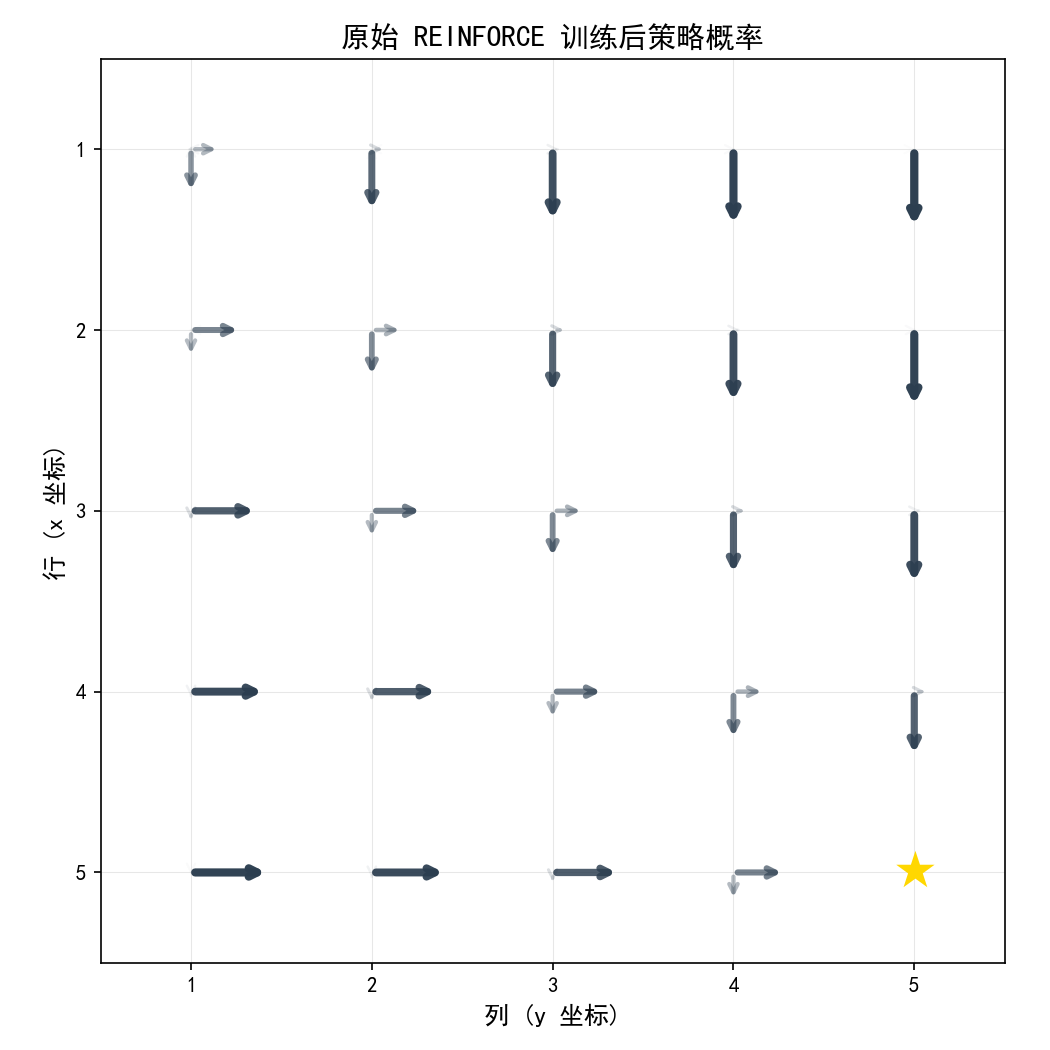
\includegraphics[width=0.45\textwidth]{exp6/results/task2_final_policy_probs.png}
\caption{训练后参数化策略概率分布}
\end{figure}

\paragraph{结果分析}
REINFORCE 前 100 回合平均奖励为 $-60.56$，最后 100 回合平均奖励提高至 $-7.02$，最终回合以 8 步到达目标。训练后的贪心动作总体指向右下角目标，而 Softmax 策略仍为非贪心动作保留非零概率。

\paragraph{思考题}


\question{问题 1：REINFORCE 是同策略算法还是异策略算法？为什么？}

\answerlabel REINFORCE 是同策略（On-policy）算法。
根据策略梯度定理，策略梯度表达式的数学期望为：
$$\nabla_\theta J(\theta) = \mathbb{E}_{S \sim d^{\pi}, A \sim \pi} \left[ q_{\pi}(S, A) \nabla_\theta \ln \pi(A|S, \theta) \right]$$
该期望中的状态分布 $d^{\pi}$ 和动作分布 $\pi$ 都是基于\textbf{当前策略 $\pi_\theta$} 产生的。REINFORCE 算法在更新参数时，必须使用当前策略 $\pi_\theta$ 与环境交互采样得到的回合轨迹（包括状态、动作及其实际回报）来估计期望梯度。如果轨迹是由其他行为策略产生的，该期望估计值将是有偏的，无法代表当前策略梯度。因此它属于同策略算法。

\question{问题 2：REINFORCE 中为什么使用累积回报 $q_t$ 而不是即时奖励？}

\answerlabel 策略梯度的优化目标是长期期望回报，而某个动作的影响可能在若干步之后才体现。REINFORCE 使用
\[
q_t=\sum_{k=t}^{T-1}\gamma^{k-t}r_{k+1}
\]
作为 $q_\pi(s_t,a_t)$ 的 Monte Carlo 样本，使当前动作能够根据其后续结果获得评价。若只使用即时奖励 $r_{t+1}$，当前没有直接奖励但对最终到达目标必要的动作将得不到正确的长期信用分配。

\question{问题 3：该算法与基于值函数的方法（如 Q-learning）在更新方式上有何本质区别？}

\answerlabel REINFORCE 直接参数化策略，并使用完整回合的累计回报更新策略参数；它不进行自举，更新目标方差较大，但可以直接表示随机策略。

Q-learning 学习动作价值函数，并使用单步目标
\[
r+\gamma\max_{a'}Q(s',a')
\]
进行自举更新；决策策略再由动作价值派生。两者的核心区别是直接优化策略还是先学习价值函数，以及使用完整回报还是单步自举目标。


\subsubsection{任务 3：探索与利用分析}

探索与利用分析关注 Softmax 策略的动态探索机制：在回报为正时，策略沿梯度方向增大优势动作概率；回报为负时减小，但由于 Softmax 的归一化约束，被压低的主流动作概率反而使其他低概率动作相对增大，产生被动的再平衡探索效应（Passive Rebalancing），即使无显式探索机制仍保持策略的随机性。

\paragraph{起点状态 (1,1) 动作概率演变}
在训练 1000 个 episode 期间，起点状态 $(1,1)$（对应一维状态索引 0）的四个动作概率变化曲线如下图所示：
\begin{figure}[H]
\centering
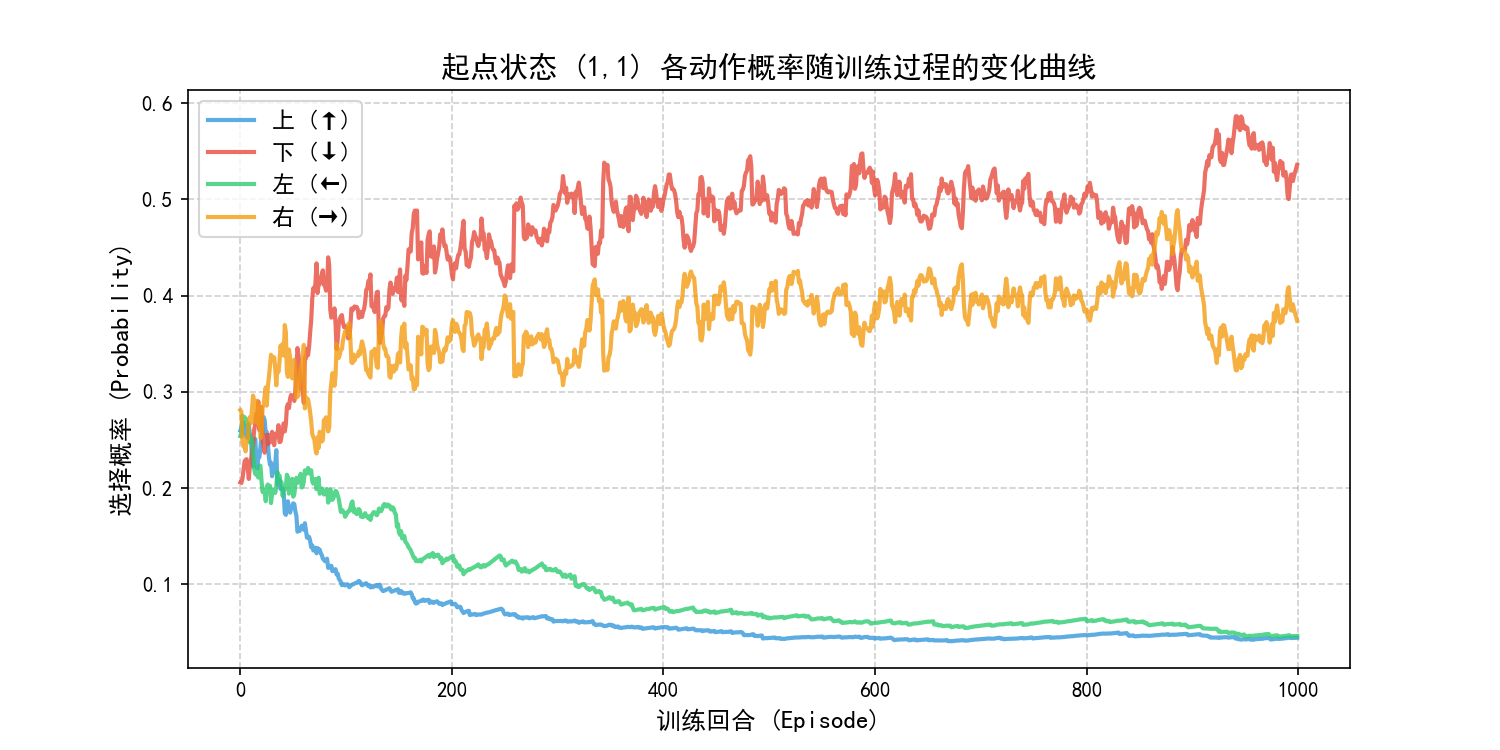
\includegraphics[width=0.75\textwidth]{exp6/results/task3_start_state_probs.png}
\caption{起点状态 (1,1) 各动作概率随训练过程的变化曲线}
\end{figure}

\paragraph{结果分析}
初始阶段四个动作概率均接近 $0.25$。训练至第 1000 回合更新前，起点向下和向右的概率分别约为 $0.536$ 和 $0.374$，向上和向左的概率降至约 $0.044$ 和 $0.046$。策略减少了撞墙动作的概率，但 Softmax 仍为其保留非零概率。

\paragraph{思考题}


\question{问题 1：$\beta_t = \frac{q_t(s_t,a_t)}{\pi(a_t|s_t,\theta_t)}$ 如何同时体现探索和利用？}

\answerlabel 将策略参数的更新量写为
$$\Delta \theta \propto \beta_t \nabla_\theta \pi(a_t|s_t, \theta_t)$$
时，$\beta_t$ 与 $\nabla_\theta\pi$ 的乘积等价于
\[
q_t\nabla_\theta\ln\pi(a_t|s_t,\theta_t).
\]
其中 $q_t$ 根据长期回报强化或抑制本次动作，体现利用；探索来自 Softmax 策略本身对所有动作保留非零采样概率。分母中的 $1/\pi$ 是把概率梯度改写为对数概率梯度的数学因子，并不是额外的探索奖励。低概率动作一旦被采样，其条件更新系数可能较大，但它被采样的频率也更低。

\question{问题 2：当某个动作的累积回报为正时，更新如何影响该动作的概率？当回报为负时呢？}

\answerlabel 以选中动作 $a_t$ 的对数梯度为例：
$$\nabla_{\theta_a} \ln \pi(a_t|s_t, \theta) = \phi(s_t) (\mathbb{I}(a = a_t) - \pi(a|s_t, \theta))$$
当 $q_t>0$ 时，更新提高选中动作的偏好，并相对降低其他动作概率；当 $q_t<0$ 时，更新方向反转，选中动作概率降低，其他动作概率因 Softmax 归一化而相对提高。

\question{问题 3：为什么在回报为负时，低概率动作反而更容易被选中（概率相对增加）？这对探索有何帮助？}

\answerlabel 负回报会降低本次选中动作的偏好。Softmax 对所有动作概率统一归一化，因此该动作概率下降后，其他动作即使参数没有获得同等幅度的直接提升，其归一化概率也会相对增加。

这一再分配使策略在主要动作持续产生负回报时增加尝试其他动作的机会，有助于重新探索。但增加的是相对概率，实际探索程度仍取决于偏好差距、学习率和训练次数。

\question{问题 4：为什么即使最优动作概率很高，策略仍然保持一定的随机性？}

\answerlabel 对有限偏好值，Softmax 输出的每个动作概率都严格大于零。要使某动作概率精确达到 1，需要它与其他动作的偏好差趋于无穷大：
\[
h(s,a^*,\theta)-h(s,a',\theta)\to\infty.
\]
有限步训练通常只能得到接近 1 的概率，因此策略仍保留少量随机性。这使非贪心动作仍可能被采样，但也意味着执行阶段若需要确定性动作，应另行使用贪心策略。

\subsection{核心代码与分析}

\subsubsection{特征提取与偏好函数计算}
偏好函数 $h(s, a, \theta) = \phi(s)^T \theta_a$ 的实现如下，接收一维状态索引，返回大小为 4 的动作偏好数组。
\begin{lstlisting}[language=python]
def get_features(self, s):
    """
    状态特征提取phi(s) = [1, x, y]^T
    x = row + 1, y = col + 1 (行列坐标均转换为1-indexed)
    """
    row, col = divmod(s, self.size)
    x = row + 1.0
    y = col + 1.0
    return np.array([1.0, x, y])

def get_preferences(self, s):
    """
    计算动作偏好 h(s, a, theta) = phi(s)^T * theta_a
    """
    phi = self.get_features(s)
    # self.theta 为 (4, 3) 偏好权重矩阵，phi 为 (3,) 特征向量
    # 点积结果为 4 维向量，代表 4 个动作的偏好
    return np.dot(self.theta, phi)
\end{lstlisting}

\subsubsection{策略概率与动作选择}
利用 Softmax 转换偏好值为动作选择概率，并进行了减去最大值以保证数值稳定性的操作。
\begin{lstlisting}[language=python]
def get_probs(self, s):
    """
    通过 Softmax 函数将偏好值转化为概率
    """
    h = self.get_preferences(s)
    h_stable = h - np.max(h)  # 减去最大值，防止指数爆炸溢出
    exp_h = np.exp(h_stable)
    probs = exp_h / np.sum(exp_h)
    return probs

def choose_action(self, s):
    """
    依据策略概率采样动作
    """
    probs = self.get_probs(s)
    return self.rng.choice(4, p=probs)
\end{lstlisting}

\subsubsection{REINFORCE 的参数更新实现}
在回合结束后，先逆向计算每个时刻的折扣回报 $G_t$，再按任务书公式使用 $\gamma^tG_t$ 完成原始 REINFORCE 更新：
\begin{lstlisting}[language=python]
def update_step(self, s, a, score):
    """
    对单个时间步进行梯度上升更新
    梯度项为：grad = phi * (I(a' == a) - pi(a'|s))
    """
    phi = self.get_features(s)
    probs = self.get_probs(s)
    for a_prime in range(4):
        indicator = 1.0 if a_prime == a else 0.0
        grad = phi * (indicator - probs[a_prime])
        self.theta[a_prime] += self.lr * score * grad

def update_trajectory(self, trajectory, gamma=0.9):
    """
    利用整条轨迹进行 REINFORCE 更新
    """
    T = len(trajectory)
    returns = np.zeros(T)
    g = 0.0
    # 逆向计算折扣回报，提升计算效率
    for t in reversed(range(T)):
        r = trajectory[t][2]
        g = r + gamma * g
        returns[t] = g

    # REINFORCE：直接使用 gamma^t * G_t
    for t in range(T):
        s_t, a_t, _ = trajectory[t]
        score = (gamma ** t) * returns[t]
        self.update_step(s_t, a_t, score)
\end{lstlisting}
\subsection{总结与体会}


这次实验学习了值函数方法与策略梯度方法的对比：值函数方法（如 Q-learning）的目标是逼近动作值函数，存在逼近精度不高时策略抖动剧烈的问题。而策略函数近似能够直接对动作概率进行光滑调整，并能方便地学习到随机策略。

\newpage
\section{Actor-Critic 算法}

\subsection{实验目的与要求}
\begin{enumerate}
\item 理解Actor-Critic框架的核心思想：掌握策略网络（Actor）与价值网络（Critic）的协同工作机制。
\item 掌握QAC算法：能够使用TD方法估计动作价值并同时更新策略参数。
\item 理解基线（Baseline）的作用：掌握优势函数的概念及其方差缩减效果。
\item 实现A2C算法：能够使用状态价值函数作为基线，完成优势Actor-Critic的实现。
\end{enumerate}
\subsection{实验内容与设计}

\subsubsection{公共环境与对比原则}

实验沿用 $5\times5$ GridWorld 和 Softmax Actor。QAC 的 Critic 估计动作价值，A2C 的 Critic 估计状态价值，异策略实验额外使用固定行为策略生成数据。各方法通过总奖励曲线、最终策略和多次运行方差进行比较。

\subsubsection{任务 1：QAC 实验设计}

Actor 使用 Critic 给出的动作价值更新策略参数，Critic 使用 Sarsa TD 目标在线更新。训练记录每回合奖励、状态值和最终策略，并与 REINFORCE 的整回合更新方式比较。

\subsubsection{任务 2：A2C 与基线实验设计}

将 Critic 改为估计 $v(s)$，使用 TD 误差近似优势函数。除比较 QAC 与 A2C 的学习曲线外，还通过多次独立运行的奖励标准差评价基线对方差和训练稳定性的影响。

\subsubsection{任务 3：异策略 Actor--Critic 设计}

固定 $\epsilon$-greedy 行为策略生成 5000 步数据，使用重要性比率修正 Actor 与 Critic 更新，并对权重进行截断。实验比较行为策略与目标策略，并观察过大重要性权重对数值稳定性的影响。




\subsection{实验过程、结果与分析}

\subsubsection{任务 1：QAC 算法实现与分析}

QAC（Q-value Actor-Critic）将 Actor 和 Critic 的功能分离：Critic 用 TD 方法在线估计动作价值 $Q^\pi(s,a)$，Actor 使用 Critic 提供的 $Q$ 值作为策略梯度的评分信号，在每步转移后立即更新策略参数 $\boldsymbol{\theta}$，无需等待 episode 结束。与 REINFORCE 相比，用 TD Critic 替代 MC 回报，大幅降低梯度估计的方差。

在任务 1 中，我们实现了基于 Sarsa 时序差分的 Q Actor-Critic (QAC)。Critic 对每个动作 $a$ 维护一个线性参数 $w_a \in \mathbb{R}^3$，从而动作价值估计为：
$$q(s, a, w) = \phi(s)^T w_a$$
通过采样转移 $(s_t, a_t, r_{t+1}, s_{t+1}, a_{t+1})$ 更新 Critic 权重：
$$\delta_t = r_{t+1} + \gamma \phi(s_{t+1})^T w_{a_{t+1}} - \phi(s_t)^T w_{a_t}$$
$$w_{a_t} \leftarrow w_{a_t} + \alpha_w \delta_t \phi(s_t)$$
Actor 的更新公式为：
$$\theta_c \leftarrow \theta_c + \alpha_\theta \phi(s_t) \left( \mathbb{I}(a_t = c) - \pi(c|s_t, \theta_t) \right) q(s_t, a_t, w_t)$$

\paragraph{学习曲线}
\begin{figure}[H]
\centering
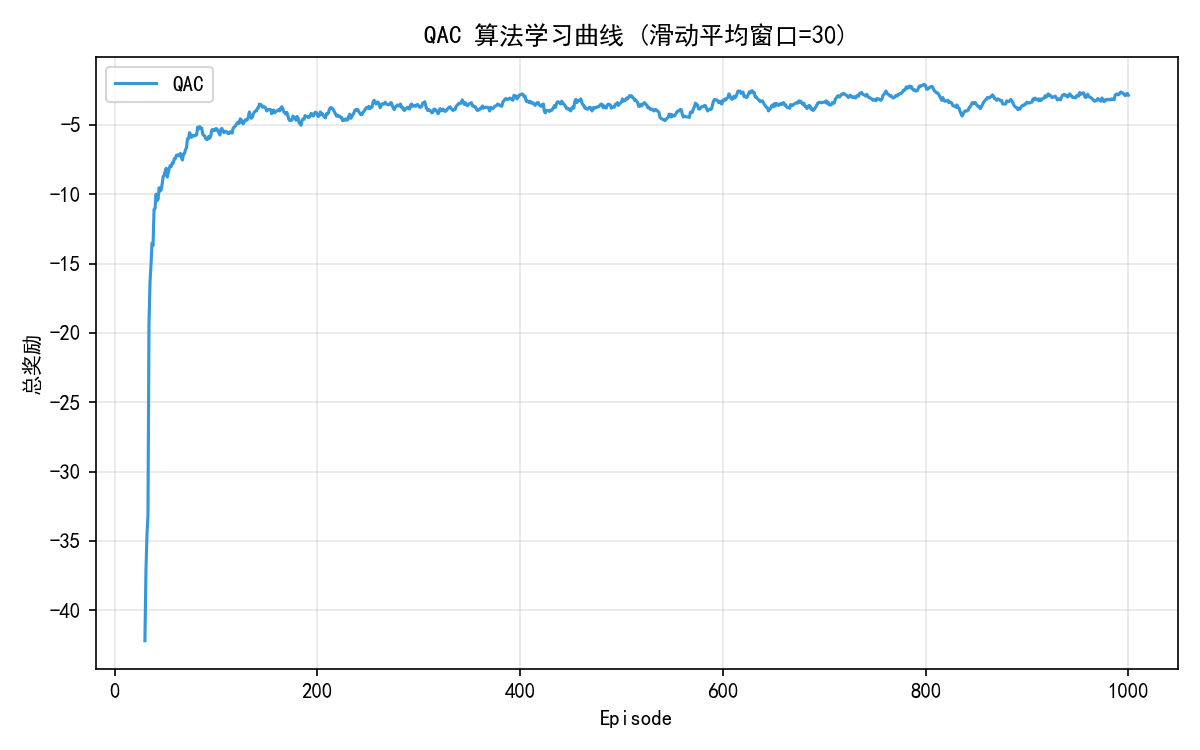
\includegraphics[width=0.65\textwidth]{exp7/results/task1_qac_learning.png}
\caption{QAC学习曲线}
\end{figure}
\paragraph{状态值热力图}
利用 $V(s)=\sum_a\pi(a|s)q(s,a,w)$ 计算最终状态值。
\begin{figure}[H]
\centering
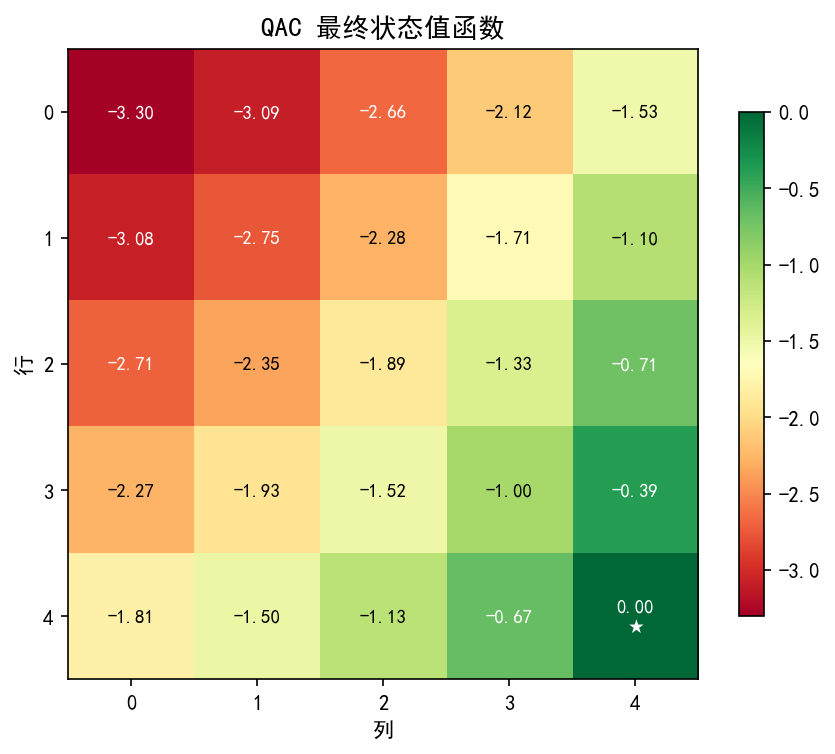
\includegraphics[width=0.4\textwidth]{exp7/results/task1_qac_values.png}
\caption{QAC最终状态值}
\end{figure}
\paragraph{最终贪心策略}
\begin{figure}[H]
\centering
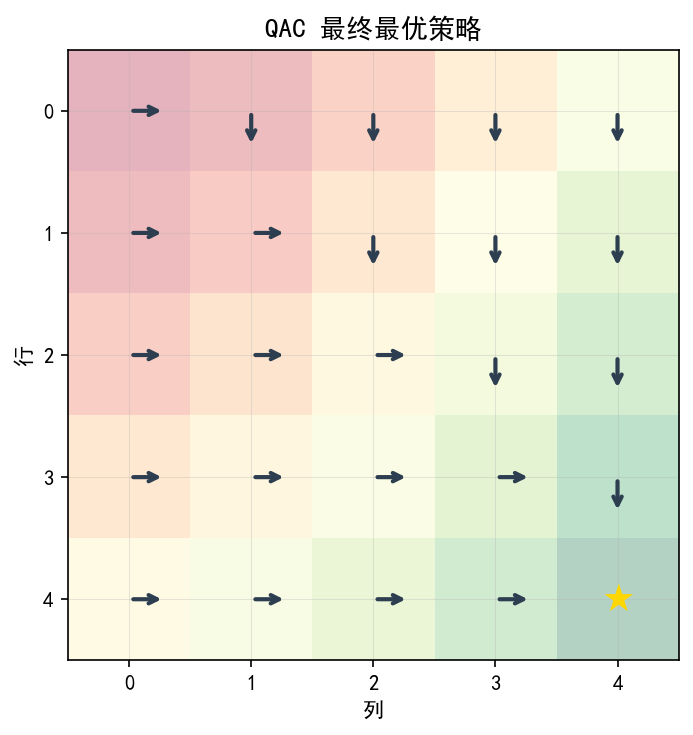
\includegraphics[width=0.4\textwidth]{exp7/results/task1_qac_policy.png}
\caption{QAC最优策略}
\end{figure}

\paragraph{思考题}



\question{问题 1：QAC 与 REINFORCE 在更新方式上有何本质区别？}

\answerlabel REINFORCE 使用完整回合的 Monte Carlo 回报更新策略：
\[
\theta\leftarrow\theta+\alpha G_t\nabla_\theta\ln\pi(a_t|s_t,\theta).
\]
它需要等待 episode 结束，回报包含整条后续轨迹的随机性。

QAC 使用 Critic 估计的动作价值作为评分信号：
\[
\theta\leftarrow\theta+\alpha_\theta q(s_t,a_t,w_t)
\nabla_\theta\ln\pi(a_t|s_t,\theta_t).
\]
Critic 通过 TD 自举逐步更新，因此 QAC 可以在每次转移后更新 Actor。其评分信号通常方差较低，但会受到 Critic 近似误差影响。

\question{问题 2：Critic 的作用是什么？为什么说它“评价”了 Actor 的表现？}

\answerlabel Critic 估计当前策略下的动作价值或状态价值，用于判断某次动作相对于长期目标的效果。在 Actor 更新中，Critic 输出的 $q(s_t,a_t,w_t)$ 或优势估计 $\delta_t$ 作为策略梯度的权重。

评分为正时，Actor 墂大选中动作的概率；评分为负时，Actor 抑制该动作。因此 Critic 并不直接选择动作，而是为 Actor 的策略更新提供评价信号。

\question{问题 3：QAC 中 Actor 和 Critic 分别承担什么角色？它们如何协同工作？}

\answerlabel Actor 表示策略 $\pi(a|s,\theta)$，负责采样动作并更新动作概率；Critic 表示动作价值近似 $q(s,a,w)$，负责根据环境转移更新价值估计。

两者按以下顺序协同更新：
\begin{enumerate}
\item Actor 根据当前策略在状态 $s_t$ 采样并执行动作 $a_t$；
\item Critic 使用转移样本计算 TD 目标并更新价值参数 $w$；
\item Actor 使用 Critic 给出的动作价值作为评分，更新策略参数 $\theta$。
\end{enumerate}
Critic 的估计会随 Actor 改变的策略而变化，Actor 又依赖 Critic 的评价调整策略，因此两组参数需要交替学习。

\subsubsection{任务 2：A2C 算法实现与对比}

A2C（Advantage Actor-Critic）在 QAC 基础上引入优势函数
\[
A^\pi(s,a)=Q^\pi(s,a)-V^\pi(s)
\]
作为策略梯度的评分。减去状态价值基线 $V^\pi(s)$ 可去除与动作无关的背景波动，在保持梯度无偏的同时降低方差。

在任务 2 中，我们引入状态价值基线，将 Critic 改为估计状态价值 $v(s, w) = \phi(s)^T w$，其参数 $w \in \mathbb{R}^3$。
利用 TD 误差近似优势函数：
$$\delta_t = r_{t+1} + \gamma \phi(s_{t+1})^T w_t - \phi(s_t)^T w_t$$
Critic 和 Actor 均由 $\delta_t$ 驱动更新：
$$w \leftarrow w + \alpha_w \delta_t \phi(s_t)$$
$$\theta_c \leftarrow \theta_c + \alpha_\theta \phi(s_t) \left( \mathbb{I}(a_t = c) - \pi(c|s_t, \theta_t) \right) \delta_t$$

我们进行了 10 次独立随机种子实验，比较 QAC 与 A2C 算法在均值和标准差方面的表现。

\begin{table}[H]
\centering
\begin{tabular}{ccC{6.0cm}}
\toprule
算法 & 10次运行平均奖励 & 稳定性与收敛状况分析 \\
\midrule
\textbf{QAC (无基线)} & $-143.1870 \pm 215.2474$ & 平均奖励较低，运行间标准差为 215.25，部分随机种子下曲线出现明显震荡。 \\
\textbf{A2C (含状态价值基线)} & \textbf{$-2.8440 \pm 0.2215$} & 平均奖励较高，运行间标准差为 0.22，在本实验设置下曲线更稳定。 \\
\bottomrule
\end{tabular}
\end{table}

\paragraph{A2C 与 QAC 对比结果}
\begin{figure}[H]
\centering
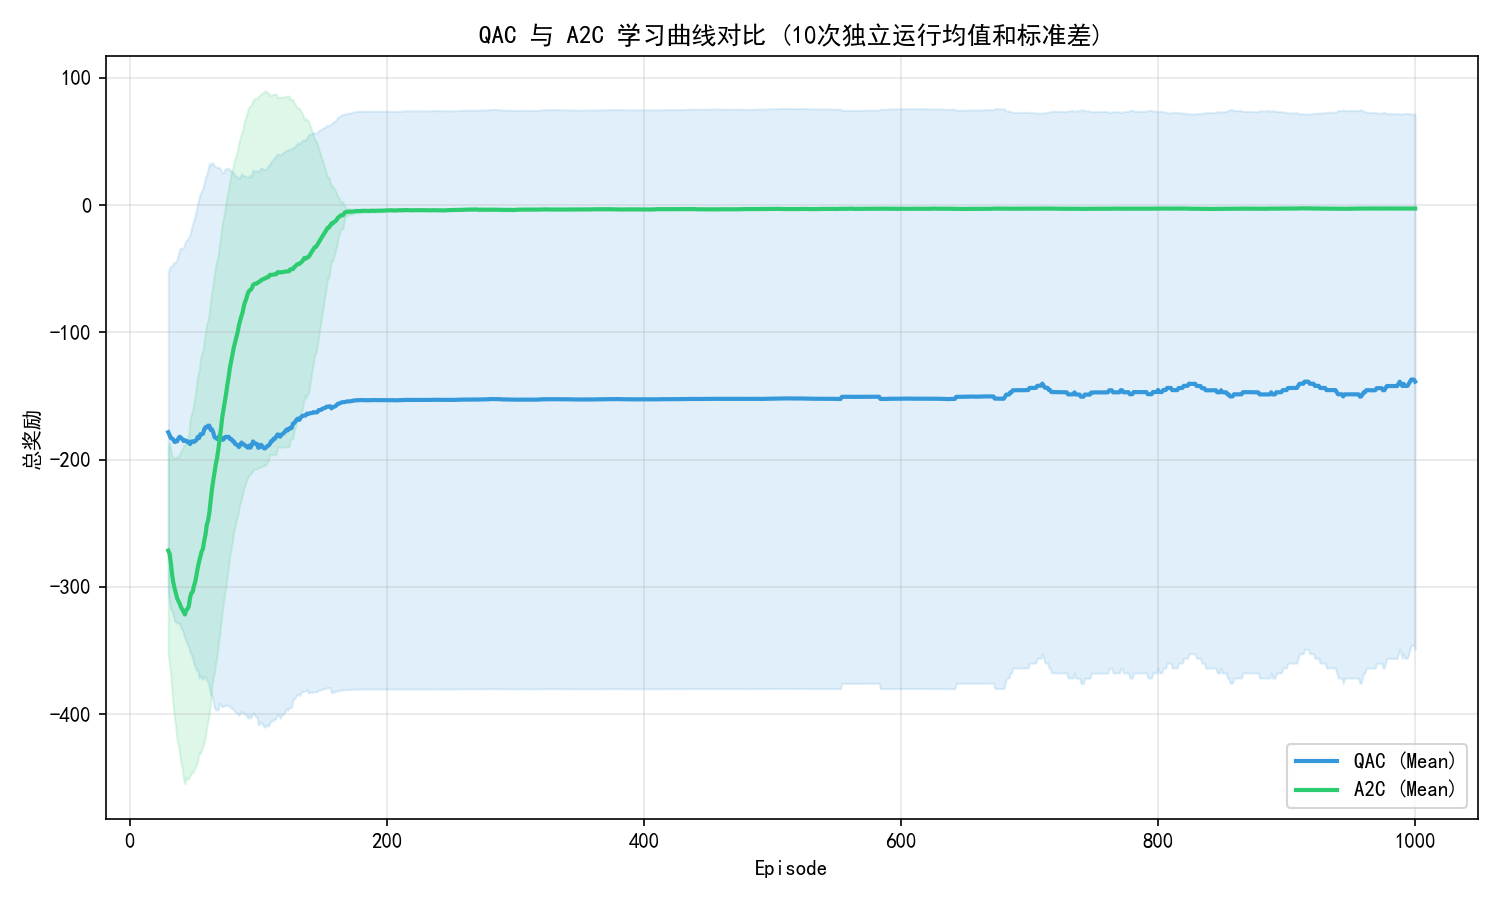
\includegraphics[width=0.8\textwidth]{exp7/results/task2_qac_vs_a2c.png}
\caption{QAC与A2C对比}
\end{figure}
\begin{figure}[H]
\centering
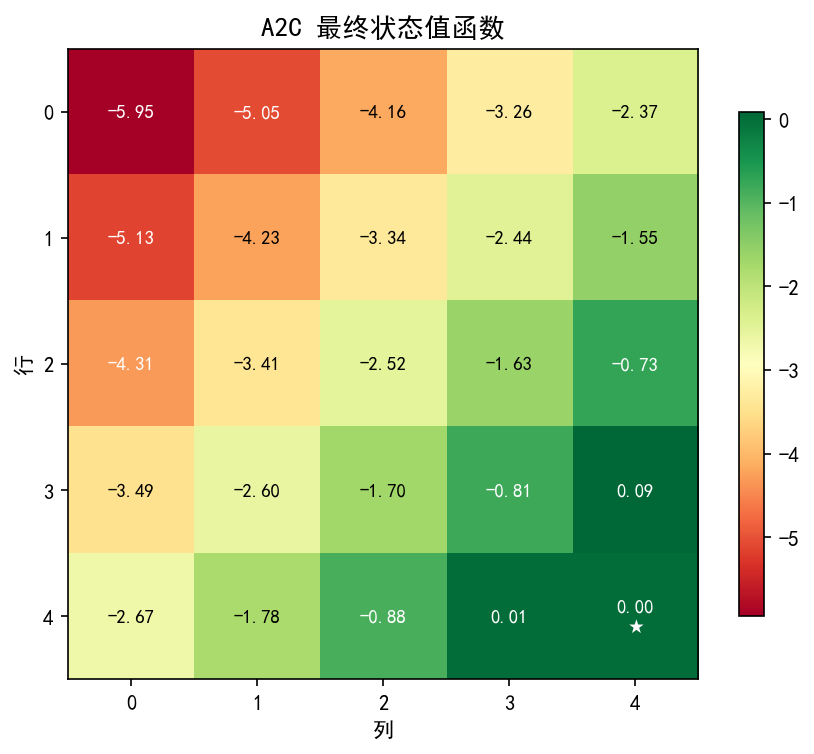
\includegraphics[width=0.5\textwidth]{exp7/results/task2_a2c_values.png}
\caption{A2C最终状态值}
\end{figure}
\begin{figure}[H]
\centering
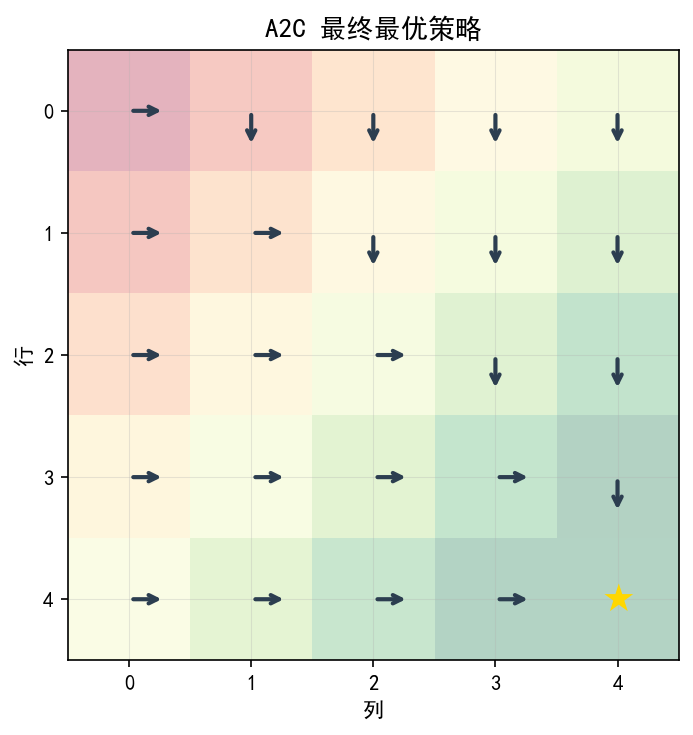
\includegraphics[width=0.4\textwidth]{exp7/results/task2_a2c_policy.png}
\caption{A2C最终最优策略}
\end{figure}

\paragraph{思考题}



\question{问题 1：证明添加基线不改变策略梯度的期望。}

\answerlabel
假设基线函数 $b(S)$ 仅依赖于状态 $S$，与动作 $A$ 无关。我们要证明对任意基线 $b(S)$，其对应的基线梯度的数学期望为 0，即：
$$\mathbb{E}_{A \sim \pi(\cdot|S)} \left[ \nabla_\theta \ln \pi(A|S, \theta) b(S) \right] = 0$$

展开关于动作 $A$ 的条件期望：
$$\mathbb{E}_{A \sim \pi(\cdot|S)} \left[ \nabla_\theta \ln \pi(A|S, \theta) b(S) \right] = \sum_{a \in \mathcal{A}} \pi(a|S, \theta) \nabla_\theta \ln \pi(a|S, \theta) b(S)$$

根据对数梯度的导数关系（Log-Derivative Trick），我们有：
$$\nabla_\theta \ln \pi(a|S, \theta) = \frac{\nabla_\theta \pi(a|S, \theta)}{\pi(a|S, \theta)}$$

将其代入期望展开式中：
$$\sum_{a \in \mathcal{A}} \pi(a|S, \theta) \frac{\nabla_\theta \pi(a|S, \theta)}{\pi(a|S, \theta)} b(S) = \sum_{a \in \mathcal{A}} \nabla_\theta \pi(a|S, \theta) b(S)$$

由于基线 $b(S)$ 仅是状态 $S$ 的函数，与要求和的动作变量 $a$ 无关，因此可以将其提取到求和符号外面：
$$= b(S) \sum_{a \in \mathcal{A}} \nabla_\theta \pi(a|S, \theta) = b(S) \nabla_\theta \sum_{a \in \mathcal{A}} \pi(a|S, \theta)$$

又因为策略是一个概率分布，在状态 $S$ 下所有可能动作的概率之和恒为 1：
$$\sum_{a \in \mathcal{A}} \pi(a|S, \theta) = 1$$

对常数 1 求关于 $\theta$ 的梯度显然为零向量：
$$\nabla_\theta (1) = 0$$

因此：
$$b(S) \nabla_\theta (1) = b(S) \cdot 0 = 0$$

由此得证，在策略梯度中引入任何仅依赖于状态的基线函数 $b(S)$，其梯度期望值均为 0，不会改变策略梯度定理的期望值方向：
$$\mathbb{E}_{A \sim \pi} \left[ \nabla_\theta \ln \pi(A|S, \theta) (q_\pi(S, A) - b(S)) \right] = \mathbb{E}_{A \sim \pi} \left[ \nabla_\theta \ln \pi(A|S, \theta) q_\pi(S, A) \right]$$

\question{问题 2：为什么使用优势函数可以减小方差？基线 $b(s)=v_\pi(s)$ 是最优选择吗？}

\answerlabel 优势函数
\[
A_\pi(s,a)=q_\pi(s,a)-v_\pi(s)
\]
从动作价值中减去该状态下与动作无关的平均水平。这样，优于当前策略平均表现的动作得到正评分，低于平均表现的动作得到负评分，减少了状态本身回报尺度对更新量的影响。

$v_\pi(s)$ 是自然且容易估计的基线，但严格意义下不一定是使方差最小的基线。对给定状态，理论上的最小方差基线为
\[
b^*(s)=
\frac{\mathbb{E}_{A\sim\pi}
\left[\|\nabla_\theta\ln\pi(A|s,\theta)\|^2q_\pi(s,A)\right]}
{\mathbb{E}_{A\sim\pi}
\left[\|\nabla_\theta\ln\pi(A|s,\theta)\|^2\right]}.
\]
由于该量需要额外估计梯度范数加权期望，实际实现通常使用 $v_\pi(s)$ 作为计算代价较低的基线。

\question{问题 3：为什么使用 TD 误差近似优势函数是合理的？}

\answerlabel 根据动作价值的定义和 Bellman 期望方程，有
$$q_\pi(s, a) = \mathbb{E}[R + \gamma v_\pi(S') | s, a]$$
将该式代入优势函数 $A_\pi(s,a)$ 中：
$$A_\pi(s, a) = q_\pi(s, a) - v_\pi(s) = \mathbb{E}[R + \gamma v_\pi(S') | s, a] - v_\pi(s) = \mathbb{E}[R + \gamma v_\pi(S') - v_\pi(s) | s, a]$$
括号内对应 TD 误差
\[
\delta=R+\gamma v_\pi(S')-v_\pi(s).
\]
对单步转移 $(s_t,a_t,r_{t+1},s_{t+1})$，$\delta_t$ 是上述条件期望中的单样本估计。因此，在 Critic 的价值估计足够准确时，可使用 TD 误差近似优势函数；若价值估计存在偏差，该优势估计也会继承相应偏差。

\question{问题 4：A2C 相比 QAC 在训练稳定性上有何改进？}

\answerlabel A2C 使用 TD 误差作为优势估计，使 Actor 根据动作相对于当前状态平均水平的表现进行更新，而不是直接使用动作价值的绝对尺度。该中心化评分可以减少策略梯度的方差。

本实验的 10 次运行结果中，QAC 平均奖励为 $-143.1870\pm215.2474$，A2C 为 $-2.8440\pm0.2215$，说明当前设置下 A2C 的运行间波动明显更小。除基线外，两种 Critic 的参数化形式也不同，因此该差异不能完全归因于单一因素。

\subsubsection{任务 3：异策略 Actor-Critic}

异策略 Actor-Critic 通过\textbf{重要性采样}（Importance Sampling）修正行为策略与目标策略之间的分布偏差：$\rho_t = \frac{\pi(A_t|S_t,\boldsymbol{\theta})}{\mu(A_t|S_t)}$，使得从其他策略（如旧版策略、随机探索策略）收集的历史经验可直接用于更新当前策略，实现数据复用和解耦探索。

行为策略 $\beta(a|s)$ 是对精确 $Q^*(s,a)$ 表（由值迭代求解）施加 $\epsilon=0.3$ 的 $\epsilon$-greedy 策略。我们使用行为策略与环境交互生成 5000 步的固定数据集，包含转移和行为概率。
离线训练时，每次从数据集中抽取转移进行更新，使用重要性采样权重 $\rho_t = \frac{\pi(a_t|s_t, \theta_t)}{\beta(a_t|s_t)}$ 修正 Actor 和 Critic 的更新：
$$w \leftarrow w + \alpha_w \rho_t \delta_t \phi(s_t)$$
$$\theta_c \leftarrow \theta_c + \alpha_\theta \rho_t \phi(s_t) \left( \mathbb{I}(a_t = c) - \pi(c|s_t, \theta_t) \right) \delta_t$$
为了保持数值稳定性，我们在代码中对重要性权重进行了截断限制：$\rho_t \leftarrow \min(\rho_t, 10.0)$。

\paragraph{异策略实验结果}
离线训练评估曲线展示训练过程中目标策略的实际平均累积奖励：
\begin{figure}[H]
\centering
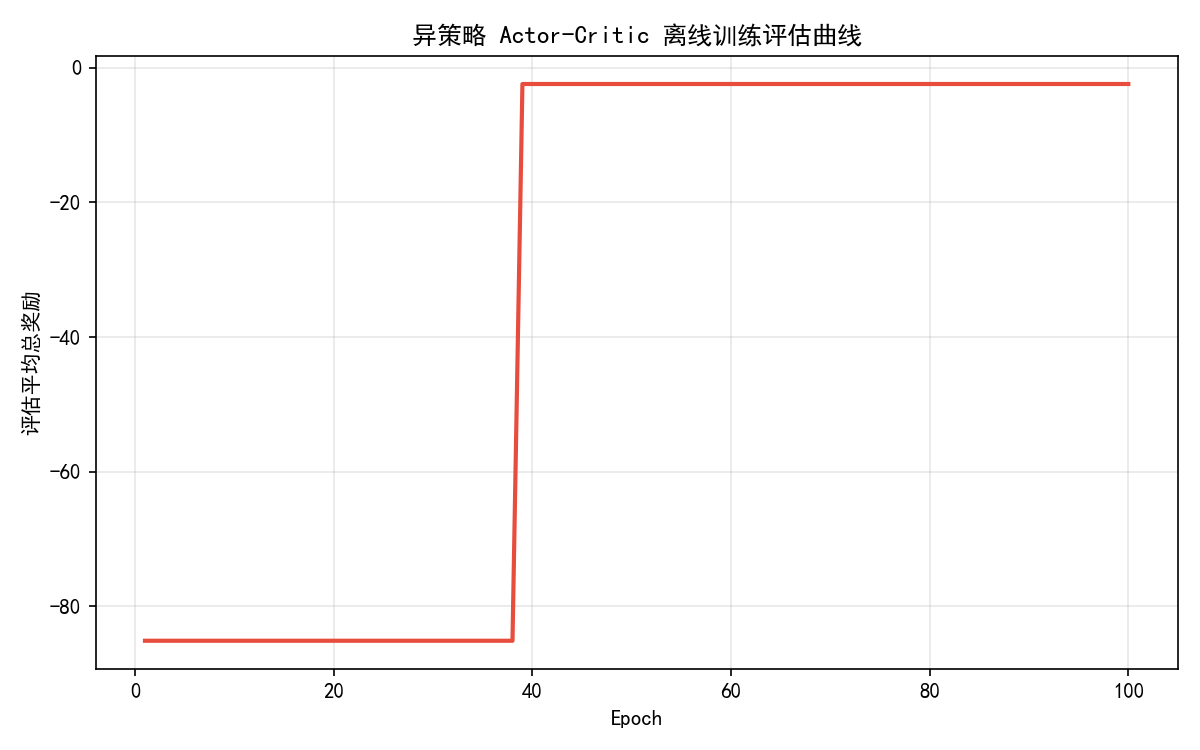
\includegraphics[width=0.75\textwidth]{exp7/results/task3_off_policy_learning.png}
\caption{异策略离线评估}
\end{figure}

\begin{figure}[H]
\centering
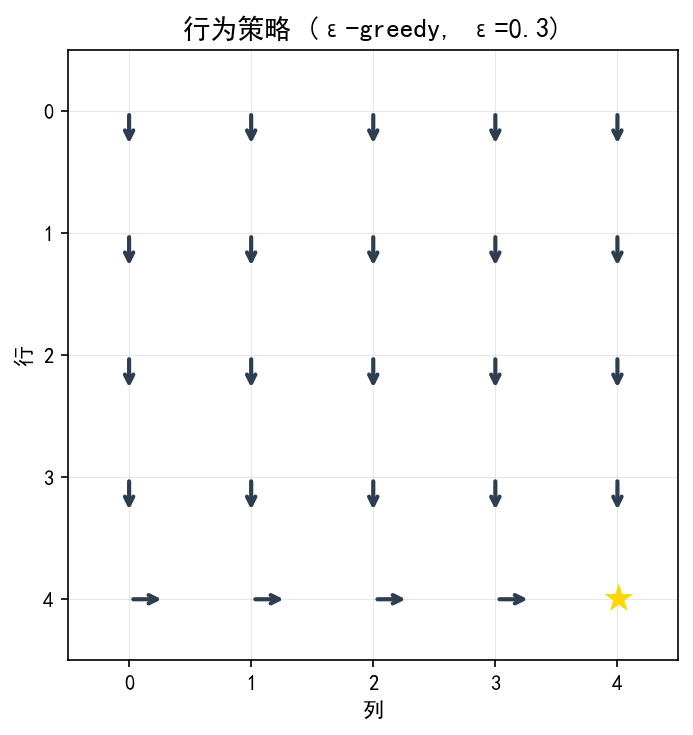
\includegraphics[width=0.4\textwidth]{exp7/results/task3_behavior_policy.png}
\caption{行为策略}
\end{figure}
\begin{figure}[H]
\centering
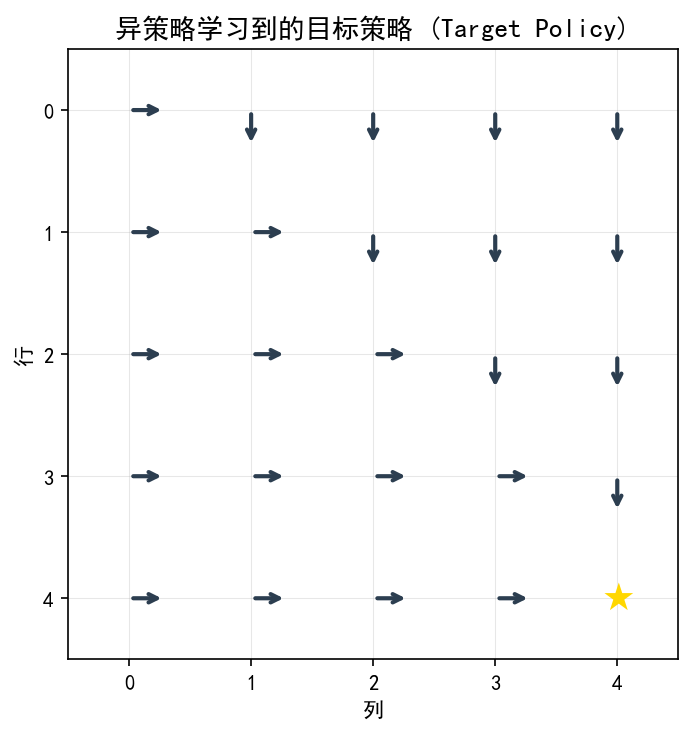
\includegraphics[width=0.4\textwidth]{exp7/results/task3_target_policy.png}
\caption{目标策略}
\end{figure}

\paragraph{思考题}



\question{问题 1：为什么需要重要性采样？异策略 Actor--Critic 相比同策略有什么优势？}

\answerlabel 行为策略 $\beta$ 与目标策略 $\pi$ 的动作概率不同，直接使用 $\beta$ 生成的样本估计 $\pi$ 下的更新会产生分布偏差。重要性比率
\[
\rho_t=\frac{\pi(a_t|s_t)}{\beta(a_t|s_t)}
\]
根据两种策略对已采样动作的相对概率调整样本贡献，使行为策略数据可用于近似目标策略下的期望。

异策略方法的主要优势是可以分离数据收集与策略优化，并重复使用由其他策略生成的数据。本实验使用固定行为策略收集的 5000 步数据更新目标策略，体现了这一点。该能力依赖行为数据覆盖目标策略需要的状态--动作区域；覆盖不足时，重要性采样无法补充未出现的数据。

\question{问题 2：重要性权重的作用是什么？什么情况下重要性权重会很大？}

\answerlabel 重要性权重用于调整行为策略样本在目标策略更新中的贡献。当目标策略对已采样动作赋予的概率高于行为策略时，$\rho_t>1$，该样本的更新被放大；反之则被减小。

当 $\pi(a|s)$ 较大而 $\beta(a|s)$ 很小时，比率会很大。例如 $\pi(a|s)=0.95$、$\beta(a|s)=0.05$ 时，$\rho=19$。大权重会放大单样本噪声并提高更新方差，因此本实验将其截断为 10。截断有助于数值稳定，但也会引入偏差。

\question{问题 3：异策略 Actor--Critic 为什么能利用历史数据？}

\answerlabel 历史数据通常由旧策略或其他行为策略生成，其分布与当前目标策略不同。若记录了行为策略对已执行动作的概率，就可以计算重要性比率，并对这些样本在当前目标策略更新中的贡献进行修正。

因此，异策略 Actor--Critic 可以重复使用固定数据集或经验回放中的旧样本。不过，这并不意味着任意历史数据都有效：行为概率必须可知，且数据需要覆盖目标策略关注的状态--动作对。

\subsection{核心代码与分析}

\subsubsection{QAC 动作选择与 Actor 更新}
在 QAC 算法中，Actor 使用 Softmax 计算概率，并按照如下代码进行对数梯度的策略更新（引入了折扣追踪器 \texttt{I}）：
\begin{lstlisting}[language=python]
def softmax_policy(s, theta, env):
    phi = get_state_feature(s, env)  # 获取状态特征 [1, x, y]
    h = theta.dot(phi)              # 计算动作偏好
    h_stable = h - np.max(h)        # 减去最大值，避免数值溢出
    exp_h = np.exp(h_stable)
    probs = exp_h / np.sum(exp_h)   # Softmax 归一化
    return probs

# Actor 更新代码段
for c in range(num_actions):
    # 对数策略梯度公式：grad = phi * (I(a == c) - pi(c|s))
    grad_ln_pi = phi_s * ((1.0 if c == a else 0.0) - probs[c])
    # 策略梯度上升更新（含折扣追踪器 I）：theta = theta + alpha * I * grad * Q(s, a)
    theta[c] += alpha_theta * I * grad_ln_pi * q_sa
\end{lstlisting}
\textbf{数学公式对应关系}：
对数梯度计算对应于：
$$\nabla_{\theta_c} \ln \pi(a|s, \theta) = \phi(s) \left( \mathbb{I}(a = c) - \pi(c|s, \theta) \right)$$
更新策略权重对应于（含折扣因子权重）：
$$\theta_{t+1} = \theta_t + \alpha_\theta \gamma^t \nabla_\theta \ln \pi(a_t | s_t, \theta_t) q(s_t, a_t, w_t)$$
\subsubsection{A2C 优势函数计算与 Critic 更新}
在 A2C 中，Critic 仅估计状态价值，使用单步 TD 误差作为优势函数估计，并使用折扣追踪器 \texttt{I} 进行 Actor 更新：
\begin{lstlisting}[language=python]
# A2C 核心单步更新逻辑
phi_s = get_state_feature(s, env)
v_s = phi_s.dot(w)  # Critic 计算当前状态价值 V(s)

s_next, r = env.step(s, a)

if env.is_terminal(s_next):
    delta = r - v_s  # 终止状态下下一状态价值为 0，优势值 delta = r - V(s)
    w += alpha_w * delta * phi_s  # Critic 参数更新
    # Actor 更新
    for c in range(num_actions):
        grad_ln_pi = phi_s * ((1.0 if c == a else 0.0) - probs[c])
        theta[c] += alpha_theta * I * grad_ln_pi * delta
else:
    phi_s_next = get_state_feature(s_next, env)
    v_s_next = phi_s_next.dot(w)  # 计算 V(s')
    
    delta = r + env.gamma * v_s_next - v_s  # TD误差近似优势值 delta = r + gamma * V(s') - V(s)
    
    w += alpha_w * delta * phi_s  # Critic 状态价值更新
    # Actor 策略更新
    for c in range(num_actions):
        grad_ln_pi = phi_s * ((1.0 if c == a else 0.0) - probs[c])
        theta[c] += alpha_theta * I * grad_ln_pi * delta
    
    s = s_next
    I *= env.gamma  # 更新折扣因子追踪器
\end{lstlisting}
\textbf{数学公式对应关系}：
TD 误差（即优势估计）对应：
$$\delta_t = r_{t+1} + \gamma v(s_{t+1}, w) - v(s_t, w)$$
价值权重更新对应：
$$w \leftarrow w + \alpha_w \delta_t \phi(s_t)$$
策略权重更新对应：
$$\theta_{t+1} = \theta_t + \alpha_\theta \gamma^t \nabla_\theta \ln \pi(a_t | s_t, \theta_t) \delta_t$$
\subsubsection{异策略 Actor-Critic 重要性比率修正}
在 \texttt{task3\_off\_policy.py} 中，使用重要性采样权重 $\rho_t$ 对 Actor 和 Critic 更新进行了修正：
\begin{lstlisting}[language=python]
# 计算目标策略选择当前动作 a 的概率
pi_probs = softmax_policy(s, theta, env)
pi_a = pi_probs[a]

# 计算重要性权重比率 rho = pi(a|s) / beta(a|s)
rho = pi_a / beta_a
rho = np.clip(rho, 0.0, 10.0)  # 进行重要性权重截断，防止大梯度导致训练发散

# 使用重要性采样比率修正更新
w += alpha_w * rho * delta * phi_s  # Critic 更新引入重要性权重 rho

for c in range(num_actions):
    grad_ln_pi = phi_s * ((1.0 if c == a else 0.0) - pi_probs[c])
    theta[c] += alpha_theta * rho * grad_ln_pi * delta  # Actor 更新引入重要性权重 rho
\end{lstlisting}
\textbf{数学公式对应关系}：
重要性权重对应于：
$$\rho_t = \frac{\pi(a_t | s_t, \theta_t)}{\beta(a_t | s_t)}$$
Actor 异策略更新对应于：
$$\theta_{t+1} = \theta_t + \alpha_\theta \rho_t \nabla_\theta \ln \pi(a_t | s_t, \theta_t) \delta_t$$
\subsection{总结与体会}

\begin{enumerate}
\item \textbf{折扣追踪器 $I = \gamma^t$ 的影响}：
   在最初的实验中，我们发现不带折扣追踪器 $I$ 的 QAC 和 A2C 算法极易陷入早期策略崩溃，策略退化为只选择 “向上” 或 “向左” 的次优甚至死循环策略。经深入分析，其根本原因在于 $\phi(s) = [1, x, y]^T$ 作为线性特征时，特征值在接近终点（右下角）时增大到 5 倍，且早期随机探索阶段的大量负奖励使得 Critic 输出的 $Q$ 值或 $V$ 值均为负。如果没有 $\gamma^t$ 对轨迹后期的 Actor 梯度更新进行指数衰减，由于终点附近动作特征幅度巨大，其产生的负梯度更新极易压倒一切，使 Actor 彻底丧失向右和向下的偏好。
   引入折扣追踪器 $I=\gamma^t$ 后，轨迹后段的 Actor 更新权重随时间衰减，减弱了终点附近较大坐标特征和负回报对参数的影响。在本实验中，加入该因子后 QAC 与 A2C 的奖励曲线更稳定，并得到可到达目标的策略；这一现象说明实现细节需要与所采用的折扣目标保持一致。
\item \textbf{策略梯度与自举的平衡}：在实验中我们体会到，经典的 Actor-Critic 结合了策略梯度（无偏但高方差）和时序差分自举（有偏但低方差）的优点，通过将累积期望回报 $G_t$ 替换为 Critic 学习到的价值函数，能够在大维度或连续动作状态空间下提供高效的学习模式。
\item \textbf{基线对稳定性的影响}：10 次独立运行中，QAC 的平均奖励为 $-143.1870\pm215.2474$，A2C 为 $-2.8440\pm0.2215$。在本实验设置下，状态价值基线显著降低了运行间方差，并使奖励曲线更稳定。
\item \textbf{异策略扩展的结果}：异策略 Actor-Critic 能够从固定 $\epsilon$-greedy 行为策略的数据中改进目标策略；重要性采样截断限制了单步更新幅度。该结果依赖行为数据对相关状态--动作对的覆盖程度。
\end{enumerate}

\end{document}
